In this chapter we introduce a technique for improving the scalability of safety validation algorithms for multi-agent systems. We first describe the problem of exponential growth of states and disturbances with respect to the number of adversarial entities. We then show how multi-agent safety validation problems can be decomposed into subproblems each involving the system interacting with a subset of the adversaries. The solution to these subproblems can be recombined using an attention network and a base network to correct for multi-agent interactions. We demonstrate the efficacy of scene decomposition by approximating the distribution over failures of a multi-agent gridworld and T-intersection scenario. 

\section{Motivation}

%todo:cite airspace density commment below
Many of the most exciting use cases for autonomy require the system to interact with large number of other human and non-human agents. An autonomous driving policy must reason about a potentially large number other vehicles, pedestrians, cyclists, and traffic control systems, each with a wide variety of possible behaviors. Similarly, autonomous aircraft will soon have to navigate and avoid collisions in an increasingly dense airspace.

Many of the challenges for safety validation are exacerbated when the environment contains multiple interacting agents. The dimensionality of both the disturbance and state space grows with each new agent in the environment. The search over disturbance trajectories, state-dependent policies, or the state space itself can quickly become intractable. Failures may be more or less likely with more agents, but the fraction of the disturbance trajectory space that leads to a failure will likely decrease due to the dramatic increase in the size of the disturbance trajectory space. 

As an example, consider the $5 \times 5$ adversarial gridworld problem depicted in \cref{fig:ch6_fullg} where an ego agent (blue) tries to avoid two adversarial agents (orange and red).  Each agent has a 2D position and four possible actions so the state space and disturbance space both grow exponentially with the number of agents. In this case, a failure occurs when all agents overlap on the same state, so failures become less likely with the number agents. Value iteration is tractable on this problem with two adversaries (which is why we include it as a test case), but becomes challenging with \num{3} agents and intractable with more.

The curse of dimensionality is a well known problem in multi-agent systems and is often solved by decomposing the problem into simpler problems that are tractable and then recombining the solutions. In this chapter we develop a technique for decomposing and recombining safety validation problems. The basic idea is to identify a natural decomposition of the state space that reduces the full problem into a set of subproblems that can be solved individually. For example, the gridworld with two adversaries can be decomposed into two gridworlds, each with a single adversary (as shown in \cref{fig:ch6_subg1,fig:ch6_subg2}). Then, to solve the full problem we learn how to combine the subproblem solutions instead of solving the problem from scratch. The solution to the full problem may not be a simple combination of the subproblem solutions so we simultaneously learn a correction factor. 

For this procedure to be successful, however, we need the subproblem solutions to confer some benefit to the solution of the full problem. In the case of the gridworld example, the subproblem solutions will suggest that it is beneficial to move toward the ego to cause failure. This insight will likely aid the adversary when solving the full problem.

In the next section we formalize the decomposition and highlight some potential efficiencies. We then demonstrate that combining the subproblems can be cast as a transfer learning problem and we apply a known transfer learning algorithm to solve it. 


\begin{figure*}
    \centering
    \begin{subfigure}[b]{0.25\textwidth}
        \centering
        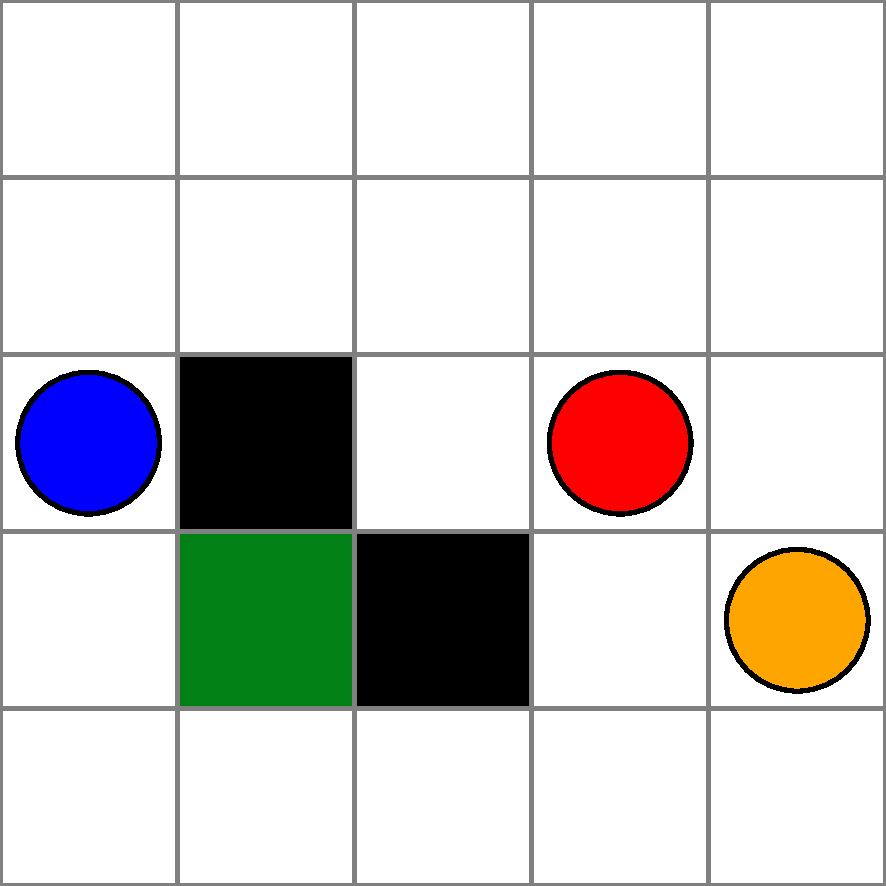
\includegraphics[width=\textwidth]{figures/problem_decomposition/g.pdf}
        \caption{Full problem.}
        \label{fig:ch6_fullg}
    \end{subfigure}
    \hfill
    \begin{subfigure}[b]{0.25\textwidth}
        \centering
        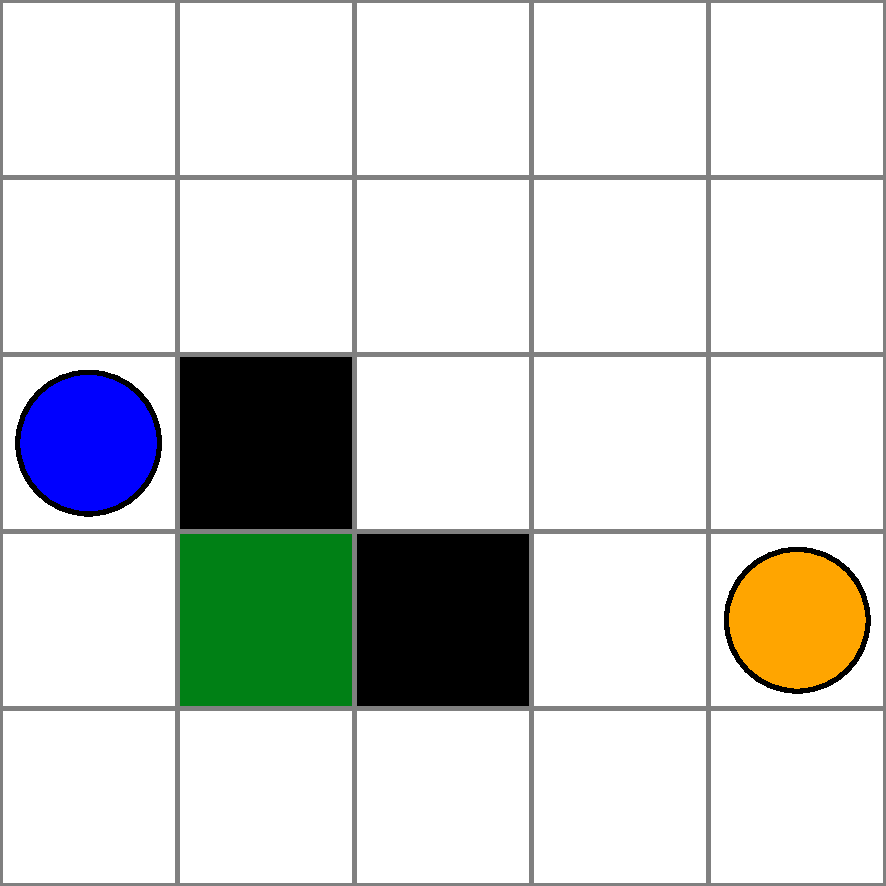
\includegraphics[width=\textwidth]{figures/problem_decomposition/g_sub1.pdf}
        \caption{Subproblem 1}
        \label{fig:ch6_subg1}
    \end{subfigure}
    \hfill
    \begin{subfigure}[b]{0.25\textwidth}
        \centering
        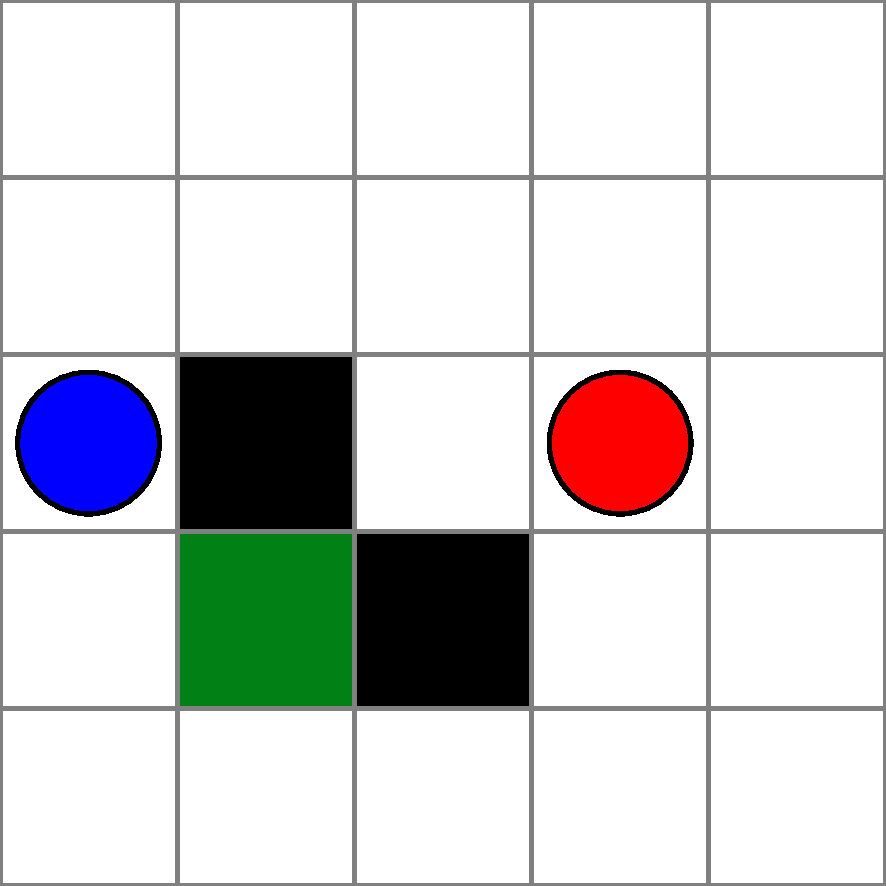
\includegraphics[width=\textwidth]{figures/problem_decomposition/g_sub2.pdf}
        \caption{Subproblem 2.}
        \label{fig:ch6_subg2}
    \end{subfigure}
    \caption{Example decomposition of the gridworld with two adversaries.}
    \label{fig:adv_gridworld_decomp}
\end{figure*}

\section{Decomposition and Fusion}
In this section we describe the process of problem decomposition and identify situations where subproblems are identical. We then introduce the attend, adapt, and transfer algorithm that automatically learns how to combine the subproblem solutions while learning a correction factor. 

\subsection{Problem Decomposition}
The goal of state-space decomposition is to identify a set of subspaces that each represent a similar, but smaller, version of the full problem. We denote the state space of the $i$th subproblem $S^{(i)}$ and the disturbance space $X^{(i)}$. The state $s^{(i)} \in S^{(i)}$ contains the components of $s$ that are associate with the $i$th subproblem and similarly for the disturbance $x^{(i)}$. A crucial constraint on the choice of decomposition is the ability to simulate transitions of the subproblems
\begin{equation}
    s_{t+1}^{(i)} \sim P( s^{(i)} \mid s_t^{(i)}, x_t^{(i)} ) \text{.}
\end{equation}

In the gridworld example, if we choose a decomposition where the state space consists only of the horizontal component of each agent, it is not clear how we would choose a transition model that is faithful to the original problem. Instead, if we choose a decomposition where the state space is the position of the ego and one adversary, and the disturbance space is the disturbance space of that adversary then we have reduced the problem a single-adversary gridworld which we know how to simulate. Indeed, in multi-agent problems a natural decomposition usually consists of the state spaces from a subset of of the agents. 

In some cases, multiple subproblems will reduce to the same problem and only one solution will be required. For example, suppose we wish to solve for the probability of failure at each state in a gridworld with $N$ adversarial agents. If we decompose it into $N$ gridworlds (each with the ego and one adversary), then each subproblem is identical (assuming the ego agent cannot distinguish adversaries). Noticing these overlaps can save a significant amount of computational effort when computing subproblem solutions. The next section describes how to combine subproblem solutions once they are computed. 

\subsection{Solution Fusion}
We now assume that we have decomposed the safety validation problem into $M$ subproblems and obtained a solution $K$ for each. We assume that solution takes the form of a policy or a value function that solves the associated subproblem. For falsification and most-likely failure analysis tasks, $K$ should produce the lowest cost failure trajectories. When approximating the distribution over failures $K$ may estimate the probability of failure at each state or be the distribution over failures of the subproblem. Then, the goal is to use the $M$ subproblems to learn the solution to the full problem 
\begin{equation}
K_{\rm full} = \mathcal{L}(K_1, \ldots, K_M) \label{eq:ch6_solution_fusion}
\end{equation}
with some learning algorithm $\mathcal{L}$. Fortunately, this problem formulation is the same as transfer learning, which has many existing solution techniques~\cite{taylor2009transfer}.

% Intro to A2T
In safety validation, the full problem may contain failure modes that arise from the complex interaction of multiple agents and are therefore not present in the subproblems. The solutions to the subproblems may not contain the needed information for finding failures in the full problem and may even make it more difficult to find failures (an effect known as negative transfer). From these considerations we selected the attend, adapt, and transfer algorithm (A2T)~\cite{rajendran2017attend}. A2T combines solutions using a learned set of attention weights that can minimize negative transfer, and simultaneously learns a new solution from scratch to account for the complexities of the full problem. 

With A2T, the full solution at state $s$ is given by 
\begin{equation}
K_{\rm full}(s) = w_0(s) K_{\rm base}(s) + \sum_{i=1}^M w_i(s) K_i(s^{(i)}) \label{eq:ch6_a2t}
\end{equation}
where $w(s)$ is a state-dependent attention weight and $K_{\rm base}$ is the solution learned from scratch. \cref{eq:ch6_a2t} can be encoded as the network architecture shown in \cref{fig:ch6_A2T_Network}. The state is passed to the base network, the set of subproblem solutions, and an attention network. The base network outputs $K_{\rm base}(s)$ while the subproblem solutions output $K_i(s^{(i)}$. The attention network outputs the attention weights $w_i(s)$ which are combined with $K_{\rm base}$ and $K_i$ to get the full solution $K_{\rm full}(s)$. The parameters in the base network and the attention network can be optimized through backpropagation (as indicated by the dashed lines), using any typical learning algorithm such as DQN or policy gradient methods.

\begin{figure}[!t]
\centering
% TikZ diagram for black-box safety validation problem formulation.
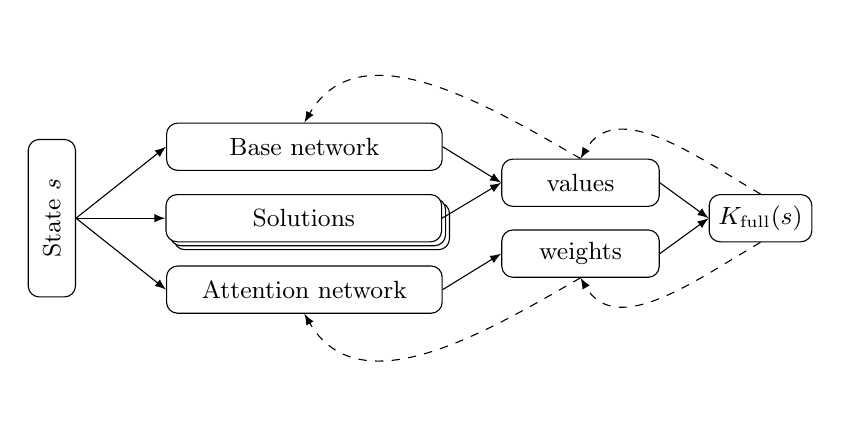
\begin{tikzpicture}
    \tikzstyle{every node}=[font=\small, align=center]
    \tikzset{
        n/.style={draw, rounded corners, minimum height=0.6cm, minimum width = 2cm},
        n2/.style={n, minimum width=3.5cm}
        }
    
    %state 
    \node (state) [n, rotate=90] {\small State $s$};
    
    %base network
    \node (base) [n2, above right of=state, xshift=2.5cm, yshift = 0.2cm] {Base network};
    
    %Solutions
    \node (solutionsback1) [n2, right of=state, xshift=2.3cm, yshift=-0.1cm] {};
    \node (solutionsback2) [n2, fill=white, right of=state, xshift=2.25cm, yshift=-0.05cm] {};
    \node (solutions) [n2, fill=white, right of=state, xshift=2.2cm] {Solutions};
    
    %weights
    \node (attn) [n2, below right of=state, xshift=2.5cm, yshift=-0.2cm] {Attention network};
    

    \node (values) [n, below right of=base, xshift=2.8cm, yshift = 0.25cm] {values};
    
     \node (weights) [n, above right of=attn, xshift=2.8cm, yshift = -0.25cm] {weights};
     
     \node (pfail) [n, minimum width = 0.5cm, right of=state, xshift=8cm] {$K_{\rm full}(s)$};
    

    \draw[-latex] (state.south) -- (base.west);
    \draw[-latex] (state.south) -- (solutions.west);
    \draw[-latex] (state.south) -- (attn.west);
    
    \draw[-latex] (base.east) -- (values.west);
    \draw[-latex] (solutions.east) -- (values.west);
    \draw[-latex] (attn.east) -- (weights.west);
    
    \draw[-latex] (weights.east) -- (pfail.west);
    \draw[-latex] (values.east) -- (pfail.west);
    
    
    % backprop
    
    \draw [dashed, -latex] (weights.south) to [out=-150,in=-60] (attn.south);
    \draw [dashed, -latex] (pfail.south) to [out=-150,in=-60] (weights.south);
    \draw [dashed, -latex] (values.north) to [out=150,in=60] (base.north);
    \draw [dashed, -latex] (pfail.north) to [out=150,in=60] (values.north);
\end{tikzpicture}
\caption{The A2T network. }
\label{fig:ch6_A2T_Network}
\end{figure}


\section{Experiments}

In this section we perform experiments to investigate the benefit of problem decomposition for approximating the distribution over failures. As discussed in \cref{ch5}, to approximate the distribution over failures we need to estimate the probability of failure at each state. The solutions $K_i(s)$ will represent the probability of failure for each disturbance from state $s$. 

In the first experiment we use the gridworld scenario with two adversaries because it can be solved with exact value iteration. Having the ground truth allows us to compare estimates of the probability of failure with and without the subproblem solutions. In the second experiment we solve for the distribution over failures in the T-intersection with \num{4} adversaries and show it outperforms our baseline approaches. Lastly, we demonstrate that the attention network may also lend a degree of interpretability to the safety validation results. 

\subsection{Adversarial Gridworld Example}

The goal of this experiment is to compare the estimates of the probability of failure between a basic neural network and an A2T network that uses estimates of the probability of failure from decomposed subproblems. To make the comparison, we use value iteration to obtain the ground truth $P_{\rm fail}(s)$ of a $5 \times 5$ gridworld with \num{2} adversaries and an expert ego policy. 

As previously described, the gridworld can be decomposed into two identical gridworlds each with a single adversary (\cref{fig:adv_gridworld_decomp}). We solve for the probability of failure for each state and disturbance of the single-adversary problem $P^{\rm sub}_{\rm fail}(s^{(i)}, x^{(i)})$ using exact value iteration. The A2T estimate of the probability of failure is then given by
\begin{equation}
\begin{split}
    P^{\rm A2T}_{\rm fail}(s, x) = w_0(s) P_{\rm fail}^{\rm base}(s, x) &+ \sum_{i=1}^2 w_i(s) P^{\rm sub}_{\rm fail}(s^{(i)}, x^{(i)}) \\
    &+ w_3(s) P^{\rm sub}_{\rm fail}(s^{(1)}, x^{(1)})P^{\rm sub}_{\rm fail}(s^{(2)}, x^{(2)})
\end{split}
\end{equation}
where we included the last term to help model the conjunctive nature of the failure mode of the full problem. 

The attention network has a single hidden layer with \num{32} units and has a softmax layer at the output to normalize the weights. The base network has two hidden layers with \num{64} and \num{32} units and relu activations. The base network has sigmoid activations on the last layer to ensure the output is bounded in $(0,1)$. The A2T network is compared against a neural network with same architecture as the base network. Both networks were trained using our version of DQN for $P_{\rm fail}$ estimation (see \cref{ch5}). We trained for \num{1e5} steps with the ADAM optimizer and a learning rate of \num{1e-3}. 

During training we periodically computed the mean square log error between the estimate and the ground truth and plotted the results in \cref{fig:ch6_adv_gridworld_training}. We first notice that the A2T network reaches its lowest error more quickly than the basic network, but more importantly, remains close to this error for the rest of training, likely because it is near a local minimum. The basic network initially reduces in error but eventually goes unstable and does not converge to a minimum. The use of subproblem solutions speeds up the training process and appears to improve the training stability as well. We now perform some experiments on the T-intersection problem to more fully demonstrate the problem decomposition technique.

\begin{figure}
        \centering
        \begin{tikzpicture}[/tikz/background rectangle/.style={fill={rgb,1:red,1.0;green,1.0;blue,1.0}, draw opacity={1.0}}, show background rectangle]
\begin{axis}[point meta max={nan}, point meta min={nan}, legend cell align={left}, title={MSLE Over Training}, title style={at={{(0.5,1)}}, anchor={south}, font={\large}, color={rgb,1:red,0.0;green,0.0;blue,0.0}, draw opacity={1.0}, rotate={0.0}}, legend style={color={rgb,1:red,0.0;green,0.0;blue,0.0}, draw opacity={1.0}, line width={1}, solid, fill={rgb,1:red,1.0;green,1.0;blue,1.0}, fill opacity={1.0}, text opacity={1.0}, font={\normalsize}, at={(0.98, 0.98)}, anchor={north east}}, axis background/.style={fill={rgb,1:red,1.0;green,1.0;blue,1.0}, opacity={1.0}}, anchor={north west}, xshift={1.0mm}, yshift={-1.0mm}, width={150.4mm}, height={70.6mm}, scaled x ticks={false}, xlabel={Training Steps}, x tick style={color={rgb,1:red,0.0;green,0.0;blue,0.0}, opacity={1.0}}, x tick label style={color={rgb,1:red,0.0;green,0.0;blue,0.0}, opacity={1.0}, rotate={0}}, xlabel style={at={(ticklabel cs:0.5)}, anchor=near ticklabel, font={\normalsize}, color={rgb,1:red,0.0;green,0.0;blue,0.0}, draw opacity={1.0}, rotate={0.0}}, xmajorgrids={true}, xmin={-2468.0299999999997}, xmax={102473.03}, xtick={{0.0,25000.0,50000.0,75000.0,100000.0}}, xticklabels={{$0$,$2.5\times10^{4}$,$5.0\times10^{4}$,$7.5\times10^{4}$,$1.0\times10^{5}$}}, xtick align={inside}, xticklabel style={font={\normalsize}, color={rgb,1:red,0.0;green,0.0;blue,0.0}, draw opacity={1.0}, rotate={0.0}}, x grid style={color={rgb,1:red,0.0;green,0.0;blue,0.0}, draw opacity={0.1}, line width={0.5}, solid}, axis x line*={left}, x axis line style={color={rgb,1:red,0.0;green,0.0;blue,0.0}, draw opacity={1.0}, line width={1}, solid}, scaled y ticks={false}, ylabel={MSLE}, y tick style={color={rgb,1:red,0.0;green,0.0;blue,0.0}, opacity={1.0}}, y tick label style={color={rgb,1:red,0.0;green,0.0;blue,0.0}, opacity={1.0}, rotate={0}}, ylabel style={at={(ticklabel cs:0.5)}, anchor=near ticklabel, font={\normalsize}, color={rgb,1:red,0.0;green,0.0;blue,0.0}, draw opacity={1.0}, rotate={0.0}}, ymajorgrids={true}, ymin={17.58131311416626}, ymax={99.38315488815307}, ytick={{20.0,40.0,60.0,80.0}}, yticklabels={{$20$,$40$,$60$,$80$}}, ytick align={inside}, yticklabel style={font={\normalsize}, color={rgb,1:red,0.0;green,0.0;blue,0.0}, draw opacity={1.0}, rotate={0.0}}, y grid style={color={rgb,1:red,0.0;green,0.0;blue,0.0}, draw opacity={0.1}, line width={0.5}, solid}, axis y line*={left}, y axis line style={color={rgb,1:red,0.0;green,0.0;blue,0.0}, draw opacity={1.0}, line width={1}, solid}]
    \addplot[color={rgb,1:red,0.502;green,0.502;blue,0.502}, name path={7606b801-01d7-4837-923b-71fdd6088340}, draw opacity={1.0}, line width={1}, solid]
        table[row sep={\\}]
        {
            \\
            505.0  77.53260803222656  \\
            1001.0  61.10979461669922  \\
            1503.0  40.45314025878906  \\
            2004.0  32.20808792114258  \\
            2506.0  27.47545051574707  \\
            3007.0  23.203447341918945  \\
            3503.0  21.886743545532227  \\
            4003.0  20.41114044189453  \\
            4505.0  20.0205078125  \\
            5004.0  20.2273006439209  \\
            5501.0  20.41457748413086  \\
            6003.0  20.281253814697266  \\
            6503.0  20.439802169799805  \\
            7004.0  20.527917861938477  \\
            7502.0  20.4858455657959  \\
            8002.0  20.516950607299805  \\
            8504.0  20.524301528930664  \\
            9003.0  20.538511276245117  \\
            9501.0  20.521974563598633  \\
            10002.0  20.55683708190918  \\
            10510.0  20.55954360961914  \\
            11004.0  20.49079132080078  \\
            11506.0  20.526147842407227  \\
            12001.0  20.545358657836914  \\
            12503.0  20.551258087158203  \\
            13004.0  20.539566040039062  \\
            13502.0  20.515235900878906  \\
            14001.0  20.515216827392578  \\
            14511.0  20.572540283203125  \\
            15001.0  20.578561782836914  \\
            15501.0  20.5806827545166  \\
            16008.0  20.51559066772461  \\
            16501.0  20.475448608398438  \\
            17007.0  20.513351440429688  \\
            17503.0  20.60208511352539  \\
            18004.0  20.589332580566406  \\
            18504.0  20.567720413208008  \\
            19004.0  20.566326141357422  \\
            19502.0  20.564184188842773  \\
            20008.0  20.570514678955078  \\
            20504.0  20.571908950805664  \\
            21004.0  20.572147369384766  \\
            21502.0  20.547975540161133  \\
            22005.0  20.579015731811523  \\
            22501.0  20.557754516601562  \\
            23003.0  20.575428009033203  \\
            23504.0  20.57467269897461  \\
            24004.0  20.576448440551758  \\
            24503.0  20.557682037353516  \\
            25005.0  20.551658630371094  \\
            25501.0  20.551620483398438  \\
            26001.0  20.71168327331543  \\
            26505.0  20.61683464050293  \\
            27007.0  20.601768493652344  \\
            27503.0  20.803316116333008  \\
            28002.0  20.876474380493164  \\
            28502.0  20.725154876708984  \\
            29005.0  20.859243392944336  \\
            29502.0  20.683391571044922  \\
            30003.0  20.52899932861328  \\
            30504.0  20.554100036621094  \\
            31008.0  20.57011604309082  \\
            31514.0  20.569873809814453  \\
            32005.0  20.573284149169922  \\
            32501.0  20.57185935974121  \\
            33008.0  20.571243286132812  \\
            33502.0  20.572843551635742  \\
            34004.0  20.57350730895996  \\
            34508.0  20.57381820678711  \\
            35003.0  20.573869705200195  \\
            35503.0  20.573991775512695  \\
            36006.0  20.57400131225586  \\
            36501.0  20.57526397705078  \\
            37002.0  20.573862075805664  \\
            37501.0  20.573890686035156  \\
            38004.0  20.573862075805664  \\
            38503.0  20.573814392089844  \\
            39009.0  20.570981979370117  \\
            39510.0  20.5679931640625  \\
            40002.0  20.57404136657715  \\
            40506.0  20.57402801513672  \\
            41005.0  20.574026107788086  \\
            41501.0  20.574031829833984  \\
            42001.0  20.574031829833984  \\
            42505.0  20.574031829833984  \\
            43001.0  20.574031829833984  \\
            43502.0  20.574031829833984  \\
            44004.0  20.574024200439453  \\
            44501.0  20.574018478393555  \\
            45001.0  20.574031829833984  \\
            45510.0  20.597026824951172  \\
            46001.0  20.61054229736328  \\
            46504.0  20.659297943115234  \\
            47001.0  20.571208953857422  \\
            47506.0  20.573909759521484  \\
            48004.0  20.569717407226562  \\
            48503.0  20.571847915649414  \\
            49004.0  20.5736083984375  \\
            49502.0  20.550378799438477  \\
            50001.0  20.55924415588379  \\
            50502.0  20.561941146850586  \\
            51014.0  20.561731338500977  \\
            51506.0  20.563302993774414  \\
            52004.0  20.56521224975586  \\
            52502.0  20.568500518798828  \\
            53002.0  20.569496154785156  \\
            53504.0  20.617080688476562  \\
            54005.0  20.611841201782227  \\
            54503.0  20.578022003173828  \\
            55003.0  20.56833267211914  \\
            55506.0  20.56917381286621  \\
            56001.0  20.569812774658203  \\
            56502.0  20.570138931274414  \\
            57007.0  20.570241928100586  \\
            57502.0  20.57023811340332  \\
            58007.0  20.56801986694336  \\
            58504.0  20.56815528869629  \\
            59002.0  20.568159103393555  \\
            59502.0  20.552461624145508  \\
            60007.0  20.557109832763672  \\
            60502.0  20.570281982421875  \\
            61002.0  20.468156814575195  \\
            61508.0  20.560317993164062  \\
            62015.0  20.56962013244629  \\
            62505.0  20.57110595703125  \\
            63003.0  20.571121215820312  \\
            63519.0  20.573257446289062  \\
            64003.0  20.573381423950195  \\
            64502.0  20.585786819458008  \\
            65001.0  21.88469123840332  \\
            65504.0  21.312646865844727  \\
            66012.0  21.09546661376953  \\
            66506.0  20.826446533203125  \\
            67034.0  20.60565948486328  \\
            67504.0  20.610408782958984  \\
            68005.0  20.601511001586914  \\
            68502.0  20.577587127685547  \\
            69002.0  20.578880310058594  \\
            69514.0  20.579330444335938  \\
            70006.0  20.579875946044922  \\
            70502.0  20.595413208007812  \\
            71003.0  20.62176513671875  \\
            71507.0  20.61099624633789  \\
            72007.0  20.611995697021484  \\
            72506.0  20.579267501831055  \\
            73007.0  20.577051162719727  \\
            73507.0  20.577049255371094  \\
            74004.0  20.577049255371094  \\
            74505.0  20.57704734802246  \\
            75002.0  20.577037811279297  \\
            75510.0  20.5770320892334  \\
            76003.0  20.576969146728516  \\
            76504.0  20.576860427856445  \\
            77004.0  20.576793670654297  \\
            77503.0  20.576454162597656  \\
            78001.0  20.576454162597656  \\
            78507.0  20.576457977294922  \\
            79003.0  20.578474044799805  \\
            79503.0  20.57912826538086  \\
            80001.0  20.605438232421875  \\
            80503.0  20.57906150817871  \\
            81001.0  20.578014373779297  \\
            81503.0  20.57795524597168  \\
            82003.0  20.57748031616211  \\
            82504.0  20.57695198059082  \\
            83004.0  20.57672119140625  \\
            83501.0  20.576719284057617  \\
            84005.0  20.575529098510742  \\
            84506.0  20.575531005859375  \\
            85001.0  20.575531005859375  \\
            85509.0  20.5937557220459  \\
            86001.0  20.603384017944336  \\
            86502.0  20.575668334960938  \\
            87001.0  20.57558250427246  \\
            87505.0  20.575578689575195  \\
            88008.0  20.575471878051758  \\
            88506.0  20.575342178344727  \\
            89006.0  20.575334548950195  \\
            89506.0  20.575332641601562  \\
            90003.0  20.57529640197754  \\
            90502.0  20.57529640197754  \\
            91003.0  20.575218200683594  \\
            91502.0  20.575132369995117  \\
            92006.0  20.57501792907715  \\
            92502.0  20.513383865356445  \\
            93005.0  20.50835609436035  \\
            93501.0  20.573076248168945  \\
            94008.0  20.390933990478516  \\
            94503.0  20.3536319732666  \\
            95004.0  20.485885620117188  \\
            95505.0  20.491636276245117  \\
            96004.0  20.597393035888672  \\
            96507.0  20.596763610839844  \\
            97003.0  20.611957550048828  \\
            97501.0  20.580053329467773  \\
            98002.0  20.578569412231445  \\
            98501.0  20.576988220214844  \\
            99004.0  20.577302932739258  \\
            99503.0  20.57616424560547  \\
        }
        ;
    \addlegendentry {DQN w/ A2T Network}
    \addplot[color={rgb,1:red,0.502;green,0.502;blue,0.502}, name path={f7d55754-b5e0-444c-8538-5fc8720614ed}, draw opacity={1.0}, line width={1}, dashed]
        table[row sep={\\}]
        {
            \\
            502.0  97.06800842285156  \\
            1001.0  82.53814697265625  \\
            1503.0  71.04413604736328  \\
            2002.0  72.93598175048828  \\
            2502.0  73.4651870727539  \\
            3005.0  65.98198699951172  \\
            3507.0  60.06980895996094  \\
            4005.0  54.11442947387695  \\
            4502.0  43.72077941894531  \\
            5001.0  35.107723236083984  \\
            5502.0  27.005456924438477  \\
            6009.0  21.699359893798828  \\
            6502.0  19.896459579467773  \\
            7004.0  21.774303436279297  \\
            7502.0  29.526596069335938  \\
            8001.0  33.127891540527344  \\
            8502.0  34.361595153808594  \\
            9005.0  35.76973342895508  \\
            9505.0  32.94182586669922  \\
            10002.0  36.43935012817383  \\
            10506.0  33.38130187988281  \\
            11006.0  37.10939025878906  \\
            11502.0  39.20721435546875  \\
            12004.0  32.75138473510742  \\
            12501.0  31.715578079223633  \\
            13005.0  30.30940818786621  \\
            13502.0  32.902381896972656  \\
            14004.0  34.15877914428711  \\
            14509.0  33.770233154296875  \\
            15004.0  30.529869079589844  \\
            15504.0  34.47821044921875  \\
            16002.0  36.4549674987793  \\
            16505.0  37.56924819946289  \\
            17003.0  35.01412582397461  \\
            17506.0  41.39253616333008  \\
            18001.0  45.0322265625  \\
            18504.0  49.31977462768555  \\
            19008.0  50.26576232910156  \\
            19504.0  47.44978332519531  \\
            20005.0  39.340885162353516  \\
            20507.0  45.23210144042969  \\
            21004.0  46.02861404418945  \\
            21501.0  47.60565948486328  \\
            22006.0  44.73898696899414  \\
            22508.0  46.151798248291016  \\
            23003.0  46.05973815917969  \\
            23503.0  49.8388557434082  \\
            24004.0  51.12413024902344  \\
            24505.0  48.97642135620117  \\
            25006.0  47.30351638793945  \\
            25501.0  44.745487213134766  \\
            26004.0  40.80081558227539  \\
            26501.0  41.65052032470703  \\
            27004.0  37.183563232421875  \\
            27503.0  33.09161376953125  \\
            28008.0  33.64568328857422  \\
            28501.0  35.764156341552734  \\
            29003.0  40.58059310913086  \\
            29503.0  37.34884262084961  \\
            30001.0  37.74512481689453  \\
            30505.0  35.86918640136719  \\
            31006.0  38.122528076171875  \\
            31502.0  31.159744262695312  \\
            32001.0  34.88779830932617  \\
            32502.0  38.665775299072266  \\
            33005.0  41.51053237915039  \\
            33503.0  43.896976470947266  \\
            34001.0  38.138450622558594  \\
            34501.0  36.976078033447266  \\
            35002.0  38.79450225830078  \\
            35502.0  39.46522521972656  \\
            36009.0  42.96225357055664  \\
            36505.0  42.66838455200195  \\
            37006.0  44.74509048461914  \\
            37505.0  44.95863342285156  \\
            38005.0  38.47299575805664  \\
            38507.0  32.345760345458984  \\
            39005.0  32.642173767089844  \\
            39502.0  34.88825988769531  \\
            40006.0  38.843379974365234  \\
            40503.0  43.051055908203125  \\
            41004.0  44.912696838378906  \\
            41508.0  42.750389099121094  \\
            42005.0  43.323360443115234  \\
            42505.0  42.82584762573242  \\
            43005.0  43.544559478759766  \\
            43504.0  41.191070556640625  \\
            44001.0  44.5220947265625  \\
            44507.0  45.289363861083984  \\
            45001.0  48.071380615234375  \\
            45501.0  45.321590423583984  \\
            46003.0  47.028873443603516  \\
            46501.0  49.88726043701172  \\
            47002.0  51.638126373291016  \\
            47504.0  53.576114654541016  \\
            48001.0  54.2728271484375  \\
            48503.0  54.60911560058594  \\
            49002.0  53.813743591308594  \\
            49504.0  53.99408721923828  \\
            50003.0  52.53954315185547  \\
            50504.0  51.98905944824219  \\
            51006.0  51.875614166259766  \\
            51509.0  49.443233489990234  \\
            52005.0  49.50294494628906  \\
            52504.0  50.59834671020508  \\
            53003.0  50.7544059753418  \\
            53504.0  49.95711898803711  \\
            54005.0  46.375160217285156  \\
            54506.0  46.37733840942383  \\
            55007.0  51.77471160888672  \\
            55508.0  52.287540435791016  \\
            56002.0  48.883323669433594  \\
            56502.0  49.02310562133789  \\
            57003.0  50.06083679199219  \\
            57501.0  49.396156311035156  \\
            58010.0  51.13430404663086  \\
            58501.0  49.27286911010742  \\
            59002.0  49.9005241394043  \\
            59502.0  51.66383361816406  \\
            60004.0  49.00968551635742  \\
            60544.0  49.30414962768555  \\
            61006.0  50.38730239868164  \\
            61502.0  51.97938537597656  \\
            62001.0  54.03830337524414  \\
            62506.0  53.36811828613281  \\
            63001.0  52.07170486450195  \\
            63505.0  51.17689895629883  \\
            64005.0  53.98642349243164  \\
            64501.0  52.52644729614258  \\
            65003.0  50.46577453613281  \\
            65502.0  46.61924743652344  \\
            66006.0  50.7339973449707  \\
            66502.0  50.89487838745117  \\
            67002.0  52.40210723876953  \\
            67527.0  51.598365783691406  \\
            68004.0  48.739994049072266  \\
            68506.0  47.997318267822266  \\
            69004.0  49.84916305541992  \\
            69504.0  49.11441421508789  \\
            70002.0  49.30773162841797  \\
            70503.0  49.54477310180664  \\
            71005.0  47.393001556396484  \\
            71503.0  47.01188278198242  \\
            72006.0  44.54585647583008  \\
            72502.0  47.05564498901367  \\
            73006.0  48.719242095947266  \\
            73502.0  46.47570037841797  \\
            74005.0  46.62372589111328  \\
            74504.0  46.67767333984375  \\
            75002.0  48.81245040893555  \\
            75503.0  48.71413803100586  \\
            76001.0  46.6085205078125  \\
            76506.0  47.23218536376953  \\
            77007.0  49.15164566040039  \\
            77506.0  50.18731689453125  \\
            78001.0  50.08903121948242  \\
            78502.0  50.18653106689453  \\
            79008.0  51.025146484375  \\
            79501.0  52.37702941894531  \\
            80005.0  49.88633346557617  \\
            80505.0  52.99927520751953  \\
            81003.0  52.03068542480469  \\
            81509.0  49.623008728027344  \\
            82003.0  49.77054214477539  \\
            82506.0  48.155128479003906  \\
            83003.0  47.52787780761719  \\
            83507.0  47.015933990478516  \\
            84009.0  48.996551513671875  \\
            84503.0  51.901214599609375  \\
            85016.0  47.85261154174805  \\
            85503.0  49.5577278137207  \\
            86003.0  48.9688720703125  \\
            86501.0  47.92937469482422  \\
            87001.0  46.48159408569336  \\
            87502.0  47.358924865722656  \\
            88002.0  43.84365463256836  \\
            88504.0  43.429710388183594  \\
            89013.0  44.83454132080078  \\
            89503.0  44.71868133544922  \\
            90007.0  44.5220947265625  \\
            90504.0  47.61317825317383  \\
            91003.0  47.315704345703125  \\
            91507.0  47.9122314453125  \\
            92008.0  48.61199188232422  \\
            92508.0  49.455196380615234  \\
            93005.0  46.01694107055664  \\
            93505.0  45.80523681640625  \\
            94003.0  47.591392517089844  \\
            94501.0  47.5632438659668  \\
            95008.0  47.84933853149414  \\
            95507.0  47.347381591796875  \\
            96001.0  43.81167984008789  \\
            96507.0  44.12464904785156  \\
            97003.0  44.939353942871094  \\
            97502.0  44.66386795043945  \\
            98008.0  45.58168411254883  \\
            98511.0  46.708839416503906  \\
            99001.0  46.015892028808594  \\
            99501.0  44.30160903930664  \\
        }
        ;
    \addlegendentry {DQN w/ Basic Network}
\end{axis}
\end{tikzpicture}

        \caption{Training comparison between A2T and basic network.}
        \label{fig:ch6_adv_gridworld_training}
\end{figure}


\subsection{T-Intersection Scenario}

We now solve for the failure distribution of the T-intersection autonomous driving scenario with five interacting agents. If we were to discretize the state space of the full problem (using the same discretization as in \cref{sec:ch5_Tint}) we would end up with over \num{1e14} states and \num{2401} actions. Instead we apply problem decomposition to construct subproblems that each consist of one of the adversaries and the ego vehicle. The result is two unique subproblems, one with the adversary coming from the left, and one with adversary coming from the right. We solve both of those problems using DQN and the same architecture described in \cref{sec:ch5_Tint}. We combine the solutions with an A2T architecture with a base and attention network each with two hidden layers of \num{128} and \num{32} units and relu activations. To handle the explosion in actions, we make the simplifying assumption that only one adversary can have a disturbance at a time which reduces the action space to \num{25} actions.  

% architecture and raining details
The A2T network to approximate the probability of failure was trained over \num{3e5} steps with a learning rate of \num{1e-3}. The resulting proposal distribution was compared to the same baselines as \cref{sec:ch5_expr}. For each episode the initial condition of each adversary was sampled with the position in [\SI{0}{m}, \SI{45}{m}] and the velocity in  [\SI{5}{m}, \SI{20}{m/s}]. The ego vehicle was initialized with a position in [\SI{10}{m}, \SI{35}{m}] and velocity in [\SI{10}{m}, \SI{20}{m/s}]. Any initial condition that had a collision without any disturbance (due to overlapping initialization for example) was skipped in the analysis. Additionally when computing the probability of failure we removed samples that had too large of an importance sample weight to reduce the variance of the estimates. 

% Discussion of results
The failure rates on the log-likelihood of the failures are reported in \cref{tab:ch6_5car_results} and the probability of failure is plotted in \cref{fig:ch6_5car_pfail_estimation}. First, we note that the probability of failure was sufficiently low that we never observed a failure event for Monte Carlo sampling in the allotted trials. Uniform sampling of the disturbances found a similar number of failures as the cross entropy method but had significantly lower log-likelihood. As such uniform sampling dramatically underestimates the probability of samples and is below the axis of the plot. The cross entropy method was an improvement but still had a low prediction until many failures were observed. The estimate of the probability of failure using A2T performed the best across all categories and produced a good estimate of the probability of failure from only a few samples.

% Discussion of failure modes and attention weights
Two example failures are shown in \cref{fig:five_car_collision1,fig:five_car_collision2} where the blue circles indicated the associated attention weight. In the first collision, the ego vehicle calculates that it can make a turn in front of the leading vehicle on the right. That vehicle, however, speeds up unexpectedly and causes a collision. During the first half of the trajectory, the adversary is computing the probability of failure based on both agents on the right, likely meaning that both agents have a possibility of causing a collision. By the time collision is imminent, the adversary has focused on the vehicle that causes the collision. The attention weights might be some indication of which adversaries are most likely to cause a collision. The second collision starts out similar to thee first, but by timestep \num{8} the attention network is focused on the trailing left adversary which is the vehicle ultimately responsible for the collision. When the collision is imminent, the attention goes back to a vehicle on the right. It may be the case that the vehicle on the right could also cause a collision so the network has conflated the two estimates. 

Finding failures in a complex driving scenario with multiple interacting agents is challenging due to the large state and action spaces. We have successfully applied problem decomposition and recombination with A2T to discover the most likely failure modes estimate the probability of failure. 

\begin{table}
    \centering
    \caption{5-car results.}
    \label{tab:ch6_5car_results}
    \begin{tabular}{@{}lll@{}} 
        \toprule
        \textbf{Method} & \textbf{Failure Rate} & \textbf{Log Likelihood}\\
        \midrule
        Monte Carlo & \num{0.0} \pm \num{0.0} &  - \\
        Uniform sampling & \num{0.031} \pm \num{0.005} & \num{-173.01} \pm \num{42.925} \\
        Cross entropy method & \num{0.035} \pm \num{0.006} & \num{-82.672} \pm \num{7.342} \\
        DQN + A2T & \num{0.081} \pm \num{0.009} & \num{-19.938} \pm \num{7.317} \\
        \bottomrule
    \end{tabular}
\end{table}

\begin{figure}
        \centering
        \begin{tikzpicture}[/tikz/background rectangle/.style={fill={rgb,1:red,1.0;green,1.0;blue,1.0}, draw opacity={1.0}}, show background rectangle]
\begin{axis}[point meta max={nan}, point meta min={nan}, legend cell align={left}, title={Probability of Failure Estimates}, title style={at={{(0.5,1)}}, anchor={south}, font={{\fontsize{14 pt}{18.2 pt}\selectfont}}, color={rgb,1:red,0.0;green,0.0;blue,0.0}, draw opacity={1.0}, rotate={0.0}}, legend style={color={rgb,1:red,0.0;green,0.0;blue,0.0}, draw opacity={1.0}, line width={1}, solid, fill={rgb,1:red,1.0;green,1.0;blue,1.0}, fill opacity={1.0}, text opacity={1.0}, font={{\fontsize{8 pt}{10.4 pt}\selectfont}}, at={(0.02, 0.98)}, anchor={north west}}, axis background/.style={fill={rgb,1:red,1.0;green,1.0;blue,1.0}, opacity={1.0}}, anchor={north west}, xshift={1.0mm}, yshift={-1.0mm}, width={150.4mm}, height={99.6mm}, scaled x ticks={false}, xlabel={Samples}, x tick style={color={rgb,1:red,0.0;green,0.0;blue,0.0}, opacity={1.0}}, x tick label style={color={rgb,1:red,0.0;green,0.0;blue,0.0}, opacity={1.0}, rotate={0}}, xlabel style={at={(ticklabel cs:0.5)}, anchor=near ticklabel, font={{\fontsize{11 pt}{14.3 pt}\selectfont}}, color={rgb,1:red,0.0;green,0.0;blue,0.0}, draw opacity={1.0}, rotate={0.0}}, xmode={log}, log basis x={10}, xmajorgrids={true}, xmin={2}, xmax={10000.0}, xtick={{10.0,100.0,1000.0,10000.0}}, xticklabels={{$10^{1}$,$10^{2}$,$10^{3}$,$10^{4}$}}, xtick align={inside}, xticklabel style={font={{\fontsize{8 pt}{10.4 pt}\selectfont}}, color={rgb,1:red,0.0;green,0.0;blue,0.0}, draw opacity={1.0}, rotate={0.0}}, x grid style={color={rgb,1:red,0.0;green,0.0;blue,0.0}, draw opacity={0.1}, line width={0.5}, solid}, axis x line*={left}, x axis line style={color={rgb,1:red,0.0;green,0.0;blue,0.0}, draw opacity={1.0}, line width={1}, solid}, scaled y ticks={false}, ylabel={$P_{\textrm{fail}}$}, y tick style={color={rgb,1:red,0.0;green,0.0;blue,0.0}, opacity={1.0}}, y tick label style={color={rgb,1:red,0.0;green,0.0;blue,0.0}, opacity={1.0}, rotate={0}}, ylabel style={at={(ticklabel cs:0.5)}, anchor=near ticklabel, font={{\fontsize{11 pt}{14.3 pt}\selectfont}}, color={rgb,1:red,0.0;green,0.0;blue,0.0}, draw opacity={1.0}, rotate={0.0}}, ymode={log}, log basis y={10}, ymajorgrids={true}, ymin={1.0e-9}, ymax={0.0007678554025641304}, ytick={{1.0e-9,1.0e-8,1.0e-7,1.0e-6,1.0e-5,0.0001}}, yticklabels={{$10^{-9}$,$10^{-8}$,$10^{-7}$,$10^{-6}$,$10^{-5}$,$10^{-4}$}}, ytick align={inside}, yticklabel style={font={{\fontsize{8 pt}{10.4 pt}\selectfont}}, color={rgb,1:red,0.0;green,0.0;blue,0.0}, draw opacity={1.0}, rotate={0.0}}, y grid style={color={rgb,1:red,0.0;green,0.0;blue,0.0}, draw opacity={0.1}, line width={0.5}, solid}, axis y line*={left}, y axis line style={color={rgb,1:red,0.0;green,0.0;blue,0.0}, draw opacity={1.0}, line width={1}, solid}]
    \addplot+[line width={0}, draw opacity={0}, fill={rgb,1:red,0.0;green,0.6056;blue,0.9787}, fill opacity={0.5}, mark={none}, mark size={3.0 pt}, mark repeat={1}, mark options={color={rgb,1:red,0.0;green,0.0;blue,0.0}, draw opacity={1.0}, fill={rgb,1:red,0.0;green,0.6056;blue,0.9787}, fill opacity={1.0}, line width={0.75}, rotate={0}, solid}, forget plot]
        coordinates {
            (1.0,1.0e-10)
            (1.0,9.0e-11)
            (1.0,1.0e-10)
        }
        ;
    \addplot+[line width={0}, draw opacity={0}, fill={rgb,1:red,0.0;green,0.6056;blue,0.9787}, fill opacity={0.5}, mark={none}, mark size={3.0 pt}, mark repeat={1}, mark options={color={rgb,1:red,0.0;green,0.0;blue,0.0}, draw opacity={1.0}, fill={rgb,1:red,0.0;green,0.6056;blue,0.9787}, fill opacity={1.0}, line width={0.75}, rotate={0}, solid}, forget plot]
        coordinates {
            (1.0,1.0e-10)
            (1.0,1.1000000000000001e-10)
            (1.0,1.0e-10)
        }
        ;
    \addplot[color={rgb,1:red,0.0;green,0.6056;blue,0.9787}, name path={1b71037a-27b1-4fc9-b57a-28a8103295a5}, legend image code/.code={{
    \draw[fill={rgb,1:red,0.0;green,0.6056;blue,0.9787}, fill opacity={0.5}] (0cm,-0.1cm) rectangle (0.6cm,0.1cm);
    }}, draw opacity={1.0}, line width={1}, solid]
        table[row sep={\\}]
        {
            \\
            1.0  1.0e-10  \\
        }
        ;
    \addlegendentry {Monte Carlo}
    \addplot+[line width={0}, draw opacity={0}, fill={rgb,1:red,0.8889;green,0.4356;blue,0.2781}, fill opacity={0.5}, mark={none}, mark size={3.0 pt}, mark repeat={1}, mark options={color={rgb,1:red,0.0;green,0.0;blue,0.0}, draw opacity={1.0}, fill={rgb,1:red,0.8889;green,0.4356;blue,0.2781}, fill opacity={1.0}, line width={0.75}, rotate={0}, solid}, forget plot]
        coordinates {
            (1.0,1.0e-10)
            (1.0,9.0e-11)
            (1.0,1.0e-10)
        }
        ;
    \addplot+[line width={0}, draw opacity={0}, fill={rgb,1:red,0.8889;green,0.4356;blue,0.2781}, fill opacity={0.5}, mark={none}, mark size={3.0 pt}, mark repeat={1}, mark options={color={rgb,1:red,0.0;green,0.0;blue,0.0}, draw opacity={1.0}, fill={rgb,1:red,0.8889;green,0.4356;blue,0.2781}, fill opacity={1.0}, line width={0.75}, rotate={0}, solid}, forget plot]
        coordinates {
            (1.0,1.0e-10)
            (1.0,1.1000000000000001e-10)
            (1.0,1.0e-10)
        }
        ;
    \addplot[color={rgb,1:red,0.8889;green,0.4356;blue,0.2781}, name path={24620263-12de-44e9-bec4-83897029d505}, legend image code/.code={{
    \draw[fill={rgb,1:red,0.8889;green,0.4356;blue,0.2781}, fill opacity={0.5}] (0cm,-0.1cm) rectangle (0.6cm,0.1cm);
    }}, draw opacity={1.0}, line width={1}, solid]
        table[row sep={\\}]
        {
            \\
            1.0  1.0e-10  \\
        }
        ;
    \addlegendentry {Uniform Sampling}
    \addplot+[line width={0}, draw opacity={0}, fill={rgb,1:red,0.2422;green,0.6433;blue,0.3044}, fill opacity={0.2}, mark={none}, mark size={3.0 pt}, mark repeat={1}, mark options={color={rgb,1:red,0.0;green,0.0;blue,0.0}, draw opacity={1.0}, fill={rgb,1:red,0.2422;green,0.6433;blue,0.3044}, fill opacity={1.0}, line width={0.75}, rotate={0}, solid}, forget plot]
        coordinates {
            (26.0,3.5511102470700557e-13)
            (27.0,3.4195876453267204e-13)
            (28.0,3.2974595151364805e-13)
            (29.0,3.183754014614533e-13)
            (30.0,3.0776288807940487e-13)
            (31.0,2.978350529800692e-13)
            (32.0,2.8852770757444205e-13)
            (33.0,2.797844437085499e-13)
            (34.0,2.715554894818278e-13)
            (35.0,2.6379676121091843e-13)
            (36.0,2.5646907339950405e-13)
            (37.0,2.4953747682113906e-13)
            (38.0,2.4297070111531964e-13)
            (39.0,2.3674068313800375e-13)
            (40.0,2.308221660595536e-13)
            (41.0,2.2519235713127185e-13)
            (42.0,2.1983063434243203e-13)
            (43.0,2.147182940088871e-13)
            (44.0,2.098383327814124e-13)
            (45.0,2.0517525871960323e-13)
            (46.0,2.0071492700830751e-13)
            (47.0,1.9644439664642863e-13)
            (48.0,1.9235180504962804e-13)
            (49.0,1.8842625800779888e-13)
            (50.0,1.846577328476429e-13)
            (51.0,1.810369929878852e-13)
            (52.0,1.7755551235350279e-13)
            (53.0,1.7420540834683292e-13)
            (54.0,1.7097938226633602e-13)
            (55.0,1.678706662251299e-13)
            (56.0,1.6487297575682402e-13)
            (57.0,1.6198046741021308e-13)
            (58.0,1.5918770073072664e-13)
            (59.0,1.5648960410817196e-13)
            (60.0,1.5388144403970244e-13)
            (61.0,1.5135879741610076e-13)
            (62.0,1.489175264900346e-13)
            (63.0,1.46553756228288e-13)
            (64.0,1.4426385378722102e-13)
            (65.0,1.4204440988280225e-13)
            (66.0,1.3989222185427494e-13)
            (67.0,1.3780427824450962e-13)
            (68.0,1.357777447409139e-13)
            (69.0,1.3380995133887168e-13)
            (70.0,1.3189838060545921e-13)
            (71.0,1.300406569349598e-13)
            (72.0,1.2823453669975203e-13)
            (73.0,1.2647789921071433e-13)
            (74.0,1.2476873841056953e-13)
            (75.0,1.2310515523176194e-13)
            (76.0,1.2148535055765982e-13)
            (77.0,1.1990761873223566e-13)
            (78.0,1.1837034156900187e-13)
            (79.0,1.1687198281496387e-13)
            (80.0,1.154110830297768e-13)
            (81.0,1.1398625484422403e-13)
            (82.0,1.1259617856563593e-13)
            (83.0,1.112395981009897e-13)
            (84.0,1.0991531717121602e-13)
            (85.0,1.0862219579273112e-13)
            (86.0,1.0735914700444355e-13)
            (87.0,1.0612513382048443e-13)
            (88.0,1.049191663907062e-13)
            (89.0,1.0374029935260838e-13)
            (90.0,1.0258762935980162e-13)
            (91.0,1.0146029277343017e-13)
            (92.0,1.0035746350415376e-13)
            (93.0,9.92783509933564e-14)
            (94.0,9.822219832321432e-14)
            (95.0,9.718828044612785e-14)
            (96.0,9.617590252481402e-14)
            (97.0,9.518439837507367e-14)
            (98.0,9.421312900389944e-14)
            (99.0,9.326148123618329e-14)
            (100.0,9.232886642382145e-14)
            (101.0,9.141471923150639e-14)
            (102.0,9.05184964939426e-14)
            (103.0,8.963967613963247e-14)
            (104.0,8.877775617675139e-14)
            (105.0,8.793225373697282e-14)
            (106.0,8.710270417387627e-14)
            (107.0,8.628866020963444e-14)
            (108.0,8.54896911336193e-14)
            (109.0,8.470538204065032e-14)
            (110.0,8.393533311300804e-14)
            (111.0,8.317915894081878e-14)
            (112.0,8.243648787884719e-14)
            (113.0,8.170696143744146e-14)
            (114.0,8.099023370553408e-14)
            (115.0,8.028597080374682e-14)
            (116.0,7.959385036578349e-14)
            (117.0,7.891356104641781e-14)
            (118.0,7.824480205449903e-14)
            (119.0,7.758728270950324e-14)
            (120.0,7.694072202025737e-14)
            (121.0,7.630484828455277e-14)
            (122.0,7.567939870844987e-14)
            (123.0,7.506411904415354e-14)
            (124.0,7.445876324541036e-14)
            (125.0,7.386309313944707e-14)
            (126.0,7.327687811453083e-14)
            (127.0,7.269989482229043e-14)
            (128.0,7.213192689399129e-14)
            (129.0,7.157276467000685e-14)
            (130.0,7.102220494177603e-14)
            (131.0,7.048005070557927e-14)
            (132.0,6.994611092750671e-14)
            (133.0,6.942020031902921e-14)
            (134.0,6.890213912261855e-14)
            (135.0,6.839175290689544e-14)
            (136.0,6.788887237081533e-14)
            (137.0,6.739333315642981e-14)
            (138.0,6.690497566978902e-14)
            (139.0,6.642364490957471e-14)
            (140.0,6.594919030307774e-14)
            (141.0,6.54814655491552e-14)
            (142.0,6.502032846782313e-14)
            (143.0,6.456564085616003e-14)
            (144.0,6.411726835021448e-14)
            (145.0,6.367508029262679e-14)
            (146.0,6.323894960569098e-14)
            (147.0,6.280875266959786e-14)
            (148.0,6.238436920561408e-14)
            (149.0,6.196568216396567e-14)
            (150.0,6.15525776162059e-14)
            (151.0,6.114494465186016e-14)
            (152.0,6.074267527915055e-14)
            (153.0,6.034566432961363e-14)
            (154.0,5.995380936643431e-14)
            (155.0,5.956701059632828e-14)
            (156.0,5.918517078481336e-14)
            (157.0,5.880819517471902e-14)
            (158.0,5.843599140779041e-14)
            (159.0,5.806846944925085e-14)
            (160.0,5.770554151519303e-14)
            (161.0,5.73471220026763e-14)
            (162.0,5.699312742241287e-14)
            (163.0,5.6643476333931805e-14)
            (164.0,5.629808928311515e-14)
            (165.0,5.595688874367715e-14)
            (166.0,5.561979905245018e-14)
            (167.0,5.5286746363513355e-14)
            (168.0,5.495765858754006e-14)
            (169.0,5.463246534145994e-14)
            (170.0,5.431109789827488e-14)
            (171.0,5.399348913863585e-14)
            (172.0,5.3679573504108895e-14)
            (173.0,5.336928695206202e-14)
            (174.0,5.3062566912107644e-14)
            (175.0,5.2759352244038454e-14)
            (176.0,5.2459583197197326e-14)
            (177.0,5.216320137122446e-14)
            (178.0,5.1870149678127694e-14)
            (179.0,5.158037230562419e-14)
            (180.0,5.1293814681704056e-14)
            (181.0,5.101042344036867e-14)
            (182.0,5.073853331089136e-14)
            (183.0,5.04612735660231e-14)
            (184.0,5.018702751403385e-14)
            (185.0,4.9915746284228256e-14)
            (186.0,4.9647382056893696e-14)
            (187.0,4.938188803519908e-14)
            (188.0,4.911921841799057e-14)
            (189.0,4.8859328373450944e-14)
            (190.0,4.8602174013590675e-14)
            (191.0,4.834771236954046e-14)
            (192.0,4.809590136761577e-14)
            (193.0,4.784669980612553e-14)
            (194.0,4.7600067332898085e-14)
            (195.0,4.73559644234986e-14)
            (196.0,4.7114352360113406e-14)
            (197.0,4.68751932110773e-14)
            (198.0,4.663844981102135e-14)
            (199.0,4.640408574161924e-14)
            (200.0,4.617206531291114e-14)
            (201.0,4.5942353545185214e-14)
            (202.0,4.571491615139717e-14)
            (203.0,4.548971952010969e-14)
            (204.0,4.526673069893269e-14)
            (205.0,4.504591737845009e-14)
            (206.0,4.4827247876612953e-14)
            (207.0,4.461069112358584e-14)
            (208.0,4.439621664703014e-14)
            (209.0,4.4183794557809894e-14)
            (210.0,4.397339553610604e-14)
            (211.0,4.376499081792544e-14)
            (212.0,4.3558552181991834e-14)
            (213.0,4.33542531547184e-14)
            (214.0,4.3151663186705695e-14)
            (215.0,4.2950957776534967e-14)
            (216.0,4.2752110749791754e-14)
            (217.0,4.255509641453925e-14)
            (218.0,4.235988955025238e-14)
            (219.0,4.2166465397054877e-14)
            (220.0,4.197479964525008e-14)
            (221.0,4.178486842513583e-14)
            (222.0,4.159664829709468e-14)
            (223.0,4.1410116241950754e-14)
            (224.0,4.1225249651584904e-14)
            (225.0,4.104202631980008e-14)
            (226.0,4.086042443342928e-14)
            (227.0,4.068042256367849e-14)
            (228.0,4.050199965769745e-14)
            (229.0,4.032513503037126e-14)
            (230.0,4.014980835632617e-14)
            (231.0,3.997599966214294e-14)
            (232.0,3.980368931877163e-14)
            (233.0,3.963285803414171e-14)
            (234.0,3.946348684596162e-14)
            (235.0,3.9295557114702205e-14)
            (236.0,3.912905051675855e-14)
            (237.0,3.8963949037784886e-14)
            (238.0,3.8800234966197554e-14)
            (239.0,4.286056487655711e-14)
            (240.0,4.268197918957145e-14)
            (241.0,4.2504875541481946e-14)
            (242.0,4.232923555990557e-14)
            (243.0,4.2155041174885386e-14)
            (244.0,4.198227461269323e-14)
            (245.0,4.181091838978428e-14)
            (246.0,4.1640955306898975e-14)
            (247.0,4.1472368443308295e-14)
            (248.0,4.130514115119818e-14)
            (249.0,4.1139257050189353e-14)
            (250.0,4.0974700021988596e-14)
            (251.0,4.0811454205167924e-14)
            (252.0,4.064950399006805e-14)
            (253.0,4.048883401382272e-14)
            (254.0,4.032942915550058e-14)
            (255.0,4.017127453136137e-14)
            (256.0,4.0014355490223236e-14)
            (257.0,3.985865760893832e-14)
            (258.0,3.9704166687973445e-14)
            (259.0,3.955086874709324e-14)
            (260.0,3.939875002114288e-14)
            (261.0,3.924779695592777e-14)
            (262.0,3.909799620418759e-14)
            (263.0,3.894933462166216e-14)
            (264.0,3.880179926324677e-14)
            (265.0,3.865537737923452e-14)
            (266.0,3.851005641164342e-14)
            (267.0,3.836582399062602e-14)
            (268.0,3.822266793095951e-14)
            (269.0,3.808057622861393e-14)
            (270.0,3.7939537057396846e-14)
            (271.0,3.779953876567213e-14)
            (272.0,3.766056987315128e-14)
            (273.0,3.752261906775512e-14)
            (274.0,3.7385675202544337e-14)
            (275.0,3.72497272927169e-14)
            (276.0,3.7114764512670825e-14)
            (277.0,3.69807761931305e-14)
            (278.0,3.684775181833507e-14)
            (279.0,3.671568102328727e-14)
            (280.0,3.658455359106125e-14)
            (281.0,3.645435945016779e-14)
            (282.0,3.63250886719757e-14)
            (283.0,3.6196731468187806e-14)
            (284.0,3.606927818837024e-14)
            (285.0,3.5942719317533856e-14)
            (286.0,3.581704547376637e-14)
            (287.0,3.5692247405913525e-14)
            (288.0,3.556831599130966e-14)
            (289.0,3.544524223355426e-14)
            (290.0,3.532301726033511e-14)
            (291.0,3.520163232129616e-14)
            (292.0,3.5081078785949253e-14)
            (293.0,3.496134814162861e-14)
            (294.0,3.4842431991487014e-14)
            (295.0,3.472432205253282e-14)
            (296.0,3.46070101537067e-14)
            (297.0,3.449048823399725e-14)
            (298.0,3.437474834059457e-14)
            (299.0,3.425978262708088e-14)
            (300.0,3.4145583351657277e-14)
            (301.0,3.403214287540592e-14)
            (302.0,3.3919453660586694e-14)
            (303.0,3.38075082689676e-14)
            (304.0,3.36962993601881e-14)
            (305.0,3.35858196901547e-14)
            (306.0,3.3476062109467914e-14)
            (307.0,3.336701956188007e-14)
            (308.0,3.325868508278306e-14)
            (309.0,3.315105179772551e-14)
            (310.0,3.304411292095865e-14)
            (311.0,3.293786175401023e-14)
            (312.0,3.28322917148332e-14)
            (313.0,3.2727396214146837e-14)
            (314.0,3.2623168837668665e-14)
            (315.0,3.2519603222310986e-14)
            (316.0,3.241669308553152e-14)
            (317.0,3.2314432224062965e-14)
            (318.0,3.221281451266654e-14)
            (319.0,3.211183390290897e-14)
            (320.0,3.201148442196238e-14)
            (321.0,3.191176017142667e-14)
            (322.0,3.181265532617379e-14)
            (323.0,3.17141641332135e-14)
            (324.0,3.1616280910580126e-14)
            (326.0,3.142231599701828e-14)
            (327.0,3.132622328754728e-14)
            (328.0,3.123071650923159e-14)
            (329.0,3.113579031923392e-14)
            (330.0,3.104143943947867e-14)
            (331.0,3.0947658655673595e-14)
            (332.0,3.085444281634928e-14)
            (334.0,3.066968567373641e-14)
            (335.0,3.0578134373217796e-14)
            (336.0,3.048712802091655e-14)
            (337.0,3.039666176566161e-14)
            (338.0,3.030673081369219e-14)
            (339.0,3.021733042781109e-14)
            (341.0,3.004010268336645e-14)
            (342.0,2.9952266125812753e-14)
            (343.0,2.9864941734775395e-14)
            (344.0,2.9778125043685934e-14)
            (345.0,2.9691811637762203e-14)
            (346.0,2.9605997153260005e-14)
            (348.0,2.943584774433322e-14)
            (349.0,2.935150434105433e-14)
            (350.0,2.9267642900079886e-14)
            (351.0,2.918425930207396e-14)
            (353.0,2.9018909391014054e-14)
            (354.0,2.893693507070046e-14)
            (355.0,2.8855422577543554e-14)
            (356.0,2.877436801974146e-14)
            (357.0,2.869376754909793e-14)
            (359.0,2.853391369088568e-14)
            (360.0,2.8454652819522114e-14)
            (361.0,2.837583106655945e-14)
            (362.0,2.829744479289492e-14)
            (364.0,2.814196432699989e-14)
            (365.0,2.8064863054871124e-14)
            (366.0,2.7988183101169292e-14)
            (367.0,2.7911921021874554e-14)
            (369.0,2.7760636897094744e-14)
            (370.0,2.7685608148724216e-14)
            (371.0,2.7610983867999893e-14)
            (373.0,2.74629356971259e-14)
            (374.0,2.7389505387775295e-14)
            (375.0,2.731646670674123e-14)
            (376.0,2.724381652932968e-14)
            (378.0,2.709966935192582e-14)
            (379.0,2.702816626656454e-14)
            (380.0,2.6957039513231475e-14)
            (382.0,2.6815903180701467e-14)
            (383.0,2.6745887767697025e-14)
            (384.0,2.6676237018301982e-14)
            (386.0,2.6538018173647565e-14)
            (387.0,2.6469444483276384e-14)
            (388.0,2.640122426553598e-14)
            (390.0,2.6265833371866567e-14)
            (391.0,2.619865732743724e-14)
            (392.0,2.613182401792847e-14)
            (394.0,2.5999175165045586e-14)
            (395.0,2.5933354468425216e-14)
            (396.0,2.5867866199565556e-14)
            (398.0,2.5737876922180806e-14)
            (399.0,2.567337096498236e-14)
            (401.0,2.5545324227002395e-14)
            (402.0,2.548177864434816e-14)
            (403.0,2.5418548424387e-14)
            (405.0,2.52930247284641e-14)
            (406.0,2.5230726637999902e-14)
            (408.0,2.510704660546069e-14)
            (409.0,2.5045660183442447e-14)
            (410.0,2.498457320738527e-14)
            (412.0,2.4863288871427088e-14)
            (413.0,2.4803087203457532e-14)
            (415.0,2.4683554253079424e-14)
            (416.0,2.4624218786124906e-14)
            (417.0,2.456516790174571e-14)
            (419.0,2.4447911730376995e-14)
            (420.0,2.438970241673324e-14)
            (422.0,2.4274111410018863e-14)
            (423.0,2.4216725803848606e-14)
            (425.0,2.410276474124226e-14)
            (426.0,2.4046185481286293e-14)
            (428.0,2.393382012857e-14)
            (429.0,2.3878030338060516e-14)
            (431.0,2.3767227413057914e-14)
            (432.0,2.3712219640828388e-14)
            (434.0,2.3602946739257753e-14)
            (435.0,2.3548687091581296e-14)
            (437.0,2.3440912779949344e-14)
            (438.0,2.3387394714241698e-14)
            (440.0,2.328108837463151e-14)
            (441.0,2.3228296791015565e-14)
            (443.0,2.3123428633945516e-14)
            (444.0,2.3071348839724918e-14)
            (446.0,2.296788987631808e-14)
            (447.0,2.2916507572344215e-14)
            (449.0,2.281442958761217e-14)
            (450.0,2.2763730855195253e-14)
            (452.0,2.2663006382384657e-14)
            (454.0,2.256316934986314e-14)
            (455.0,2.2513579966676625e-14)
            (457.0,2.2415052264415458e-14)
            (458.0,2.236611110226608e-14)
            (460.0,2.226886714095188e-14)
            (461.0,2.222056157231641e-14)
            (463.0,2.2124576425135776e-14)
            (465.0,2.202941695664057e-14)
            (466.0,2.1982143529694987e-14)
            (468.0,2.188820274538005e-14)
            (469.0,2.1841532803492246e-14)
            (471.0,2.174878744126935e-14)
            (473.0,2.1656826395006056e-14)
            (474.0,2.1611136887843596e-14)
            (476.0,2.1520333791676185e-14)
            (478.0,2.143029055405411e-14)
            (479.0,2.1385550907803476e-14)
            (481.0,2.129662969820762e-14)
            (483.0,2.1208444896144645e-14)
            (484.0,2.1164625795119553e-14)
            (486.0,2.1077528569625236e-14)
            (488.0,2.0991145255815294e-14)
            (489.0,2.094821857840054e-14)
            (491.0,2.0862889785820496e-14)
            (493.0,2.0778253316101143e-14)
            (494.0,2.0736192074570576e-14)
            (496.0,2.065257839685053e-14)
            (498.0,2.056963631493547e-14)
            (500.0,1.9541838793096276e-13)
            (501.0,1.9502833126842592e-13)
            (503.0,1.9425287070672244e-13)
            (505.0,1.9348355240689381e-13)
            (507.0,1.9272030367945045e-13)
            (508.0,1.923409330029161e-13)
            (510.0,1.915866548342772e-13)
            (512.0,1.9083826946383083e-13)
            (514.0,1.9009570810404937e-13)
            (515.0,1.897265902242357e-13)
            (517.0,1.889926382311052e-13)
            (519.0,1.8826434290073485e-13)
            (521.0,1.8754163908921572e-13)
            (523.0,1.8682446264910398e-13)
            (524.0,1.8646792741504081e-13)
            (526.0,1.8575892388874787e-13)
            (528.0,1.850552916012905e-13)
            (530.0,1.843569697461913e-13)
            (532.0,1.8366713005644646e-13)
            (533.0,1.8332253881806664e-13)
            (535.0,1.8263722091594303e-13)
            (537.0,1.8195700780266204e-13)
            (539.0,1.81281842653116e-13)
            (541.0,1.806116694824945e-13)
            (543.0,1.7994643313080943e-13)
            (545.0,1.7928607924776058e-13)
            (547.0,1.786305542779333e-13)
            (548.0,1.7830458611319256e-13)
            (550.0,1.7765620580005366e-13)
            (552.0,1.77012523894981e-13)
            (554.0,1.7637348951268866e-13)
            (556.0,1.7573905250005308e-13)
            (558.0,1.7510916342299197e-13)
            (560.0,1.7448377355362412e-13)
            (562.0,1.7386283485770376e-13)
            (564.0,1.7324629998232185e-13)
            (566.0,1.726341222438684e-13)
            (568.0,1.7202625561624915e-13)
            (570.0,1.7142265471935002e-13)
            (572.0,1.7082327480774391e-13)
            (574.0,1.702280717596333e-13)
            (576.0,1.6963700206602346e-13)
            (578.0,1.6905002282012027e-13)
            (580.0,1.6846709170694744e-13)
            (582.0,1.6788816699317787e-13)
            (584.0,1.6731320751717383e-13)
            (586.0,1.6674217267923124e-13)
            (588.0,1.6617502243202297e-13)
            (590.0,1.6561171727123646e-13)
            (592.0,1.6505221822640122e-13)
            (594.0,1.6450291555447548e-13)
            (596.0,1.6395089234791683e-13)
            (598.0,1.634025616042783e-13)
            (600.0,1.628578863989307e-13)
            (602.0,1.623596800385857e-13)
            (604.0,1.6182206520402085e-13)
            (606.0,1.612879989822254e-13)
            (608.0,1.607574463539944e-13)
            (610.0,1.6023037275939113e-13)
            (613.0,1.5944621106562575e-13)
            (615.0,1.589276868019977e-13)
            (617.0,1.5841252412192642e-13)
            (619.0,1.5790069044140322e-13)
            (621.0,1.5739215359618132e-13)
            (623.0,1.5688688183503787e-13)
            (625.0,1.5638484381316575e-13)
            (628.0,1.5563778245737038e-13)
            (630.0,1.55143694259093e-13)
            (632.0,1.5465273320131108e-13)
            (634.0,1.54164869689635e-13)
            (636.0,1.5368007450193175e-13)
            (638.0,1.5319831878248997e-13)
            (641.0,1.5248727960239143e-13)
            (643.0,1.5201298013239956e-13)
            (645.0,1.5154162205446962e-13)
            (647.0,1.5107317809139553e-13)
            (650.0,1.5037591726943526e-13)
            (652.0,1.4991464144959036e-13)
            (654.0,1.4945618688858243e-13)
            (656.0,1.490005277822148e-13)
            (659.0,1.4832222492432915e-13)
            (661.0,1.478734436083705e-13)
            (663.0,1.4742736987199533e-13)
            (666.0,1.467632826217329e-13)
            (668.0,1.4632387159591933e-13)
            (670.0,1.458870839195136e-13)
            (672.0,1.4545289616975316e-13)
            (675.0,1.4480643885344313e-13)
            (677.0,1.4437865026007993e-13)
            (679.0,1.4395338177625054e-13)
            (682.0,1.433201557567069e-13)
            (684.0,1.4290109097379257e-13)
            (687.0,1.4227706874246596e-13)
            (689.0,1.4186407289705967e-13)
            (691.0,1.414534677656644e-13)
            (694.0,1.4084199744391083e-13)
            (696.0,1.404372790604513e-13)
            (698.0,1.4003487998004888e-13)
            (701.0,1.3943558662778047e-13)
            (703.0,1.3903889932585222e-13)
            (706.0,1.3844808247319278e-13)
            (708.0,1.3805698619501994e-13)
            (711.0,1.3747446726592703e-13)
            (713.0,1.370888446368501e-13)
            (716.0,1.3651445003641635e-13)
            (718.0,1.361341869443929e-13)
            (721.0,1.3556774788637187e-13)
            (723.0,1.3519273336939712e-13)
            (726.0,1.3463408571084589e-13)
            (728.0,1.342642118490029e-13)
            (731.0,1.3371319593170194e-13)
            (733.0,1.333483577436209e-13)
            (736.0,1.3280481824194851e-13)
            (738.0,1.3244491358546627e-13)
            (741.0,1.319086993604239e-13)
            (743.0,1.3155362883724646e-13)
            (746.0,1.31024592796346e-13)
            (748.0,1.306742596605269e-13)
            (751.0,1.3015225862326778e-13)
            (754.0,1.296344114404166e-13)
            (756.0,1.5374207736257298e-13)
            (759.0,1.53134401167464e-13)
            (761.0,1.5273194544823283e-13)
            (764.0,1.5213221267814814e-13)
            (767.0,1.5153717142908107e-13)
            (769.0,1.5114305654890141e-13)
            (772.0,1.5055571306490308e-13)
            (775.0,1.4997291689672558e-13)
            (777.0,1.4958688622260273e-13)
            (780.0,1.4977776046824602e-13)
            (783.0,1.4920389931702668e-13)
            (786.0,1.486344187852823e-13)
            (788.0,1.4825717406755316e-13)
            (791.0,1.4769488390041958e-13)
            (794.0,1.4713684277737014e-13)
            (796.0,1.46767152217628e-13)
            (799.0,1.462160865647458e-13)
            (802.0,1.45669143597546e-13)
            (805.0,1.4512627722389053e-13)
            (808.0,1.4458744203617808e-13)
            (810.0,1.4423043600645912e-13)
            (813.0,1.4369822037543897e-13)
            (816.0,1.431699180946469e-13)
            (819.0,1.4264548616023428e-13)
            (822.0,1.4212488219614586e-13)
            (824.0,1.4177991888984452e-13)
            (827.0,1.4126560237633844e-13)
            (830.0,1.415021119696948e-13)
            (833.0,1.4099250052202482e-13)
            (836.0,1.404865465727831e-13)
            (839.0,1.3998421088777913e-13)
            (842.0,1.3948545479197944e-13)
            (845.0,1.3899024015958187e-13)
            (848.0,1.3849852940430032e-13)
            (851.0,1.3801028546985507e-13)
            (853.0,1.3768669746171943e-13)
            (856.0,1.3720415062482089e-13)
            (859.0,1.3818436804913545e-13)
            (862.0,1.377034479747185e-13)
            (865.0,1.3722586376208942e-13)
            (868.0,1.3675158082281953e-13)
            (871.0,1.362805650450142e-13)
            (874.0,1.3581278278513427e-13)
            (877.0,1.3534820085998558e-13)
            (880.0,6.760461095371324e-13)
            (883.0,6.737492371377989e-13)
            (887.0,6.707109091236488e-13)
            (890.0,6.684500858344679e-13)
            (893.0,6.66204452847342e-13)
            (896.0,6.639738575811121e-13)
            (899.0,6.617581494912975e-13)
            (902.0,6.595571800362267e-13)
            (905.0,6.573708026438414e-13)
            (908.0,6.551988726791591e-13)
            (911.0,6.530412474123781e-13)
            (915.0,6.501864222870782e-13)
            (918.0,6.480616300573818e-13)
            (921.0,6.459506801223415e-13)
            (924.0,6.438534376544118e-13)
            (927.0,6.417697695713878e-13)
            (930.0,6.396995445082542e-13)
            (934.0,6.369599318979405e-13)
            (937.0,6.349205724574988e-13)
            (940.0,6.32894230204975e-13)
            (943.0,6.308807809042168e-13)
            (947.0,6.282160257578421e-13)
            (950.0,6.262321856765015e-13)
            (953.0,6.242608356691254e-13)
            (957.0,6.216515949766734e-13)
            (960.0,6.197089337423713e-13)
            (963.0,6.177783763163826e-13)
            (967.0,6.152229331878764e-13)
            (970.0,6.133201818481201e-13)
            (973.0,6.114291638157004e-13)
            (977.0,6.089258714356975e-13)
            (980.0,6.070618126455882e-13)
            (983.0,6.052091316303931e-13)
            (987.0,6.028932875377498e-13)
            (990.0,6.010663381815747e-13)
            (994.0,5.986475601607233e-13)
            (997.0,5.968462134400792e-13)
            (1000.0,5.95055674799759e-13)
            (1004.0,5.926849350595209e-13)
            (1007.0,5.909192401189265e-13)
            (1011.0,5.885812807119278e-13)
            (1014.0,5.868399159760936e-13)
            (1018.0,5.845340616893506e-13)
            (1021.0,5.828165277176875e-13)
            (1025.0,5.805421217558624e-13)
            (1029.0,5.782853982504947e-13)
            (1032.0,5.766043360462781e-13)
            (1036.0,5.743780644785318e-13)
            (1039.0,5.727196100093927e-13)
            (1043.0,5.705231781397498e-13)
            (1046.0,5.688868783936511e-13)
            (1050.0,5.667196902854847e-13)
            (1054.0,5.645689514229213e-13)
            (1057.0,5.691879142021334e-13)
            (1061.0,5.670420596716823e-13)
            (1065.0,5.649123242362958e-13)
            (1068.0,5.633419637202634e-13)
            (1072.0,1.0291054283313589e-12)
            (1076.0,1.0252797575940676e-12)
            (1080.0,1.0214825217969513e-12)
            (1083.0,1.0186529303238295e-12)
            (1087.0,1.016997514726609e-12)
            (1091.0,1.013268834562625e-12)
            (1095.0,1.0095673958975562e-12)
            (1098.0,1.006809015034448e-12)
            (1102.0,1.00315453585102e-12)
            (1106.0,9.99526490513403e-13)
            (1110.0,9.95924593250292e-13)
            (1114.0,9.92348562394815e-13)
            (1117.0,9.896833469183742e-13)
            (1121.0,9.861519165993077e-13)
            (1125.0,9.826455986736213e-13)
            (1129.0,9.791641262437876e-13)
            (1133.0,9.75707236124657e-13)
            (1137.0,9.72274668891149e-13)
            (1141.0,9.688661687372798e-13)
            (1145.0,9.654814834316474e-13)
            (1149.0,9.6212036425521e-13)
            (1153.0,9.58782565940361e-13)
            (1157.0,9.554678466112674e-13)
            (1161.0,9.521759677254405e-13)
            (1165.0,9.489066940165119e-13)
            (1169.0,9.456597934381833e-13)
            (1173.0,9.424350371093233e-13)
            (1177.0,9.392321992601838e-13)
            (1181.0,9.36051057179709e-13)
            (1185.0,9.328913911639126e-13)
            (1189.0,9.297529844652955e-13)
            (1193.0,9.266356232432827e-13)
            (1197.0,9.235390965156527e-13)
            (1202.0,9.196974197414611e-13)
            (1206.0,9.166470137058345e-13)
            (1210.0,9.13616775643997e-13)
            (1214.0,9.106065062020069e-13)
            (1218.0,9.076160086446932e-13)
            (1223.0,9.039053953632349e-13)
            (1227.0,9.00958678507935e-13)
            (1231.0,8.980311117215567e-13)
            (1235.0,8.951225089305557e-13)
            (1240.0,8.915131439751905e-13)
            (1244.0,8.886465422260742e-13)
            (1248.0,8.857983161291957e-13)
            (1252.0,8.829682895600931e-13)
            (1257.0,8.796526772914462e-13)
            (1261.0,8.768623436600697e-13)
            (1266.0,8.733992222396113e-13)
            (1270.0,8.706483585475181e-13)
            (1274.0,8.679147687247628e-13)
            (1279.0,8.645218259228678e-13)
            (1283.0,8.618265123580264e-13)
            (1288.0,8.58480912542972e-13)
            (1292.0,8.558230769004241e-13)
            (1297.0,8.525238360488419e-13)
            (1301.0,8.499027020410053e-13)
            (1306.0,8.466488632123644e-13)
            (1310.0,8.440636758445778e-13)
            (1315.0,8.408543082558152e-13)
            (1319.0,8.383043330981023e-13)
            (1324.0,8.351385312359494e-13)
            (1328.0,8.326230537322266e-13)
            (1333.0,8.294999365014231e-13)
            (1337.0,8.270182612987262e-13)
            (1342.0,8.239369712044687e-13)
            (1347.0,8.208785563150683e-13)
            (1351.0,8.184481238759415e-13)
            (1356.0,8.154302473129771e-13)
            (1361.0,8.124345447144724e-13)
            (1366.0,8.094607725888704e-13)
            (1370.0,8.070973834718226e-13)
            (1375.0,8.041624838955614e-13)
            (1380.0,8.01248851707534e-13)
            (1385.0,3.939891890228921e-12)
            (1389.0,3.928545909263539e-12)
            (1394.0,3.9144549985416465e-12)
            (1399.0,3.9004648091258435e-12)
            (1404.0,3.8865742649338005e-12)
            (1409.0,3.872782305192242e-12)
            (1414.0,3.859087884028196e-12)
            (1418.0,3.8482018815344635e-12)
            (1423.0,3.834680441332304e-12)
            (1428.0,3.821253689143021e-12)
            (1433.0,3.8079206337028845e-12)
            (1438.0,3.794680297702527e-12)
            (1443.0,3.781531717322408e-12)
            (1448.0,3.768473942086521e-12)
            (1453.0,3.755506034508798e-12)
            (1458.0,3.742627070055749e-12)
            (1463.0,3.72983613680197e-12)
            (1468.0,3.717132335246105e-12)
            (1473.0,3.704514778099988e-12)
            (1478.0,3.691982590082059e-12)
            (1484.0,3.677055436752886e-12)
            (1489.0,3.664708037704018e-12)
            (1494.0,3.652443285235129e-12)
            (1499.0,3.640260352329075e-12)
            (1504.0,3.6281584229662784e-12)
            (1509.0,3.6161366919425335e-12)
            (1515.0,3.6018153585090977e-12)
            (1520.0,3.5899672816718966e-12)
            (1525.0,3.578196897141825e-12)
            (1530.0,3.5665034432295967e-12)
            (1536.0,3.552571789154481e-12)
            (1541.0,3.5410449501241293e-12)
            (1546.0,3.5295926702078156e-12)
            (1552.0,3.5159473377198986e-12)
            (1557.0,9.797072057473886e-12)
            (1563.0,9.759463335564198e-12)
            (1568.0,9.728342597887017e-12)
            (1573.0,9.697419703424566e-12)
            (1579.0,9.660570736850438e-12)
            (1584.0,9.630076511039673e-12)
            (1590.0,9.593736599677259e-12)
            (1595.0,9.563662190273882e-12)
            (1601.0,9.527820857893092e-12)
            (1606.0,9.498157654724061e-12)
            (1612.0,9.462804710599777e-12)
            (1617.0,9.433544337344986e-12)
            (1623.0,9.398669866596945e-12)
            (1629.0,9.364052333478536e-12)
            (1634.0,9.33539856256826e-12)
            (1640.0,3.946408671958036e-11)
            (1646.0,3.932023221932439e-11)
            (1651.0,3.920115217020469e-11)
            (1657.0,3.9059204727222664e-11)
            (1663.0,3.891828155923509e-11)
            (1669.0,3.877837176042518e-11)
            (1674.0,3.866254627726979e-11)
            (1680.0,3.852446575485097e-11)
            (1686.0,3.8387368011951146e-11)
            (1692.0,3.825124259346905e-11)
            (1698.0,3.81160791920787e-11)
            (1704.0,3.7981867645627715e-11)
            (1709.0,3.787074456884121e-11)
            (1715.0,3.773825216801728e-11)
            (1721.0,3.760668359567091e-11)
            (1727.0,3.7476029223016577e-11)
            (1733.0,3.734627955461606e-11)
            (1739.0,3.7217425226077995e-11)
            (1745.0,3.708945700180495e-11)
            (1751.0,3.696236577278677e-11)
            (1757.0,3.683614255443918e-11)
            (1763.0,1.1225550697298884e-7)
            (1770.0,1.118115586403273e-7)
            (1776.0,1.1143381688816403e-7)
            (1782.0,1.1105861885150354e-7)
            (1788.0,1.1068593892247165e-7)
            (1794.0,1.1031575183577443e-7)
            (1800.0,1.0994803266298851e-7)
            (1807.0,1.0952211333335878e-7)
            (1813.0,1.0915965735983415e-7)
            (1819.0,1.0879959251972475e-7)
            (1825.0,1.6570885774112572e-7)
            (1832.0,1.6507569070827207e-7)
            (1838.0,1.6453681467766834e-7)
            (1845.0,1.639125557601921e-7)
            (1851.0,1.6338123467182842e-7)
            (1857.0,1.6285334699922155e-7)
            (1864.0,1.6224177327217554e-7)
            (1870.0,1.6172121143279958e-7)
            (1877.0,1.6111809556730633e-7)
            (1883.0,1.6060470811462238e-7)
            (1890.0,1.6000987586234602e-7)
            (1896.0,1.59503515495693e-7)
            (1903.0,1.5891679736197265e-7)
            (1909.0,1.5841732078566473e-7)
            (1916.0,1.5783855186838932e-7)
            (1923.0,1.5726399655737596e-7)
            (1929.0,1.5677483949187867e-7)
            (1936.0,6.296121963135368e-6)
            (1943.0,6.273439073921807e-6)
            (1949.0,6.254126280466943e-6)
            (1956.0,6.231744437949934e-6)
            (1963.0,6.209522221411142e-6)
            (1970.0,6.187457929253843e-6)
            (1977.0,6.1655498839808145e-6)
            (1983.0,6.146894664967257e-6)
            (1990.0,6.125272422427171e-6)
            (1997.0,6.103801762959475e-6)
            (2004.0,6.082481098118798e-6)
            (2011.0,6.061308861576366e-6)
            (2018.0,6.040283508736408e-6)
            (2025.0,6.0194035163605285e-6)
            (2032.0,5.998667382199838e-6)
            (2039.0,5.978073624634659e-6)
            (2046.0,5.957620782321638e-6)
            (2053.0,5.937307413848062e-6)
            (2060.0,5.917132097393239e-6)
            (2067.0,5.897093443135929e-6)
            (2075.0,5.87435766118649e-6)
            (2082.0,5.854607179136391e-6)
            (2089.0,5.8349890602977335e-6)
            (2096.0,5.815501978512389e-6)
            (2103.0,5.796144631154613e-6)
            (2111.0,5.774179137526363e-6)
            (2118.0,5.7550954482144245e-6)
            (2125.0,5.736137486737954e-6)
            (2133.0,5.714623609619387e-6)
            (2140.0,5.6959309155705635e-6)
            (2147.0,5.677362945910784e-6)
            (2155.0,5.656286888571066e-6)
            (2162.0,5.637973286249142e-6)
            (2170.0,5.6171881312767956e-6)
            (2177.0,5.599126433105487e-6)
            (2185.0,5.578626199025467e-6)
            (2193.0,5.558275533456747e-6)
            (2200.0,5.540590111304839e-6)
            (2208.0,5.5205155094522954e-6)
            (2215.0,5.503069185043212e-6)
            (2223.0,5.483265067418224e-6)
            (2231.0,5.463602978427034e-6)
            (2238.0,5.4465139610682366e-6)
            (2246.0,5.427114089434868e-6)
            (2254.0,5.407851927626759e-6)
            (2262.0,5.388726014531703e-6)
            (2270.0,5.369734909893742e-6)
            (2277.0,5.353227160939303e-6)
            (2285.0,5.33448500895352e-6)
            (2293.0,5.3158736351760985e-6)
            (2301.0,5.297391675557929e-6)
            (2309.0,5.2790377849540035e-6)
            (2317.0,5.326176190151332e-6)
            (2325.0,5.307849562400273e-6)
            (2333.0,5.289648620908974e-6)
            (2341.0,5.271572077138247e-6)
            (2349.0,5.253618660102442e-6)
            (2358.0,5.233566680483731e-6)
            (2366.0,5.2158707660949434e-6)
            (2374.0,5.198294116504059e-6)
            (2382.0,5.180835530050645e-6)
            (2390.0,5.163495243894419e-6)
            (2399.0,5.144124065405444e-6)
            (2407.0,5.127026852059685e-6)
            (2415.0,5.110042912177086e-6)
            (2424.0,5.0910699805724674e-6)
            (2432.0,5.0743230398469e-6)
            (2440.0,5.057685915126091e-6)
            (2449.0,5.039099074278343e-6)
            (2457.0,5.022691751285169e-6)
            (2466.0,5.004360759492158e-6)
            (2474.0,4.988178509663565e-6)
            (2483.0,4.9700981203816595e-6)
            (2492.0,4.952148327812063e-6)
            (2500.0,4.936301453163065e-6)
            (2509.0,4.918594512916566e-6)
            (2518.0,4.9010141512738935e-6)
            (2526.0,4.885492332900896e-6)
            (2535.0,4.86902366719694e-6)
            (2544.0,4.851798347619593e-6)
            (2553.0,4.834694475653836e-6)
            (2561.0,4.819591954839611e-6)
            (2570.0,4.802714006359627e-6)
            (2579.0,4.7859538586018005e-6)
            (2588.0,4.769310278722582e-6)
            (2597.0,4.7527820567324e-6)
            (2606.0,4.736367997442073e-6)
            (2615.0,4.720067129380753e-6)
            (2624.0,4.70387787474492e-6)
            (2633.0,5.1826861023541726e-6)
            (2642.0,5.165031229181884e-6)
            (2652.0,5.145555244154803e-6)
            (2661.0,5.1281520133402995e-6)
            (2670.0,5.110866107677355e-6)
            (2679.0,5.093696344717632e-6)
            (2689.0,5.092339840413871e-6)
            (2698.0,5.0753527912798e-6)
            (2707.0,5.058478696295862e-6)
            (2717.0,5.039860813718402e-6)
            (2726.0,5.023221508023808e-6)
            (2735.0,5.006691711470896e-6)
            (2745.0,4.988452397403607e-6)
            (2754.0,4.972150265385948e-6)
            (2764.0,4.954161299158267e-6)
            (2773.0,4.938082164358307e-6)
            (2783.0,4.92033842679324e-6)
            (2793.0,4.902721747857352e-6)
            (2802.0,4.8869742475965884e-6)
            (2812.0,4.869595249561039e-6)
            (2822.0,4.852339419477548e-6)
            (2832.0,4.835205452600862e-6)
            (2841.0,4.819888011885126e-6)
            (2851.0,4.8029820560384576e-6)
            (2861.0,4.7910864471737386e-6)
            (2871.0,4.774398580760733e-6)
            (2881.0,4.7578265620840214e-6)
            (2891.0,4.741369188987916e-6)
            (2901.0,4.725025275892474e-6)
            (2911.0,4.7087936535087825e-6)
            (2921.0,4.692673168560105e-6)
            (2931.0,4.676662683508722e-6)
            (2941.0,4.66076107628836e-6)
            (2952.0,4.643393741654493e-6)
            (2962.0,4.627717192898064e-6)
            (2972.0,4.612146139086159e-6)
            (2982.0,4.59667951890143e-6)
            (2993.0,4.579785608207172e-6)
            (3003.0,4.564534906881141e-6)
            (3013.0,4.549385438222392e-6)
            (3024.0,4.532836747805577e-6)
            (3034.0,4.525091606397685e-6)
            (3045.0,4.508744805849121e-6)
            (3055.0,4.493986230379893e-6)
            (3066.0,4.477862992110429e-6)
            (3077.0,4.461855032112634e-6)
            (3087.0,4.4474013391028745e-6)
            (3098.0,4.431610049648346e-6)
            (3109.0,4.415930502994717e-6)
            (3119.0,4.401772341715478e-6)
            (3130.0,4.3863028542525795e-6)
            (3141.0,4.3709417172271806e-6)
            (3152.0,4.3556877962597e-6)
            (3163.0,4.3405399727507346e-6)
            (3174.0,4.325497143610106e-6)
            (3185.0,4.310558221189076e-6)
            (3196.0,4.295722132192494e-6)
            (3207.0,4.280987819529559e-6)
            (3218.0,4.266354237802184e-6)
            (3229.0,4.251820358391895e-6)
            (3240.0,4.237385165817107e-6)
            (3251.0,4.223047658335106e-6)
            (3263.0,4.207516989655969e-6)
            (3274.0,4.193380555054193e-6)
            (3285.0,4.188426221092534e-6)
            (3297.0,4.173181721652707e-6)
            (3308.0,4.159304757040198e-6)
            (3320.0,4.144271125388245e-6)
            (3331.0,4.130585450702184e-6)
            (3343.0,4.115758341695774e-6)
            (3354.0,4.102260028708698e-6)
            (3366.0,4.087635215772126e-6)
            (3377.0,4.074320443082314e-6)
            (3389.0,4.059893814189724e-6)
            (3401.0,4.045568990381938e-6)
            (3413.0,4.031344897828589e-6)
            (3425.0,4.017220477748605e-6)
            (3436.0,4.004359760270365e-6)
            (3448.0,3.990423473401675e-6)
            (3460.0,3.9765838544187784e-6)
            (3472.0,3.9628399010048884e-6)
            (3484.0,3.9491906246524035e-6)
            (3496.0,3.935635050425908e-6)
            (3508.0,3.922172216730038e-6)
            (3521.0,3.9076910355833495e-6)
            (3533.0,3.89442178058297e-6)
            (3545.0,3.881238970606384e-6)
            (3557.0,3.868145108462084e-6)
            (3570.0,3.8540594259942945e-6)
            (3582.0,3.841148004131667e-6)
            (3594.0,3.828322802114533e-6)
            (3607.0,3.8145251319100724e-6)
            (3619.0,3.8018768032052033e-6)
            (3632.0,3.7882687639866825e-6)
            (3644.0,3.7757936747529175e-6)
            (3657.0,3.7623713838664565e-6)
            (3670.0,3.749044182779191e-6)
            (3682.0,3.7368256791959886e-6)
            (3695.0,3.7236785252502385e-6)
            (3708.0,3.710623557389329e-6)
            (3721.0,3.6976598094059837e-6)
            (3734.0,3.6847863285483838e-6)
            (3747.0,3.6720021752868067e-6)
            (3760.0,3.659306423113404e-6)
            (3773.0,3.6466981582047178e-6)
            (3786.0,3.634176479373063e-6)
            (3799.0,3.6217404977379353e-6)
            (3812.0,3.6093893365441805e-6)
            (3825.0,3.597122130955926e-6)
            (3838.0,3.5849380278547204e-6)
            (3852.0,3.5719086595298405e-6)
            (3865.0,3.5602436917054218e-6)
            (3878.0,3.5483088882004783e-6)
            (3892.0,3.535545187163786e-6)
            (3905.0,3.5237751263614482e-6)
            (3919.0,3.511187003940152e-6)
            (3932.0,3.4995782981794136e-6)
            (3946.0,3.4871621562193246e-6)
            (3960.0,3.4748338052110678e-6)
            (3973.0,3.463463848133861e-6)
            (3987.0,3.4513021993067038e-6)
            (4001.0,3.439225660743771e-6)
            (4015.0,3.4272333421259847e-6)
            (4029.0,3.415328711106016e-6)
            (4043.0,5.3893335611284495e-6)
            (4057.0,5.370735910190367e-6)
            (4071.0,5.352266172351344e-6)
            (4085.0,5.333923032906559e-6)
            (4099.0,5.315705193809049e-6)
            (4113.0,5.297611375984268e-6)
            (4127.0,5.279640317282116e-6)
            (4142.0,5.260520422361973e-6)
            (4156.0,5.242799708715903e-6)
            (4170.0,5.225197983106673e-6)
            (4185.0,5.206469674924339e-6)
            (4199.0,5.189110642976646e-6)
            (4214.0,5.170639674859738e-6)
            (4228.0,5.153518351433051e-6)
            (4243.0,5.135299455540641e-6)
            (4258.0,5.1172089219959925e-6)
            (4272.0,5.100439042569976e-6)
            (4287.0,5.082592859775819e-6)
            (4302.0,5.0648711273498225e-6)
            (4317.0,5.04727254803311e-6)
            (4332.0,5.029795842534381e-6)
            (4347.0,5.012439749219907e-6)
            (4362.0,4.995203023809965e-6)
            (4377.0,4.97808443908135e-6)
            (4392.0,4.961082784576291e-6)
            (4408.0,4.94307522455968e-6)
            (4423.0,4.926311460515277e-6)
            (4438.0,4.909752001574726e-6)
            (4453.0,4.893213425328685e-6)
            (4469.0,4.875694648240912e-6)
            (4484.0,4.8593843405416225e-6)
            (4500.0,4.8421065295530296e-6)
            (4515.0,4.8260197968967075e-6)
            (4531.0,4.80897801434311e-6)
            (4547.0,4.792056165161345e-6)
            (4563.0,4.775252987724881e-6)
            (4578.0,4.759606680440983e-6)
            (4594.0,4.743029904888729e-6)
            (4610.0,4.726568195891293e-6)
            (4626.0,4.710220359502563e-6)
            (4642.0,4.693985218237582e-6)
            (4658.0,4.677861610789794e-6)
            (4674.0,4.661919164753718e-6)
            (4690.0,4.64601496291234e-6)
            (4707.0,4.629235219047987e-6)
            (4723.0,4.613552863870183e-6)
            (4739.0,4.5979764034730695e-6)
            (4756.0,4.581541248120033e-6)
            (4772.0,4.566704347337612e-6)
            (4789.0,4.550493526056287e-6)
            (4805.0,4.535340998185965e-6)
            (4822.0,4.519351616815338e-6)
            (4839.0,4.503474580757091e-6)
            (4855.0,4.488633057936882e-6)
            (4872.0,4.472970750468711e-6)
            (4889.0,4.457417364754256e-6)
            (4906.0,4.441971768504599e-6)
            (4923.0,4.426632845070802e-6)
            (4940.0,4.411399493174809e-6)
            (4957.0,4.3962706266458666e-6)
            (4974.0,4.381245174162356e-6)
            (4992.0,4.365447415120906e-6)
            (5009.0,4.350631562444312e-6)
            (5026.0,4.335939592299067e-6)
            (5044.0,4.320466374087056e-6)
            (5061.0,4.30595384131498e-6)
            (5079.0,4.290693520554265e-6)
            (5096.0,4.276380320737339e-6)
            (5114.0,4.261328532357739e-6)
            (5132.0,4.246382329399353e-6)
            (5149.0,4.232362740626647e-6)
            (5167.0,4.2176186861789445e-6)
            (5185.0,4.202977001251033e-6)
            (5203.0,4.1884366233880325e-6)
            (5221.0,4.173996504786043e-6)
            (5239.0,4.15965561204198e-6)
            (5257.0,4.145412925906017e-6)
            (5275.0,4.131267454159287e-6)
            (5294.0,4.1164404648073735e-6)
            (5312.0,4.1024916831118665e-6)
            (5330.0,4.088637190195254e-6)
            (5349.0,4.074114081835989e-6)
            (5367.0,4.060450200063482e-6)
            (5386.0,4.046126294790623e-6)
            (5405.0,4.031936223246543e-6)
            (5423.0,4.018553436599124e-6)
            (5442.0,4.0045232184553705e-6)
            (5461.0,3.990590616157137e-6)
            (5480.0,3.978368255200717e-6)
            (5499.0,3.964622301963981e-6)
            (5518.0,3.950971010964104e-6)
            (5537.0,3.937413407711745e-6)
            (5556.0,3.923948531047503e-6)
            (5576.0,3.909874110204435e-6)
            (5595.0,3.909276665495831e-6)
            (5614.0,3.896046124590162e-6)
            (5634.0,3.882215644914656e-6)
            (5653.0,3.869167334769049e-6)
            (5673.0,3.855542046754741e-6)
            (5692.0,3.8426721769570705e-6)
            (5712.0,3.829217442443916e-6)
            (5732.0,3.815856600006917e-6)
            (5752.0,3.8025886702433322e-6)
            (5772.0,3.789412687324956e-6)
            (5792.0,3.7763276987637515e-6)
            (5812.0,3.7633327651823207e-6)
            (5832.0,3.750426960089103e-6)
            (5852.0,3.7410721600611e-6)
            (5872.0,3.7283300886712463e-6)
            (5893.0,3.7150439980786624e-6)
            (5913.0,3.7024783156904377e-6)
            (5933.0,3.6900410865448747e-6)
            (5954.0,3.677026161651115e-6)
            (5975.0,3.6641027224218814e-6)
            (5995.0,3.651878860128564e-6)
            (6016.0,3.639131277671333e-6)
            (6037.0,3.6267323679818507e-6)
            (6058.0,3.6141603343523326e-6)
            (6079.0,3.6016751681492047e-6)
            (6100.0,3.589275958553937e-6)
            (6121.0,3.5769618276717885e-6)
            (6142.0,3.5647319028295373e-6)
            (6163.0,3.557162718011517e-6)
            (6185.0,3.5445099161042813e-6)
            (6206.0,3.5325159250894265e-6)
            (6228.0,3.5200375455021333e-6)
            (6249.0,3.5082083266742336e-6)
            (6271.0,3.495900786698658e-6)
            (6293.0,3.4836792997596193e-6)
            (6314.0,3.4720927832480633e-6)
            (6336.0,3.460036905528452e-6)
            (6358.0,3.448064459488561e-6)
            (6380.0,3.436174582042049e-6)
            (6402.0,3.4243664219663035e-6)
            (6425.0,3.4121079896386683e-6)
            (6447.0,3.40046454399374e-6)
            (6469.0,3.3889001260052005e-6)
            (6492.0,3.3768938563043194e-6)
            (6514.0,3.3654889338544125e-6)
            (6537.0,3.353647684737287e-6)
            (6559.0,3.342398980809215e-6)
            (6582.0,3.3307193733101856e-6)
            (6605.0,3.3191211075136477e-6)
            (6628.0,3.3076033366215512e-6)
            (6651.0,3.296165225549187e-6)
            (6674.0,3.2848059507233505e-6)
            (6697.0,3.2735246998846713e-6)
            (6720.0,3.2623238436495403e-6)
            (6743.0,3.25119623777251e-6)
            (6766.0,3.240144289831324e-6)
            (6790.0,3.2286916443297113e-6)
            (6813.0,3.2180239729703695e-6)
            (6837.0,3.2067593032787236e-6)
            (6861.0,3.1955419554753875e-6)
            (6884.0,3.1848690047187096e-6)
            (6908.0,3.173804028442906e-6)
            (6932.0,3.162815670583323e-6)
            (6956.0,3.151903138079873e-6)
            (6980.0,3.1410746475701907e-6)
            (7004.0,3.130311399206158e-6)
            (7029.0,3.1191778403812675e-6)
            (7053.0,3.108563879206002e-6)
            (7078.0,3.097584210234802e-6)
            (7102.0,3.0871164519758265e-6)
            (7127.0,3.0762875041296927e-6)
            (7151.0,3.06596294810968e-6)
            (7176.0,3.0552816390657054e-6)
            (7201.0,3.044674495478009e-6)
            (7226.0,3.034140748259606e-6)
            (7251.0,3.023679639472061e-6)
            (7276.0,3.0132904158620005e-6)
            (7301.0,3.0029723415712803e-6)
            (7326.0,2.9927246882080147e-6)
            (7352.0,2.9821410590059735e-6)
            (7377.0,2.9720348469312616e-6)
            (7403.0,2.9615967939791276e-6)
            (7428.0,2.9516291149471567e-6)
            (7454.0,2.941408633510499e-6)
            (7480.0,2.931343397666836e-6)
            (7506.0,2.9211895303154723e-6)
            (7532.0,2.911105764013268e-6)
            (7558.0,2.90109137530404e-6)
            (7584.0,2.8911456506524173e-6)
            (7610.0,2.881267886274367e-6)
            (7637.0,2.87108139512216e-6)
            (7663.0,2.8676561735025364e-6)
            (7690.0,2.857587679977135e-6)
            (7716.0,2.847958690906317e-6)
            (7743.0,2.8380278004692167e-6)
            (7770.0,2.8281659278034934e-6)
            (7797.0,2.818373404173089e-6)
            (7824.0,2.808647422333535e-6)
            (7851.0,2.7989883368153834e-6)
            (7878.0,2.7893954598042113e-6)
            (7905.0,2.779868112882679e-6)
            (7933.0,2.7700564255016804e-6)
            (7960.0,2.760660505465431e-6)
            (7988.0,2.7509836784557875e-6)
            (8016.0,2.741374454030044e-6)
            (8043.0,2.732171779622642e-6)
            (8071.0,2.7226932999014884e-6)
            (8099.0,2.713290043076155e-6)
            (8127.0,2.7039419292326537e-6)
            (8155.0,2.694658008445589e-6)
            (8184.0,2.685109489109699e-6)
            (8212.0,2.67595422051556e-6)
            (8240.0,2.6668611761256455e-6)
            (8269.0,2.657508294990364e-6)
            (8297.0,2.6485399652013158e-6)
            (8326.0,2.640958817447938e-6)
            (8355.0,2.6317921141916856e-6)
            (8384.0,2.622688825628761e-6)
            (8413.0,2.6136483373953735e-6)
            (8442.0,2.611559747101995e-6)
            (8471.0,2.6026192167446835e-6)
            (8501.0,2.5934345983749044e-6)
            (8530.0,2.5846175288141925e-6)
            (8560.0,2.591903220388402e-6)
            (8589.0,2.5831518880573666e-6)
            (8619.0,2.5741607572252834e-6)
            (8649.0,2.565231999843642e-6)
            (8679.0,2.5563649690802696e-6)
            (8709.0,2.547560977823143e-6)
            (8739.0,2.538815488714458e-6)
            (8769.0,2.536267527118622e-6)
            (8800.0,2.5273329483299088e-6)
            (8830.0,2.5187463131713703e-6)
            (8861.0,3.851416702466248e-6)
            (8891.0,3.838421257513601e-6)
            (8922.0,3.8255672866187605e-6)
            (8953.0,3.812321158406409e-6)
            (8984.0,3.8357509202817024e-6)
            (9015.0,3.822560872755328e-6)
            (9046.0,3.809461227933814e-6)
            (9078.0,3.7960328561235164e-6)
            (9109.0,3.783114159952646e-6)
            (9141.0,3.7698705702964762e-6)
            (9172.0,3.757128966755352e-6)
            (9204.0,3.7440663714776283e-6)
            (9236.0,3.7310942922347435e-6)
            (9268.0,3.718211791441529e-6)
            (9300.0,3.705417944417214e-6)
            (9332.0,3.692711839164176e-6)
            (9365.0,3.6797649242401327e-6)
            (9397.0,3.6672340657166145e-6)
            (9430.0,3.654400711619347e-6)
            (9462.0,3.6451809057516565e-6)
            (9495.0,3.63251203056579e-6)
            (9528.0,3.6199309383341736e-6)
            (9561.0,3.607436667759441e-6)
            (9594.0,3.5950283490148024e-6)
            (9627.0,3.0220856707414887e-5)
            (9661.0,3.0114501457548503e-5)
            (9694.0,3.0011986649615854e-5)
            (9728.0,2.990709278180264e-5)
            (9761.0,2.9805982848209825e-5)
            (9795.0,2.970258621860634e-5)
            (9829.0,2.9599840473216918e-5)
            (9863.0,2.9497803406502288e-5)
            (9897.0,2.9396467111077304e-5)
            (9932.0,2.9292875050174393e-5)
            (9966.0,2.9193098936569766e-5)
            (10000.0,2.9093842400185426e-5)
            (10000.0,4.082800043602811e-7)
            (9966.0,4.096728068460863e-7)
            (9932.0,4.110565146589838e-7)
            (9897.0,4.125100955659067e-7)
            (9863.0,4.139320234585169e-7)
            (9829.0,4.153637526798177e-7)
            (9795.0,4.1680545631124423e-7)
            (9761.0,4.182496464377843e-7)
            (9728.0,4.196683729809544e-7)
            (9694.0,4.2114019325466436e-7)
            (9661.0,4.225786310788224e-7)
            (9627.0,4.240708378117734e-7)
            (9594.0,4.89932871325265e-7)
            (9561.0,4.916244770978944e-7)
            (9528.0,4.933278046574446e-7)
            (9495.0,4.950429625695387e-7)
            (9462.0,4.967701021435897e-7)
            (9430.0,4.968223984140502e-7)
            (9397.0,4.985677288558209e-7)
            (9365.0,5.002719319602749e-7)
            (9332.0,5.020076221990141e-7)
            (9300.0,5.037355811174358e-7)
            (9268.0,5.054754767272244e-7)
            (9236.0,5.072274331445638e-7)
            (9204.0,5.089915762123444e-7)
            (9172.0,5.10768033530306e-7)
            (9141.0,5.125008416764593e-7)
            (9109.0,5.143019225035533e-7)
            (9078.0,5.160587974884407e-7)
            (9046.0,5.178850172402494e-7)
            (9015.0,5.19666535655887e-7)
            (8984.0,5.214603531806743e-7)
            (8953.0,5.0457575315085e-7)
            (8922.0,5.063295805205651e-7)
            (8891.0,5.078478406391028e-7)
            (8861.0,5.095678634440335e-7)
            (8830.0,1.8932973079263193e-7)
            (8800.0,1.8997536790168054e-7)
            (8769.0,1.906471686228423e-7)
            (8739.0,1.8904113047283213e-7)
            (8709.0,1.8969252065763938e-7)
            (8679.0,1.9034769731957898e-7)
            (8649.0,1.910081410792981e-7)
            (8619.0,1.9167318383501358e-7)
            (8589.0,1.9234287380273972e-7)
            (8560.0,1.9299470414284612e-7)
            (8530.0,1.8773770193348302e-7)
            (8501.0,1.8837834078717436e-7)
            (8471.0,1.890456821464877e-7)
            (8442.0,1.89695294301712e-7)
            (8413.0,1.8786561925891578e-7)
            (8384.0,1.8851562792009506e-7)
            (8355.0,1.8917016528900627e-7)
            (8326.0,1.898292636786422e-7)
            (8297.0,1.8990157285887898e-7)
            (8269.0,1.9054480896418696e-7)
            (8240.0,1.912156277279829e-7)
            (8212.0,1.918678104583593e-7)
            (8184.0,1.9252445866688498e-7)
            (8155.0,1.9320931372656995e-7)
            (8127.0,1.9387519228815147e-7)
            (8099.0,1.945456765040838e-7)
            (8071.0,1.9521733097421688e-7)
            (8043.0,1.958971588832819e-7)
            (8016.0,1.9655720658506338e-7)
            (7988.0,1.9724641500024597e-7)
            (7960.0,1.9794047370480553e-7)
            (7933.0,1.9861438622055677e-7)
            (7905.0,1.9931811388217835e-7)
            (7878.0,2.0000145595258985e-7)
            (7851.0,2.006894996809901e-7)
            (7824.0,2.013822937587263e-7)
            (7797.0,2.0207988755181923e-7)
            (7770.0,2.0278195406565857e-7)
            (7743.0,2.0348929682973354e-7)
            (7716.0,2.0420159156454793e-7)
            (7690.0,2.048922339759175e-7)
            (7663.0,2.0561440162065432e-7)
            (7637.0,2.040537532386936e-7)
            (7610.0,2.0477797540343456e-7)
            (7584.0,2.0548024989483336e-7)
            (7558.0,2.0618735778339114e-7)
            (7532.0,2.068993491401244e-7)
            (7506.0,2.0761627473005334e-7)
            (7480.0,2.0833818602427004e-7)
            (7454.0,2.0900829159690341e-7)
            (7428.0,2.097133139530067e-7)
            (7403.0,2.1042176606901847e-7)
            (7377.0,2.111636517712567e-7)
            (7352.0,2.1188195359604322e-7)
            (7326.0,2.1263418981793199e-7)
            (7301.0,2.133625482016036e-7)
            (7276.0,2.14095913582259e-7)
            (7251.0,2.1483433776781417e-7)
            (7226.0,2.1557787235171125e-7)
            (7201.0,2.1632657220207896e-7)
            (7176.0,2.1708049088037657e-7)
            (7151.0,2.178396828932081e-7)
            (7127.0,2.1857351990954195e-7)
            (7102.0,2.1934320944021414e-7)
            (7078.0,2.2008722848466639e-7)
            (7053.0,2.2086763477497245e-7)
            (7029.0,2.216220494356701e-7)
            (7004.0,2.2241339787653508e-7)
            (6980.0,2.2317842746181594e-7)
            (6956.0,2.2394551949350484e-7)
            (6932.0,2.2472115494239575e-7)
            (6908.0,2.2550218189243007e-7)
            (6884.0,2.2628865675477093e-7)
            (6861.0,2.270462347458552e-7)
            (6837.0,2.2784354033565008e-7)
            (6813.0,2.286351633259963e-7)
            (6790.0,2.2932693904171602e-7)
            (6766.0,2.301407075378529e-7)
            (6743.0,2.3092600510803014e-7)
            (6720.0,2.3171668198536708e-7)
            (6697.0,2.3251165781441004e-7)
            (6674.0,2.3331325320734907e-7)
            (6651.0,2.3412039480021752e-7)
            (6628.0,2.3493314035366972e-7)
            (6605.0,2.3575154843322e-7)
            (6582.0,2.3657567842330097e-7)
            (6559.0,2.37405590541635e-7)
            (6537.0,2.3820488632657466e-7)
            (6514.0,2.390462887173208e-7)
            (6492.0,2.3985668932013476e-7)
            (6469.0,2.4070982227312316e-7)
            (6447.0,2.4153156073499406e-7)
            (6425.0,2.423588689396546e-7)
            (6402.0,2.432299270002735e-7)
            (6380.0,2.440689920653313e-7)
            (6358.0,2.4491386617919457e-7)
            (6336.0,2.457646098775762e-7)
            (6314.0,2.46621284540233e-7)
            (6293.0,2.4744460932110287e-7)
            (6271.0,2.4831305683315744e-7)
            (6249.0,2.491876217335661e-7)
            (6228.0,2.5002819988050774e-7)
            (6206.0,2.509149095004891e-7)
            (6185.0,2.5176720119470047e-7)
            (6163.0,2.526663105424256e-7)
            (6142.0,2.518981988779036e-7)
            (6121.0,2.527627798724356e-7)
            (6100.0,2.5363331624689966e-7)
            (6079.0,2.545098697464435e-7)
            (6058.0,2.5539250052894754e-7)
            (6037.0,2.562812769465854e-7)
            (6016.0,2.570835904552637e-7)
            (5995.0,2.579845224497371e-7)
            (5975.0,2.588484432126752e-7)
            (5954.0,2.597618092518092e-7)
            (5933.0,2.606816438761204e-7)
            (5913.0,2.6154816669103105e-7)
            (5893.0,2.624362138389067e-7)
            (5872.0,2.6337517684687375e-7)
            (5852.0,2.642756953574138e-7)
            (5832.0,2.6395069955791723e-7)
            (5812.0,2.648593991971325e-7)
            (5792.0,2.657743771874926e-7)
            (5772.0,2.6669569882175514e-7)
            (5752.0,2.6762343030119164e-7)
            (5732.0,2.685576387514399e-7)
            (5712.0,2.6949839223870173e-7)
            (5692.0,2.7044575978626814e-7)
            (5673.0,2.713519489729565e-7)
            (5653.0,2.723069567963352e-7)
            (5634.0,2.732257012812693e-7)
            (5614.0,2.7419952219404764e-7)
            (5595.0,2.751311036673768e-7)
            (5576.0,2.7159183764063135e-7)
            (5556.0,2.725699425042067e-7)
            (5537.0,2.7350569000496584e-7)
            (5518.0,2.7444788458334643e-7)
            (5499.0,2.7539659309791507e-7)
            (5480.0,2.7635188333490546e-7)
            (5461.0,2.767451328952368e-7)
            (5442.0,2.777118069675515e-7)
            (5423.0,2.7868525350630733e-7)
            (5405.0,2.796137862291479e-7)
            (5386.0,2.805889658564541e-7)
            (5367.0,2.81582769241407e-7)
            (5349.0,2.8253078282500195e-7)
            (5330.0,2.8353841374476666e-7)
            (5312.0,2.844996371482789e-7)
            (5294.0,2.8546742692363634e-7)
            (5275.0,2.864961517035454e-7)
            (5257.0,2.8747759113647895e-7)
            (5239.0,2.884657825162264e-7)
            (5221.0,2.894607910569944e-7)
            (5203.0,2.904626875464979e-7)
            (5185.0,2.914715437558239e-7)
            (5167.0,2.9248743245692546e-7)
            (5149.0,2.9351042743958855e-7)
            (5132.0,2.94483069830624e-7)
            (5114.0,2.9552009733878557e-7)
            (5096.0,2.965644544808562e-7)
            (5079.0,2.9755747301860817e-7)
            (5061.0,2.9861630604272736e-7)
            (5044.0,2.9962325754440294e-7)
            (5026.0,3.006968699624665e-7)
            (5009.0,3.0170959050953295e-7)
            (4992.0,3.0273757592730045e-7)
            (4974.0,3.0383369404499015e-7)
            (4957.0,3.0487622992029314e-7)
            (4940.0,3.059259448759549e-7)
            (4923.0,3.06982913322739e-7)
            (4906.0,3.080472107033247e-7)
            (4889.0,3.0911891351025734e-7)
            (4872.0,3.101980993042805e-7)
            (4855.0,3.1128484673303774e-7)
            (4839.0,3.1231464676779846e-7)
            (4822.0,3.1341630134218436e-7)
            (4805.0,3.145257553517123e-7)
            (4789.0,3.155771465306567e-7)
            (4772.0,3.1670195315028616e-7)
            (4756.0,3.17583191489274e-7)
            (4739.0,3.187230609108537e-7)
            (4723.0,3.1980337913929835e-7)
            (4707.0,3.2089104579596553e-7)
            (4690.0,3.220548274827101e-7)
            (4674.0,3.231578890264331e-7)
            (4658.0,3.2424360090934914e-7)
            (4642.0,3.2536181910695483e-7)
            (4626.0,3.264877767888205e-7)
            (4610.0,3.276215545845062e-7)
            (4594.0,3.287632342474602e-7)
            (4578.0,3.2991289867468885e-7)
            (4563.0,3.3099803559489544e-7)
            (4547.0,3.321634107671374e-7)
            (4531.0,3.3333702101989107e-7)
            (4515.0,3.3451895395200444e-7)
            (4500.0,3.3563465375057796e-7)
            (4484.0,3.368329658306538e-7)
            (4469.0,3.379641806679643e-7)
            (4453.0,3.39179214742262e-7)
            (4438.0,3.4032627051389717e-7)
            (4423.0,3.4144906042888445e-7)
            (4408.0,3.426116559382545e-7)
            (4392.0,3.438605159307192e-7)
            (4377.0,3.450396192484203e-7)
            (4362.0,3.462268367184742e-7)
            (4347.0,3.474222523879505e-7)
            (4332.0,3.4862595146872024e-7)
            (4317.0,3.4983802035765106e-7)
            (4302.0,3.51058546657318e-7)
            (4287.0,3.522876191970979e-7)
            (4272.0,3.5352532805472136e-7)
            (4258.0,3.546883954322491e-7)
            (4243.0,3.5594306133379333e-7)
            (4228.0,3.5720663519373187e-7)
            (4214.0,3.583940917224942e-7)
            (4199.0,3.59675158797789e-7)
            (4185.0,3.608791118184849e-7)
            (4170.0,3.621780379100941e-7)
            (4156.0,3.6339883362754986e-7)
            (4142.0,3.646278870774458e-7)
            (4127.0,3.6595398913845456e-7)
            (4113.0,3.6720041660598715e-7)
            (4099.0,3.684553636741365e-7)
            (4085.0,3.6971891799241254e-7)
            (4071.0,3.7099116826318634e-7)
            (4057.0,3.722722048763591e-7)
            (4043.0,3.7356211901065867e-7)
            (4029.0,5.39925465106301e-8)
            (4015.0,5.418030947452679e-8)
            (4001.0,5.4369943735969334e-8)
            (3987.0,5.456091012205422e-8)
            (3973.0,5.475322271893173e-8)
            (3960.0,5.493301659347873e-8)
            (3946.0,5.5127965966822273e-8)
            (3932.0,5.532430396914025e-8)
            (3919.0,5.5507874224206355e-8)
            (3905.0,5.570693251967663e-8)
            (3892.0,5.5893055007987174e-8)
            (3878.0,5.6094890525945705e-8)
            (3865.0,5.628361884665503e-8)
            (3852.0,5.6429040088946395e-8)
            (3838.0,5.663493519211788e-8)
            (3825.0,5.682747361616062e-8)
            (3812.0,5.702132562886585e-8)
            (3799.0,5.7216504719139234e-8)
            (3786.0,5.741302456120326e-8)
            (3773.0,5.761089901779524e-8)
            (3760.0,5.781014214342581e-8)
            (3747.0,5.8010768184081655e-8)
            (3734.0,5.821279159510719e-8)
            (3721.0,5.841622702296586e-8)
            (3708.0,5.862108932323996e-8)
            (3695.0,5.882739356063959e-8)
            (3682.0,5.903515501268721e-8)
            (3670.0,5.922824159625916e-8)
            (3657.0,5.9438849123284814e-8)
            (3644.0,5.965095977842298e-8)
            (3632.0,5.98481023292841e-8)
            (3619.0,6.006314920703826e-8)
            (3607.0,6.026303025460796e-8)
            (3594.0,6.048107474840343e-8)
            (3582.0,6.068375175205698e-8)
            (3570.0,6.088779169737026e-8)
            (3557.0,6.111038901681152e-8)
            (3545.0,6.131731294568334e-8)
            (3533.0,6.152564295266115e-8)
            (3521.0,6.173495933731144e-8)
            (3508.0,6.196380725912866e-8)
            (3496.0,6.217656256945889e-8)
            (3484.0,6.239078392199849e-8)
            (3472.0,6.2606486522317e-8)
            (3460.0,6.282368578699515e-8)
            (3448.0,6.304239734729412e-8)
            (3436.0,6.326263705290799e-8)
            (3425.0,6.34658796055014e-8)
            (3413.0,6.368909337274707e-8)
            (3401.0,6.391388279743122e-8)
            (3389.0,6.414026462240859e-8)
            (3377.0,6.436825582858659e-8)
            (3366.0,6.45786762697202e-8)
            (3354.0,6.480980047502515e-8)
            (3343.0,6.502312242855042e-8)
            (3331.0,6.525744465894021e-8)
            (3320.0,6.547372855526487e-8)
            (3308.0,6.57113156487287e-8)
            (3297.0,6.593062360811237e-8)
            (3285.0,6.617154427823296e-8)
            (3274.0,6.524198090540882e-8)
            (3263.0,6.546199102017328e-8)
            (3251.0,6.570370062080097e-8)
            (3240.0,6.592684111824742e-8)
            (3229.0,6.615150242383574e-8)
            (3218.0,6.637770013827126e-8)
            (3207.0,6.660545007573703e-8)
            (3196.0,6.683476816211603e-8)
            (3185.0,6.706567086657055e-8)
            (3174.0,6.729817453454864e-8)
            (3163.0,6.753229592754145e-8)
            (3152.0,6.776805196198787e-8)
            (3141.0,6.800545981720344e-8)
            (3130.0,6.824453691440195e-8)
            (3119.0,6.848530092064508e-8)
            (3109.0,6.870565620867848e-8)
            (3098.0,6.894969064553475e-8)
            (3087.0,6.919546482529021e-8)
            (3077.0,6.94204212978388e-8)
            (3066.0,6.966956887644456e-8)
            (3055.0,6.992051126137947e-8)
            (3045.0,7.01502145520188e-8)
            (3034.0,7.040463767238236e-8)
            (3024.0,6.973413222872948e-8)
            (3013.0,6.998880870002553e-8)
            (3003.0,7.022195237502362e-8)
            (2993.0,7.04566545177617e-8)
            (2982.0,7.07166456241313e-8)
            (2972.0,7.095467183610478e-8)
            (2962.0,7.119430581173649e-8)
            (2952.0,7.143556389584513e-8)
            (2941.0,7.170284341324697e-8)
            (2931.0,7.194756632111619e-8)
            (2921.0,7.21939654361245e-8)
            (2911.0,7.244205803899425e-8)
            (2901.0,7.269186164880879e-8)
            (2891.0,7.294339402713072e-8)
            (2881.0,7.31966731822151e-8)
            (2871.0,7.345171737330721e-8)
            (2861.0,7.370854511503026e-8)
            (2851.0,7.335678337504294e-8)
            (2841.0,7.361508484184117e-8)
            (2832.0,7.384911639005688e-8)
            (2822.0,7.41109028519557e-8)
            (2812.0,7.43745519213696e-8)
            (2802.0,7.464008354791419e-8)
            (2793.0,7.48806883168286e-8)
            (2783.0,7.514985279127142e-8)
            (2773.0,7.54209593120957e-8)
            (2764.0,7.56666325695738e-8)
            (2754.0,7.594148734443898e-8)
            (2745.0,7.619056949617686e-8)
            (2735.0,7.646925080154058e-8)
            (2726.0,7.672181278632988e-8)
            (2717.0,7.69760486187328e-8)
            (2707.0,7.72605163453129e-8)
            (2698.0,7.751834095394093e-8)
            (2689.0,7.777789208752241e-8)
            (2679.0,7.590239295569518e-8)
            (2670.0,7.615834028482867e-8)
            (2661.0,7.641601959331228e-8)
            (2652.0,7.667544852112381e-8)
            (2642.0,7.696577666372719e-8)
            (2633.0,7.722895824798593e-8)
            (2624.0,3.314268505651689e-8)
            (2615.0,3.325676246306341e-8)
            (2606.0,3.337161360410709e-8)
            (2597.0,3.3487275201157916e-8)
            (2588.0,3.360374132220191e-8)
            (2579.0,3.372102039075219e-8)
            (2570.0,3.383912081493551e-8)
            (2561.0,3.3958051522659554e-8)
            (2553.0,3.406447172202676e-8)
            (2544.0,3.4184994558176094e-8)
            (2535.0,3.4306373261436685e-8)
            (2526.0,3.436824175824561e-8)
            (2518.0,3.447744461959716e-8)
            (2509.0,3.460113032553438e-8)
            (2500.0,3.4725706656260516e-8)
            (2492.0,3.483719665912621e-8)
            (2483.0,3.496348173544363e-8)
            (2474.0,3.509068571135847e-8)
            (2466.0,3.5204535468268755e-8)
            (2457.0,3.533350272676452e-8)
            (2449.0,3.544893613899744e-8)
            (2440.0,3.5579703599394275e-8)
            (2432.0,3.569675394134658e-8)
            (2424.0,3.581457697129869e-8)
            (2415.0,3.594806104570728e-8)
            (2407.0,3.6067551653104e-8)
            (2399.0,3.6187839278403005e-8)
            (2390.0,3.632412550868408e-8)
            (2382.0,3.6446035540307496e-8)
            (2374.0,3.656886557815825e-8)
            (2366.0,3.669252633669157e-8)
            (2358.0,3.681702627196443e-8)
            (2349.0,3.695810245430324e-8)
            (2341.0,3.7084414245169064e-8)
            (2333.0,3.7211592389213285e-8)
            (2325.0,3.733964583038385e-8)
            (2317.0,3.7468583636165073e-8)
            (2309.0,3.33084961903144e-8)
            (2301.0,3.342430827222374e-8)
            (2293.0,3.354092851046271e-8)
            (2285.0,3.3658365393828654e-8)
            (2277.0,3.377662753042264e-8)
            (2270.0,3.38807907250117e-8)
            (2262.0,3.400062382086328e-8)
            (2254.0,3.4121307618350695e-8)
            (2246.0,3.424285119183617e-8)
            (2238.0,3.4365263761995e-8)
            (2231.0,3.447309495912025e-8)
            (2223.0,3.4597162213128876e-8)
            (2215.0,3.472212571866295e-8)
            (2208.0,3.483221165120076e-8)
            (2200.0,3.495888201066437e-8)
            (2193.0,3.507047673793165e-8)
            (2185.0,3.519888916211257e-8)
            (2177.0,3.532824542013954e-8)
            (2170.0,3.5442214591342224e-8)
            (2162.0,3.557336880967465e-8)
            (2155.0,3.568892759388328e-8)
            (2147.0,3.5821917520302195e-8)
            (2140.0,3.5938920248117645e-8)
            (2133.0,3.605687072275796e-8)
            (2125.0,3.619262285903402e-8)
            (2118.0,3.631224727215511e-8)
            (2111.0,3.643266507654086e-8)
            (2103.0,3.657126708766776e-8)
            (2096.0,3.669341144767971e-8)
            (2089.0,3.6816374816835915e-8)
            (2082.0,3.694016508266568e-8)
            (2075.0,3.706479061430853e-8)
            (2067.0,3.720825345434722e-8)
            (2060.0,3.733469674728139e-8)
            (2053.0,3.746200315837947e-8)
            (2046.0,3.759018073636198e-8)
            (2039.0,3.771923845411828e-8)
            (2032.0,3.784918540818676e-8)
            (2025.0,3.798003082089105e-8)
            (2018.0,3.811178404252791e-8)
            (2011.0,3.824445455358983e-8)
            (2004.0,3.837805196703764e-8)
            (1997.0,3.851258603062898e-8)
            (1990.0,3.864806662928239e-8)
            (1983.0,3.878450378750237e-8)
            (1977.0,3.890221896898193e-8)
            (1970.0,3.9040459677004935e-8)
            (1963.0,3.9179686377454594e-8)
            (1956.0,3.931990965686886e-8)
            (1949.0,3.946114025388994e-8)
            (1943.0,3.95830050471218e-8)
            (1936.0,3.9726135397335805e-8)
            (1929.0,6.520931164192358e-9)
            (1923.0,6.541299463877678e-9)
            (1916.0,6.5652238879057755e-9)
            (1909.0,6.589323958738396e-9)
            (1903.0,6.610122433710062e-9)
            (1896.0,6.634553878305694e-9)
            (1890.0,6.65563931656172e-9)
            (1883.0,6.680409016751379e-9)
            (1877.0,6.701787398516188e-9)
            (1870.0,6.72690242794989e-9)
            (1864.0,6.748579900777464e-9)
            (1857.0,6.7740475316861446e-9)
            (1851.0,6.796030416353625e-9)
            (1845.0,6.818156441595054e-9)
            (1838.0,6.844152923788294e-9)
            (1832.0,6.866593923343585e-9)
            (1825.0,6.892961799704768e-9)
            (1819.0,5.470537580845933e-10)
            (1813.0,5.488641966544451e-10)
            (1807.0,5.506866580687793e-10)
            (1800.0,5.528282189892146e-10)
            (1794.0,5.546771442665063e-10)
            (1788.0,5.565384784481629e-10)
            (1782.0,5.584123468767702e-10)
            (1776.0,5.602988765887148e-10)
            (1770.0,5.621981963429045e-10)
            (1763.0,5.644304087955331e-10)
            (1757.0,1.1374413057972388e-12)
            (1751.0,1.1413428869573248e-12)
            (1745.0,1.1452713261728714e-12)
            (1739.0,1.1492269017335963e-12)
            (1733.0,1.1532098957872197e-12)
            (1727.0,1.157220594406531e-12)
            (1721.0,1.1612592876578891e-12)
            (1715.0,1.1653262696711524e-12)
            (1709.0,1.1694218387111058e-12)
            (1704.0,1.1728568683139473e-12)
            (1698.0,1.177005635578537e-12)
            (1692.0,1.1811838580523894e-12)
            (1686.0,1.185391850539928e-12)
            (1680.0,1.1896299323476806e-12)
            (1674.0,1.1938984273649048e-12)
            (1669.0,1.197478975752446e-12)
            (1663.0,1.2018040559379927e-12)
            (1657.0,1.2061605216656423e-12)
            (1651.0,1.2105486861414725e-12)
            (1646.0,1.2142299545537607e-12)
            (1640.0,1.2186771372981608e-12)
            (1634.0,4.928922393414147e-13)
            (1629.0,4.944072780983102e-13)
            (1623.0,4.96237653779058e-13)
            (1617.0,4.980816431467529e-13)
            (1612.0,4.996288020379974e-13)
            (1606.0,5.014981275920556e-13)
            (1601.0,5.030666175035015e-13)
            (1595.0,5.049618050285987e-13)
            (1590.0,5.065520701641528e-13)
            (1584.0,5.084736600946014e-13)
            (1579.0,5.100861570779952e-13)
            (1573.0,5.12034705011532e-13)
            (1568.0,5.136699033234458e-13)
            (1563.0,5.153155792046977e-13)
            (1557.0,5.173043629905871e-13)
            (1552.0,9.001795246296065e-14)
            (1546.0,9.036767587978213e-14)
            (1541.0,9.066119457894203e-14)
            (1536.0,9.095662621829237e-14)
            (1530.0,9.131369570054344e-14)
            (1525.0,9.161340219692364e-14)
            (1520.0,9.191508254361926e-14)
            (1515.0,9.221875630455805e-14)
            (1509.0,9.258582405425077e-14)
            (1504.0,9.289395347626922e-14)
            (1499.0,9.320414068167188e-14)
            (1494.0,9.35164063532921e-14)
            (1489.0,9.383077145207721e-14)
            (1484.0,9.41472572217702e-14)
            (1478.0,9.452986976765039e-14)
            (1473.0,9.485109721577385e-14)
            (1468.0,9.517451527157817e-14)
            (1463.0,9.55001464199791e-14)
            (1458.0,9.582801345466828e-14)
            (1453.0,9.615813948343371e-14)
            (1448.0,9.649054793358736e-14)
            (1443.0,9.682526255186822e-14)
            (1438.0,9.716230743264278e-14)
            (1433.0,9.750170698989318e-14)
            (1428.0,9.784348598562406e-14)
            (1423.0,9.818766952005434e-14)
            (1418.0,9.853428307855083e-14)
            (1414.0,9.881334087803555e-14)
            (1409.0,9.91643937892661e-14)
            (1404.0,9.951794995038895e-14)
            (1399.0,9.987403624474167e-14)
            (1394.0,1.0023267992282748e-13)
            (1389.0,1.0059390863433288e-13)
            (1385.0,1.0088477166338302e-13)
            (1380.0,6.677104182084338e-14)
            (1375.0,6.701434284601338e-14)
            (1370.0,6.725942344030545e-14)
            (1366.0,6.745678236437552e-14)
            (1361.0,6.770511575894856e-14)
            (1356.0,6.79552843228073e-14)
            (1351.0,6.820730847407382e-14)
            (1347.0,6.841027773294493e-14)
            (1342.0,6.866569436928685e-14)
            (1337.0,6.892302539940222e-14)
            (1333.0,6.913028309401297e-14)
            (1328.0,6.939111469416898e-14)
            (1324.0,6.96012014098914e-14)
            (1319.0,6.986560549835997e-14)
            (1315.0,7.007857955626866e-14)
            (1310.0,7.034663003495475e-14)
            (1306.0,7.056255136996822e-14)
            (1301.0,7.083432419327351e-14)
            (1297.0,7.105325441165e-14)
            (1292.0,7.132882765823102e-14)
            (1288.0,7.155083009427673e-14)
            (1283.0,7.18302840418243e-14)
            (1279.0,7.205542382023858e-14)
            (1274.0,7.233884102344772e-14)
            (1270.0,7.256718512270105e-14)
            (1266.0,7.279697536354792e-14)
            (1261.0,7.308626781334419e-14)
            (1257.0,7.331936252971567e-14)
            (1252.0,7.353522895298637e-14)
            (1248.0,7.377145048664961e-14)
            (1244.0,7.400919456688432e-14)
            (1240.0,7.424847596144614e-14)
            (1235.0,7.454976236106676e-14)
            (1231.0,7.479255770497181e-14)
            (1227.0,7.503693969792178e-14)
            (1223.0,7.528292394383589e-14)
            (1218.0,7.559268152361131e-14)
            (1214.0,7.584232895931407e-14)
            (1210.0,7.609363079610373e-14)
            (1206.0,7.634660353409214e-14)
            (1202.0,7.660126389353944e-14)
            (1197.0,7.692198839540936e-14)
            (1193.0,7.718050820206887e-14)
            (1189.0,7.744077153647266e-14)
            (1185.0,7.770279609652496e-14)
            (1181.0,7.796659982046715e-14)
            (1177.0,7.823220089097673e-14)
            (1173.0,7.849961773934069e-14)
            (1169.0,7.876886904971941e-14)
            (1165.0,7.903997376350172e-14)
            (1161.0,7.931295108374199e-14)
            (1157.0,7.95878204796985e-14)
            (1153.0,7.986460169146122e-14)
            (1149.0,8.014331473467365e-14)
            (1145.0,8.042397990536425e-14)
            (1141.0,8.070661778486868e-14)
            (1137.0,8.099124924486221e-14)
            (1133.0,8.127789545249838e-14)
            (1129.0,8.156657787565378e-14)
            (1125.0,8.185731828080733e-14)
            (1121.0,8.215013876842229e-14)
            (1117.0,8.24450617337144e-14)
            (1114.0,8.266764736718665e-14)
            (1110.0,8.29663045492495e-14)
            (1106.0,8.326712749874084e-14)
            (1102.0,8.357013985956187e-14)
            (1098.0,8.38753656210312e-14)
            (1095.0,8.410575211557935e-14)
            (1091.0,8.441491011413591e-14)
            (1087.0,8.4726349317235e-14)
            (1083.0,8.421736051227904e-14)
            (1080.0,8.44519058173189e-14)
            (1076.0,8.476663469005345e-14)
            (1072.0,8.50837565551705e-14)
            (1068.0,1.4644370007989366e-14)
            (1065.0,1.4682667483678995e-14)
            (1061.0,1.4738106683398428e-14)
            (1057.0,1.479396612755579e-14)
            (1054.0,1.3730760229551301e-14)
            (1050.0,1.3783145908780108e-14)
            (1046.0,1.3835932843319237e-14)
            (1043.0,1.3875789149337586e-14)
            (1039.0,1.3929289459554838e-14)
            (1036.0,1.3969686218605255e-14)
            (1032.0,1.4023914463950242e-14)
            (1029.0,1.4064862743887542e-14)
            (1025.0,1.411983388271924e-14)
            (1021.0,1.4175236406338714e-14)
            (1018.0,1.4217074459025638e-14)
            (1014.0,1.4273244221366583e-14)
            (1011.0,1.4315663677842996e-14)
            (1007.0,1.4372616727584868e-14)
            (1004.0,1.4415629791854615e-14)
            (1000.0,1.447338262841548e-14)
            (997.0,1.4517001848446663e-14)
            (994.0,1.4560884778552054e-14)
            (990.0,1.461980971784807e-14)
            (987.0,1.4664317350362268e-14)
            (983.0,1.4700147814151617e-14)
            (980.0,1.4745220129280434e-14)
            (977.0,1.4790569688193265e-14)
            (973.0,1.4851471474338858e-14)
            (970.0,1.4897477968955513e-14)
            (967.0,1.49437703847907e-14)
            (963.0,1.5005942998302784e-14)
            (960.0,1.5052913019340164e-14)
            (957.0,1.5100178004968246e-14)
            (953.0,1.5163661642149386e-14)
            (950.0,1.5211625778770778e-14)
            (947.0,1.5259894308787986e-14)
            (943.0,1.532473087920426e-14)
            (940.0,1.537372102923326e-14)
            (937.0,1.5423025407651285e-14)
            (934.0,1.547264704743146e-14)
            (930.0,1.5539308067055854e-14)
            (927.0,1.5589681999397418e-14)
            (924.0,1.564038358940969e-14)
            (921.0,1.5691416044402902e-14)
            (918.0,1.5742782613684466e-14)
            (915.0,1.5794486589249045e-14)
            (911.0,1.5863955848753948e-14)
            (908.0,1.5916460152924665e-14)
            (905.0,1.5969313154121432e-14)
            (902.0,1.602251833762351e-14)
            (899.0,1.607607923531279e-14)
            (896.0,1.612999942645622e-14)
            (893.0,1.618428253850272e-14)
            (890.0,1.6238932247896705e-14)
            (887.0,1.629395228090801e-14)
            (883.0,1.6367894919337992e-14)
            (880.0,1.6423793818101656e-14)
            (877.0,4.994940853012519e-15)
            (874.0,5.01212478618397e-15)
            (871.0,5.029427362178121e-15)
            (868.0,5.046849813967679e-15)
            (865.0,5.064393391669355e-15)
            (862.0,5.082059362842875e-15)
            (859.0,5.099849012796227e-15)
            (856.0,4.785387844003521e-15)
            (853.0,4.80225599300654e-15)
            (851.0,4.813567646871094e-15)
            (848.0,4.830635398679506e-15)
            (845.0,4.8478246174684285e-15)
            (842.0,4.865136604544351e-15)
            (839.0,4.8825726798686936e-15)
            (836.0,4.900134182393197e-15)
            (833.0,4.917822470402927e-15)
            (830.0,4.9356389218661026e-15)
            (827.0,4.7876578696201774e-15)
            (824.0,4.805128744524121e-15)
            (822.0,4.8168470047973266e-15)
            (819.0,4.8345319535647265e-15)
            (816.0,4.8523472406925565e-15)
            (813.0,4.8702943124040076e-15)
            (810.0,4.8883746363980936e-15)
            (808.0,4.900502949453303e-15)
            (805.0,4.9188086817389265e-15)
            (802.0,4.937251688234589e-15)
            (799.0,4.9558335188755175e-15)
            (796.0,4.974555747018609e-15)
            (794.0,4.987116018815634e-15)
            (791.0,5.006075804169226e-15)
            (788.0,5.025180300557584e-15)
            (786.0,5.0379978467453956e-15)
            (783.0,5.057347236611581e-15)
            (780.0,5.076845829574505e-15)
            (777.0,4.9295283472427566e-15)
            (775.0,4.942280358492116e-15)
            (772.0,4.96153253071039e-15)
            (769.0,4.980935310222855e-15)
            (767.0,4.9939550251022235e-15)
            (764.0,5.0136127211466016e-15)
            (761.0,5.033425785905883e-15)
            (759.0,5.0467217237227464e-15)
            (756.0,5.066797860405301e-15)
            (754.0,1.592714715974474e-15)
            (751.0,1.5990846526646143e-15)
            (748.0,1.6055057461139342e-15)
            (746.0,1.6098152006436985e-15)
            (743.0,1.6163229352809012e-15)
            (741.0,1.6206907348851858e-15)
            (738.0,1.6272868762208871e-15)
            (736.0,1.6317142138606922e-15)
            (733.0,1.6384005757018447e-15)
            (731.0,1.6428886770840265e-15)
            (728.0,1.649667123196737e-15)
            (726.0,1.6542172479053731e-15)
            (723.0,1.6610896937469635e-15)
            (721.0,1.6657031364217723e-15)
            (718.0,1.6726715509452898e-15)
            (716.0,1.6773496425097543e-15)
            (713.0,1.6844160500447416e-15)
            (711.0,1.6891601589863106e-15)
            (708.0,1.6963266411992708e-15)
            (706.0,1.7011381749038846e-15)
            (703.0,1.7084068728429327e-15)
            (701.0,1.7132872789871038e-15)
            (698.0,1.7206603952144153e-15)
            (696.0,1.7256111632173635e-15)
            (694.0,1.7305905026386075e-15)
            (691.0,1.7381136265735175e-15)
            (689.0,1.743165486066156e-15)
            (687.0,1.7482467978394478e-15)
            (684.0,1.7559245544123392e-15)
            (682.0,1.7610806336456857e-15)
            (679.0,1.768871779709522e-15)
            (677.0,1.7741042888446337e-15)
            (675.0,1.7793678464846196e-15)
            (672.0,1.787322006114291e-15)
            (670.0,1.7926644049076215e-15)
            (668.0,1.798038836902751e-15)
            (666.0,1.8034455910745253e-15)
            (663.0,1.811616966988733e-15)
            (661.0,1.8171058138758196e-15)
            (659.0,1.8226280221548924e-15)
            (656.0,1.8309745555755172e-15)
            (654.0,1.8365815102591125e-15)
            (652.0,1.8422229105820283e-15)
            (650.0,1.847899074941476e-15)
            (647.0,1.8564792102450004e-15)
            (645.0,1.8622437036658565e-15)
            (643.0,1.8680441069148813e-15)
            (641.0,1.8738807565904906e-15)
            (638.0,1.8820726893012e-15)
            (636.0,1.8879994633602532e-15)
            (634.0,1.893963683007338e-15)
            (632.0,1.8999657042414716e-15)
            (630.0,1.906005887588799e-15)
            (628.0,1.9120845981746122e-15)
            (625.0,1.9212757128550883e-15)
            (623.0,1.927452369810674e-15)
            (621.0,1.9336688692375454e-15)
            (619.0,1.939925597888784e-15)
            (617.0,1.9462229475394235e-15)
            (615.0,1.952561315068212e-15)
            (613.0,1.958941102540842e-15)
            (610.0,1.9685893386590327e-15)
            (608.0,1.975074469840934e-15)
            (606.0,1.981602470287655e-15)
            (604.0,1.9881737664834524e-15)
            (602.0,1.994788790588494e-15)
            (600.0,1.9969140641491634e-15)
            (598.0,2.0036026553328172e-15)
            (596.0,2.0103362035469633e-15)
            (594.0,2.0171151635852616e-15)
            (592.0,2.0232602280459494e-15)
            (590.0,2.0301290896429606e-15)
            (588.0,2.0370447490264703e-15)
            (586.0,2.044007686084296e-15)
            (584.0,2.0510183872881008e-15)
            (582.0,2.0580773458066113e-15)
            (580.0,2.06518506162151e-15)
            (578.0,2.0723420416451715e-15)
            (576.0,2.079548799841453e-15)
            (574.0,2.0868058573485798e-15)
            (572.0,2.0941137426048074e-15)
            (570.0,2.1014729914766593e-15)
            (568.0,2.1088841473900416e-15)
            (566.0,2.1163477614637813e-15)
            (564.0,2.1238643926464467e-15)
            (562.0,2.131434607855843e-15)
            (560.0,2.139058982121436e-15)
            (558.0,2.1467380987301353e-15)
            (556.0,2.154472549374875e-15)
            (554.0,2.162262934306734e-15)
            (552.0,2.1701098624901066e-15)
            (550.0,2.1780139517614595e-15)
            (548.0,2.1859758289914966e-15)
            (547.0,2.1899786364991288e-15)
            (545.0,2.1980283912208185e-15)
            (543.0,2.2061375416992273e-15)
            (541.0,2.214306747754277e-15)
            (539.0,2.222536679015205e-15)
            (537.0,2.2308280151038302e-15)
            (535.0,2.2391814458215355e-15)
            (533.0,2.247597671340409e-15)
            (532.0,2.2518295538379442e-15)
            (530.0,2.2599993945940953e-15)
            (528.0,2.268574440748519e-15)
            (526.0,2.2772148069271837e-15)
            (524.0,2.2859212423434514e-15)
            (523.0,2.290299473283839e-15)
            (521.0,2.2991064425522524e-15)
            (519.0,2.3079814048983172e-15)
            (517.0,2.316925150772525e-15)
            (515.0,2.325938482925513e-15)
            (514.0,2.3304714981384728e-15)
            (512.0,2.339590742366129e-15)
            (510.0,2.3487816351525026e-15)
            (508.0,2.3580450242277176e-15)
            (507.0,2.362704173453317e-15)
            (505.0,2.372077925899012e-15)
            (503.0,2.3815263532852867e-15)
            (501.0,2.3910503515167508e-15)
            (500.0,2.395840973596187e-15)
            (498.0,2.386716286931463e-16)
            (496.0,2.3963563718151366e-16)
            (494.0,2.406074646384219e-16)
            (493.0,2.4109634026810126e-16)
            (491.0,2.420800757567789e-16)
            (489.0,2.430718719423474e-16)
            (488.0,2.4357082382058745e-16)
            (486.0,2.445748980914905e-16)
            (484.0,2.4558728485549075e-16)
            (483.0,2.460966277474231e-16)
            (481.0,2.471216781436648e-16)
            (479.0,2.481553034267547e-16)
            (478.0,2.4867536534567567e-16)
            (476.0,2.4972205612065824e-16)
            (474.0,2.507775953372145e-16)
            (473.0,2.513087182490222e-16)
            (471.0,2.523777420018418e-16)
            (469.0,2.5345589951173447e-16)
            (468.0,2.5399844008473477e-16)
            (466.0,2.550905192884923e-16)
            (465.0,2.556400880727035e-16)
            (463.0,2.56746360368129e-16)
            (461.0,2.5786224899814527e-16)
            (460.0,2.584238387071107e-16)
            (458.0,2.5955438865248047e-16)
            (457.0,2.6012338120422473e-16)
            (455.0,2.612688833215105e-16)
            (454.0,2.6184542606282455e-16)
            (452.0,2.630061789532812e-16)
            (450.0,2.6417726885714643e-16)
            (449.0,2.647667334365735e-16)
            (447.0,2.659535897024066e-16)
            (446.0,2.665510170032446e-16)
            (444.0,2.6775396018230155e-16)
            (443.0,2.683595126469616e-16)
            (441.0,2.695788720394454e-16)
            (440.0,2.7019271655910397e-16)
            (438.0,2.714288305146891e-16)
            (437.0,2.720511385826236e-16)
            (435.0,2.733043548134856e-16)
            (434.0,2.739353026848123e-16)
            (432.0,2.7520597859170493e-16)
            (431.0,2.7584483909210953e-16)
            (429.0,2.77133337852495e-16)
            (428.0,2.777821118417062e-16)
            (426.0,2.790888154588778e-16)
            (425.0,2.797467882572734e-16)
            (423.0,2.8107208529368825e-16)
            (422.0,2.8173945393946784e-16)
            (420.0,2.8308374409474974e-16)
            (419.0,2.8376071129398074e-16)
            (417.0,2.8512440580679426e-16)
            (416.0,2.8581118013868607e-16)
            (415.0,2.865012709115209e-16)
            (413.0,2.8789149833735155e-16)
            (412.0,2.8859168385612163e-16)
            (410.0,2.9000232246120575e-16)
            (409.0,2.907128258587333e-16)
            (408.0,2.9142681927227253e-16)
            (406.0,2.928653795138751e-16)
            (405.0,2.9358999866456114e-16)
            (403.0,2.9505004778383957e-16)
            (402.0,2.9578553164992076e-16)
            (401.0,2.9652469143426457e-16)
            (399.0,2.980141495443022e-16)
            (398.0,2.987645039606538e-16)
            (396.0,3.002766058717947e-16)
            (395.0,3.010384111756932e-16)
            (394.0,3.0180409174133585e-16)
            (392.0,3.033471975424421e-16)
            (391.0,3.041246829819682e-16)
            (390.0,3.049061640991985e-16)
            (388.0,3.06481237211891e-16)
            (387.0,3.0727489193169067e-16)
            (386.0,3.080726677862092e-16)
            (384.0,3.0968071196650383e-16)
            (383.0,3.104910456701845e-16)
            (382.0,3.1130563127321906e-16)
            (380.0,3.1294769274466966e-16)
            (379.0,3.137752367863505e-16)
            (378.0,3.1460716908335577e-16)
            (376.0,3.1628433880694776e-16)
            (375.0,3.171296473531821e-16)
            (374.0,3.17979486404102e-16)
            (373.0,3.188338924801493e-16)
            (371.0,3.205565537626374e-16)
            (370.0,3.214248839992261e-16)
            (369.0,3.2229793133212743e-16)
            (367.0,3.2405833187746873e-16)
            (366.0,3.249457634435781e-16)
            (365.0,3.2583806882496657e-16)
            (364.0,3.2673528828317e-16)
            (362.0,3.2854463270571596e-16)
            (361.0,3.294568404412669e-16)
            (360.0,3.3037412780866187e-16)
            (359.0,3.3129653735544194e-16)
            (357.0,3.331568955665858e-16)
            (356.0,3.3409493173544643e-16)
            (355.0,3.3503826510642477e-16)
            (354.0,3.35986940677633e-16)
            (353.0,3.3694100395831798e-16)
            (351.0,3.388654782843892e-16)
            (350.0,3.398359829699252e-16)
            (349.0,3.408120626604087e-16)
            (348.0,3.4179376553231357e-16)
            (346.0,3.43774236317866e-16)
            (345.0,3.4477310340034757e-16)
            (344.0,3.457777920184784e-16)
            (343.0,3.467883532142727e-16)
            (342.0,3.478048386282188e-16)
            (341.0,3.4882730050803854e-16)
            (339.0,3.508903657462936e-16)
            (338.0,3.519310767177951e-16)
            (337.0,3.529779794000082e-16)
            (336.0,3.5403112921441893e-16)
            (335.0,3.550905822459074e-16)
            (334.0,3.5615639525274444e-16)
            (332.0,3.5830733165338756e-16)
            (331.0,3.5939257202271355e-16)
            (330.0,3.6048440633963875e-16)
            (329.0,3.6158289488506388e-16)
            (328.0,3.626880986768877e-16)
            (327.0,3.638000794813414e-16)
            (326.0,3.6491889982448064e-16)
            (324.0,3.671773131006914e-16)
            (323.0,3.6831703499158145e-16)
            (322.0,3.69463854361337e-16)
            (321.0,3.7061783771536267e-16)
            (320.0,3.717790523925797e-16)
            (319.0,3.7294756657851493e-16)
            (318.0,3.741234493186356e-16)
            (317.0,3.7530677053197463e-16)
            (316.0,3.764976010249829e-16)
            (315.0,3.7769601250562155e-16)
            (314.0,3.7890207759781394e-16)
            (313.0,3.8011586985605527e-16)
            (312.0,3.813374637804136e-16)
            (311.0,3.825669317266122e-16)
            (310.0,3.838043563320339e-16)
            (309.0,3.8504981193093453e-16)
            (308.0,3.863033769610161e-16)
            (307.0,3.8756513088476765e-16)
            (306.0,3.8883515420628396e-16)
            (305.0,3.9011352848834894e-16)
            (304.0,3.914003363699484e-16)
            (303.0,3.9269566158401637e-16)
            (302.0,3.939995889756544e-16)
            (301.0,3.953122045206101e-16)
            (300.0,3.9663359534420964e-16)
            (299.0,3.9796384974062486e-16)
            (298.0,3.9930305719253815e-16)
            (297.0,4.0065130839120464e-16)
            (296.0,4.0200869525693105e-16)
            (295.0,4.0337531095995844e-16)
            (294.0,4.047512499417993e-16)
            (293.0,4.061366079369849e-16)
            (292.0,4.0753148199526063e-16)
            (291.0,4.089359705042358e-16)
            (290.0,4.103501732125824e-16)
            (289.0,4.117741912535623e-16)
            (288.0,4.1320812716922294e-16)
            (287.0,4.1465208493494675e-16)
            (286.0,4.1610616998461275e-16)
            (285.0,4.175704892362376e-16)
            (284.0,4.190451511182605e-16)
            (283.0,4.2053026559617503e-16)
            (282.0,4.2202594419998166e-16)
            (281.0,4.235323000520565e-16)
            (280.0,4.250494478956703e-16)
            (279.0,4.26577504124151e-16)
            (278.0,4.2811658681063316e-16)
            (277.0,4.2966681573845774e-16)
            (276.0,4.312283124323035e-16)
            (275.0,4.328012001898741e-16)
            (274.0,4.3438560411439275e-16)
            (273.0,4.3598165114777855e-16)
            (272.0,4.3758947010453607e-16)
            (271.0,4.3920919170640833e-16)
            (270.0,4.4084094861781877e-16)
            (269.0,4.424848754820894e-16)
            (268.0,4.441411089584795e-16)
            (267.0,4.458097877600508e-16)
            (266.0,4.474910526924102e-16)
            (265.0,4.491850466932913e-16)
            (264.0,4.508919148730898e-16)
            (263.0,4.526118045562939e-16)
            (262.0,4.543448653238812e-16)
            (261.0,4.560912490566553e-16)
            (260.0,4.578511099796686e-16)
            (259.0,4.596246047075907e-16)
            (258.0,4.614118922911631e-16)
            (257.0,4.632131342647833e-16)
            (256.0,4.650284946951619e-16)
            (255.0,4.668581402311025e-16)
            (254.0,4.687022401545823e-16)
            (253.0,4.705609664328673e-16)
            (252.0,4.724344937720477e-16)
            (251.0,4.743229996717467e-16)
            (250.0,4.762266644811804e-16)
            (249.0,4.781456714565931e-16)
            (248.0,4.800802068200304e-16)
            (247.0,4.820304598196147e-16)
            (246.0,4.839966227912658e-16)
            (245.0,4.859788912218977e-16)
            (244.0,4.879774638142507e-16)
            (243.0,4.899925425532692e-16)
            (242.0,4.92024332774171e-16)
            (241.0,4.940730432321824e-16)
            (240.0,4.961388861740471e-16)
            (239.0,4.98222077411327e-16)
            (238.0,1.9480225804131548e-16)
            (237.0,1.9562421412381046e-16)
            (236.0,1.9645313598390883e-16)
            (235.0,1.972891125470416e-16)
            (234.0,1.9813223425876215e-16)
            (233.0,1.989825931173419e-16)
            (232.0,1.9984028270722435e-16)
            (231.0,2.007053982333879e-16)
            (230.0,2.015780365565732e-16)
            (229.0,2.0245829622939402e-16)
            (228.0,2.0334627753349574e-16)
            (227.0,2.042420825176101e-16)
            (226.0,2.051458150366321e-16)
            (225.0,2.0605758079181409e-16)
            (224.0,2.0697748737191909e-16)
            (223.0,2.079056442955731e-16)
            (222.0,2.0884216305473454e-16)
            (221.0,2.097871571593185e-16)
            (220.0,2.1074074218307692e-16)
            (219.0,2.1170303581071562e-16)
            (218.0,2.126741578863178e-16)
            (217.0,2.1365423046306752e-16)
            (216.0,2.146433778544246e-16)
            (215.0,2.1564172668668182e-16)
            (214.0,2.1664940595298597e-16)
            (213.0,2.1766654706891165e-16)
            (212.0,2.1868261653256993e-16)
            (211.0,2.1971903479685464e-16)
            (210.0,2.2076532378588774e-16)
            (209.0,2.2182162518577736e-16)
            (208.0,2.228880834074203e-16)
            (207.0,2.2396484565226146e-16)
            (206.0,2.250520619800539e-16)
            (205.0,2.2614988537855616e-16)
            (204.0,2.27258471835344e-16)
            (203.0,2.2837798041162244e-16)
            (202.0,2.295085733183666e-16)
            (201.0,2.30650415994684e-16)
            (200.0,2.318036771884426e-16)
            (199.0,2.329685290394922e-16)
            (198.0,2.3414514716525294e-16)
            (197.0,2.35333710749036e-16)
            (196.0,2.3653440263097094e-16)
            (195.0,2.377474094017855e-16)
            (194.0,2.389729214994821e-16)
            (193.0,2.402111333089802e-16)
            (192.0,2.4146224326492743e-16)
            (191.0,2.427264539577157e-16)
            (190.0,2.4400397224281763e-16)
            (189.0,2.4529500935364403e-16)
            (188.0,2.4659978101796716e-16)
            (187.0,2.479185075781053e-16)
            (186.0,2.4925141411495683e-16)
            (185.0,2.505987305760862e-16)
            (184.0,2.5196069190793675e-16)
            (183.0,2.5333753819246165e-16)
            (182.0,2.547295147881847e-16)
            (181.0,2.5569188101702125e-16)
            (180.0,2.571123914671183e-16)
            (179.0,2.585487735423559e-16)
            (178.0,2.6000129474203385e-16)
            (177.0,2.614702286106383e-16)
            (176.0,2.6295585490956084e-16)
            (175.0,2.644584597947627e-16)
            (174.0,2.659783360004846e-16)
            (173.0,2.675157830293876e-16)
            (172.0,2.6907110734932643e-16)
            (171.0,2.706446225969892e-16)
            (170.0,2.72236649788738e-16)
            (169.0,2.7384751753897166e-16)
            (168.0,2.7547756228622613e-16)
            (167.0,2.7712712852746604e-16)
            (166.0,2.787965690607636e-16)
            (165.0,2.8048624523689477e-16)
            (164.0,2.821965271312982e-16)
            (163.0,2.8392779416891636e-16)
            (162.0,2.8568043487365945e-16)
            (161.0,2.874548475126335e-16)
            (160.0,2.8925144030958713e-16)
            (159.0,2.910706317580705e-16)
            (158.0,2.929128509464143e-16)
            (157.0,2.9477853789510995e-16)
            (156.0,2.966681439072656e-16)
            (155.0,2.9858213193246686e-16)
            (154.0,3.005209769450133e-16)
            (153.0,3.024851663368092e-16)
            (152.0,3.0447520032586724e-16)
            (151.0,3.0649159238100594e-16)
            (150.0,3.0853486966354867e-16)
            (149.0,3.1060557348679413e-16)
            (148.0,3.1270425979414177e-16)
            (147.0,3.1483149965668e-16)
            (146.0,3.1698787979132266e-16)
            (145.0,3.191740031002258e-16)
            (144.0,3.2139048923286057e-16)
            (143.0,3.2363797517154987e-16)
            (142.0,3.259171158417691e-16)
            (141.0,3.2822858474846033e-16)
            (140.0,3.305730746395083e-16)
            (139.0,3.329512981980703e-16)
            (138.0,3.3536398876471804e-16)
            (137.0,3.3781190109147536e-16)
            (136.0,3.4029581212891193e-16)
            (135.0,3.428165218483762e-16)
            (134.0,3.453748541009828e-16)
            (133.0,3.4797165751527324e-16)
            (132.0,3.5060780643584675e-16)
            (131.0,3.532842019048168e-16)
            (130.0,3.560017726887061e-16)
            (129.0,3.5876147635295095e-16)
            (128.0,3.6156430038696814e-16)
            (127.0,3.6441126338213277e-16)
            (126.0,3.6730341626612456e-16)
            (125.0,3.7024184359624326e-16)
            (124.0,3.732276649155678e-16)
            (123.0,3.7626203617505166e-16)
            (122.0,3.793461512256564e-16)
            (121.0,3.8248124338454976e-16)
            (120.0,3.8566858707942006e-16)
            (119.0,3.889094995758795e-16)
            (118.0,3.9220534279262693e-16)
            (117.0,3.9555752520965804e-16)
            (116.0,3.989675038752665e-16)
            (115.0,4.0243678651765407e-16)
            (114.0,4.0596693376780196e-16)
            (113.0,4.095595615002671e-16)
            (112.0,4.1321634329937593e-16)
            (111.0,4.1693901305883045e-16)
            (110.0,4.207293677229934e-16)
            (109.0,4.2458927017916786e-16)
            (108.0,4.285206523104513e-16)
            (107.0,4.3252551821990457e-16)
            (106.0,4.366059476370679e-16)
            (105.0,4.407640994947572e-16)
            (104.0,4.450022158360462e-16)
            (103.0,4.493226256985287e-16)
            (102.0,4.537277494798882e-16)
            (101.0,4.582201034351238e-16)
            (100.0,4.628023044694799e-16)
            (99.0,4.674770752216896e-16)
            (98.0,4.722472494586342e-16)
            (97.0,4.771157778035715e-16)
            (96.0,4.82085733822356e-16)
            (95.0,4.871603204941675e-16)
            (94.0,4.923428770951624e-16)
            (93.0,4.976368865262846e-16)
            (92.0,5.030459831189621e-16)
            (91.0,5.085739609554308e-16)
            (90.0,5.142247827438245e-16)
            (89.0,5.200025892914973e-16)
            (88.0,5.259117096243551e-16)
            (87.0,5.319566718039307e-16)
            (86.0,5.381422144993172e-16)
            (85.0,5.4447329937578e-16)
            (84.0,5.509551243683455e-16)
            (83.0,5.575931379149466e-16)
            (82.0,5.643930542309663e-16)
            (81.0,5.713608697152975e-16)
            (80.0,5.785028805867363e-16)
            (79.0,5.858257018599868e-16)
            (78.0,5.933362877812602e-16)
            (77.0,6.010419538563265e-16)
            (76.0,6.0895040061758e-16)
            (75.0,6.170697392924632e-16)
            (74.0,6.254085195531698e-16)
            (73.0,6.339757595470519e-16)
            (72.0,6.427809784296229e-16)
            (71.0,6.518342316469351e-16)
            (70.0,6.611461492418834e-16)
            (69.0,6.707279774917475e-16)
            (68.0,6.805916242195546e-16)
            (67.0,6.90749708163141e-16)
            (66.0,7.012156128322631e-16)
            (65.0,7.120035453373507e-16)
            (64.0,7.231286007332437e-16)
            (63.0,7.346068324909002e-16)
            (62.0,7.464553297891303e-16)
            (61.0,7.586923024086007e-16)
            (60.0,7.71337174115396e-16)
            (59.0,7.844106855410524e-16)
            (58.0,7.97935007705549e-16)
            (57.0,8.119338674898374e-16)
            (56.0,8.26432686552127e-16)
            (55.0,8.414587353985036e-16)
            (54.0,8.57041304572536e-16)
            (53.0,8.732118952248099e-16)
            (52.0,8.90004431671436e-16)
            (51.0,9.074554989590696e-16)
            (50.0,9.256046089382278e-16)
            (49.0,9.444944989165363e-16)
            (48.0,9.641714676439294e-16)
            (47.0,9.84685754189517e-16)
            (46.0,1.0060919662370658e-15)
            (45.0,1.0284495654867403e-15)
            (44.0,1.0518234192477509e-15)
            (43.0,1.0762844289976751e-15)
            (42.0,1.101910248735656e-15)
            (41.0,1.1287861084608723e-15)
            (40.0,1.1570057611723114e-15)
            (39.0,1.1866725755613088e-15)
            (38.0,1.2179008012338978e-15)
            (37.0,1.2508170391050269e-15)
            (36.0,1.2855619568578826e-15)
            (35.0,1.3222922984823026e-15)
            (34.0,1.3611832484375442e-15)
            (33.0,1.40243122566286e-15)
            (32.0,1.4462572014647203e-15)
            (31.0,1.4929106595763422e-15)
            (30.0,1.5426743482287725e-15)
            (29.0,1.595870015408927e-15)
            (28.0,1.6528653731019317e-15)
            (27.0,1.714082609142598e-15)
            (26.0,1.780008863340196e-15)
            (26.0,3.5511102470700557e-13)
        }
        ;
    \addplot+[line width={0}, draw opacity={0}, fill={rgb,1:red,0.2422;green,0.6433;blue,0.3044}, fill opacity={0.2}, mark={none}, mark size={3.0 pt}, mark repeat={1}, mark options={color={rgb,1:red,0.0;green,0.0;blue,0.0}, draw opacity={1.0}, fill={rgb,1:red,0.2422;green,0.6433;blue,0.3044}, fill opacity={1.0}, line width={0.75}, rotate={0}, solid}, forget plot]
        coordinates {
            (26.0,3.5511102470700557e-13)
            (27.0,3.4195876453267204e-13)
            (28.0,3.2974595151364805e-13)
            (29.0,3.183754014614533e-13)
            (30.0,3.0776288807940487e-13)
            (31.0,2.978350529800692e-13)
            (32.0,2.8852770757444205e-13)
            (33.0,2.797844437085499e-13)
            (34.0,2.715554894818278e-13)
            (35.0,2.6379676121091843e-13)
            (36.0,2.5646907339950405e-13)
            (37.0,2.4953747682113906e-13)
            (38.0,2.4297070111531964e-13)
            (39.0,2.3674068313800375e-13)
            (40.0,2.308221660595536e-13)
            (41.0,2.2519235713127185e-13)
            (42.0,2.1983063434243203e-13)
            (43.0,2.147182940088871e-13)
            (44.0,2.098383327814124e-13)
            (45.0,2.0517525871960323e-13)
            (46.0,2.0071492700830751e-13)
            (47.0,1.9644439664642863e-13)
            (48.0,1.9235180504962804e-13)
            (49.0,1.8842625800779888e-13)
            (50.0,1.846577328476429e-13)
            (51.0,1.810369929878852e-13)
            (52.0,1.7755551235350279e-13)
            (53.0,1.7420540834683292e-13)
            (54.0,1.7097938226633602e-13)
            (55.0,1.678706662251299e-13)
            (56.0,1.6487297575682402e-13)
            (57.0,1.6198046741021308e-13)
            (58.0,1.5918770073072664e-13)
            (59.0,1.5648960410817196e-13)
            (60.0,1.5388144403970244e-13)
            (61.0,1.5135879741610076e-13)
            (62.0,1.489175264900346e-13)
            (63.0,1.46553756228288e-13)
            (64.0,1.4426385378722102e-13)
            (65.0,1.4204440988280225e-13)
            (66.0,1.3989222185427494e-13)
            (67.0,1.3780427824450962e-13)
            (68.0,1.357777447409139e-13)
            (69.0,1.3380995133887168e-13)
            (70.0,1.3189838060545921e-13)
            (71.0,1.300406569349598e-13)
            (72.0,1.2823453669975203e-13)
            (73.0,1.2647789921071433e-13)
            (74.0,1.2476873841056953e-13)
            (75.0,1.2310515523176194e-13)
            (76.0,1.2148535055765982e-13)
            (77.0,1.1990761873223566e-13)
            (78.0,1.1837034156900187e-13)
            (79.0,1.1687198281496387e-13)
            (80.0,1.154110830297768e-13)
            (81.0,1.1398625484422403e-13)
            (82.0,1.1259617856563593e-13)
            (83.0,1.112395981009897e-13)
            (84.0,1.0991531717121602e-13)
            (85.0,1.0862219579273112e-13)
            (86.0,1.0735914700444355e-13)
            (87.0,1.0612513382048443e-13)
            (88.0,1.049191663907062e-13)
            (89.0,1.0374029935260838e-13)
            (90.0,1.0258762935980162e-13)
            (91.0,1.0146029277343017e-13)
            (92.0,1.0035746350415376e-13)
            (93.0,9.92783509933564e-14)
            (94.0,9.822219832321432e-14)
            (95.0,9.718828044612785e-14)
            (96.0,9.617590252481402e-14)
            (97.0,9.518439837507367e-14)
            (98.0,9.421312900389944e-14)
            (99.0,9.326148123618329e-14)
            (100.0,9.232886642382145e-14)
            (101.0,9.141471923150639e-14)
            (102.0,9.05184964939426e-14)
            (103.0,8.963967613963247e-14)
            (104.0,8.877775617675139e-14)
            (105.0,8.793225373697282e-14)
            (106.0,8.710270417387627e-14)
            (107.0,8.628866020963444e-14)
            (108.0,8.54896911336193e-14)
            (109.0,8.470538204065032e-14)
            (110.0,8.393533311300804e-14)
            (111.0,8.317915894081878e-14)
            (112.0,8.243648787884719e-14)
            (113.0,8.170696143744146e-14)
            (114.0,8.099023370553408e-14)
            (115.0,8.028597080374682e-14)
            (116.0,7.959385036578349e-14)
            (117.0,7.891356104641781e-14)
            (118.0,7.824480205449903e-14)
            (119.0,7.758728270950324e-14)
            (120.0,7.694072202025737e-14)
            (121.0,7.630484828455277e-14)
            (122.0,7.567939870844987e-14)
            (123.0,7.506411904415354e-14)
            (124.0,7.445876324541036e-14)
            (125.0,7.386309313944707e-14)
            (126.0,7.327687811453083e-14)
            (127.0,7.269989482229043e-14)
            (128.0,7.213192689399129e-14)
            (129.0,7.157276467000685e-14)
            (130.0,7.102220494177603e-14)
            (131.0,7.048005070557927e-14)
            (132.0,6.994611092750671e-14)
            (133.0,6.942020031902921e-14)
            (134.0,6.890213912261855e-14)
            (135.0,6.839175290689544e-14)
            (136.0,6.788887237081533e-14)
            (137.0,6.739333315642981e-14)
            (138.0,6.690497566978902e-14)
            (139.0,6.642364490957471e-14)
            (140.0,6.594919030307774e-14)
            (141.0,6.54814655491552e-14)
            (142.0,6.502032846782313e-14)
            (143.0,6.456564085616003e-14)
            (144.0,6.411726835021448e-14)
            (145.0,6.367508029262679e-14)
            (146.0,6.323894960569098e-14)
            (147.0,6.280875266959786e-14)
            (148.0,6.238436920561408e-14)
            (149.0,6.196568216396567e-14)
            (150.0,6.15525776162059e-14)
            (151.0,6.114494465186016e-14)
            (152.0,6.074267527915055e-14)
            (153.0,6.034566432961363e-14)
            (154.0,5.995380936643431e-14)
            (155.0,5.956701059632828e-14)
            (156.0,5.918517078481336e-14)
            (157.0,5.880819517471902e-14)
            (158.0,5.843599140779041e-14)
            (159.0,5.806846944925085e-14)
            (160.0,5.770554151519303e-14)
            (161.0,5.73471220026763e-14)
            (162.0,5.699312742241287e-14)
            (163.0,5.6643476333931805e-14)
            (164.0,5.629808928311515e-14)
            (165.0,5.595688874367715e-14)
            (166.0,5.561979905245018e-14)
            (167.0,5.5286746363513355e-14)
            (168.0,5.495765858754006e-14)
            (169.0,5.463246534145994e-14)
            (170.0,5.431109789827488e-14)
            (171.0,5.399348913863585e-14)
            (172.0,5.3679573504108895e-14)
            (173.0,5.336928695206202e-14)
            (174.0,5.3062566912107644e-14)
            (175.0,5.2759352244038454e-14)
            (176.0,5.2459583197197326e-14)
            (177.0,5.216320137122446e-14)
            (178.0,5.1870149678127694e-14)
            (179.0,5.158037230562419e-14)
            (180.0,5.1293814681704056e-14)
            (181.0,5.101042344036867e-14)
            (182.0,5.073853331089136e-14)
            (183.0,5.04612735660231e-14)
            (184.0,5.018702751403385e-14)
            (185.0,4.9915746284228256e-14)
            (186.0,4.9647382056893696e-14)
            (187.0,4.938188803519908e-14)
            (188.0,4.911921841799057e-14)
            (189.0,4.8859328373450944e-14)
            (190.0,4.8602174013590675e-14)
            (191.0,4.834771236954046e-14)
            (192.0,4.809590136761577e-14)
            (193.0,4.784669980612553e-14)
            (194.0,4.7600067332898085e-14)
            (195.0,4.73559644234986e-14)
            (196.0,4.7114352360113406e-14)
            (197.0,4.68751932110773e-14)
            (198.0,4.663844981102135e-14)
            (199.0,4.640408574161924e-14)
            (200.0,4.617206531291114e-14)
            (201.0,4.5942353545185214e-14)
            (202.0,4.571491615139717e-14)
            (203.0,4.548971952010969e-14)
            (204.0,4.526673069893269e-14)
            (205.0,4.504591737845009e-14)
            (206.0,4.4827247876612953e-14)
            (207.0,4.461069112358584e-14)
            (208.0,4.439621664703014e-14)
            (209.0,4.4183794557809894e-14)
            (210.0,4.397339553610604e-14)
            (211.0,4.376499081792544e-14)
            (212.0,4.3558552181991834e-14)
            (213.0,4.33542531547184e-14)
            (214.0,4.3151663186705695e-14)
            (215.0,4.2950957776534967e-14)
            (216.0,4.2752110749791754e-14)
            (217.0,4.255509641453925e-14)
            (218.0,4.235988955025238e-14)
            (219.0,4.2166465397054877e-14)
            (220.0,4.197479964525008e-14)
            (221.0,4.178486842513583e-14)
            (222.0,4.159664829709468e-14)
            (223.0,4.1410116241950754e-14)
            (224.0,4.1225249651584904e-14)
            (225.0,4.104202631980008e-14)
            (226.0,4.086042443342928e-14)
            (227.0,4.068042256367849e-14)
            (228.0,4.050199965769745e-14)
            (229.0,4.032513503037126e-14)
            (230.0,4.014980835632617e-14)
            (231.0,3.997599966214294e-14)
            (232.0,3.980368931877163e-14)
            (233.0,3.963285803414171e-14)
            (234.0,3.946348684596162e-14)
            (235.0,3.9295557114702205e-14)
            (236.0,3.912905051675855e-14)
            (237.0,3.8963949037784886e-14)
            (238.0,3.8800234966197554e-14)
            (239.0,4.286056487655711e-14)
            (240.0,4.268197918957145e-14)
            (241.0,4.2504875541481946e-14)
            (242.0,4.232923555990557e-14)
            (243.0,4.2155041174885386e-14)
            (244.0,4.198227461269323e-14)
            (245.0,4.181091838978428e-14)
            (246.0,4.1640955306898975e-14)
            (247.0,4.1472368443308295e-14)
            (248.0,4.130514115119818e-14)
            (249.0,4.1139257050189353e-14)
            (250.0,4.0974700021988596e-14)
            (251.0,4.0811454205167924e-14)
            (252.0,4.064950399006805e-14)
            (253.0,4.048883401382272e-14)
            (254.0,4.032942915550058e-14)
            (255.0,4.017127453136137e-14)
            (256.0,4.0014355490223236e-14)
            (257.0,3.985865760893832e-14)
            (258.0,3.9704166687973445e-14)
            (259.0,3.955086874709324e-14)
            (260.0,3.939875002114288e-14)
            (261.0,3.924779695592777e-14)
            (262.0,3.909799620418759e-14)
            (263.0,3.894933462166216e-14)
            (264.0,3.880179926324677e-14)
            (265.0,3.865537737923452e-14)
            (266.0,3.851005641164342e-14)
            (267.0,3.836582399062602e-14)
            (268.0,3.822266793095951e-14)
            (269.0,3.808057622861393e-14)
            (270.0,3.7939537057396846e-14)
            (271.0,3.779953876567213e-14)
            (272.0,3.766056987315128e-14)
            (273.0,3.752261906775512e-14)
            (274.0,3.7385675202544337e-14)
            (275.0,3.72497272927169e-14)
            (276.0,3.7114764512670825e-14)
            (277.0,3.69807761931305e-14)
            (278.0,3.684775181833507e-14)
            (279.0,3.671568102328727e-14)
            (280.0,3.658455359106125e-14)
            (281.0,3.645435945016779e-14)
            (282.0,3.63250886719757e-14)
            (283.0,3.6196731468187806e-14)
            (284.0,3.606927818837024e-14)
            (285.0,3.5942719317533856e-14)
            (286.0,3.581704547376637e-14)
            (287.0,3.5692247405913525e-14)
            (288.0,3.556831599130966e-14)
            (289.0,3.544524223355426e-14)
            (290.0,3.532301726033511e-14)
            (291.0,3.520163232129616e-14)
            (292.0,3.5081078785949253e-14)
            (293.0,3.496134814162861e-14)
            (294.0,3.4842431991487014e-14)
            (295.0,3.472432205253282e-14)
            (296.0,3.46070101537067e-14)
            (297.0,3.449048823399725e-14)
            (298.0,3.437474834059457e-14)
            (299.0,3.425978262708088e-14)
            (300.0,3.4145583351657277e-14)
            (301.0,3.403214287540592e-14)
            (302.0,3.3919453660586694e-14)
            (303.0,3.38075082689676e-14)
            (304.0,3.36962993601881e-14)
            (305.0,3.35858196901547e-14)
            (306.0,3.3476062109467914e-14)
            (307.0,3.336701956188007e-14)
            (308.0,3.325868508278306e-14)
            (309.0,3.315105179772551e-14)
            (310.0,3.304411292095865e-14)
            (311.0,3.293786175401023e-14)
            (312.0,3.28322917148332e-14)
            (313.0,3.2727396214146837e-14)
            (314.0,3.2623168837668665e-14)
            (315.0,3.2519603222310986e-14)
            (316.0,3.241669308553152e-14)
            (317.0,3.2314432224062965e-14)
            (318.0,3.221281451266654e-14)
            (319.0,3.211183390290897e-14)
            (320.0,3.201148442196238e-14)
            (321.0,3.191176017142667e-14)
            (322.0,3.181265532617379e-14)
            (323.0,3.17141641332135e-14)
            (324.0,3.1616280910580126e-14)
            (326.0,3.142231599701828e-14)
            (327.0,3.132622328754728e-14)
            (328.0,3.123071650923159e-14)
            (329.0,3.113579031923392e-14)
            (330.0,3.104143943947867e-14)
            (331.0,3.0947658655673595e-14)
            (332.0,3.085444281634928e-14)
            (334.0,3.066968567373641e-14)
            (335.0,3.0578134373217796e-14)
            (336.0,3.048712802091655e-14)
            (337.0,3.039666176566161e-14)
            (338.0,3.030673081369219e-14)
            (339.0,3.021733042781109e-14)
            (341.0,3.004010268336645e-14)
            (342.0,2.9952266125812753e-14)
            (343.0,2.9864941734775395e-14)
            (344.0,2.9778125043685934e-14)
            (345.0,2.9691811637762203e-14)
            (346.0,2.9605997153260005e-14)
            (348.0,2.943584774433322e-14)
            (349.0,2.935150434105433e-14)
            (350.0,2.9267642900079886e-14)
            (351.0,2.918425930207396e-14)
            (353.0,2.9018909391014054e-14)
            (354.0,2.893693507070046e-14)
            (355.0,2.8855422577543554e-14)
            (356.0,2.877436801974146e-14)
            (357.0,2.869376754909793e-14)
            (359.0,2.853391369088568e-14)
            (360.0,2.8454652819522114e-14)
            (361.0,2.837583106655945e-14)
            (362.0,2.829744479289492e-14)
            (364.0,2.814196432699989e-14)
            (365.0,2.8064863054871124e-14)
            (366.0,2.7988183101169292e-14)
            (367.0,2.7911921021874554e-14)
            (369.0,2.7760636897094744e-14)
            (370.0,2.7685608148724216e-14)
            (371.0,2.7610983867999893e-14)
            (373.0,2.74629356971259e-14)
            (374.0,2.7389505387775295e-14)
            (375.0,2.731646670674123e-14)
            (376.0,2.724381652932968e-14)
            (378.0,2.709966935192582e-14)
            (379.0,2.702816626656454e-14)
            (380.0,2.6957039513231475e-14)
            (382.0,2.6815903180701467e-14)
            (383.0,2.6745887767697025e-14)
            (384.0,2.6676237018301982e-14)
            (386.0,2.6538018173647565e-14)
            (387.0,2.6469444483276384e-14)
            (388.0,2.640122426553598e-14)
            (390.0,2.6265833371866567e-14)
            (391.0,2.619865732743724e-14)
            (392.0,2.613182401792847e-14)
            (394.0,2.5999175165045586e-14)
            (395.0,2.5933354468425216e-14)
            (396.0,2.5867866199565556e-14)
            (398.0,2.5737876922180806e-14)
            (399.0,2.567337096498236e-14)
            (401.0,2.5545324227002395e-14)
            (402.0,2.548177864434816e-14)
            (403.0,2.5418548424387e-14)
            (405.0,2.52930247284641e-14)
            (406.0,2.5230726637999902e-14)
            (408.0,2.510704660546069e-14)
            (409.0,2.5045660183442447e-14)
            (410.0,2.498457320738527e-14)
            (412.0,2.4863288871427088e-14)
            (413.0,2.4803087203457532e-14)
            (415.0,2.4683554253079424e-14)
            (416.0,2.4624218786124906e-14)
            (417.0,2.456516790174571e-14)
            (419.0,2.4447911730376995e-14)
            (420.0,2.438970241673324e-14)
            (422.0,2.4274111410018863e-14)
            (423.0,2.4216725803848606e-14)
            (425.0,2.410276474124226e-14)
            (426.0,2.4046185481286293e-14)
            (428.0,2.393382012857e-14)
            (429.0,2.3878030338060516e-14)
            (431.0,2.3767227413057914e-14)
            (432.0,2.3712219640828388e-14)
            (434.0,2.3602946739257753e-14)
            (435.0,2.3548687091581296e-14)
            (437.0,2.3440912779949344e-14)
            (438.0,2.3387394714241698e-14)
            (440.0,2.328108837463151e-14)
            (441.0,2.3228296791015565e-14)
            (443.0,2.3123428633945516e-14)
            (444.0,2.3071348839724918e-14)
            (446.0,2.296788987631808e-14)
            (447.0,2.2916507572344215e-14)
            (449.0,2.281442958761217e-14)
            (450.0,2.2763730855195253e-14)
            (452.0,2.2663006382384657e-14)
            (454.0,2.256316934986314e-14)
            (455.0,2.2513579966676625e-14)
            (457.0,2.2415052264415458e-14)
            (458.0,2.236611110226608e-14)
            (460.0,2.226886714095188e-14)
            (461.0,2.222056157231641e-14)
            (463.0,2.2124576425135776e-14)
            (465.0,2.202941695664057e-14)
            (466.0,2.1982143529694987e-14)
            (468.0,2.188820274538005e-14)
            (469.0,2.1841532803492246e-14)
            (471.0,2.174878744126935e-14)
            (473.0,2.1656826395006056e-14)
            (474.0,2.1611136887843596e-14)
            (476.0,2.1520333791676185e-14)
            (478.0,2.143029055405411e-14)
            (479.0,2.1385550907803476e-14)
            (481.0,2.129662969820762e-14)
            (483.0,2.1208444896144645e-14)
            (484.0,2.1164625795119553e-14)
            (486.0,2.1077528569625236e-14)
            (488.0,2.0991145255815294e-14)
            (489.0,2.094821857840054e-14)
            (491.0,2.0862889785820496e-14)
            (493.0,2.0778253316101143e-14)
            (494.0,2.0736192074570576e-14)
            (496.0,2.065257839685053e-14)
            (498.0,2.056963631493547e-14)
            (500.0,1.9541838793096276e-13)
            (501.0,1.9502833126842592e-13)
            (503.0,1.9425287070672244e-13)
            (505.0,1.9348355240689381e-13)
            (507.0,1.9272030367945045e-13)
            (508.0,1.923409330029161e-13)
            (510.0,1.915866548342772e-13)
            (512.0,1.9083826946383083e-13)
            (514.0,1.9009570810404937e-13)
            (515.0,1.897265902242357e-13)
            (517.0,1.889926382311052e-13)
            (519.0,1.8826434290073485e-13)
            (521.0,1.8754163908921572e-13)
            (523.0,1.8682446264910398e-13)
            (524.0,1.8646792741504081e-13)
            (526.0,1.8575892388874787e-13)
            (528.0,1.850552916012905e-13)
            (530.0,1.843569697461913e-13)
            (532.0,1.8366713005644646e-13)
            (533.0,1.8332253881806664e-13)
            (535.0,1.8263722091594303e-13)
            (537.0,1.8195700780266204e-13)
            (539.0,1.81281842653116e-13)
            (541.0,1.806116694824945e-13)
            (543.0,1.7994643313080943e-13)
            (545.0,1.7928607924776058e-13)
            (547.0,1.786305542779333e-13)
            (548.0,1.7830458611319256e-13)
            (550.0,1.7765620580005366e-13)
            (552.0,1.77012523894981e-13)
            (554.0,1.7637348951268866e-13)
            (556.0,1.7573905250005308e-13)
            (558.0,1.7510916342299197e-13)
            (560.0,1.7448377355362412e-13)
            (562.0,1.7386283485770376e-13)
            (564.0,1.7324629998232185e-13)
            (566.0,1.726341222438684e-13)
            (568.0,1.7202625561624915e-13)
            (570.0,1.7142265471935002e-13)
            (572.0,1.7082327480774391e-13)
            (574.0,1.702280717596333e-13)
            (576.0,1.6963700206602346e-13)
            (578.0,1.6905002282012027e-13)
            (580.0,1.6846709170694744e-13)
            (582.0,1.6788816699317787e-13)
            (584.0,1.6731320751717383e-13)
            (586.0,1.6674217267923124e-13)
            (588.0,1.6617502243202297e-13)
            (590.0,1.6561171727123646e-13)
            (592.0,1.6505221822640122e-13)
            (594.0,1.6450291555447548e-13)
            (596.0,1.6395089234791683e-13)
            (598.0,1.634025616042783e-13)
            (600.0,1.628578863989307e-13)
            (602.0,1.623596800385857e-13)
            (604.0,1.6182206520402085e-13)
            (606.0,1.612879989822254e-13)
            (608.0,1.607574463539944e-13)
            (610.0,1.6023037275939113e-13)
            (613.0,1.5944621106562575e-13)
            (615.0,1.589276868019977e-13)
            (617.0,1.5841252412192642e-13)
            (619.0,1.5790069044140322e-13)
            (621.0,1.5739215359618132e-13)
            (623.0,1.5688688183503787e-13)
            (625.0,1.5638484381316575e-13)
            (628.0,1.5563778245737038e-13)
            (630.0,1.55143694259093e-13)
            (632.0,1.5465273320131108e-13)
            (634.0,1.54164869689635e-13)
            (636.0,1.5368007450193175e-13)
            (638.0,1.5319831878248997e-13)
            (641.0,1.5248727960239143e-13)
            (643.0,1.5201298013239956e-13)
            (645.0,1.5154162205446962e-13)
            (647.0,1.5107317809139553e-13)
            (650.0,1.5037591726943526e-13)
            (652.0,1.4991464144959036e-13)
            (654.0,1.4945618688858243e-13)
            (656.0,1.490005277822148e-13)
            (659.0,1.4832222492432915e-13)
            (661.0,1.478734436083705e-13)
            (663.0,1.4742736987199533e-13)
            (666.0,1.467632826217329e-13)
            (668.0,1.4632387159591933e-13)
            (670.0,1.458870839195136e-13)
            (672.0,1.4545289616975316e-13)
            (675.0,1.4480643885344313e-13)
            (677.0,1.4437865026007993e-13)
            (679.0,1.4395338177625054e-13)
            (682.0,1.433201557567069e-13)
            (684.0,1.4290109097379257e-13)
            (687.0,1.4227706874246596e-13)
            (689.0,1.4186407289705967e-13)
            (691.0,1.414534677656644e-13)
            (694.0,1.4084199744391083e-13)
            (696.0,1.404372790604513e-13)
            (698.0,1.4003487998004888e-13)
            (701.0,1.3943558662778047e-13)
            (703.0,1.3903889932585222e-13)
            (706.0,1.3844808247319278e-13)
            (708.0,1.3805698619501994e-13)
            (711.0,1.3747446726592703e-13)
            (713.0,1.370888446368501e-13)
            (716.0,1.3651445003641635e-13)
            (718.0,1.361341869443929e-13)
            (721.0,1.3556774788637187e-13)
            (723.0,1.3519273336939712e-13)
            (726.0,1.3463408571084589e-13)
            (728.0,1.342642118490029e-13)
            (731.0,1.3371319593170194e-13)
            (733.0,1.333483577436209e-13)
            (736.0,1.3280481824194851e-13)
            (738.0,1.3244491358546627e-13)
            (741.0,1.319086993604239e-13)
            (743.0,1.3155362883724646e-13)
            (746.0,1.31024592796346e-13)
            (748.0,1.306742596605269e-13)
            (751.0,1.3015225862326778e-13)
            (754.0,1.296344114404166e-13)
            (756.0,1.5374207736257298e-13)
            (759.0,1.53134401167464e-13)
            (761.0,1.5273194544823283e-13)
            (764.0,1.5213221267814814e-13)
            (767.0,1.5153717142908107e-13)
            (769.0,1.5114305654890141e-13)
            (772.0,1.5055571306490308e-13)
            (775.0,1.4997291689672558e-13)
            (777.0,1.4958688622260273e-13)
            (780.0,1.4977776046824602e-13)
            (783.0,1.4920389931702668e-13)
            (786.0,1.486344187852823e-13)
            (788.0,1.4825717406755316e-13)
            (791.0,1.4769488390041958e-13)
            (794.0,1.4713684277737014e-13)
            (796.0,1.46767152217628e-13)
            (799.0,1.462160865647458e-13)
            (802.0,1.45669143597546e-13)
            (805.0,1.4512627722389053e-13)
            (808.0,1.4458744203617808e-13)
            (810.0,1.4423043600645912e-13)
            (813.0,1.4369822037543897e-13)
            (816.0,1.431699180946469e-13)
            (819.0,1.4264548616023428e-13)
            (822.0,1.4212488219614586e-13)
            (824.0,1.4177991888984452e-13)
            (827.0,1.4126560237633844e-13)
            (830.0,1.415021119696948e-13)
            (833.0,1.4099250052202482e-13)
            (836.0,1.404865465727831e-13)
            (839.0,1.3998421088777913e-13)
            (842.0,1.3948545479197944e-13)
            (845.0,1.3899024015958187e-13)
            (848.0,1.3849852940430032e-13)
            (851.0,1.3801028546985507e-13)
            (853.0,1.3768669746171943e-13)
            (856.0,1.3720415062482089e-13)
            (859.0,1.3818436804913545e-13)
            (862.0,1.377034479747185e-13)
            (865.0,1.3722586376208942e-13)
            (868.0,1.3675158082281953e-13)
            (871.0,1.362805650450142e-13)
            (874.0,1.3581278278513427e-13)
            (877.0,1.3534820085998558e-13)
            (880.0,6.760461095371324e-13)
            (883.0,6.737492371377989e-13)
            (887.0,6.707109091236488e-13)
            (890.0,6.684500858344679e-13)
            (893.0,6.66204452847342e-13)
            (896.0,6.639738575811121e-13)
            (899.0,6.617581494912975e-13)
            (902.0,6.595571800362267e-13)
            (905.0,6.573708026438414e-13)
            (908.0,6.551988726791591e-13)
            (911.0,6.530412474123781e-13)
            (915.0,6.501864222870782e-13)
            (918.0,6.480616300573818e-13)
            (921.0,6.459506801223415e-13)
            (924.0,6.438534376544118e-13)
            (927.0,6.417697695713878e-13)
            (930.0,6.396995445082542e-13)
            (934.0,6.369599318979405e-13)
            (937.0,6.349205724574988e-13)
            (940.0,6.32894230204975e-13)
            (943.0,6.308807809042168e-13)
            (947.0,6.282160257578421e-13)
            (950.0,6.262321856765015e-13)
            (953.0,6.242608356691254e-13)
            (957.0,6.216515949766734e-13)
            (960.0,6.197089337423713e-13)
            (963.0,6.177783763163826e-13)
            (967.0,6.152229331878764e-13)
            (970.0,6.133201818481201e-13)
            (973.0,6.114291638157004e-13)
            (977.0,6.089258714356975e-13)
            (980.0,6.070618126455882e-13)
            (983.0,6.052091316303931e-13)
            (987.0,6.028932875377498e-13)
            (990.0,6.010663381815747e-13)
            (994.0,5.986475601607233e-13)
            (997.0,5.968462134400792e-13)
            (1000.0,5.95055674799759e-13)
            (1004.0,5.926849350595209e-13)
            (1007.0,5.909192401189265e-13)
            (1011.0,5.885812807119278e-13)
            (1014.0,5.868399159760936e-13)
            (1018.0,5.845340616893506e-13)
            (1021.0,5.828165277176875e-13)
            (1025.0,5.805421217558624e-13)
            (1029.0,5.782853982504947e-13)
            (1032.0,5.766043360462781e-13)
            (1036.0,5.743780644785318e-13)
            (1039.0,5.727196100093927e-13)
            (1043.0,5.705231781397498e-13)
            (1046.0,5.688868783936511e-13)
            (1050.0,5.667196902854847e-13)
            (1054.0,5.645689514229213e-13)
            (1057.0,5.691879142021334e-13)
            (1061.0,5.670420596716823e-13)
            (1065.0,5.649123242362958e-13)
            (1068.0,5.633419637202634e-13)
            (1072.0,1.0291054283313589e-12)
            (1076.0,1.0252797575940676e-12)
            (1080.0,1.0214825217969513e-12)
            (1083.0,1.0186529303238295e-12)
            (1087.0,1.016997514726609e-12)
            (1091.0,1.013268834562625e-12)
            (1095.0,1.0095673958975562e-12)
            (1098.0,1.006809015034448e-12)
            (1102.0,1.00315453585102e-12)
            (1106.0,9.99526490513403e-13)
            (1110.0,9.95924593250292e-13)
            (1114.0,9.92348562394815e-13)
            (1117.0,9.896833469183742e-13)
            (1121.0,9.861519165993077e-13)
            (1125.0,9.826455986736213e-13)
            (1129.0,9.791641262437876e-13)
            (1133.0,9.75707236124657e-13)
            (1137.0,9.72274668891149e-13)
            (1141.0,9.688661687372798e-13)
            (1145.0,9.654814834316474e-13)
            (1149.0,9.6212036425521e-13)
            (1153.0,9.58782565940361e-13)
            (1157.0,9.554678466112674e-13)
            (1161.0,9.521759677254405e-13)
            (1165.0,9.489066940165119e-13)
            (1169.0,9.456597934381833e-13)
            (1173.0,9.424350371093233e-13)
            (1177.0,9.392321992601838e-13)
            (1181.0,9.36051057179709e-13)
            (1185.0,9.328913911639126e-13)
            (1189.0,9.297529844652955e-13)
            (1193.0,9.266356232432827e-13)
            (1197.0,9.235390965156527e-13)
            (1202.0,9.196974197414611e-13)
            (1206.0,9.166470137058345e-13)
            (1210.0,9.13616775643997e-13)
            (1214.0,9.106065062020069e-13)
            (1218.0,9.076160086446932e-13)
            (1223.0,9.039053953632349e-13)
            (1227.0,9.00958678507935e-13)
            (1231.0,8.980311117215567e-13)
            (1235.0,8.951225089305557e-13)
            (1240.0,8.915131439751905e-13)
            (1244.0,8.886465422260742e-13)
            (1248.0,8.857983161291957e-13)
            (1252.0,8.829682895600931e-13)
            (1257.0,8.796526772914462e-13)
            (1261.0,8.768623436600697e-13)
            (1266.0,8.733992222396113e-13)
            (1270.0,8.706483585475181e-13)
            (1274.0,8.679147687247628e-13)
            (1279.0,8.645218259228678e-13)
            (1283.0,8.618265123580264e-13)
            (1288.0,8.58480912542972e-13)
            (1292.0,8.558230769004241e-13)
            (1297.0,8.525238360488419e-13)
            (1301.0,8.499027020410053e-13)
            (1306.0,8.466488632123644e-13)
            (1310.0,8.440636758445778e-13)
            (1315.0,8.408543082558152e-13)
            (1319.0,8.383043330981023e-13)
            (1324.0,8.351385312359494e-13)
            (1328.0,8.326230537322266e-13)
            (1333.0,8.294999365014231e-13)
            (1337.0,8.270182612987262e-13)
            (1342.0,8.239369712044687e-13)
            (1347.0,8.208785563150683e-13)
            (1351.0,8.184481238759415e-13)
            (1356.0,8.154302473129771e-13)
            (1361.0,8.124345447144724e-13)
            (1366.0,8.094607725888704e-13)
            (1370.0,8.070973834718226e-13)
            (1375.0,8.041624838955614e-13)
            (1380.0,8.01248851707534e-13)
            (1385.0,3.939891890228921e-12)
            (1389.0,3.928545909263539e-12)
            (1394.0,3.9144549985416465e-12)
            (1399.0,3.9004648091258435e-12)
            (1404.0,3.8865742649338005e-12)
            (1409.0,3.872782305192242e-12)
            (1414.0,3.859087884028196e-12)
            (1418.0,3.8482018815344635e-12)
            (1423.0,3.834680441332304e-12)
            (1428.0,3.821253689143021e-12)
            (1433.0,3.8079206337028845e-12)
            (1438.0,3.794680297702527e-12)
            (1443.0,3.781531717322408e-12)
            (1448.0,3.768473942086521e-12)
            (1453.0,3.755506034508798e-12)
            (1458.0,3.742627070055749e-12)
            (1463.0,3.72983613680197e-12)
            (1468.0,3.717132335246105e-12)
            (1473.0,3.704514778099988e-12)
            (1478.0,3.691982590082059e-12)
            (1484.0,3.677055436752886e-12)
            (1489.0,3.664708037704018e-12)
            (1494.0,3.652443285235129e-12)
            (1499.0,3.640260352329075e-12)
            (1504.0,3.6281584229662784e-12)
            (1509.0,3.6161366919425335e-12)
            (1515.0,3.6018153585090977e-12)
            (1520.0,3.5899672816718966e-12)
            (1525.0,3.578196897141825e-12)
            (1530.0,3.5665034432295967e-12)
            (1536.0,3.552571789154481e-12)
            (1541.0,3.5410449501241293e-12)
            (1546.0,3.5295926702078156e-12)
            (1552.0,3.5159473377198986e-12)
            (1557.0,9.797072057473886e-12)
            (1563.0,9.759463335564198e-12)
            (1568.0,9.728342597887017e-12)
            (1573.0,9.697419703424566e-12)
            (1579.0,9.660570736850438e-12)
            (1584.0,9.630076511039673e-12)
            (1590.0,9.593736599677259e-12)
            (1595.0,9.563662190273882e-12)
            (1601.0,9.527820857893092e-12)
            (1606.0,9.498157654724061e-12)
            (1612.0,9.462804710599777e-12)
            (1617.0,9.433544337344986e-12)
            (1623.0,9.398669866596945e-12)
            (1629.0,9.364052333478536e-12)
            (1634.0,9.33539856256826e-12)
            (1640.0,3.946408671958036e-11)
            (1646.0,3.932023221932439e-11)
            (1651.0,3.920115217020469e-11)
            (1657.0,3.9059204727222664e-11)
            (1663.0,3.891828155923509e-11)
            (1669.0,3.877837176042518e-11)
            (1674.0,3.866254627726979e-11)
            (1680.0,3.852446575485097e-11)
            (1686.0,3.8387368011951146e-11)
            (1692.0,3.825124259346905e-11)
            (1698.0,3.81160791920787e-11)
            (1704.0,3.7981867645627715e-11)
            (1709.0,3.787074456884121e-11)
            (1715.0,3.773825216801728e-11)
            (1721.0,3.760668359567091e-11)
            (1727.0,3.7476029223016577e-11)
            (1733.0,3.734627955461606e-11)
            (1739.0,3.7217425226077995e-11)
            (1745.0,3.708945700180495e-11)
            (1751.0,3.696236577278677e-11)
            (1757.0,3.683614255443918e-11)
            (1763.0,1.1225550697298884e-7)
            (1770.0,1.118115586403273e-7)
            (1776.0,1.1143381688816403e-7)
            (1782.0,1.1105861885150354e-7)
            (1788.0,1.1068593892247165e-7)
            (1794.0,1.1031575183577443e-7)
            (1800.0,1.0994803266298851e-7)
            (1807.0,1.0952211333335878e-7)
            (1813.0,1.0915965735983415e-7)
            (1819.0,1.0879959251972475e-7)
            (1825.0,1.6570885774112572e-7)
            (1832.0,1.6507569070827207e-7)
            (1838.0,1.6453681467766834e-7)
            (1845.0,1.639125557601921e-7)
            (1851.0,1.6338123467182842e-7)
            (1857.0,1.6285334699922155e-7)
            (1864.0,1.6224177327217554e-7)
            (1870.0,1.6172121143279958e-7)
            (1877.0,1.6111809556730633e-7)
            (1883.0,1.6060470811462238e-7)
            (1890.0,1.6000987586234602e-7)
            (1896.0,1.59503515495693e-7)
            (1903.0,1.5891679736197265e-7)
            (1909.0,1.5841732078566473e-7)
            (1916.0,1.5783855186838932e-7)
            (1923.0,1.5726399655737596e-7)
            (1929.0,1.5677483949187867e-7)
            (1936.0,6.296121963135368e-6)
            (1943.0,6.273439073921807e-6)
            (1949.0,6.254126280466943e-6)
            (1956.0,6.231744437949934e-6)
            (1963.0,6.209522221411142e-6)
            (1970.0,6.187457929253843e-6)
            (1977.0,6.1655498839808145e-6)
            (1983.0,6.146894664967257e-6)
            (1990.0,6.125272422427171e-6)
            (1997.0,6.103801762959475e-6)
            (2004.0,6.082481098118798e-6)
            (2011.0,6.061308861576366e-6)
            (2018.0,6.040283508736408e-6)
            (2025.0,6.0194035163605285e-6)
            (2032.0,5.998667382199838e-6)
            (2039.0,5.978073624634659e-6)
            (2046.0,5.957620782321638e-6)
            (2053.0,5.937307413848062e-6)
            (2060.0,5.917132097393239e-6)
            (2067.0,5.897093443135929e-6)
            (2075.0,5.87435766118649e-6)
            (2082.0,5.854607179136391e-6)
            (2089.0,5.8349890602977335e-6)
            (2096.0,5.815501978512389e-6)
            (2103.0,5.796144631154613e-6)
            (2111.0,5.774179137526363e-6)
            (2118.0,5.7550954482144245e-6)
            (2125.0,5.736137486737954e-6)
            (2133.0,5.714623609619387e-6)
            (2140.0,5.6959309155705635e-6)
            (2147.0,5.677362945910784e-6)
            (2155.0,5.656286888571066e-6)
            (2162.0,5.637973286249142e-6)
            (2170.0,5.6171881312767956e-6)
            (2177.0,5.599126433105487e-6)
            (2185.0,5.578626199025467e-6)
            (2193.0,5.558275533456747e-6)
            (2200.0,5.540590111304839e-6)
            (2208.0,5.5205155094522954e-6)
            (2215.0,5.503069185043212e-6)
            (2223.0,5.483265067418224e-6)
            (2231.0,5.463602978427034e-6)
            (2238.0,5.4465139610682366e-6)
            (2246.0,5.427114089434868e-6)
            (2254.0,5.407851927626759e-6)
            (2262.0,5.388726014531703e-6)
            (2270.0,5.369734909893742e-6)
            (2277.0,5.353227160939303e-6)
            (2285.0,5.33448500895352e-6)
            (2293.0,5.3158736351760985e-6)
            (2301.0,5.297391675557929e-6)
            (2309.0,5.2790377849540035e-6)
            (2317.0,5.326176190151332e-6)
            (2325.0,5.307849562400273e-6)
            (2333.0,5.289648620908974e-6)
            (2341.0,5.271572077138247e-6)
            (2349.0,5.253618660102442e-6)
            (2358.0,5.233566680483731e-6)
            (2366.0,5.2158707660949434e-6)
            (2374.0,5.198294116504059e-6)
            (2382.0,5.180835530050645e-6)
            (2390.0,5.163495243894419e-6)
            (2399.0,5.144124065405444e-6)
            (2407.0,5.127026852059685e-6)
            (2415.0,5.110042912177086e-6)
            (2424.0,5.0910699805724674e-6)
            (2432.0,5.0743230398469e-6)
            (2440.0,5.057685915126091e-6)
            (2449.0,5.039099074278343e-6)
            (2457.0,5.022691751285169e-6)
            (2466.0,5.004360759492158e-6)
            (2474.0,4.988178509663565e-6)
            (2483.0,4.9700981203816595e-6)
            (2492.0,4.952148327812063e-6)
            (2500.0,4.936301453163065e-6)
            (2509.0,4.918594512916566e-6)
            (2518.0,4.9010141512738935e-6)
            (2526.0,4.885492332900896e-6)
            (2535.0,4.86902366719694e-6)
            (2544.0,4.851798347619593e-6)
            (2553.0,4.834694475653836e-6)
            (2561.0,4.819591954839611e-6)
            (2570.0,4.802714006359627e-6)
            (2579.0,4.7859538586018005e-6)
            (2588.0,4.769310278722582e-6)
            (2597.0,4.7527820567324e-6)
            (2606.0,4.736367997442073e-6)
            (2615.0,4.720067129380753e-6)
            (2624.0,4.70387787474492e-6)
            (2633.0,5.1826861023541726e-6)
            (2642.0,5.165031229181884e-6)
            (2652.0,5.145555244154803e-6)
            (2661.0,5.1281520133402995e-6)
            (2670.0,5.110866107677355e-6)
            (2679.0,5.093696344717632e-6)
            (2689.0,5.092339840413871e-6)
            (2698.0,5.0753527912798e-6)
            (2707.0,5.058478696295862e-6)
            (2717.0,5.039860813718402e-6)
            (2726.0,5.023221508023808e-6)
            (2735.0,5.006691711470896e-6)
            (2745.0,4.988452397403607e-6)
            (2754.0,4.972150265385948e-6)
            (2764.0,4.954161299158267e-6)
            (2773.0,4.938082164358307e-6)
            (2783.0,4.92033842679324e-6)
            (2793.0,4.902721747857352e-6)
            (2802.0,4.8869742475965884e-6)
            (2812.0,4.869595249561039e-6)
            (2822.0,4.852339419477548e-6)
            (2832.0,4.835205452600862e-6)
            (2841.0,4.819888011885126e-6)
            (2851.0,4.8029820560384576e-6)
            (2861.0,4.7910864471737386e-6)
            (2871.0,4.774398580760733e-6)
            (2881.0,4.7578265620840214e-6)
            (2891.0,4.741369188987916e-6)
            (2901.0,4.725025275892474e-6)
            (2911.0,4.7087936535087825e-6)
            (2921.0,4.692673168560105e-6)
            (2931.0,4.676662683508722e-6)
            (2941.0,4.66076107628836e-6)
            (2952.0,4.643393741654493e-6)
            (2962.0,4.627717192898064e-6)
            (2972.0,4.612146139086159e-6)
            (2982.0,4.59667951890143e-6)
            (2993.0,4.579785608207172e-6)
            (3003.0,4.564534906881141e-6)
            (3013.0,4.549385438222392e-6)
            (3024.0,4.532836747805577e-6)
            (3034.0,4.525091606397685e-6)
            (3045.0,4.508744805849121e-6)
            (3055.0,4.493986230379893e-6)
            (3066.0,4.477862992110429e-6)
            (3077.0,4.461855032112634e-6)
            (3087.0,4.4474013391028745e-6)
            (3098.0,4.431610049648346e-6)
            (3109.0,4.415930502994717e-6)
            (3119.0,4.401772341715478e-6)
            (3130.0,4.3863028542525795e-6)
            (3141.0,4.3709417172271806e-6)
            (3152.0,4.3556877962597e-6)
            (3163.0,4.3405399727507346e-6)
            (3174.0,4.325497143610106e-6)
            (3185.0,4.310558221189076e-6)
            (3196.0,4.295722132192494e-6)
            (3207.0,4.280987819529559e-6)
            (3218.0,4.266354237802184e-6)
            (3229.0,4.251820358391895e-6)
            (3240.0,4.237385165817107e-6)
            (3251.0,4.223047658335106e-6)
            (3263.0,4.207516989655969e-6)
            (3274.0,4.193380555054193e-6)
            (3285.0,4.188426221092534e-6)
            (3297.0,4.173181721652707e-6)
            (3308.0,4.159304757040198e-6)
            (3320.0,4.144271125388245e-6)
            (3331.0,4.130585450702184e-6)
            (3343.0,4.115758341695774e-6)
            (3354.0,4.102260028708698e-6)
            (3366.0,4.087635215772126e-6)
            (3377.0,4.074320443082314e-6)
            (3389.0,4.059893814189724e-6)
            (3401.0,4.045568990381938e-6)
            (3413.0,4.031344897828589e-6)
            (3425.0,4.017220477748605e-6)
            (3436.0,4.004359760270365e-6)
            (3448.0,3.990423473401675e-6)
            (3460.0,3.9765838544187784e-6)
            (3472.0,3.9628399010048884e-6)
            (3484.0,3.9491906246524035e-6)
            (3496.0,3.935635050425908e-6)
            (3508.0,3.922172216730038e-6)
            (3521.0,3.9076910355833495e-6)
            (3533.0,3.89442178058297e-6)
            (3545.0,3.881238970606384e-6)
            (3557.0,3.868145108462084e-6)
            (3570.0,3.8540594259942945e-6)
            (3582.0,3.841148004131667e-6)
            (3594.0,3.828322802114533e-6)
            (3607.0,3.8145251319100724e-6)
            (3619.0,3.8018768032052033e-6)
            (3632.0,3.7882687639866825e-6)
            (3644.0,3.7757936747529175e-6)
            (3657.0,3.7623713838664565e-6)
            (3670.0,3.749044182779191e-6)
            (3682.0,3.7368256791959886e-6)
            (3695.0,3.7236785252502385e-6)
            (3708.0,3.710623557389329e-6)
            (3721.0,3.6976598094059837e-6)
            (3734.0,3.6847863285483838e-6)
            (3747.0,3.6720021752868067e-6)
            (3760.0,3.659306423113404e-6)
            (3773.0,3.6466981582047178e-6)
            (3786.0,3.634176479373063e-6)
            (3799.0,3.6217404977379353e-6)
            (3812.0,3.6093893365441805e-6)
            (3825.0,3.597122130955926e-6)
            (3838.0,3.5849380278547204e-6)
            (3852.0,3.5719086595298405e-6)
            (3865.0,3.5602436917054218e-6)
            (3878.0,3.5483088882004783e-6)
            (3892.0,3.535545187163786e-6)
            (3905.0,3.5237751263614482e-6)
            (3919.0,3.511187003940152e-6)
            (3932.0,3.4995782981794136e-6)
            (3946.0,3.4871621562193246e-6)
            (3960.0,3.4748338052110678e-6)
            (3973.0,3.463463848133861e-6)
            (3987.0,3.4513021993067038e-6)
            (4001.0,3.439225660743771e-6)
            (4015.0,3.4272333421259847e-6)
            (4029.0,3.415328711106016e-6)
            (4043.0,5.3893335611284495e-6)
            (4057.0,5.370735910190367e-6)
            (4071.0,5.352266172351344e-6)
            (4085.0,5.333923032906559e-6)
            (4099.0,5.315705193809049e-6)
            (4113.0,5.297611375984268e-6)
            (4127.0,5.279640317282116e-6)
            (4142.0,5.260520422361973e-6)
            (4156.0,5.242799708715903e-6)
            (4170.0,5.225197983106673e-6)
            (4185.0,5.206469674924339e-6)
            (4199.0,5.189110642976646e-6)
            (4214.0,5.170639674859738e-6)
            (4228.0,5.153518351433051e-6)
            (4243.0,5.135299455540641e-6)
            (4258.0,5.1172089219959925e-6)
            (4272.0,5.100439042569976e-6)
            (4287.0,5.082592859775819e-6)
            (4302.0,5.0648711273498225e-6)
            (4317.0,5.04727254803311e-6)
            (4332.0,5.029795842534381e-6)
            (4347.0,5.012439749219907e-6)
            (4362.0,4.995203023809965e-6)
            (4377.0,4.97808443908135e-6)
            (4392.0,4.961082784576291e-6)
            (4408.0,4.94307522455968e-6)
            (4423.0,4.926311460515277e-6)
            (4438.0,4.909752001574726e-6)
            (4453.0,4.893213425328685e-6)
            (4469.0,4.875694648240912e-6)
            (4484.0,4.8593843405416225e-6)
            (4500.0,4.8421065295530296e-6)
            (4515.0,4.8260197968967075e-6)
            (4531.0,4.80897801434311e-6)
            (4547.0,4.792056165161345e-6)
            (4563.0,4.775252987724881e-6)
            (4578.0,4.759606680440983e-6)
            (4594.0,4.743029904888729e-6)
            (4610.0,4.726568195891293e-6)
            (4626.0,4.710220359502563e-6)
            (4642.0,4.693985218237582e-6)
            (4658.0,4.677861610789794e-6)
            (4674.0,4.661919164753718e-6)
            (4690.0,4.64601496291234e-6)
            (4707.0,4.629235219047987e-6)
            (4723.0,4.613552863870183e-6)
            (4739.0,4.5979764034730695e-6)
            (4756.0,4.581541248120033e-6)
            (4772.0,4.566704347337612e-6)
            (4789.0,4.550493526056287e-6)
            (4805.0,4.535340998185965e-6)
            (4822.0,4.519351616815338e-6)
            (4839.0,4.503474580757091e-6)
            (4855.0,4.488633057936882e-6)
            (4872.0,4.472970750468711e-6)
            (4889.0,4.457417364754256e-6)
            (4906.0,4.441971768504599e-6)
            (4923.0,4.426632845070802e-6)
            (4940.0,4.411399493174809e-6)
            (4957.0,4.3962706266458666e-6)
            (4974.0,4.381245174162356e-6)
            (4992.0,4.365447415120906e-6)
            (5009.0,4.350631562444312e-6)
            (5026.0,4.335939592299067e-6)
            (5044.0,4.320466374087056e-6)
            (5061.0,4.30595384131498e-6)
            (5079.0,4.290693520554265e-6)
            (5096.0,4.276380320737339e-6)
            (5114.0,4.261328532357739e-6)
            (5132.0,4.246382329399353e-6)
            (5149.0,4.232362740626647e-6)
            (5167.0,4.2176186861789445e-6)
            (5185.0,4.202977001251033e-6)
            (5203.0,4.1884366233880325e-6)
            (5221.0,4.173996504786043e-6)
            (5239.0,4.15965561204198e-6)
            (5257.0,4.145412925906017e-6)
            (5275.0,4.131267454159287e-6)
            (5294.0,4.1164404648073735e-6)
            (5312.0,4.1024916831118665e-6)
            (5330.0,4.088637190195254e-6)
            (5349.0,4.074114081835989e-6)
            (5367.0,4.060450200063482e-6)
            (5386.0,4.046126294790623e-6)
            (5405.0,4.031936223246543e-6)
            (5423.0,4.018553436599124e-6)
            (5442.0,4.0045232184553705e-6)
            (5461.0,3.990590616157137e-6)
            (5480.0,3.978368255200717e-6)
            (5499.0,3.964622301963981e-6)
            (5518.0,3.950971010964104e-6)
            (5537.0,3.937413407711745e-6)
            (5556.0,3.923948531047503e-6)
            (5576.0,3.909874110204435e-6)
            (5595.0,3.909276665495831e-6)
            (5614.0,3.896046124590162e-6)
            (5634.0,3.882215644914656e-6)
            (5653.0,3.869167334769049e-6)
            (5673.0,3.855542046754741e-6)
            (5692.0,3.8426721769570705e-6)
            (5712.0,3.829217442443916e-6)
            (5732.0,3.815856600006917e-6)
            (5752.0,3.8025886702433322e-6)
            (5772.0,3.789412687324956e-6)
            (5792.0,3.7763276987637515e-6)
            (5812.0,3.7633327651823207e-6)
            (5832.0,3.750426960089103e-6)
            (5852.0,3.7410721600611e-6)
            (5872.0,3.7283300886712463e-6)
            (5893.0,3.7150439980786624e-6)
            (5913.0,3.7024783156904377e-6)
            (5933.0,3.6900410865448747e-6)
            (5954.0,3.677026161651115e-6)
            (5975.0,3.6641027224218814e-6)
            (5995.0,3.651878860128564e-6)
            (6016.0,3.639131277671333e-6)
            (6037.0,3.6267323679818507e-6)
            (6058.0,3.6141603343523326e-6)
            (6079.0,3.6016751681492047e-6)
            (6100.0,3.589275958553937e-6)
            (6121.0,3.5769618276717885e-6)
            (6142.0,3.5647319028295373e-6)
            (6163.0,3.557162718011517e-6)
            (6185.0,3.5445099161042813e-6)
            (6206.0,3.5325159250894265e-6)
            (6228.0,3.5200375455021333e-6)
            (6249.0,3.5082083266742336e-6)
            (6271.0,3.495900786698658e-6)
            (6293.0,3.4836792997596193e-6)
            (6314.0,3.4720927832480633e-6)
            (6336.0,3.460036905528452e-6)
            (6358.0,3.448064459488561e-6)
            (6380.0,3.436174582042049e-6)
            (6402.0,3.4243664219663035e-6)
            (6425.0,3.4121079896386683e-6)
            (6447.0,3.40046454399374e-6)
            (6469.0,3.3889001260052005e-6)
            (6492.0,3.3768938563043194e-6)
            (6514.0,3.3654889338544125e-6)
            (6537.0,3.353647684737287e-6)
            (6559.0,3.342398980809215e-6)
            (6582.0,3.3307193733101856e-6)
            (6605.0,3.3191211075136477e-6)
            (6628.0,3.3076033366215512e-6)
            (6651.0,3.296165225549187e-6)
            (6674.0,3.2848059507233505e-6)
            (6697.0,3.2735246998846713e-6)
            (6720.0,3.2623238436495403e-6)
            (6743.0,3.25119623777251e-6)
            (6766.0,3.240144289831324e-6)
            (6790.0,3.2286916443297113e-6)
            (6813.0,3.2180239729703695e-6)
            (6837.0,3.2067593032787236e-6)
            (6861.0,3.1955419554753875e-6)
            (6884.0,3.1848690047187096e-6)
            (6908.0,3.173804028442906e-6)
            (6932.0,3.162815670583323e-6)
            (6956.0,3.151903138079873e-6)
            (6980.0,3.1410746475701907e-6)
            (7004.0,3.130311399206158e-6)
            (7029.0,3.1191778403812675e-6)
            (7053.0,3.108563879206002e-6)
            (7078.0,3.097584210234802e-6)
            (7102.0,3.0871164519758265e-6)
            (7127.0,3.0762875041296927e-6)
            (7151.0,3.06596294810968e-6)
            (7176.0,3.0552816390657054e-6)
            (7201.0,3.044674495478009e-6)
            (7226.0,3.034140748259606e-6)
            (7251.0,3.023679639472061e-6)
            (7276.0,3.0132904158620005e-6)
            (7301.0,3.0029723415712803e-6)
            (7326.0,2.9927246882080147e-6)
            (7352.0,2.9821410590059735e-6)
            (7377.0,2.9720348469312616e-6)
            (7403.0,2.9615967939791276e-6)
            (7428.0,2.9516291149471567e-6)
            (7454.0,2.941408633510499e-6)
            (7480.0,2.931343397666836e-6)
            (7506.0,2.9211895303154723e-6)
            (7532.0,2.911105764013268e-6)
            (7558.0,2.90109137530404e-6)
            (7584.0,2.8911456506524173e-6)
            (7610.0,2.881267886274367e-6)
            (7637.0,2.87108139512216e-6)
            (7663.0,2.8676561735025364e-6)
            (7690.0,2.857587679977135e-6)
            (7716.0,2.847958690906317e-6)
            (7743.0,2.8380278004692167e-6)
            (7770.0,2.8281659278034934e-6)
            (7797.0,2.818373404173089e-6)
            (7824.0,2.808647422333535e-6)
            (7851.0,2.7989883368153834e-6)
            (7878.0,2.7893954598042113e-6)
            (7905.0,2.779868112882679e-6)
            (7933.0,2.7700564255016804e-6)
            (7960.0,2.760660505465431e-6)
            (7988.0,2.7509836784557875e-6)
            (8016.0,2.741374454030044e-6)
            (8043.0,2.732171779622642e-6)
            (8071.0,2.7226932999014884e-6)
            (8099.0,2.713290043076155e-6)
            (8127.0,2.7039419292326537e-6)
            (8155.0,2.694658008445589e-6)
            (8184.0,2.685109489109699e-6)
            (8212.0,2.67595422051556e-6)
            (8240.0,2.6668611761256455e-6)
            (8269.0,2.657508294990364e-6)
            (8297.0,2.6485399652013158e-6)
            (8326.0,2.640958817447938e-6)
            (8355.0,2.6317921141916856e-6)
            (8384.0,2.622688825628761e-6)
            (8413.0,2.6136483373953735e-6)
            (8442.0,2.611559747101995e-6)
            (8471.0,2.6026192167446835e-6)
            (8501.0,2.5934345983749044e-6)
            (8530.0,2.5846175288141925e-6)
            (8560.0,2.591903220388402e-6)
            (8589.0,2.5831518880573666e-6)
            (8619.0,2.5741607572252834e-6)
            (8649.0,2.565231999843642e-6)
            (8679.0,2.5563649690802696e-6)
            (8709.0,2.547560977823143e-6)
            (8739.0,2.538815488714458e-6)
            (8769.0,2.536267527118622e-6)
            (8800.0,2.5273329483299088e-6)
            (8830.0,2.5187463131713703e-6)
            (8861.0,3.851416702466248e-6)
            (8891.0,3.838421257513601e-6)
            (8922.0,3.8255672866187605e-6)
            (8953.0,3.812321158406409e-6)
            (8984.0,3.8357509202817024e-6)
            (9015.0,3.822560872755328e-6)
            (9046.0,3.809461227933814e-6)
            (9078.0,3.7960328561235164e-6)
            (9109.0,3.783114159952646e-6)
            (9141.0,3.7698705702964762e-6)
            (9172.0,3.757128966755352e-6)
            (9204.0,3.7440663714776283e-6)
            (9236.0,3.7310942922347435e-6)
            (9268.0,3.718211791441529e-6)
            (9300.0,3.705417944417214e-6)
            (9332.0,3.692711839164176e-6)
            (9365.0,3.6797649242401327e-6)
            (9397.0,3.6672340657166145e-6)
            (9430.0,3.654400711619347e-6)
            (9462.0,3.6451809057516565e-6)
            (9495.0,3.63251203056579e-6)
            (9528.0,3.6199309383341736e-6)
            (9561.0,3.607436667759441e-6)
            (9594.0,3.5950283490148024e-6)
            (9627.0,3.0220856707414887e-5)
            (9661.0,3.0114501457548503e-5)
            (9694.0,3.0011986649615854e-5)
            (9728.0,2.990709278180264e-5)
            (9761.0,2.9805982848209825e-5)
            (9795.0,2.970258621860634e-5)
            (9829.0,2.9599840473216918e-5)
            (9863.0,2.9497803406502288e-5)
            (9897.0,2.9396467111077304e-5)
            (9932.0,2.9292875050174393e-5)
            (9966.0,2.9193098936569766e-5)
            (10000.0,2.9093842400185426e-5)
            (10000.0,0.00013507510249170622)
            (9966.0,0.0001355359111325708)
            (9932.0,0.0001359999084258352)
            (9897.0,0.0001364808477356746)
            (9863.0,0.00013695131427078437)
            (9829.0,0.00013742503560341713)
            (9795.0,0.0001379020454974745)
            (9761.0,0.00013838239208997005)
            (9728.0,0.0001388518083995281)
            (9694.0,0.000139338792026087)
            (9661.0,0.0001398147304540426)
            (9627.0,0.00014030850410929967)
            (9594.0,1.052743041815975e-5)
            (9561.0,1.0563762230854007e-5)
            (9528.0,1.0600345685560004e-5)
            (9495.0,1.0637183392747232e-5)
            (9462.0,1.0674278038454417e-5)
            (9430.0,1.0708931969322985e-5)
            (9397.0,1.0746535109030606e-5)
            (9365.0,1.0783251826924897e-5)
            (9332.0,1.0821347350100973e-5)
            (9300.0,1.0858578053045592e-5)
            (9268.0,1.0896065823907603e-5)
            (9236.0,1.0933813334387085e-5)
            (9204.0,1.097182329333539e-5)
            (9172.0,1.1010098447403116e-5)
            (9141.0,1.1047433024460223e-5)
            (9109.0,1.1086238457450178e-5)
            (9078.0,1.1124092046578574e-5)
            (9046.0,1.1163438855254184e-5)
            (9015.0,1.1201822422915575e-5)
            (8984.0,1.1240470851858343e-5)
            (8953.0,1.126000876501032e-5)
            (8922.0,1.1299127978362713e-5)
            (8891.0,1.133828535374167e-5)
            (8861.0,1.1376668227988792e-5)
            (8830.0,8.622460336669121e-6)
            (8800.0,8.651852951728027e-6)
            (8769.0,8.682436585232128e-6)
            (8739.0,8.710365742104882e-6)
            (8709.0,8.740368258975712e-6)
            (8679.0,8.77057760011956e-6)
            (8649.0,8.80099707177836e-6)
            (8619.0,8.831628288856397e-6)
            (8589.0,8.862473469976337e-6)
            (8560.0,8.892495977570792e-6)
            (8530.0,8.918630721980557e-6)
            (8501.0,8.949053181099927e-6)
            (8471.0,8.980743866971186e-6)
            (8442.0,9.011592284475221e-6)
            (8413.0,9.040622122947164e-6)
            (8384.0,9.071891040065733e-6)
            (8355.0,9.103377020173191e-6)
            (8326.0,9.135082319419788e-6)
            (8297.0,9.166540397716372e-6)
            (8269.0,9.197577278596465e-6)
            (8240.0,9.229944967459172e-6)
            (8212.0,9.261413430720092e-6)
            (8184.0,9.293097205576144e-6)
            (8155.0,9.326141891783339e-6)
            (8127.0,9.358270861316124e-6)
            (8099.0,9.390621967545851e-6)
            (8071.0,9.423194786641514e-6)
            (8043.0,9.455997124178522e-6)
            (8016.0,9.48784496081115e-6)
            (7988.0,9.521099733755138e-6)
            (7960.0,9.554588441725902e-6)
            (7933.0,9.5871049942332e-6)
            (7905.0,9.621060455419308e-6)
            (7878.0,9.654031802784177e-6)
            (7851.0,9.687229912690656e-6)
            (7824.0,9.720657132571763e-6)
            (7797.0,9.754315842373318e-6)
            (7770.0,9.78820815906583e-6)
            (7743.0,9.822337120404096e-6)
            (7716.0,9.856704912278155e-6)
            (7690.0,9.890027897017065e-6)
            (7663.0,9.924871853506777e-6)
            (7637.0,9.956831918987538e-6)
            (7610.0,9.992155545003825e-6)
            (7584.0,1.00264085820576e-5)
            (7558.0,1.0060897265227489e-5)
            (7532.0,1.0095624034622217e-5)
            (7506.0,1.0130591364156987e-5)
            (7480.0,1.0165801762140813e-5)
            (7454.0,1.020121332593136e-5)
            (7428.0,1.0236896412509425e-5)
            (7403.0,1.0271463643529015e-5)
            (7377.0,1.0307662078563052e-5)
            (7352.0,1.0342709692574637e-5)
            (7326.0,1.0379412933479263e-5)
            (7301.0,1.0414951014389108e-5)
            (7276.0,1.045073328912124e-5)
            (7251.0,1.0486762283256554e-5)
            (7226.0,1.052304055659652e-5)
            (7201.0,1.0559570706485457e-5)
            (7176.0,1.059635536484145e-5)
            (7151.0,1.0633397200537143e-5)
            (7127.0,1.066920182723454e-5)
            (7102.0,1.070675561695156e-5)
            (7078.0,1.0743056813804595e-5)
            (7053.0,1.0781133244915604e-5)
            (7029.0,1.0817941414488269e-5)
            (7004.0,1.0856551473924883e-5)
            (6980.0,1.0893877311154525e-5)
            (6956.0,1.0931458179408292e-5)
            (6932.0,1.0969301772509568e-5)
            (6908.0,1.1007408297164888e-5)
            (6884.0,1.1045780503139597e-5)
            (6861.0,1.1082804744610051e-5)
            (6837.0,1.112170535256716e-5)
            (6813.0,1.1160871177118336e-5)
            (6790.0,1.1198608500581908e-5)
            (6766.0,1.1238328017335714e-5)
            (6743.0,1.1276657845809023e-5)
            (6720.0,1.1315250028454159e-5)
            (6697.0,1.1354106381312058e-5)
            (6674.0,1.1393231412404671e-5)
            (6651.0,1.1432627017168214e-5)
            (6628.0,1.1472296012116789e-5)
            (6605.0,1.151224125299166e-5)
            (6582.0,1.1552465635446483e-5)
            (6559.0,1.1592972095747126e-5)
            (6537.0,1.16319840990948e-5)
            (6514.0,1.1673051101548885e-5)
            (6492.0,1.1712604840266548e-5)
            (6469.0,1.1754244101366456e-5)
            (6447.0,1.1794350938426152e-5)
            (6425.0,1.183473236404092e-5)
            (6402.0,1.1877246074878859e-5)
            (6380.0,1.1918198160071971e-5)
            (6358.0,1.1959433623362655e-5)
            (6336.0,1.2000955416320281e-5)
            (6314.0,1.2042766531647102e-5)
            (6293.0,1.2082949823914655e-5)
            (6271.0,1.2125335234041454e-5)
            (6249.0,1.2168019055917027e-5)
            (6228.0,1.2209043982868504e-5)
            (6206.0,1.2252320236715882e-5)
            (6185.0,1.2293916553513386e-5)
            (6163.0,1.2337797659725113e-5)
            (6142.0,1.2378681844027605e-5)
            (6121.0,1.2421146536164044e-5)
            (6100.0,1.2463903578865277e-5)
            (6079.0,1.2506956001615396e-5)
            (6058.0,1.2550306873999289e-5)
            (6037.0,1.2593959314033413e-5)
            (6016.0,1.2637844296018055e-5)
            (5995.0,1.2682109133045833e-5)
            (5975.0,1.272455536919325e-5)
            (5954.0,1.2769430790343287e-5)
            (5933.0,1.2814623854110504e-5)
            (5913.0,1.2857951148927187e-5)
            (5893.0,1.2901584676324736e-5)
            (5872.0,1.2947719741802561e-5)
            (5852.0,1.2991965704669519e-5)
            (5832.0,1.3035545248204124e-5)
            (5812.0,1.3080397896198503e-5)
            (5792.0,1.3125560267473915e-5)
            (5772.0,1.3171035581267231e-5)
            (5752.0,1.3216827101584359e-5)
            (5732.0,1.3262938137981249e-5)
            (5712.0,1.3309372046361222e-5)
            (5692.0,1.3356132229789183e-5)
            (5673.0,1.3400859759021515e-5)
            (5653.0,1.3448261911627258e-5)
            (5634.0,1.3493609685814775e-5)
            (5614.0,1.3541675756651304e-5)
            (5595.0,1.358765678204169e-5)
            (5576.0,1.3630326229783078e-5)
            (5556.0,1.3679386153648332e-5)
            (5537.0,1.3726321322634577e-5)
            (5518.0,1.3773579677820178e-5)
            (5499.0,1.3821164568830904e-5)
            (5480.0,1.3869079391742015e-5)
            (5461.0,1.3916887137943781e-5)
            (5442.0,1.3965470671723116e-5)
            (5423.0,1.4014394598413547e-5)
            (5405.0,1.4061060832039795e-5)
            (5386.0,1.4110649002627797e-5)
            (5367.0,1.4160597250193109e-5)
            (5349.0,1.42082439225483e-5)
            (5330.0,1.4258886723609959e-5)
            (5312.0,1.4307198235550747e-5)
            (5294.0,1.4355838256257343e-5)
            (5275.0,1.4407540584897566e-5)
            (5257.0,1.4456866436135178e-5)
            (5239.0,1.4506531196540743e-5)
            (5221.0,1.4556538367413862e-5)
            (5203.0,1.460689150209352e-5)
            (5185.0,1.465759420325546e-5)
            (5167.0,1.4708650123771534e-5)
            (5149.0,1.4760062967586643e-5)
            (5132.0,1.4808950570814617e-5)
            (5114.0,1.4861068231384239e-5)
            (5096.0,1.491355402655947e-5)
            (5079.0,1.4963465404291642e-5)
            (5061.0,1.5016678271948789e-5)
            (5044.0,1.5067283554904261e-5)
            (5026.0,1.5121238708631444e-5)
            (5009.0,1.5172545961278195e-5)
            (4992.0,1.5224209054434208e-5)
            (4974.0,1.527929602269926e-5)
            (4957.0,1.5331689904425505e-5)
            (4940.0,1.5384444347833665e-5)
            (4923.0,1.5437563087718452e-5)
            (4906.0,1.5491049910634654e-5)
            (4889.0,1.5544908655796895e-5)
            (4872.0,1.5599143215998262e-5)
            (4855.0,1.5653757538548218e-5)
            (4839.0,1.570550974890847e-5)
            (4822.0,1.5760872734369525e-5)
            (4805.0,1.5816627417118208e-5)
            (4789.0,1.5869463961399776e-5)
            (4772.0,1.592599093988427e-5)
            (4756.0,1.5979419677818655e-5)
            (4739.0,1.603673464308415e-5)
            (4723.0,1.6091054999505742e-5)
            (4707.0,1.6145744599387995e-5)
            (4690.0,1.620426110690154e-5)
            (4674.0,1.6259724260167493e-5)
            (4658.0,1.6315549221699514e-5)
            (4642.0,1.6371778202399178e-5)
            (4626.0,1.6428396092114368e-5)
            (4610.0,1.648540693969385e-5)
            (4594.0,1.6542814850384343e-5)
            (4578.0,1.6600623986816045e-5)
            (4563.0,1.6655188199543822e-5)
            (4547.0,1.671378677544189e-5)
            (4531.0,1.6772799146342147e-5)
            (4515.0,1.6832229710807055e-5)
            (4500.0,1.6888329636013098e-5)
            (4484.0,1.6948583202160594e-5)
            (4469.0,1.7005462704547438e-5)
            (4453.0,1.7066556487062393e-5)
            (4438.0,1.7124231930043033e-5)
            (4423.0,1.71822738818952e-5)
            (4408.0,1.7240735521009934e-5)
            (4392.0,1.730353469071637e-5)
            (4377.0,1.7362825830232185e-5)
            (4362.0,1.742252469294195e-5)
            (4347.0,1.7482635498997663e-5)
            (4332.0,1.7543162526993967e-5)
            (4317.0,1.7604110114983425e-5)
            (4302.0,1.7665482661512996e-5)
            (4287.0,1.772728462668212e-5)
            (4272.0,1.778952053322322e-5)
            (4258.0,1.7848002935985404e-5)
            (4243.0,1.7911090858236423e-5)
            (4228.0,1.7974626360438747e-5)
            (4214.0,1.8034334194874303e-5)
            (4199.0,1.8098748632565362e-5)
            (4185.0,1.8159285317562877e-5)
            (4170.0,1.8224597056205427e-5)
            (4156.0,1.8285979971241743e-5)
            (4142.0,1.8347777775633495e-5)
            (4127.0,1.841445490537527e-5)
            (4113.0,1.847712561507407e-5)
            (4099.0,1.854022436136762e-5)
            (4085.0,1.8603755544472396e-5)
            (4071.0,1.8667723625006818e-5)
            (4057.0,1.8732133125506424e-5)
            (4043.0,1.8796988630783258e-5)
            (4029.0,1.558485185969198e-5)
            (4015.0,1.563919346665847e-5)
            (4001.0,1.569391457125511e-5)
            (3987.0,1.5749019955688822e-5)
            (3973.0,1.5804513682139857e-5)
            (3960.0,1.5856394895619702e-5)
            (3946.0,1.591264925226765e-5)
            (3932.0,1.596930418162212e-5)
            (3919.0,1.602227475863643e-5)
            (3905.0,1.6079714400645706e-5)
            (3892.0,1.6133421208297776e-5)
            (3878.0,1.6191661979882133e-5)
            (3865.0,1.6246120474687535e-5)
            (3852.0,1.630100909482069e-5)
            (3838.0,1.6360468119876497e-5)
            (3825.0,1.6416069785085767e-5)
            (3812.0,1.6472050667768505e-5)
            (3799.0,1.6528414660738758e-5)
            (3786.0,1.658516571027523e-5)
            (3773.0,1.6642307817042246e-5)
            (3760.0,1.6699845037029897e-5)
            (3747.0,1.6757781482518924e-5)
            (3734.0,1.681612132303984e-5)
            (3721.0,1.6874868786404066e-5)
            (3708.0,1.6934028159704705e-5)
            (3695.0,1.699360379036456e-5)
            (3682.0,1.7053600087201173e-5)
            (3670.0,1.7109358522423824e-5)
            (3657.0,1.71701764149176e-5)
            (3644.0,1.7231428223260306e-5)
            (3632.0,1.7288357515723597e-5)
            (3619.0,1.735045693427651e-5)
            (3607.0,1.740817675589229e-5)
            (3594.0,1.747114150118965e-5)
            (3582.0,1.7529668433149737e-5)
            (3570.0,1.7588588804210614e-5)
            (3557.0,1.7652867809406393e-5)
            (3545.0,1.771262069281131e-5)
            (3533.0,1.777277946306816e-5)
            (3521.0,1.7833348881024717e-5)
            (3508.0,1.7899432685772454e-5)
            (3496.0,1.7960869315039405e-5)
            (3484.0,1.802272913751033e-5)
            (3472.0,1.808501654091229e-5)
            (3460.0,1.8147735973839304e-5)
            (3448.0,1.821089194681172e-5)
            (3436.0,1.8274489033357454e-5)
            (3425.0,1.8333177828425415e-5)
            (3413.0,1.8397633401198103e-5)
            (3401.0,1.846254379732734e-5)
            (3389.0,1.852791384797155e-5)
            (3377.0,1.859374845295476e-5)
            (3366.0,1.8654509182162218e-5)
            (3354.0,1.8721248134738555e-5)
            (3343.0,1.8782846389179403e-5)
            (3331.0,1.8850508452237498e-5)
            (3320.0,1.89129616686901e-5)
            (3308.0,1.898156612777386e-5)
            (3297.0,1.9044892230428774e-5)
            (3285.0,1.9114458912063847e-5)
            (3274.0,1.9180268138632943e-5)
            (3263.0,1.924492392588975e-5)
            (3251.0,1.9315956492813668e-5)
            (3240.0,1.9381531877862896e-5)
            (3229.0,1.9447554020928745e-5)
            (3218.0,1.951402750318787e-5)
            (3207.0,1.9580956968668136e-5)
            (3196.0,1.964834712548409e-5)
            (3185.0,1.9716202746316554e-5)
            (3174.0,1.9784528670518508e-5)
            (3163.0,1.9853329804483556e-5)
            (3152.0,1.9922611123207323e-5)
            (3141.0,1.9992377671334996e-5)
            (3130.0,2.00626345644225e-5)
            (3119.0,2.013338699018742e-5)
            (3109.0,2.0198141810636386e-5)
            (3098.0,2.0269854925690817e-5)
            (3087.0,2.0342079087274167e-5)
            (3077.0,2.040818549783095e-5)
            (3066.0,2.0481400583502397e-5)
            (3055.0,2.0555142883971387e-5)
            (3045.0,2.0622643647002186e-5)
            (3034.0,2.069740838852357e-5)
            (3024.0,2.0767149959503324e-5)
            (3013.0,2.0842963358893307e-5)
            (3003.0,2.0912366570734436e-5)
            (2993.0,2.098223352645714e-5)
            (2982.0,2.1059628369810235e-5)
            (2972.0,2.11304844426221e-5)
            (2962.0,2.120181892197153e-5)
            (2952.0,2.1273636669433636e-5)
            (2941.0,2.1353200249486098e-5)
            (2931.0,2.142604897981518e-5)
            (2921.0,2.149939647421617e-5)
            (2911.0,2.1573247872520237e-5)
            (2901.0,2.164760838542409e-5)
            (2891.0,2.1722483295715717e-5)
            (2881.0,2.1797877959525273e-5)
            (2871.0,2.1873797807602458e-5)
            (2861.0,2.195024834662045e-5)
            (2851.0,2.2028142584702847e-5)
            (2841.0,2.2105674566196663e-5)
            (2832.0,2.2175921470289355e-5)
            (2822.0,2.225449906489974e-5)
            (2812.0,2.2333635499364996e-5)
            (2802.0,2.241333675662106e-5)
            (2793.0,2.2485555825577986e-5)
            (2783.0,2.2566347037336995e-5)
            (2773.0,2.264772091263601e-5)
            (2764.0,2.2721460805054834e-5)
            (2754.0,2.2803959245242034e-5)
            (2745.0,2.2878721734555133e-5)
            (2735.0,2.296236821353309e-5)
            (2726.0,2.303817472044845e-5)
            (2717.0,2.311448341082085e-5)
            (2707.0,2.319986591693854e-5)
            (2698.0,2.327725129535648e-5)
            (2689.0,2.335515465424112e-5)
            (2679.0,2.3445537724646162e-5)
            (2670.0,2.3524562771739224e-5)
            (2661.0,2.360412234086279e-5)
            (2652.0,2.368422187364634e-5)
            (2642.0,2.37738613564473e-5)
            (2633.0,2.3855119017674335e-5)
            (2624.0,2.393139253696122e-5)
            (2615.0,2.401375526459687e-5)
            (2606.0,2.4096686955379873e-5)
            (2597.0,2.418019335775701e-5)
            (2588.0,2.4264280551102325e-5)
            (2579.0,2.434895461570304e-5)
            (2570.0,2.4434221717791686e-5)
            (2561.0,2.4520088107942904e-5)
            (2553.0,2.4596922018343717e-5)
            (2544.0,2.4683937769932146e-5)
            (2535.0,2.4771571373003897e-5)
            (2526.0,2.4860180487368495e-5)
            (2518.0,2.4939162863954595e-5)
            (2509.0,2.5028620073814318e-5)
            (2500.0,2.5118721363121125e-5)
            (2492.0,2.5199357748045374e-5)
            (2483.0,2.5290694760752642e-5)
            (2474.0,2.5382696298148488e-5)
            (2466.0,2.546503919683122e-5)
            (2457.0,2.555831589270038e-5)
            (2449.0,2.564180404684537e-5)
            (2440.0,2.5736382597016232e-5)
            (2432.0,2.582104006682049e-5)
            (2424.0,2.5906256320652236e-5)
            (2415.0,2.6002799441908878e-5)
            (2407.0,2.608922163382614e-5)
            (2399.0,2.6176220202227347e-5)
            (2390.0,2.6274789748138945e-5)
            (2382.0,2.6363032993609057e-5)
            (2374.0,2.6451870385157632e-5)
            (2366.0,2.6541308524466072e-5)
            (2358.0,2.6631353525889826e-5)
            (2349.0,2.673338726240354e-5)
            (2341.0,2.6824742529326954e-5)
            (2333.0,2.691672430887738e-5)
            (2325.0,2.700933906814724e-5)
            (2317.0,2.7102593363543998e-5)
            (2309.0,2.7221280046726734e-5)
            (2301.0,2.73159201974915e-5)
            (2293.0,2.741122071445879e-5)
            (2285.0,2.7507188533536753e-5)
            (2277.0,2.760383068810651e-5)
            (2270.0,2.7688951343867158e-5)
            (2262.0,2.7786877181419702e-5)
            (2254.0,2.7885498133987033e-5)
            (2246.0,2.7984821629332745e-5)
            (2238.0,2.8084855201311803e-5)
            (2231.0,2.8172973066436442e-5)
            (2223.0,2.82743587160481e-5)
            (2215.0,2.8376476711125934e-5)
            (2208.0,2.84664369666965e-5)
            (2200.0,2.8569949665395066e-5)
            (2193.0,2.8661142785586427e-5)
            (2185.0,2.8766078957088628e-5)
            (2177.0,2.887178635147561e-5)
            (2170.0,2.8964919670671512e-5)
            (2162.0,2.9072096207564402e-5)
            (2155.0,2.9166528424258518e-5)
            (2147.0,2.9275204945545493e-5)
            (2140.0,2.9370964642459812e-5)
            (2133.0,2.9467351627385392e-5)
            (2125.0,2.9578285744677594e-5)
            (2118.0,2.967604053198574e-5)
            (2111.0,2.9774443611442553e-5)
            (2103.0,2.988770640508462e-5)
            (2096.0,2.998752058381138e-5)
            (2089.0,3.0088003680775764e-5)
            (2082.0,3.0189162445424637e-5)
            (2075.0,3.029100371572727e-5)
            (2067.0,3.0408238354943263e-5)
            (2060.0,3.051156560126759e-5)
            (2053.0,3.061559744862626e-5)
            (2046.0,3.072034113439165e-5)
            (2039.0,3.0825803989782163e-5)
            (2032.0,3.0931993447035166e-5)
            (2025.0,3.103891704115313e-5)
            (2018.0,3.114658241168562e-5)
            (2011.0,3.125499730454928e-5)
            (2004.0,3.136416957388519e-5)
            (1997.0,3.147410718395565e-5)
            (1990.0,3.158481821108098e-5)
            (1983.0,3.169631084561742e-5)
            (1977.0,3.179250434984963e-5)
            (1970.0,3.190547066790508e-5)
            (1963.0,3.201924264094866e-5)
            (1956.0,3.21338289184984e-5)
            (1949.0,3.22492382743319e-5)
            (1943.0,3.234882242554929e-5)
            (1936.0,3.246578406587794e-5)
            (1929.0,6.082393489401153e-7)
            (1923.0,6.101367344630333e-7)
            (1916.0,6.123653670675415e-7)
            (1909.0,6.146103403078622e-7)
            (1903.0,6.165477455559681e-7)
            (1896.0,6.188235462661121e-7)
            (1890.0,6.20787647148942e-7)
            (1883.0,6.230949146906576e-7)
            (1877.0,6.250862667954767e-7)
            (1870.0,6.274256583339971e-7)
            (1864.0,6.29444832772834e-7)
            (1857.0,6.318170239009208e-7)
            (1851.0,6.338646078566364e-7)
            (1845.0,6.359255065241631e-7)
            (1838.0,6.383468905408528e-7)
            (1832.0,6.404370870114661e-7)
            (1825.0,6.428930163091775e-7)
            (1819.0,5.762488820410039e-7)
            (1813.0,5.781559379704839e-7)
            (1807.0,5.800756583522207e-7)
            (1800.0,5.823315075484423e-7)
            (1794.0,5.842791040558108e-7)
            (1788.0,5.862397716772574e-7)
            (1782.0,5.882136424442024e-7)
            (1776.0,5.902008501722744e-7)
            (1770.0,5.922015304915517e-7)
            (1763.0,5.94552868899655e-7)
            (1757.0,1.5094368698727836e-10)
            (1751.0,1.5146081917936556e-10)
            (1745.0,1.5198150693603128e-10)
            (1739.0,1.5250578705342176e-10)
            (1733.0,1.5303369683717293e-10)
            (1727.0,1.5356527411126077e-10)
            (1721.0,1.5410055722703166e-10)
            (1715.0,1.5463958507243058e-10)
            (1709.0,1.5518239708141324e-10)
            (1704.0,1.5563765993633308e-10)
            (1698.0,1.5618751384804543e-10)
            (1692.0,1.5674126670300675e-10)
            (1686.0,1.5729896011911945e-10)
            (1680.0,1.578606363087174e-10)
            (1674.0,1.5842633808921234e-10)
            (1669.0,1.589008626600455e-10)
            (1663.0,1.5947405794665545e-10)
            (1657.0,1.6005140352427968e-10)
            (1651.0,1.606329446306398e-10)
            (1646.0,1.6112080023129284e-10)
            (1640.0,1.6171015283631195e-10)
            (1634.0,3.4538114405909406e-11)
            (1629.0,3.464409310103848e-11)
            (1623.0,3.477212920558259e-11)
            (1617.0,3.490111520720597e-11)
            (1612.0,3.500933680276654e-11)
            (1606.0,3.514009194182514e-11)
            (1601.0,3.524980298136211e-11)
            (1595.0,3.5382363906597757e-11)
            (1590.0,3.549359535168743e-11)
            (1584.0,3.5627999731144846e-11)
            (1579.0,3.5740783407493194e-11)
            (1573.0,3.587706996420463e-11)
            (1568.0,3.599143859200624e-11)
            (1563.0,3.610653871817369e-11)
            (1557.0,3.624563436677226e-11)
            (1552.0,1.4876728037629573e-11)
            (1546.0,1.4934454303428673e-11)
            (1541.0,1.49829028505639e-11)
            (1536.0,1.5031666762531922e-11)
            (1530.0,1.5090604090975982e-11)
            (1525.0,1.5140072736771974e-11)
            (1520.0,1.518986677642418e-11)
            (1515.0,1.523998943107974e-11)
            (1509.0,1.530057498695131e-11)
            (1504.0,1.535143214431202e-11)
            (1499.0,1.5402628514511373e-11)
            (1494.0,1.545416750268518e-11)
            (1489.0,1.5506052559698228e-11)
            (1484.0,1.555828718291436e-11)
            (1478.0,1.562143515240363e-11)
            (1473.0,1.5674451366194434e-11)
            (1468.0,1.57278286594837e-11)
            (1463.0,1.5781570733701818e-11)
            (1458.0,1.5835681341043835e-11)
            (1453.0,1.589016428534306e-11)
            (1448.0,1.59450234229616e-11)
            (1443.0,1.600026266370269e-11)
            (1438.0,1.6055885971733178e-11)
            (1433.0,1.6111897366540706e-11)
            (1428.0,1.6168300923895896e-11)
            (1423.0,1.622510077684545e-11)
            (1418.0,1.628230111671159e-11)
            (1414.0,1.6328352593597098e-11)
            (1409.0,1.6386284562062985e-11)
            (1404.0,1.6444629072090038e-11)
            (1399.0,1.650339054606907e-11)
            (1394.0,1.6562573469831988e-11)
            (1389.0,1.662218239378724e-11)
            (1385.0,1.6670179352905518e-11)
            (1380.0,2.6764008460229987e-12)
            (1375.0,2.6861283762226314e-12)
            (1370.0,2.6959268748287506e-12)
            (1366.0,2.7038172943943417e-12)
            (1361.0,2.7137455081166828e-12)
            (1356.0,2.7237469018065223e-12)
            (1351.0,2.7338222875606223e-12)
            (1347.0,2.741936423873011e-12)
            (1342.0,2.7521470804676385e-12)
            (1337.0,2.7624340678807658e-12)
            (1333.0,2.7707191929091518e-12)
            (1328.0,2.7811457495147702e-12)
            (1324.0,2.7895436657998742e-12)
            (1319.0,2.8001126514060186e-12)
            (1315.0,2.808625677984705e-12)
            (1310.0,2.819340031067356e-12)
            (1306.0,2.82797055098857e-12)
            (1301.0,2.8388332914153934e-12)
            (1297.0,2.8475837539651933e-12)
            (1292.0,2.858597985833225e-12)
            (1288.0,2.867470908850559e-12)
            (1283.0,2.8786398234434656e-12)
            (1279.0,2.887637795736589e-12)
            (1274.0,2.8989646746073544e-12)
            (1270.0,2.9080903584717595e-12)
            (1266.0,2.9172736774074246e-12)
            (1261.0,2.9288347105017324e-12)
            (1257.0,2.9381497216319962e-12)
            (1252.0,2.949812773642858e-12)
            (1248.0,2.9592621272571974e-12)
            (1244.0,2.968772215002386e-12)
            (1240.0,2.9783436243033597e-12)
            (1235.0,2.990395026584215e-12)
            (1231.0,3.0001065967233218e-12)
            (1227.0,3.0098814506791372e-12)
            (1223.0,3.019720209040646e-12)
            (1218.0,3.0321094811797858e-12)
            (1214.0,3.0420943358672716e-12)
            (1210.0,3.0521451687962316e-12)
            (1206.0,3.0622626360935763e-12)
            (1202.0,3.0724474026149994e-12)
            (1197.0,3.08527402754342e-12)
            (1193.0,3.095612694405338e-12)
            (1189.0,3.1060208833359625e-12)
            (1185.0,3.1164992979491078e-12)
            (1181.0,3.127048651385477e-12)
            (1177.0,3.1376696664744676e-12)
            (1173.0,3.1483630758992692e-12)
            (1169.0,3.1591296223653597e-12)
            (1165.0,3.169970058772469e-12)
            (1161.0,3.180885148390036e-12)
            (1157.0,3.1918756650364195e-12)
            (1153.0,3.2029423932617276e-12)
            (1149.0,3.214086128534511e-12)
            (1145.0,3.225307677432401e-12)
            (1141.0,3.236607857836657e-12)
            (1137.0,3.2479874991309268e-12)
            (1133.0,3.259447442404151e-12)
            (1129.0,3.270988540657782e-12)
            (1125.0,3.282611659011296e-12)
            (1121.0,3.2943176749429927e-12)
            (1117.0,3.306107478473862e-12)
            (1114.0,3.3150053593457444e-12)
            (1110.0,3.3269439713929673e-12)
            (1106.0,3.338968885241685e-12)
            (1102.0,3.351081040072728e-12)
            (1098.0,3.363281388744084e-12)
            (1095.0,3.372490108506147e-12)
            (1091.0,3.3848471312463413e-12)
            (1087.0,3.397295040768832e-12)
            (1083.0,3.4091397885122332e-12)
            (1080.0,3.4186036645217854e-12)
            (1076.0,3.43130417335954e-12)
            (1072.0,3.444099433271734e-12)
            (1068.0,2.377564878089721e-12)
            (1065.0,2.384261171391923e-12)
            (1061.0,2.3932475889223786e-12)
            (1057.0,2.402302003364063e-12)
            (1054.0,2.4092195121808022e-12)
            (1050.0,2.4183952399359386e-12)
            (1046.0,2.427641128038952e-12)
            (1043.0,2.4346220723139474e-12)
            (1039.0,2.4439926922461046e-12)
            (1036.0,2.4510681316237345e-12)
            (1032.0,2.460566024564259e-12)
            (1029.0,2.4677378907615418e-12)
            (1025.0,2.4773656673905134e-12)
            (1021.0,2.487068862977963e-12)
            (1018.0,2.4943962880284798e-12)
            (1014.0,2.5042336160101036e-12)
            (1011.0,2.511662683011292e-12)
            (1007.0,2.521636944010155e-12)
            (1004.0,2.529169782605514e-12)
            (1000.0,2.5392838557585134e-12)
            (997.0,2.546922655504626e-12)
            (994.0,2.554607552740692e-12)
            (990.0,2.564926513721643e-12)
            (987.0,2.572720608203037e-12)
            (983.0,2.583194794521633e-12)
            (980.0,2.591100457652754e-12)
            (977.0,2.59905465862479e-12)
            (973.0,2.6097365390078474e-12)
            (970.0,2.6178057482403034e-12)
            (967.0,2.625925011615356e-12)
            (963.0,2.6368293664342227e-12)
            (960.0,2.645067249734178e-12)
            (957.0,2.65335676730007e-12)
            (953.0,2.664490619940858e-12)
            (950.0,2.6729025219191015e-12)
            (947.0,2.6813677055018155e-12)
            (943.0,2.692738378124363e-12)
            (940.0,2.7013298715993067e-12)
            (937.0,2.7099763648447453e-12)
            (934.0,2.718678387690605e-12)
            (930.0,2.7303683927496816e-12)
            (927.0,2.7392020836706597e-12)
            (924.0,2.7480931202237784e-12)
            (921.0,2.7570420626328042e-12)
            (918.0,2.766049478442587e-12)
            (915.0,2.775115942639144e-12)
            (911.0,2.7872974225944907e-12)
            (908.0,2.796503945136832e-12)
            (905.0,2.805771488016433e-12)
            (902.0,2.8151006599094415e-12)
            (899.0,2.8244920776144108e-12)
            (896.0,2.8339463661881895e-12)
            (893.0,2.843464159084578e-12)
            (890.0,2.8530460982959094e-12)
            (887.0,2.862692834497307e-12)
            (883.0,2.875657085926527e-12)
            (880.0,2.8854575953910594e-12)
            (877.0,5.370783789063586e-13)
            (874.0,5.389211250062199e-13)
            (871.0,5.407765597634093e-13)
            (868.0,5.42644814686659e-13)
            (865.0,5.445260231083162e-13)
            (862.0,5.464203202160782e-13)
            (859.0,5.483278430853636e-13)
            (856.0,5.50113663695096e-13)
            (853.0,5.520476191619763e-13)
            (851.0,5.533444949135958e-13)
            (848.0,5.553012738096715e-13)
            (845.0,5.572719412303048e-13)
            (842.0,5.592566455657521e-13)
            (839.0,5.612555373277669e-13)
            (836.0,5.632687691876533e-13)
            (833.0,5.652964960151297e-13)
            (830.0,5.673388749180457e-13)
            (827.0,5.693504692226468e-13)
            (824.0,5.714224871631048e-13)
            (822.0,5.728122312998549e-13)
            (819.0,5.749095687780684e-13)
            (816.0,5.770223213831081e-13)
            (813.0,5.791506596901213e-13)
            (810.0,5.812947568002263e-13)
            (808.0,5.827329964095127e-13)
            (805.0,5.849037498703892e-13)
            (802.0,5.870907364467514e-13)
            (799.0,5.892941389111944e-13)
            (796.0,5.915141427904839e-13)
            (794.0,5.930034612717996e-13)
            (791.0,5.952515541035264e-13)
            (788.0,5.975167569527963e-13)
            (786.0,5.990364944574608e-13)
            (783.0,6.013306512189446e-13)
            (780.0,6.036424475901536e-13)
            (777.0,6.059327985803827e-13)
            (775.0,6.07495821950089e-13)
            (772.0,6.098555352285807e-13)
            (769.0,6.122336517834157e-13)
            (767.0,6.138293934527215e-13)
            (764.0,6.162386640958229e-13)
            (761.0,6.186669219459517e-13)
            (759.0,6.20296420094511e-13)
            (756.0,6.227568258147043e-13)
            (754.0,6.132759744457794e-13)
            (751.0,6.157254074680856e-13)
            (748.0,6.181944850872847e-13)
            (746.0,6.198515675154663e-13)
            (743.0,6.223539153046808e-13)
            (741.0,6.240334019030327e-13)
            (738.0,6.265696968819188e-13)
            (736.0,6.282720451063026e-13)
            (733.0,6.308429827889471e-13)
            (731.0,6.325686626345153e-13)
            (728.0,6.351749576653047e-13)
            (726.0,6.36924452099095e-13)
            (723.0,6.395668389149885e-13)
            (721.0,6.413406443265615e-13)
            (718.0,6.440198778470858e-13)
            (716.0,6.458185045180882e-13)
            (713.0,6.485353608643902e-13)
            (711.0,6.503593334579499e-13)
            (708.0,6.531146107023569e-13)
            (706.0,6.549644687733415e-13)
            (703.0,6.577589877209364e-13)
            (701.0,6.596352862480595e-13)
            (698.0,6.624698912519246e-13)
            (696.0,6.643732011928543e-13)
            (694.0,6.662874792564599e-13)
            (691.0,6.691796698752116e-13)
            (689.0,6.711217866457055e-13)
            (687.0,6.7307520918394e-13)
            (684.0,6.760267582081441e-13)
            (682.0,6.780088808783031e-13)
            (679.0,6.810039547219105e-13)
            (677.0,6.830154147055587e-13)
            (675.0,6.850387922583148e-13)
            (672.0,6.880964367514317e-13)
            (670.0,6.901500757544657e-13)
            (668.0,6.922160097099721e-13)
            (666.0,6.942943493625846e-13)
            (663.0,6.974353650657406e-13)
            (661.0,6.99545212273112e-13)
            (659.0,7.01667863422382e-13)
            (656.0,7.048761036651527e-13)
            (654.0,7.070312792741472e-13)
            (652.0,7.091996742996915e-13)
            (650.0,7.113814107438013e-13)
            (647.0,7.146793011608667e-13)
            (645.0,7.168949348501983e-13)
            (643.0,7.191243489781964e-13)
            (641.0,7.21367672509882e-13)
            (638.0,7.247605630603965e-13)
            (636.0,7.270392399943759e-13)
            (634.0,7.293322906221706e-13)
            (632.0,7.316398513760381e-13)
            (630.0,7.339620604203495e-13)
            (628.0,7.362990576791937e-13)
            (625.0,7.398325919603709e-13)
            (623.0,7.422071837265553e-13)
            (621.0,7.44597067709928e-13)
            (619.0,7.470023921089571e-13)
            (617.0,7.494233070432613e-13)
            (615.0,7.518599645848403e-13)
            (613.0,7.543125187899157e-13)
            (610.0,7.580214983106528e-13)
            (608.0,7.605144814866053e-13)
            (606.0,7.630239166231583e-13)
            (604.0,7.65549967116693e-13)
            (602.0,7.680927985345357e-13)
            (600.0,7.706636420384313e-13)
            (598.0,7.732405792977534e-13)
            (596.0,7.758348078418153e-13)
            (594.0,7.784465022935421e-13)
            (592.0,7.810775069099293e-13)
            (590.0,7.837246723941882e-13)
            (588.0,7.863898420127207e-13)
            (586.0,7.89073200069148e-13)
            (584.0,7.917749333912601e-13)
            (582.0,7.94495231374379e-13)
            (580.0,7.97234286025619e-13)
            (578.0,7.999922920090534e-13)
            (576.0,8.027694466918419e-13)
            (574.0,8.055659501913127e-13)
            (572.0,8.083820054230302e-13)
            (570.0,8.112178181498742e-13)
            (568.0,8.140735970321453e-13)
            (566.0,8.169495536787778e-13)
            (564.0,8.19845902699579e-13)
            (562.0,8.227628617586222e-13)
            (560.0,8.25700651628778e-13)
            (558.0,8.286594962474211e-13)
            (556.0,8.316396227733161e-13)
            (554.0,8.346412616447636e-13)
            (552.0,8.376646466389933e-13)
            (550.0,8.407100149328785e-13)
            (548.0,8.437776071649222e-13)
            (547.0,8.453198134194022e-13)
            (545.0,8.484212004845838e-13)
            (543.0,8.515454286483307e-13)
            (541.0,8.546927511733618e-13)
            (539.0,8.578634250805118e-13)
            (537.0,8.610577112187298e-13)
            (535.0,8.642758743365962e-13)
            (533.0,8.675181831554696e-13)
            (532.0,8.691484772828922e-13)
            (530.0,8.724283600333896e-13)
            (528.0,8.757322388414953e-13)
            (526.0,8.790612362827905e-13)
            (524.0,8.824156399070181e-13)
            (523.0,8.841024600994518e-13)
            (521.0,8.874955218147577e-13)
            (519.0,8.909147280487696e-13)
            (517.0,8.943603821465887e-13)
            (515.0,8.978327921643247e-13)
            (514.0,8.995791282214179e-13)
            (512.0,9.030922602560788e-13)
            (510.0,9.066329395694793e-13)
            (508.0,9.102014914435908e-13)
            (507.0,9.119963226446507e-13)
            (505.0,9.156073045384626e-13)
            (503.0,9.192469949159054e-13)
            (501.0,9.22915737505859e-13)
            (500.0,9.24761112299253e-13)
            (498.0,9.808238205247519e-14)
            (496.0,9.847778407841147e-14)
            (494.0,9.887638699514586e-14)
            (493.0,9.907690095849007e-14)
            (491.0,9.948037858393932e-14)
            (489.0,9.98871558639273e-14)
            (488.0,1.0009179454935487e-13)
            (486.0,1.005035977260787e-13)
            (484.0,1.0091880342639124e-13)
            (483.0,1.0112769542829533e-13)
            (481.0,1.0154808453067074e-13)
            (479.0,1.0197198334653843e-13)
            (478.0,1.0218526266089412e-13)
            (476.0,1.0261450903489305e-13)
            (474.0,1.0304737686240891e-13)
            (473.0,1.0326518317339328e-13)
            (471.0,1.0370356972062942e-13)
            (469.0,1.0414569425554774e-13)
            (468.0,1.0436817324061192e-13)
            (466.0,1.0481599504009285e-13)
            (465.0,1.0504135016900119e-13)
            (463.0,1.0549498007024221e-13)
            (461.0,1.059525450407078e-13)
            (460.0,1.061828192125643e-13)
            (458.0,1.0664638349090074e-13)
            (457.0,1.0687968679288978e-13)
            (455.0,1.0734936914618514e-13)
            (454.0,1.075857617436061e-13)
            (452.0,1.0806168409470922e-13)
            (450.0,1.0854183578530226e-13)
            (449.0,1.087835152898674e-13)
            (447.0,1.092701174843249e-13)
            (446.0,1.0951505471388743e-13)
            (444.0,1.1000823827793707e-13)
            (443.0,1.1025649954805879e-13)
            (441.0,1.107563989114706e-13)
            (440.0,1.1100805234993117e-13)
            (438.0,1.1151480562867618e-13)
            (437.0,1.1176992123780225e-13)
            (435.0,1.1228367036127687e-13)
            (434.0,1.125423200828599e-13)
            (432.0,1.1306321092640801e-13)
            (431.0,1.1332547120117919e-13)
            (429.0,1.1385365373638424e-13)
            (428.0,1.1411959561329568e-13)
            (426.0,1.1465522401550377e-13)
            (425.0,1.1492492815789037e-13)
            (423.0,1.1546816099250416e-13)
            (422.0,1.1574170780560295e-13)
            (420.0,1.1629270817255924e-13)
            (419.0,1.1657018036920785e-13)
            (417.0,1.1712911606624156e-13)
            (416.0,1.1741059875026315e-13)
            (415.0,1.1769343760108844e-13)
            (413.0,1.182632231964963e-13)
            (412.0,1.1855018987672524e-13)
            (410.0,1.191283215704903e-13)
            (409.0,1.1941950710798007e-13)
            (408.0,1.197121196228073e-13)
            (406.0,1.2030166774915567e-13)
            (405.0,1.205986247032153e-13)
            (403.0,1.2119695854361522e-13)
            (402.0,1.2149835741335332e-13)
            (401.0,1.2180125908773247e-13)
            (399.0,1.2241161603446875e-13)
            (398.0,1.2271909418258872e-13)
            (396.0,1.233387078839925e-13)
            (395.0,1.2365086701218002e-13)
            (394.0,1.2396461024135132e-13)
            (392.0,1.2459689748124566e-13)
            (391.0,1.2491546604114273e-13)
            (390.0,1.2523566780354726e-13)
            (388.0,1.2588102143226417e-13)
            (387.0,1.2620619887287266e-13)
            (386.0,1.265330606679619e-13)
            (384.0,1.2719188994182446e-13)
            (383.0,1.2752388407408974e-13)
            (382.0,1.27857615871413e-13)
            (380.0,1.2853034731818562e-13)
            (379.0,1.288693747578521e-13)
            (378.0,1.2921019544683935e-13)
            (376.0,1.2989727378654823e-13)
            (375.0,1.302435604254639e-13)
            (374.0,1.305916982941656e-13)
            (373.0,1.3094170227728777e-13)
            (371.0,1.3164736892748686e-13)
            (370.0,1.3200306217249034e-13)
            (369.0,1.3236068269218487e-13)
            (367.0,1.3308176855295604e-13)
            (366.0,1.334452658228607e-13)
            (365.0,1.3381075422982577e-13)
            (364.0,1.3417825017910867e-13)
            (362.0,1.349193312317421e-13)
            (361.0,1.352929500592162e-13)
            (360.0,1.3566864388236903e-13)
            (359.0,1.3604643003541429e-13)
            (357.0,1.3680834963881856e-13)
            (356.0,1.3719251873657014e-13)
            (355.0,1.3757885146455697e-13)
            (354.0,1.3796736615263994e-13)
            (353.0,1.3835808133831355e-13)
            (351.0,1.3914618840833475e-13)
            (350.0,1.3954361843264017e-13)
            (349.0,1.3994332524060291e-13)
            (348.0,1.403453284531465e-13)
            (346.0,1.4115630370944005e-13)
            (345.0,1.415653161386658e-13)
            (344.0,1.419767057501303e-13)
            (343.0,1.4239049332850066e-13)
            (342.0,1.4280669990146131e-13)
            (341.0,1.432253467432668e-13)
            (339.0,1.440700475851353e-13)
            (338.0,1.444961453995323e-13)
            (337.0,1.4492477111902324e-13)
            (336.0,1.4535594730641458e-13)
            (335.0,1.4578969679382897e-13)
            (334.0,1.4622604268673108e-13)
            (332.0,1.4710661750226846e-13)
            (331.0,1.4755089403984867e-13)
            (330.0,1.479978622213895e-13)
            (329.0,1.4844754658212322e-13)
            (328.0,1.4889997195638413e-13)
            (327.0,1.493551634821841e-13)
            (326.0,1.4981314660586607e-13)
            (324.0,1.5073759100244888e-13)
            (323.0,1.5120410475281321e-13)
            (322.0,1.5167351506591808e-13)
            (321.0,1.521458490026784e-13)
            (320.0,1.5262113396214951e-13)
            (319.0,1.530993976868212e-13)
            (318.0,1.5358066826801853e-13)
            (317.0,1.5406497415140134e-13)
            (316.0,1.545523441425702e-13)
            (315.0,1.5504280741277418e-13)
            (314.0,1.5553639350473327e-13)
            (313.0,1.560331323385718e-13)
            (312.0,1.5653305421785926e-13)
            (311.0,1.5703618984444602e-13)
            (310.0,1.5754257029010213e-13)
            (309.0,1.5805222705483664e-13)
            (308.0,1.5856519203884304e-13)
            (307.0,1.5908149755779884e-13)
            (306.0,1.5960117634964515e-13)
            (305.0,1.601242615815108e-13)
            (304.0,1.606507868567667e-13)
            (303.0,1.6118078622222295e-13)
            (302.0,1.6171429417546611e-13)
            (301.0,1.6225134567234642e-13)
            (300.0,1.627919761346107e-13)
            (299.0,1.6333622145769044e-13)
            (298.0,1.638841180186486e-13)
            (297.0,1.6443570268427997e-13)
            (296.0,1.6499101281938708e-13)
            (295.0,1.6555008629521132e-13)
            (294.0,1.6611296149804563e-13)
            (293.0,1.6667967733802107e-13)
            (292.0,1.672502732580702e-13)
            (291.0,1.6782478924308056e-13)
            (290.0,1.6840326582923252e-13)
            (289.0,1.6898574411353617e-13)
            (288.0,1.6957226576356356e-13)
            (287.0,1.7016287302738214e-13)
            (286.0,1.7075760874369946e-13)
            (285.0,1.7135651635222726e-13)
            (284.0,1.7195963990424866e-13)
            (283.0,1.7256702407342543e-13)
            (282.0,1.731787141668274e-13)
            (281.0,1.7379475613619567e-13)
            (280.0,1.744151965894524e-13)
            (279.0,1.7504008280245552e-13)
            (278.0,1.7566946273100525e-13)
            (277.0,1.7630338502311222e-13)
            (276.0,1.7694189903153542e-13)
            (275.0,1.7758505482658638e-13)
            (274.0,1.7823290320921914e-13)
            (273.0,1.7888549572440473e-13)
            (272.0,1.7954288467480845e-13)
            (271.0,1.802051231347532e-13)
            (270.0,1.8087226496451227e-13)
            (269.0,1.8154436482490748e-13)
            (268.0,1.8222147819223523e-13)
            (267.0,1.8290366137354076e-13)
            (266.0,1.835909715222165e-13)
            (265.0,1.8428346665396836e-13)
            (264.0,1.8498120566313994e-13)
            (263.0,1.8568424833941046e-13)
            (262.0,1.863926553848702e-13)
            (261.0,1.8710648843149553e-13)
            (260.0,1.8782581005901914e-13)
            (259.0,1.8855068381322555e-13)
            (258.0,1.892811742246544e-13)
            (257.0,1.9001734682775747e-13)
            (256.0,1.9075926818049662e-13)
            (255.0,1.9150700588440252e-13)
            (254.0,1.922606286051045e-13)
            (253.0,1.930202060933575e-13)
            (252.0,1.9378580920655505e-13)
            (251.0,1.9455750993077077e-13)
            (250.0,1.9533538140331282e-13)
            (249.0,1.9611949793583802e-13)
            (248.0,1.9690993503801387e-13)
            (247.0,1.9770676944175763e-13)
            (246.0,1.9851007912606562e-13)
            (245.0,1.993199433424561e-13)
            (244.0,2.001364426410307e-13)
            (243.0,2.0095965889717876e-13)
            (242.0,2.0178967533895072e-13)
            (241.0,2.0262657657510502e-13)
            (240.0,2.0347044862385722e-13)
            (239.0,2.0432137894235698e-13)
            (238.0,2.0553766913036638e-13)
            (237.0,2.0640491599483104e-13)
            (236.0,2.0727951240314343e-13)
            (235.0,2.0816155217919173e-13)
            (234.0,2.0905113075069204e-13)
            (233.0,2.0994834518359998e-13)
            (232.0,2.1085329421742305e-13)
            (231.0,2.1176607830144132e-13)
            (230.0,2.1268679963187862e-13)
            (229.0,2.1361556219004235e-13)
            (228.0,2.1455247178147264e-13)
            (227.0,2.1549763607612532e-13)
            (226.0,2.1645116464961269e-13)
            (225.0,2.1741316902555973e-13)
            (224.0,2.183837627190834e-13)
            (223.0,2.1936306128144392e-13)
            (222.0,2.203511823459008e-13)
            (221.0,2.2134824567482546e-13)
            (220.0,2.2235437320808292e-13)
            (219.0,2.2336968911275057e-13)
            (218.0,2.2439431983419325e-13)
            (217.0,2.2542839414857106e-13)
            (216.0,2.2647204321677926e-13)
            (215.0,2.2752540063991903e-13)
            (214.0,2.2858860251630366e-13)
            (213.0,2.296617875000793e-13)
            (212.0,2.3074520037561356e-13)
            (211.0,2.3183877858016643e-13)
            (210.0,2.3294277180616084e-13)
            (209.0,2.340573295513803e-13)
            (208.0,2.3518260418856454e-13)
            (207.0,2.363187510348493e-13)
            (206.0,2.3746592842323634e-13)
            (205.0,2.386242977761478e-13)
            (204.0,2.3979402368114895e-13)
            (203.0,2.409752739689058e-13)
            (202.0,2.4216821979346305e-13)
            (201.0,2.433730357149108e-13)
            (200.0,2.4458989978453855e-13)
            (199.0,2.458189936325535e-13)
            (198.0,2.4706050255845564e-13)
            (197.0,2.483146156241673e-13)
            (196.0,2.495815257500143e-13)
            (195.0,2.508614298136596e-13)
            (194.0,2.5215452875209573e-13)
            (193.0,2.5346102766680727e-13)
            (192.0,2.547811359322228e-13)
            (191.0,2.5611506730756877e-13)
            (190.0,2.574630400522664e-13)
            (189.0,2.58825277044977e-13)
            (188.0,2.6020200590645533e-13)
            (187.0,2.6159345912634547e-13)
            (186.0,2.6299987419406534e-13)
            (185.0,2.6442149373393147e-13)
            (184.0,2.658585656446974e-13)
            (183.0,2.67311343243663e-13)
            (182.0,2.687800854155392e-13)
            (181.0,2.7026941237863794e-13)
            (180.0,2.7177090911407463e-13)
            (179.0,2.7328918234934835e-13)
            (178.0,2.7482451483445723e-13)
            (177.0,2.7637719570922683e-13)
            (176.0,2.7794752068484813e-13)
            (175.0,2.7953579223161823e-13)
            (174.0,2.8114231977317817e-13)
            (173.0,2.8276741988747365e-13)
            (172.0,2.8441141651472585e-13)
            (171.0,2.8607464117270647e-13)
            (170.0,2.87757433179605e-13)
            (169.0,2.894601398848077e-13)
            (168.0,2.91183116907932e-13)
            (167.0,2.929267283864217e-13)
            (166.0,2.9469134723212205e-13)
            (165.0,2.964773553971646e-13)
            (164.0,2.982851441504622e-13)
            (163.0,3.0011511435997437e-13)
            (162.0,3.0196767679429575e-13)
            (161.0,3.0384325242655755e-13)
            (160.0,3.057422727542237e-13)
            (159.0,3.0766518013003576e-13)
            (158.0,3.096124281055426e-13)
            (157.0,3.1158448178774336e-13)
            (156.0,3.1358181820945923e-13)
            (155.0,3.1560492671403607e-13)
            (154.0,3.1765430935503627e-13)
            (153.0,3.197304813116053e-13)
            (152.0,3.21833971320235e-13)
            (151.0,3.2396532212368e-13)
            (150.0,3.261250909378377e-13)
            (149.0,3.2831384993741846e-13)
            (148.0,3.305321867613206e-13)
            (147.0,3.3278070503860846e-13)
            (146.0,3.350600249361339e-13)
            (145.0,3.373707837287955e-13)
            (144.0,3.3971363639357904e-13)
            (143.0,3.420892562284998e-13)
            (142.0,3.4449833549771335e-13)
            (141.0,3.4694158610407975e-13)
            (140.0,3.4941974029053766e-13)
            (139.0,3.5193355137176305e-13)
            (138.0,3.5448379449764626e-13)
            (137.0,3.5707126745018395e-13)
            (136.0,3.5969679147555224e-13)
            (135.0,3.6236121215314806e-13)
            (134.0,3.650654003035443e-13)
            (133.0,3.6781025293740753e-13)
            (132.0,3.70596694247538e-13)
            (131.0,3.7342567664637506e-13)
            (130.0,3.7629818185134585e-13)
            (129.0,3.792152220207361e-13)
            (128.0,3.8217784094277247e-13)
            (127.0,3.851871152809032e-13)
            (126.0,3.8824415587837194e-13)
            (125.0,3.9135010912539805e-13)
            (124.0,3.945061583925394e-13)
            (123.0,3.9771352553394074e-13)
            (122.0,4.009734724645456e-13)
            (121.0,4.0428730281549283e-13)
            (120.0,4.0765636367228943e-13)
            (119.0,4.110820474006268e-13)
            (118.0,4.1456579356503715e-13)
            (117.0,4.1810909094593457e-13)
            (116.0,4.217134796609865e-13)
            (115.0,4.253805533971699e-13)
            (114.0,4.291119617603001e-13)
            (113.0,4.3290941274932996e-13)
            (112.0,4.367746753631621e-13)
            (111.0,4.407095823484179e-13)
            (110.0,4.4471603309703774e-13)
            (109.0,4.487959967034314e-13)
            (108.0,4.5295151519142697e-13)
            (107.0,4.571847069221878e-13)
            (106.0,4.614977701950367e-13)
            (105.0,4.658929870542901e-13)
            (104.0,4.703727273144259e-13)
            (103.0,4.749394528223319e-13)
            (102.0,4.795957219676495e-13)
            (101.0,4.843441944623784e-13)
            (100.0,4.891876364070006e-13)
            (99.0,4.94128925663638e-13)
            (98.0,4.991710575581642e-13)
            (97.0,5.043171509350536e-13)
            (96.0,5.095704545906253e-13)
            (95.0,5.149343541126335e-13)
            (94.0,5.204123791563837e-13)
            (93.0,5.260082111903226e-13)
            (92.0,5.31725691746737e-13)
            (91.0,5.37568831216483e-13)
            (90.0,5.435418182300006e-13)
            (89.0,5.496490296707836e-13)
            (88.0,5.558950413715889e-13)
            (87.0,5.622846395482731e-13)
            (86.0,5.688228330313927e-13)
            (85.0,5.755148663611735e-13)
            (84.0,5.823662338178535e-13)
            (83.0,5.893826944662595e-13)
            (82.0,5.965702883012159e-13)
            (81.0,6.039353535888841e-13)
            (80.0,6.11484545508744e-13)
            (79.0,6.192248562113881e-13)
            (78.0,6.271636364192223e-13)
            (77.0,6.353086187103803e-13)
            (76.0,6.436679426407817e-13)
            (75.0,6.522501818759912e-13)
            (74.0,6.610643735229641e-13)
            (73.0,6.701200498725924e-13)
            (72.0,6.794272727874871e-13)
            (71.0,6.889966709957632e-13)
            (70.0,6.988394805814139e-13)
            (69.0,7.089675889956391e-13)
            (68.0,7.19393582951456e-13)
            (67.0,7.301308006074487e-13)
            (66.0,7.41193388495438e-13)
            (65.0,7.525963637030594e-13)
            (64.0,7.643556818859184e-13)
            (63.0,7.7648831175712e-13)
            (62.0,7.890123167854643e-13)
            (61.0,8.019469449294869e-13)
            (60.0,8.153127273449772e-13)
            (59.0,8.291315871304794e-13)
            (58.0,8.434269593223851e-13)
            (57.0,8.582239235210233e-13)
            (56.0,8.73549350726751e-13)
            (55.0,8.894320661945095e-13)
            (54.0,9.059030303832966e-13)
            (53.0,9.229955403905282e-13)
            (52.0,9.407454546288025e-13)
            (51.0,9.591914439352498e-13)
            (50.0,9.783752728139555e-13)
            (49.0,9.98342115116277e-13)
            (48.0,1.0191409091811938e-12)
            (47.0,1.04082475831271e-12)
            (46.0,1.0634513834934207e-12)
            (45.0,1.0870836364599322e-12)
            (44.0,1.1117900827431128e-12)
            (43.0,1.1376456660627142e-12)
            (42.0,1.1647324676356395e-12)
            (41.0,1.1931405766023585e-12)
            (40.0,1.2229690910174069e-12)
            (39.0,1.2543272728383622e-12)
            (38.0,1.2873358852814744e-12)
            (37.0,1.3221287470458313e-12)
            (36.0,1.3588545455748812e-12)
            (35.0,1.3976789611627329e-12)
            (34.0,1.4387871659028023e-12)
            (33.0,1.4823867769907566e-12)
            (32.0,1.5287113637717147e-12)
            (31.0,1.5780246335707903e-12)
            (30.0,1.6306254546898114e-12)
            (29.0,1.6868539186446165e-12)
            (28.0,1.747098701453345e-12)
            (27.0,1.8118060607664151e-12)
            (26.0,1.881490909257423e-12)
            (26.0,3.5511102470700557e-13)
        }
        ;
    \addplot[color={rgb,1:red,0.2422;green,0.6433;blue,0.3044}, name path={2991ce77-db15-4802-b872-0ab796edf8c2}, legend image code/.code={{
    \draw[fill={rgb,1:red,0.2422;green,0.6433;blue,0.3044}, fill opacity={0.2}] (0cm,-0.1cm) rectangle (0.6cm,0.1cm);
    }}, draw opacity={1.0}, line width={1}, solid]
        table[row sep={\\}]
        {
            \\
            26.0  3.5511102470700557e-13  \\
            27.0  3.4195876453267204e-13  \\
            28.0  3.2974595151364805e-13  \\
            29.0  3.183754014614533e-13  \\
            30.0  3.0776288807940487e-13  \\
            31.0  2.978350529800692e-13  \\
            32.0  2.8852770757444205e-13  \\
            33.0  2.797844437085499e-13  \\
            34.0  2.715554894818278e-13  \\
            35.0  2.6379676121091843e-13  \\
            36.0  2.5646907339950405e-13  \\
            37.0  2.4953747682113906e-13  \\
            38.0  2.4297070111531964e-13  \\
            39.0  2.3674068313800375e-13  \\
            40.0  2.308221660595536e-13  \\
            41.0  2.2519235713127185e-13  \\
            42.0  2.1983063434243203e-13  \\
            43.0  2.147182940088871e-13  \\
            44.0  2.098383327814124e-13  \\
            45.0  2.0517525871960323e-13  \\
            46.0  2.0071492700830751e-13  \\
            47.0  1.9644439664642863e-13  \\
            48.0  1.9235180504962804e-13  \\
            49.0  1.8842625800779888e-13  \\
            50.0  1.846577328476429e-13  \\
            51.0  1.810369929878852e-13  \\
            52.0  1.7755551235350279e-13  \\
            53.0  1.7420540834683292e-13  \\
            54.0  1.7097938226633602e-13  \\
            55.0  1.678706662251299e-13  \\
            56.0  1.6487297575682402e-13  \\
            57.0  1.6198046741021308e-13  \\
            58.0  1.5918770073072664e-13  \\
            59.0  1.5648960410817196e-13  \\
            60.0  1.5388144403970244e-13  \\
            61.0  1.5135879741610076e-13  \\
            62.0  1.489175264900346e-13  \\
            63.0  1.46553756228288e-13  \\
            64.0  1.4426385378722102e-13  \\
            65.0  1.4204440988280225e-13  \\
            66.0  1.3989222185427494e-13  \\
            67.0  1.3780427824450962e-13  \\
            68.0  1.357777447409139e-13  \\
            69.0  1.3380995133887168e-13  \\
            70.0  1.3189838060545921e-13  \\
            71.0  1.300406569349598e-13  \\
            72.0  1.2823453669975203e-13  \\
            73.0  1.2647789921071433e-13  \\
            74.0  1.2476873841056953e-13  \\
            75.0  1.2310515523176194e-13  \\
            76.0  1.2148535055765982e-13  \\
            77.0  1.1990761873223566e-13  \\
            78.0  1.1837034156900187e-13  \\
            79.0  1.1687198281496387e-13  \\
            80.0  1.154110830297768e-13  \\
            81.0  1.1398625484422403e-13  \\
            82.0  1.1259617856563593e-13  \\
            83.0  1.112395981009897e-13  \\
            84.0  1.0991531717121602e-13  \\
            85.0  1.0862219579273112e-13  \\
            86.0  1.0735914700444355e-13  \\
            87.0  1.0612513382048443e-13  \\
            88.0  1.049191663907062e-13  \\
            89.0  1.0374029935260838e-13  \\
            90.0  1.0258762935980162e-13  \\
            91.0  1.0146029277343017e-13  \\
            92.0  1.0035746350415376e-13  \\
            93.0  9.92783509933564e-14  \\
            94.0  9.822219832321432e-14  \\
            95.0  9.718828044612785e-14  \\
            96.0  9.617590252481402e-14  \\
            97.0  9.518439837507367e-14  \\
            98.0  9.421312900389944e-14  \\
            99.0  9.326148123618329e-14  \\
            100.0  9.232886642382145e-14  \\
            101.0  9.141471923150639e-14  \\
            102.0  9.05184964939426e-14  \\
            103.0  8.963967613963247e-14  \\
            104.0  8.877775617675139e-14  \\
            105.0  8.793225373697282e-14  \\
            106.0  8.710270417387627e-14  \\
            107.0  8.628866020963444e-14  \\
            108.0  8.54896911336193e-14  \\
            109.0  8.470538204065032e-14  \\
            110.0  8.393533311300804e-14  \\
            111.0  8.317915894081878e-14  \\
            112.0  8.243648787884719e-14  \\
            113.0  8.170696143744146e-14  \\
            114.0  8.099023370553408e-14  \\
            115.0  8.028597080374682e-14  \\
            116.0  7.959385036578349e-14  \\
            117.0  7.891356104641781e-14  \\
            118.0  7.824480205449903e-14  \\
            119.0  7.758728270950324e-14  \\
            120.0  7.694072202025737e-14  \\
            121.0  7.630484828455277e-14  \\
            122.0  7.567939870844987e-14  \\
            123.0  7.506411904415354e-14  \\
            124.0  7.445876324541036e-14  \\
            125.0  7.386309313944707e-14  \\
            126.0  7.327687811453083e-14  \\
            127.0  7.269989482229043e-14  \\
            128.0  7.213192689399129e-14  \\
            129.0  7.157276467000685e-14  \\
            130.0  7.102220494177603e-14  \\
            131.0  7.048005070557927e-14  \\
            132.0  6.994611092750671e-14  \\
            133.0  6.942020031902921e-14  \\
            134.0  6.890213912261855e-14  \\
            135.0  6.839175290689544e-14  \\
            136.0  6.788887237081533e-14  \\
            137.0  6.739333315642981e-14  \\
            138.0  6.690497566978902e-14  \\
            139.0  6.642364490957471e-14  \\
            140.0  6.594919030307774e-14  \\
            141.0  6.54814655491552e-14  \\
            142.0  6.502032846782313e-14  \\
            143.0  6.456564085616003e-14  \\
            144.0  6.411726835021448e-14  \\
            145.0  6.367508029262679e-14  \\
            146.0  6.323894960569098e-14  \\
            147.0  6.280875266959786e-14  \\
            148.0  6.238436920561408e-14  \\
            149.0  6.196568216396567e-14  \\
            150.0  6.15525776162059e-14  \\
            151.0  6.114494465186016e-14  \\
            152.0  6.074267527915055e-14  \\
            153.0  6.034566432961363e-14  \\
            154.0  5.995380936643431e-14  \\
            155.0  5.956701059632828e-14  \\
            156.0  5.918517078481336e-14  \\
            157.0  5.880819517471902e-14  \\
            158.0  5.843599140779041e-14  \\
            159.0  5.806846944925085e-14  \\
            160.0  5.770554151519303e-14  \\
            161.0  5.73471220026763e-14  \\
            162.0  5.699312742241287e-14  \\
            163.0  5.6643476333931805e-14  \\
            164.0  5.629808928311515e-14  \\
            165.0  5.595688874367715e-14  \\
            166.0  5.561979905245018e-14  \\
            167.0  5.5286746363513355e-14  \\
            168.0  5.495765858754006e-14  \\
            169.0  5.463246534145994e-14  \\
            170.0  5.431109789827488e-14  \\
            171.0  5.399348913863585e-14  \\
            172.0  5.3679573504108895e-14  \\
            173.0  5.336928695206202e-14  \\
            174.0  5.3062566912107644e-14  \\
            175.0  5.2759352244038454e-14  \\
            176.0  5.2459583197197326e-14  \\
            177.0  5.216320137122446e-14  \\
            178.0  5.1870149678127694e-14  \\
            179.0  5.158037230562419e-14  \\
            180.0  5.1293814681704056e-14  \\
            181.0  5.101042344036867e-14  \\
            182.0  5.073853331089136e-14  \\
            183.0  5.04612735660231e-14  \\
            184.0  5.018702751403385e-14  \\
            185.0  4.9915746284228256e-14  \\
            186.0  4.9647382056893696e-14  \\
            187.0  4.938188803519908e-14  \\
            188.0  4.911921841799057e-14  \\
            189.0  4.8859328373450944e-14  \\
            190.0  4.8602174013590675e-14  \\
            191.0  4.834771236954046e-14  \\
            192.0  4.809590136761577e-14  \\
            193.0  4.784669980612553e-14  \\
            194.0  4.7600067332898085e-14  \\
            195.0  4.73559644234986e-14  \\
            196.0  4.7114352360113406e-14  \\
            197.0  4.68751932110773e-14  \\
            198.0  4.663844981102135e-14  \\
            199.0  4.640408574161924e-14  \\
            200.0  4.617206531291114e-14  \\
            201.0  4.5942353545185214e-14  \\
            202.0  4.571491615139717e-14  \\
            203.0  4.548971952010969e-14  \\
            204.0  4.526673069893269e-14  \\
            205.0  4.504591737845009e-14  \\
            206.0  4.4827247876612953e-14  \\
            207.0  4.461069112358584e-14  \\
            208.0  4.439621664703014e-14  \\
            209.0  4.4183794557809894e-14  \\
            210.0  4.397339553610604e-14  \\
            211.0  4.376499081792544e-14  \\
            212.0  4.3558552181991834e-14  \\
            213.0  4.33542531547184e-14  \\
            214.0  4.3151663186705695e-14  \\
            215.0  4.2950957776534967e-14  \\
            216.0  4.2752110749791754e-14  \\
            217.0  4.255509641453925e-14  \\
            218.0  4.235988955025238e-14  \\
            219.0  4.2166465397054877e-14  \\
            220.0  4.197479964525008e-14  \\
            221.0  4.178486842513583e-14  \\
            222.0  4.159664829709468e-14  \\
            223.0  4.1410116241950754e-14  \\
            224.0  4.1225249651584904e-14  \\
            225.0  4.104202631980008e-14  \\
            226.0  4.086042443342928e-14  \\
            227.0  4.068042256367849e-14  \\
            228.0  4.050199965769745e-14  \\
            229.0  4.032513503037126e-14  \\
            230.0  4.014980835632617e-14  \\
            231.0  3.997599966214294e-14  \\
            232.0  3.980368931877163e-14  \\
            233.0  3.963285803414171e-14  \\
            234.0  3.946348684596162e-14  \\
            235.0  3.9295557114702205e-14  \\
            236.0  3.912905051675855e-14  \\
            237.0  3.8963949037784886e-14  \\
            238.0  3.8800234966197554e-14  \\
            239.0  4.286056487655711e-14  \\
            240.0  4.268197918957145e-14  \\
            241.0  4.2504875541481946e-14  \\
            242.0  4.232923555990557e-14  \\
            243.0  4.2155041174885386e-14  \\
            244.0  4.198227461269323e-14  \\
            245.0  4.181091838978428e-14  \\
            246.0  4.1640955306898975e-14  \\
            247.0  4.1472368443308295e-14  \\
            248.0  4.130514115119818e-14  \\
            249.0  4.1139257050189353e-14  \\
            250.0  4.0974700021988596e-14  \\
            251.0  4.0811454205167924e-14  \\
            252.0  4.064950399006805e-14  \\
            253.0  4.048883401382272e-14  \\
            254.0  4.032942915550058e-14  \\
            255.0  4.017127453136137e-14  \\
            256.0  4.0014355490223236e-14  \\
            257.0  3.985865760893832e-14  \\
            258.0  3.9704166687973445e-14  \\
            259.0  3.955086874709324e-14  \\
            260.0  3.939875002114288e-14  \\
            261.0  3.924779695592777e-14  \\
            262.0  3.909799620418759e-14  \\
            263.0  3.894933462166216e-14  \\
            264.0  3.880179926324677e-14  \\
            265.0  3.865537737923452e-14  \\
            266.0  3.851005641164342e-14  \\
            267.0  3.836582399062602e-14  \\
            268.0  3.822266793095951e-14  \\
            269.0  3.808057622861393e-14  \\
            270.0  3.7939537057396846e-14  \\
            271.0  3.779953876567213e-14  \\
            272.0  3.766056987315128e-14  \\
            273.0  3.752261906775512e-14  \\
            274.0  3.7385675202544337e-14  \\
            275.0  3.72497272927169e-14  \\
            276.0  3.7114764512670825e-14  \\
            277.0  3.69807761931305e-14  \\
            278.0  3.684775181833507e-14  \\
            279.0  3.671568102328727e-14  \\
            280.0  3.658455359106125e-14  \\
            281.0  3.645435945016779e-14  \\
            282.0  3.63250886719757e-14  \\
            283.0  3.6196731468187806e-14  \\
            284.0  3.606927818837024e-14  \\
            285.0  3.5942719317533856e-14  \\
            286.0  3.581704547376637e-14  \\
            287.0  3.5692247405913525e-14  \\
            288.0  3.556831599130966e-14  \\
            289.0  3.544524223355426e-14  \\
            290.0  3.532301726033511e-14  \\
            291.0  3.520163232129616e-14  \\
            292.0  3.5081078785949253e-14  \\
            293.0  3.496134814162861e-14  \\
            294.0  3.4842431991487014e-14  \\
            295.0  3.472432205253282e-14  \\
            296.0  3.46070101537067e-14  \\
            297.0  3.449048823399725e-14  \\
            298.0  3.437474834059457e-14  \\
            299.0  3.425978262708088e-14  \\
            300.0  3.4145583351657277e-14  \\
            301.0  3.403214287540592e-14  \\
            302.0  3.3919453660586694e-14  \\
            303.0  3.38075082689676e-14  \\
            304.0  3.36962993601881e-14  \\
            305.0  3.35858196901547e-14  \\
            306.0  3.3476062109467914e-14  \\
            307.0  3.336701956188007e-14  \\
            308.0  3.325868508278306e-14  \\
            309.0  3.315105179772551e-14  \\
            310.0  3.304411292095865e-14  \\
            311.0  3.293786175401023e-14  \\
            312.0  3.28322917148332e-14  \\
            313.0  3.2727396214146837e-14  \\
            314.0  3.2623168837668665e-14  \\
            315.0  3.2519603222310986e-14  \\
            316.0  3.241669308553152e-14  \\
            317.0  3.2314432224062965e-14  \\
            318.0  3.221281451266654e-14  \\
            319.0  3.211183390290897e-14  \\
            320.0  3.201148442196238e-14  \\
            321.0  3.191176017142667e-14  \\
            322.0  3.181265532617379e-14  \\
            323.0  3.17141641332135e-14  \\
            324.0  3.1616280910580126e-14  \\
            326.0  3.142231599701828e-14  \\
            327.0  3.132622328754728e-14  \\
            328.0  3.123071650923159e-14  \\
            329.0  3.113579031923392e-14  \\
            330.0  3.104143943947867e-14  \\
            331.0  3.0947658655673595e-14  \\
            332.0  3.085444281634928e-14  \\
            334.0  3.066968567373641e-14  \\
            335.0  3.0578134373217796e-14  \\
            336.0  3.048712802091655e-14  \\
            337.0  3.039666176566161e-14  \\
            338.0  3.030673081369219e-14  \\
            339.0  3.021733042781109e-14  \\
            341.0  3.004010268336645e-14  \\
            342.0  2.9952266125812753e-14  \\
            343.0  2.9864941734775395e-14  \\
            344.0  2.9778125043685934e-14  \\
            345.0  2.9691811637762203e-14  \\
            346.0  2.9605997153260005e-14  \\
            348.0  2.943584774433322e-14  \\
            349.0  2.935150434105433e-14  \\
            350.0  2.9267642900079886e-14  \\
            351.0  2.918425930207396e-14  \\
            353.0  2.9018909391014054e-14  \\
            354.0  2.893693507070046e-14  \\
            355.0  2.8855422577543554e-14  \\
            356.0  2.877436801974146e-14  \\
            357.0  2.869376754909793e-14  \\
            359.0  2.853391369088568e-14  \\
            360.0  2.8454652819522114e-14  \\
            361.0  2.837583106655945e-14  \\
            362.0  2.829744479289492e-14  \\
            364.0  2.814196432699989e-14  \\
            365.0  2.8064863054871124e-14  \\
            366.0  2.7988183101169292e-14  \\
            367.0  2.7911921021874554e-14  \\
            369.0  2.7760636897094744e-14  \\
            370.0  2.7685608148724216e-14  \\
            371.0  2.7610983867999893e-14  \\
            373.0  2.74629356971259e-14  \\
            374.0  2.7389505387775295e-14  \\
            375.0  2.731646670674123e-14  \\
            376.0  2.724381652932968e-14  \\
            378.0  2.709966935192582e-14  \\
            379.0  2.702816626656454e-14  \\
            380.0  2.6957039513231475e-14  \\
            382.0  2.6815903180701467e-14  \\
            383.0  2.6745887767697025e-14  \\
            384.0  2.6676237018301982e-14  \\
            386.0  2.6538018173647565e-14  \\
            387.0  2.6469444483276384e-14  \\
            388.0  2.640122426553598e-14  \\
            390.0  2.6265833371866567e-14  \\
            391.0  2.619865732743724e-14  \\
            392.0  2.613182401792847e-14  \\
            394.0  2.5999175165045586e-14  \\
            395.0  2.5933354468425216e-14  \\
            396.0  2.5867866199565556e-14  \\
            398.0  2.5737876922180806e-14  \\
            399.0  2.567337096498236e-14  \\
            401.0  2.5545324227002395e-14  \\
            402.0  2.548177864434816e-14  \\
            403.0  2.5418548424387e-14  \\
            405.0  2.52930247284641e-14  \\
            406.0  2.5230726637999902e-14  \\
            408.0  2.510704660546069e-14  \\
            409.0  2.5045660183442447e-14  \\
            410.0  2.498457320738527e-14  \\
            412.0  2.4863288871427088e-14  \\
            413.0  2.4803087203457532e-14  \\
            415.0  2.4683554253079424e-14  \\
            416.0  2.4624218786124906e-14  \\
            417.0  2.456516790174571e-14  \\
            419.0  2.4447911730376995e-14  \\
            420.0  2.438970241673324e-14  \\
            422.0  2.4274111410018863e-14  \\
            423.0  2.4216725803848606e-14  \\
            425.0  2.410276474124226e-14  \\
            426.0  2.4046185481286293e-14  \\
            428.0  2.393382012857e-14  \\
            429.0  2.3878030338060516e-14  \\
            431.0  2.3767227413057914e-14  \\
            432.0  2.3712219640828388e-14  \\
            434.0  2.3602946739257753e-14  \\
            435.0  2.3548687091581296e-14  \\
            437.0  2.3440912779949344e-14  \\
            438.0  2.3387394714241698e-14  \\
            440.0  2.328108837463151e-14  \\
            441.0  2.3228296791015565e-14  \\
            443.0  2.3123428633945516e-14  \\
            444.0  2.3071348839724918e-14  \\
            446.0  2.296788987631808e-14  \\
            447.0  2.2916507572344215e-14  \\
            449.0  2.281442958761217e-14  \\
            450.0  2.2763730855195253e-14  \\
            452.0  2.2663006382384657e-14  \\
            454.0  2.256316934986314e-14  \\
            455.0  2.2513579966676625e-14  \\
            457.0  2.2415052264415458e-14  \\
            458.0  2.236611110226608e-14  \\
            460.0  2.226886714095188e-14  \\
            461.0  2.222056157231641e-14  \\
            463.0  2.2124576425135776e-14  \\
            465.0  2.202941695664057e-14  \\
            466.0  2.1982143529694987e-14  \\
            468.0  2.188820274538005e-14  \\
            469.0  2.1841532803492246e-14  \\
            471.0  2.174878744126935e-14  \\
            473.0  2.1656826395006056e-14  \\
            474.0  2.1611136887843596e-14  \\
            476.0  2.1520333791676185e-14  \\
            478.0  2.143029055405411e-14  \\
            479.0  2.1385550907803476e-14  \\
            481.0  2.129662969820762e-14  \\
            483.0  2.1208444896144645e-14  \\
            484.0  2.1164625795119553e-14  \\
            486.0  2.1077528569625236e-14  \\
            488.0  2.0991145255815294e-14  \\
            489.0  2.094821857840054e-14  \\
            491.0  2.0862889785820496e-14  \\
            493.0  2.0778253316101143e-14  \\
            494.0  2.0736192074570576e-14  \\
            496.0  2.065257839685053e-14  \\
            498.0  2.056963631493547e-14  \\
            500.0  1.9541838793096276e-13  \\
            501.0  1.9502833126842592e-13  \\
            503.0  1.9425287070672244e-13  \\
            505.0  1.9348355240689381e-13  \\
            507.0  1.9272030367945045e-13  \\
            508.0  1.923409330029161e-13  \\
            510.0  1.915866548342772e-13  \\
            512.0  1.9083826946383083e-13  \\
            514.0  1.9009570810404937e-13  \\
            515.0  1.897265902242357e-13  \\
            517.0  1.889926382311052e-13  \\
            519.0  1.8826434290073485e-13  \\
            521.0  1.8754163908921572e-13  \\
            523.0  1.8682446264910398e-13  \\
            524.0  1.8646792741504081e-13  \\
            526.0  1.8575892388874787e-13  \\
            528.0  1.850552916012905e-13  \\
            530.0  1.843569697461913e-13  \\
            532.0  1.8366713005644646e-13  \\
            533.0  1.8332253881806664e-13  \\
            535.0  1.8263722091594303e-13  \\
            537.0  1.8195700780266204e-13  \\
            539.0  1.81281842653116e-13  \\
            541.0  1.806116694824945e-13  \\
            543.0  1.7994643313080943e-13  \\
            545.0  1.7928607924776058e-13  \\
            547.0  1.786305542779333e-13  \\
            548.0  1.7830458611319256e-13  \\
            550.0  1.7765620580005366e-13  \\
            552.0  1.77012523894981e-13  \\
            554.0  1.7637348951268866e-13  \\
            556.0  1.7573905250005308e-13  \\
            558.0  1.7510916342299197e-13  \\
            560.0  1.7448377355362412e-13  \\
            562.0  1.7386283485770376e-13  \\
            564.0  1.7324629998232185e-13  \\
            566.0  1.726341222438684e-13  \\
            568.0  1.7202625561624915e-13  \\
            570.0  1.7142265471935002e-13  \\
            572.0  1.7082327480774391e-13  \\
            574.0  1.702280717596333e-13  \\
            576.0  1.6963700206602346e-13  \\
            578.0  1.6905002282012027e-13  \\
            580.0  1.6846709170694744e-13  \\
            582.0  1.6788816699317787e-13  \\
            584.0  1.6731320751717383e-13  \\
            586.0  1.6674217267923124e-13  \\
            588.0  1.6617502243202297e-13  \\
            590.0  1.6561171727123646e-13  \\
            592.0  1.6505221822640122e-13  \\
            594.0  1.6450291555447548e-13  \\
            596.0  1.6395089234791683e-13  \\
            598.0  1.634025616042783e-13  \\
            600.0  1.628578863989307e-13  \\
            602.0  1.623596800385857e-13  \\
            604.0  1.6182206520402085e-13  \\
            606.0  1.612879989822254e-13  \\
            608.0  1.607574463539944e-13  \\
            610.0  1.6023037275939113e-13  \\
            613.0  1.5944621106562575e-13  \\
            615.0  1.589276868019977e-13  \\
            617.0  1.5841252412192642e-13  \\
            619.0  1.5790069044140322e-13  \\
            621.0  1.5739215359618132e-13  \\
            623.0  1.5688688183503787e-13  \\
            625.0  1.5638484381316575e-13  \\
            628.0  1.5563778245737038e-13  \\
            630.0  1.55143694259093e-13  \\
            632.0  1.5465273320131108e-13  \\
            634.0  1.54164869689635e-13  \\
            636.0  1.5368007450193175e-13  \\
            638.0  1.5319831878248997e-13  \\
            641.0  1.5248727960239143e-13  \\
            643.0  1.5201298013239956e-13  \\
            645.0  1.5154162205446962e-13  \\
            647.0  1.5107317809139553e-13  \\
            650.0  1.5037591726943526e-13  \\
            652.0  1.4991464144959036e-13  \\
            654.0  1.4945618688858243e-13  \\
            656.0  1.490005277822148e-13  \\
            659.0  1.4832222492432915e-13  \\
            661.0  1.478734436083705e-13  \\
            663.0  1.4742736987199533e-13  \\
            666.0  1.467632826217329e-13  \\
            668.0  1.4632387159591933e-13  \\
            670.0  1.458870839195136e-13  \\
            672.0  1.4545289616975316e-13  \\
            675.0  1.4480643885344313e-13  \\
            677.0  1.4437865026007993e-13  \\
            679.0  1.4395338177625054e-13  \\
            682.0  1.433201557567069e-13  \\
            684.0  1.4290109097379257e-13  \\
            687.0  1.4227706874246596e-13  \\
            689.0  1.4186407289705967e-13  \\
            691.0  1.414534677656644e-13  \\
            694.0  1.4084199744391083e-13  \\
            696.0  1.404372790604513e-13  \\
            698.0  1.4003487998004888e-13  \\
            701.0  1.3943558662778047e-13  \\
            703.0  1.3903889932585222e-13  \\
            706.0  1.3844808247319278e-13  \\
            708.0  1.3805698619501994e-13  \\
            711.0  1.3747446726592703e-13  \\
            713.0  1.370888446368501e-13  \\
            716.0  1.3651445003641635e-13  \\
            718.0  1.361341869443929e-13  \\
            721.0  1.3556774788637187e-13  \\
            723.0  1.3519273336939712e-13  \\
            726.0  1.3463408571084589e-13  \\
            728.0  1.342642118490029e-13  \\
            731.0  1.3371319593170194e-13  \\
            733.0  1.333483577436209e-13  \\
            736.0  1.3280481824194851e-13  \\
            738.0  1.3244491358546627e-13  \\
            741.0  1.319086993604239e-13  \\
            743.0  1.3155362883724646e-13  \\
            746.0  1.31024592796346e-13  \\
            748.0  1.306742596605269e-13  \\
            751.0  1.3015225862326778e-13  \\
            754.0  1.296344114404166e-13  \\
            756.0  1.5374207736257298e-13  \\
            759.0  1.53134401167464e-13  \\
            761.0  1.5273194544823283e-13  \\
            764.0  1.5213221267814814e-13  \\
            767.0  1.5153717142908107e-13  \\
            769.0  1.5114305654890141e-13  \\
            772.0  1.5055571306490308e-13  \\
            775.0  1.4997291689672558e-13  \\
            777.0  1.4958688622260273e-13  \\
            780.0  1.4977776046824602e-13  \\
            783.0  1.4920389931702668e-13  \\
            786.0  1.486344187852823e-13  \\
            788.0  1.4825717406755316e-13  \\
            791.0  1.4769488390041958e-13  \\
            794.0  1.4713684277737014e-13  \\
            796.0  1.46767152217628e-13  \\
            799.0  1.462160865647458e-13  \\
            802.0  1.45669143597546e-13  \\
            805.0  1.4512627722389053e-13  \\
            808.0  1.4458744203617808e-13  \\
            810.0  1.4423043600645912e-13  \\
            813.0  1.4369822037543897e-13  \\
            816.0  1.431699180946469e-13  \\
            819.0  1.4264548616023428e-13  \\
            822.0  1.4212488219614586e-13  \\
            824.0  1.4177991888984452e-13  \\
            827.0  1.4126560237633844e-13  \\
            830.0  1.415021119696948e-13  \\
            833.0  1.4099250052202482e-13  \\
            836.0  1.404865465727831e-13  \\
            839.0  1.3998421088777913e-13  \\
            842.0  1.3948545479197944e-13  \\
            845.0  1.3899024015958187e-13  \\
            848.0  1.3849852940430032e-13  \\
            851.0  1.3801028546985507e-13  \\
            853.0  1.3768669746171943e-13  \\
            856.0  1.3720415062482089e-13  \\
            859.0  1.3818436804913545e-13  \\
            862.0  1.377034479747185e-13  \\
            865.0  1.3722586376208942e-13  \\
            868.0  1.3675158082281953e-13  \\
            871.0  1.362805650450142e-13  \\
            874.0  1.3581278278513427e-13  \\
            877.0  1.3534820085998558e-13  \\
            880.0  6.760461095371324e-13  \\
            883.0  6.737492371377989e-13  \\
            887.0  6.707109091236488e-13  \\
            890.0  6.684500858344679e-13  \\
            893.0  6.66204452847342e-13  \\
            896.0  6.639738575811121e-13  \\
            899.0  6.617581494912975e-13  \\
            902.0  6.595571800362267e-13  \\
            905.0  6.573708026438414e-13  \\
            908.0  6.551988726791591e-13  \\
            911.0  6.530412474123781e-13  \\
            915.0  6.501864222870782e-13  \\
            918.0  6.480616300573818e-13  \\
            921.0  6.459506801223415e-13  \\
            924.0  6.438534376544118e-13  \\
            927.0  6.417697695713878e-13  \\
            930.0  6.396995445082542e-13  \\
            934.0  6.369599318979405e-13  \\
            937.0  6.349205724574988e-13  \\
            940.0  6.32894230204975e-13  \\
            943.0  6.308807809042168e-13  \\
            947.0  6.282160257578421e-13  \\
            950.0  6.262321856765015e-13  \\
            953.0  6.242608356691254e-13  \\
            957.0  6.216515949766734e-13  \\
            960.0  6.197089337423713e-13  \\
            963.0  6.177783763163826e-13  \\
            967.0  6.152229331878764e-13  \\
            970.0  6.133201818481201e-13  \\
            973.0  6.114291638157004e-13  \\
            977.0  6.089258714356975e-13  \\
            980.0  6.070618126455882e-13  \\
            983.0  6.052091316303931e-13  \\
            987.0  6.028932875377498e-13  \\
            990.0  6.010663381815747e-13  \\
            994.0  5.986475601607233e-13  \\
            997.0  5.968462134400792e-13  \\
            1000.0  5.95055674799759e-13  \\
            1004.0  5.926849350595209e-13  \\
            1007.0  5.909192401189265e-13  \\
            1011.0  5.885812807119278e-13  \\
            1014.0  5.868399159760936e-13  \\
            1018.0  5.845340616893506e-13  \\
            1021.0  5.828165277176875e-13  \\
            1025.0  5.805421217558624e-13  \\
            1029.0  5.782853982504947e-13  \\
            1032.0  5.766043360462781e-13  \\
            1036.0  5.743780644785318e-13  \\
            1039.0  5.727196100093927e-13  \\
            1043.0  5.705231781397498e-13  \\
            1046.0  5.688868783936511e-13  \\
            1050.0  5.667196902854847e-13  \\
            1054.0  5.645689514229213e-13  \\
            1057.0  5.691879142021334e-13  \\
            1061.0  5.670420596716823e-13  \\
            1065.0  5.649123242362958e-13  \\
            1068.0  5.633419637202634e-13  \\
            1072.0  1.0291054283313589e-12  \\
            1076.0  1.0252797575940676e-12  \\
            1080.0  1.0214825217969513e-12  \\
            1083.0  1.0186529303238295e-12  \\
            1087.0  1.016997514726609e-12  \\
            1091.0  1.013268834562625e-12  \\
            1095.0  1.0095673958975562e-12  \\
            1098.0  1.006809015034448e-12  \\
            1102.0  1.00315453585102e-12  \\
            1106.0  9.99526490513403e-13  \\
            1110.0  9.95924593250292e-13  \\
            1114.0  9.92348562394815e-13  \\
            1117.0  9.896833469183742e-13  \\
            1121.0  9.861519165993077e-13  \\
            1125.0  9.826455986736213e-13  \\
            1129.0  9.791641262437876e-13  \\
            1133.0  9.75707236124657e-13  \\
            1137.0  9.72274668891149e-13  \\
            1141.0  9.688661687372798e-13  \\
            1145.0  9.654814834316474e-13  \\
            1149.0  9.6212036425521e-13  \\
            1153.0  9.58782565940361e-13  \\
            1157.0  9.554678466112674e-13  \\
            1161.0  9.521759677254405e-13  \\
            1165.0  9.489066940165119e-13  \\
            1169.0  9.456597934381833e-13  \\
            1173.0  9.424350371093233e-13  \\
            1177.0  9.392321992601838e-13  \\
            1181.0  9.36051057179709e-13  \\
            1185.0  9.328913911639126e-13  \\
            1189.0  9.297529844652955e-13  \\
            1193.0  9.266356232432827e-13  \\
            1197.0  9.235390965156527e-13  \\
            1202.0  9.196974197414611e-13  \\
            1206.0  9.166470137058345e-13  \\
            1210.0  9.13616775643997e-13  \\
            1214.0  9.106065062020069e-13  \\
            1218.0  9.076160086446932e-13  \\
            1223.0  9.039053953632349e-13  \\
            1227.0  9.00958678507935e-13  \\
            1231.0  8.980311117215567e-13  \\
            1235.0  8.951225089305557e-13  \\
            1240.0  8.915131439751905e-13  \\
            1244.0  8.886465422260742e-13  \\
            1248.0  8.857983161291957e-13  \\
            1252.0  8.829682895600931e-13  \\
            1257.0  8.796526772914462e-13  \\
            1261.0  8.768623436600697e-13  \\
            1266.0  8.733992222396113e-13  \\
            1270.0  8.706483585475181e-13  \\
            1274.0  8.679147687247628e-13  \\
            1279.0  8.645218259228678e-13  \\
            1283.0  8.618265123580264e-13  \\
            1288.0  8.58480912542972e-13  \\
            1292.0  8.558230769004241e-13  \\
            1297.0  8.525238360488419e-13  \\
            1301.0  8.499027020410053e-13  \\
            1306.0  8.466488632123644e-13  \\
            1310.0  8.440636758445778e-13  \\
            1315.0  8.408543082558152e-13  \\
            1319.0  8.383043330981023e-13  \\
            1324.0  8.351385312359494e-13  \\
            1328.0  8.326230537322266e-13  \\
            1333.0  8.294999365014231e-13  \\
            1337.0  8.270182612987262e-13  \\
            1342.0  8.239369712044687e-13  \\
            1347.0  8.208785563150683e-13  \\
            1351.0  8.184481238759415e-13  \\
            1356.0  8.154302473129771e-13  \\
            1361.0  8.124345447144724e-13  \\
            1366.0  8.094607725888704e-13  \\
            1370.0  8.070973834718226e-13  \\
            1375.0  8.041624838955614e-13  \\
            1380.0  8.01248851707534e-13  \\
            1385.0  3.939891890228921e-12  \\
            1389.0  3.928545909263539e-12  \\
            1394.0  3.9144549985416465e-12  \\
            1399.0  3.9004648091258435e-12  \\
            1404.0  3.8865742649338005e-12  \\
            1409.0  3.872782305192242e-12  \\
            1414.0  3.859087884028196e-12  \\
            1418.0  3.8482018815344635e-12  \\
            1423.0  3.834680441332304e-12  \\
            1428.0  3.821253689143021e-12  \\
            1433.0  3.8079206337028845e-12  \\
            1438.0  3.794680297702527e-12  \\
            1443.0  3.781531717322408e-12  \\
            1448.0  3.768473942086521e-12  \\
            1453.0  3.755506034508798e-12  \\
            1458.0  3.742627070055749e-12  \\
            1463.0  3.72983613680197e-12  \\
            1468.0  3.717132335246105e-12  \\
            1473.0  3.704514778099988e-12  \\
            1478.0  3.691982590082059e-12  \\
            1484.0  3.677055436752886e-12  \\
            1489.0  3.664708037704018e-12  \\
            1494.0  3.652443285235129e-12  \\
            1499.0  3.640260352329075e-12  \\
            1504.0  3.6281584229662784e-12  \\
            1509.0  3.6161366919425335e-12  \\
            1515.0  3.6018153585090977e-12  \\
            1520.0  3.5899672816718966e-12  \\
            1525.0  3.578196897141825e-12  \\
            1530.0  3.5665034432295967e-12  \\
            1536.0  3.552571789154481e-12  \\
            1541.0  3.5410449501241293e-12  \\
            1546.0  3.5295926702078156e-12  \\
            1552.0  3.5159473377198986e-12  \\
            1557.0  9.797072057473886e-12  \\
            1563.0  9.759463335564198e-12  \\
            1568.0  9.728342597887017e-12  \\
            1573.0  9.697419703424566e-12  \\
            1579.0  9.660570736850438e-12  \\
            1584.0  9.630076511039673e-12  \\
            1590.0  9.593736599677259e-12  \\
            1595.0  9.563662190273882e-12  \\
            1601.0  9.527820857893092e-12  \\
            1606.0  9.498157654724061e-12  \\
            1612.0  9.462804710599777e-12  \\
            1617.0  9.433544337344986e-12  \\
            1623.0  9.398669866596945e-12  \\
            1629.0  9.364052333478536e-12  \\
            1634.0  9.33539856256826e-12  \\
            1640.0  3.946408671958036e-11  \\
            1646.0  3.932023221932439e-11  \\
            1651.0  3.920115217020469e-11  \\
            1657.0  3.9059204727222664e-11  \\
            1663.0  3.891828155923509e-11  \\
            1669.0  3.877837176042518e-11  \\
            1674.0  3.866254627726979e-11  \\
            1680.0  3.852446575485097e-11  \\
            1686.0  3.8387368011951146e-11  \\
            1692.0  3.825124259346905e-11  \\
            1698.0  3.81160791920787e-11  \\
            1704.0  3.7981867645627715e-11  \\
            1709.0  3.787074456884121e-11  \\
            1715.0  3.773825216801728e-11  \\
            1721.0  3.760668359567091e-11  \\
            1727.0  3.7476029223016577e-11  \\
            1733.0  3.734627955461606e-11  \\
            1739.0  3.7217425226077995e-11  \\
            1745.0  3.708945700180495e-11  \\
            1751.0  3.696236577278677e-11  \\
            1757.0  3.683614255443918e-11  \\
            1763.0  1.1225550697298884e-7  \\
            1770.0  1.118115586403273e-7  \\
            1776.0  1.1143381688816403e-7  \\
            1782.0  1.1105861885150354e-7  \\
            1788.0  1.1068593892247165e-7  \\
            1794.0  1.1031575183577443e-7  \\
            1800.0  1.0994803266298851e-7  \\
            1807.0  1.0952211333335878e-7  \\
            1813.0  1.0915965735983415e-7  \\
            1819.0  1.0879959251972475e-7  \\
            1825.0  1.6570885774112572e-7  \\
            1832.0  1.6507569070827207e-7  \\
            1838.0  1.6453681467766834e-7  \\
            1845.0  1.639125557601921e-7  \\
            1851.0  1.6338123467182842e-7  \\
            1857.0  1.6285334699922155e-7  \\
            1864.0  1.6224177327217554e-7  \\
            1870.0  1.6172121143279958e-7  \\
            1877.0  1.6111809556730633e-7  \\
            1883.0  1.6060470811462238e-7  \\
            1890.0  1.6000987586234602e-7  \\
            1896.0  1.59503515495693e-7  \\
            1903.0  1.5891679736197265e-7  \\
            1909.0  1.5841732078566473e-7  \\
            1916.0  1.5783855186838932e-7  \\
            1923.0  1.5726399655737596e-7  \\
            1929.0  1.5677483949187867e-7  \\
            1936.0  6.296121963135368e-6  \\
            1943.0  6.273439073921807e-6  \\
            1949.0  6.254126280466943e-6  \\
            1956.0  6.231744437949934e-6  \\
            1963.0  6.209522221411142e-6  \\
            1970.0  6.187457929253843e-6  \\
            1977.0  6.1655498839808145e-6  \\
            1983.0  6.146894664967257e-6  \\
            1990.0  6.125272422427171e-6  \\
            1997.0  6.103801762959475e-6  \\
            2004.0  6.082481098118798e-6  \\
            2011.0  6.061308861576366e-6  \\
            2018.0  6.040283508736408e-6  \\
            2025.0  6.0194035163605285e-6  \\
            2032.0  5.998667382199838e-6  \\
            2039.0  5.978073624634659e-6  \\
            2046.0  5.957620782321638e-6  \\
            2053.0  5.937307413848062e-6  \\
            2060.0  5.917132097393239e-6  \\
            2067.0  5.897093443135929e-6  \\
            2075.0  5.87435766118649e-6  \\
            2082.0  5.854607179136391e-6  \\
            2089.0  5.8349890602977335e-6  \\
            2096.0  5.815501978512389e-6  \\
            2103.0  5.796144631154613e-6  \\
            2111.0  5.774179137526363e-6  \\
            2118.0  5.7550954482144245e-6  \\
            2125.0  5.736137486737954e-6  \\
            2133.0  5.714623609619387e-6  \\
            2140.0  5.6959309155705635e-6  \\
            2147.0  5.677362945910784e-6  \\
            2155.0  5.656286888571066e-6  \\
            2162.0  5.637973286249142e-6  \\
            2170.0  5.6171881312767956e-6  \\
            2177.0  5.599126433105487e-6  \\
            2185.0  5.578626199025467e-6  \\
            2193.0  5.558275533456747e-6  \\
            2200.0  5.540590111304839e-6  \\
            2208.0  5.5205155094522954e-6  \\
            2215.0  5.503069185043212e-6  \\
            2223.0  5.483265067418224e-6  \\
            2231.0  5.463602978427034e-6  \\
            2238.0  5.4465139610682366e-6  \\
            2246.0  5.427114089434868e-6  \\
            2254.0  5.407851927626759e-6  \\
            2262.0  5.388726014531703e-6  \\
            2270.0  5.369734909893742e-6  \\
            2277.0  5.353227160939303e-6  \\
            2285.0  5.33448500895352e-6  \\
            2293.0  5.3158736351760985e-6  \\
            2301.0  5.297391675557929e-6  \\
            2309.0  5.2790377849540035e-6  \\
            2317.0  5.326176190151332e-6  \\
            2325.0  5.307849562400273e-6  \\
            2333.0  5.289648620908974e-6  \\
            2341.0  5.271572077138247e-6  \\
            2349.0  5.253618660102442e-6  \\
            2358.0  5.233566680483731e-6  \\
            2366.0  5.2158707660949434e-6  \\
            2374.0  5.198294116504059e-6  \\
            2382.0  5.180835530050645e-6  \\
            2390.0  5.163495243894419e-6  \\
            2399.0  5.144124065405444e-6  \\
            2407.0  5.127026852059685e-6  \\
            2415.0  5.110042912177086e-6  \\
            2424.0  5.0910699805724674e-6  \\
            2432.0  5.0743230398469e-6  \\
            2440.0  5.057685915126091e-6  \\
            2449.0  5.039099074278343e-6  \\
            2457.0  5.022691751285169e-6  \\
            2466.0  5.004360759492158e-6  \\
            2474.0  4.988178509663565e-6  \\
            2483.0  4.9700981203816595e-6  \\
            2492.0  4.952148327812063e-6  \\
            2500.0  4.936301453163065e-6  \\
            2509.0  4.918594512916566e-6  \\
            2518.0  4.9010141512738935e-6  \\
            2526.0  4.885492332900896e-6  \\
            2535.0  4.86902366719694e-6  \\
            2544.0  4.851798347619593e-6  \\
            2553.0  4.834694475653836e-6  \\
            2561.0  4.819591954839611e-6  \\
            2570.0  4.802714006359627e-6  \\
            2579.0  4.7859538586018005e-6  \\
            2588.0  4.769310278722582e-6  \\
            2597.0  4.7527820567324e-6  \\
            2606.0  4.736367997442073e-6  \\
            2615.0  4.720067129380753e-6  \\
            2624.0  4.70387787474492e-6  \\
            2633.0  5.1826861023541726e-6  \\
            2642.0  5.165031229181884e-6  \\
            2652.0  5.145555244154803e-6  \\
            2661.0  5.1281520133402995e-6  \\
            2670.0  5.110866107677355e-6  \\
            2679.0  5.093696344717632e-6  \\
            2689.0  5.092339840413871e-6  \\
            2698.0  5.0753527912798e-6  \\
            2707.0  5.058478696295862e-6  \\
            2717.0  5.039860813718402e-6  \\
            2726.0  5.023221508023808e-6  \\
            2735.0  5.006691711470896e-6  \\
            2745.0  4.988452397403607e-6  \\
            2754.0  4.972150265385948e-6  \\
            2764.0  4.954161299158267e-6  \\
            2773.0  4.938082164358307e-6  \\
            2783.0  4.92033842679324e-6  \\
            2793.0  4.902721747857352e-6  \\
            2802.0  4.8869742475965884e-6  \\
            2812.0  4.869595249561039e-6  \\
            2822.0  4.852339419477548e-6  \\
            2832.0  4.835205452600862e-6  \\
            2841.0  4.819888011885126e-6  \\
            2851.0  4.8029820560384576e-6  \\
            2861.0  4.7910864471737386e-6  \\
            2871.0  4.774398580760733e-6  \\
            2881.0  4.7578265620840214e-6  \\
            2891.0  4.741369188987916e-6  \\
            2901.0  4.725025275892474e-6  \\
            2911.0  4.7087936535087825e-6  \\
            2921.0  4.692673168560105e-6  \\
            2931.0  4.676662683508722e-6  \\
            2941.0  4.66076107628836e-6  \\
            2952.0  4.643393741654493e-6  \\
            2962.0  4.627717192898064e-6  \\
            2972.0  4.612146139086159e-6  \\
            2982.0  4.59667951890143e-6  \\
            2993.0  4.579785608207172e-6  \\
            3003.0  4.564534906881141e-6  \\
            3013.0  4.549385438222392e-6  \\
            3024.0  4.532836747805577e-6  \\
            3034.0  4.525091606397685e-6  \\
            3045.0  4.508744805849121e-6  \\
            3055.0  4.493986230379893e-6  \\
            3066.0  4.477862992110429e-6  \\
            3077.0  4.461855032112634e-6  \\
            3087.0  4.4474013391028745e-6  \\
            3098.0  4.431610049648346e-6  \\
            3109.0  4.415930502994717e-6  \\
            3119.0  4.401772341715478e-6  \\
            3130.0  4.3863028542525795e-6  \\
            3141.0  4.3709417172271806e-6  \\
            3152.0  4.3556877962597e-6  \\
            3163.0  4.3405399727507346e-6  \\
            3174.0  4.325497143610106e-6  \\
            3185.0  4.310558221189076e-6  \\
            3196.0  4.295722132192494e-6  \\
            3207.0  4.280987819529559e-6  \\
            3218.0  4.266354237802184e-6  \\
            3229.0  4.251820358391895e-6  \\
            3240.0  4.237385165817107e-6  \\
            3251.0  4.223047658335106e-6  \\
            3263.0  4.207516989655969e-6  \\
            3274.0  4.193380555054193e-6  \\
            3285.0  4.188426221092534e-6  \\
            3297.0  4.173181721652707e-6  \\
            3308.0  4.159304757040198e-6  \\
            3320.0  4.144271125388245e-6  \\
            3331.0  4.130585450702184e-6  \\
            3343.0  4.115758341695774e-6  \\
            3354.0  4.102260028708698e-6  \\
            3366.0  4.087635215772126e-6  \\
            3377.0  4.074320443082314e-6  \\
            3389.0  4.059893814189724e-6  \\
            3401.0  4.045568990381938e-6  \\
            3413.0  4.031344897828589e-6  \\
            3425.0  4.017220477748605e-6  \\
            3436.0  4.004359760270365e-6  \\
            3448.0  3.990423473401675e-6  \\
            3460.0  3.9765838544187784e-6  \\
            3472.0  3.9628399010048884e-6  \\
            3484.0  3.9491906246524035e-6  \\
            3496.0  3.935635050425908e-6  \\
            3508.0  3.922172216730038e-6  \\
            3521.0  3.9076910355833495e-6  \\
            3533.0  3.89442178058297e-6  \\
            3545.0  3.881238970606384e-6  \\
            3557.0  3.868145108462084e-6  \\
            3570.0  3.8540594259942945e-6  \\
            3582.0  3.841148004131667e-6  \\
            3594.0  3.828322802114533e-6  \\
            3607.0  3.8145251319100724e-6  \\
            3619.0  3.8018768032052033e-6  \\
            3632.0  3.7882687639866825e-6  \\
            3644.0  3.7757936747529175e-6  \\
            3657.0  3.7623713838664565e-6  \\
            3670.0  3.749044182779191e-6  \\
            3682.0  3.7368256791959886e-6  \\
            3695.0  3.7236785252502385e-6  \\
            3708.0  3.710623557389329e-6  \\
            3721.0  3.6976598094059837e-6  \\
            3734.0  3.6847863285483838e-6  \\
            3747.0  3.6720021752868067e-6  \\
            3760.0  3.659306423113404e-6  \\
            3773.0  3.6466981582047178e-6  \\
            3786.0  3.634176479373063e-6  \\
            3799.0  3.6217404977379353e-6  \\
            3812.0  3.6093893365441805e-6  \\
            3825.0  3.597122130955926e-6  \\
            3838.0  3.5849380278547204e-6  \\
            3852.0  3.5719086595298405e-6  \\
            3865.0  3.5602436917054218e-6  \\
            3878.0  3.5483088882004783e-6  \\
            3892.0  3.535545187163786e-6  \\
            3905.0  3.5237751263614482e-6  \\
            3919.0  3.511187003940152e-6  \\
            3932.0  3.4995782981794136e-6  \\
            3946.0  3.4871621562193246e-6  \\
            3960.0  3.4748338052110678e-6  \\
            3973.0  3.463463848133861e-6  \\
            3987.0  3.4513021993067038e-6  \\
            4001.0  3.439225660743771e-6  \\
            4015.0  3.4272333421259847e-6  \\
            4029.0  3.415328711106016e-6  \\
            4043.0  5.3893335611284495e-6  \\
            4057.0  5.370735910190367e-6  \\
            4071.0  5.352266172351344e-6  \\
            4085.0  5.333923032906559e-6  \\
            4099.0  5.315705193809049e-6  \\
            4113.0  5.297611375984268e-6  \\
            4127.0  5.279640317282116e-6  \\
            4142.0  5.260520422361973e-6  \\
            4156.0  5.242799708715903e-6  \\
            4170.0  5.225197983106673e-6  \\
            4185.0  5.206469674924339e-6  \\
            4199.0  5.189110642976646e-6  \\
            4214.0  5.170639674859738e-6  \\
            4228.0  5.153518351433051e-6  \\
            4243.0  5.135299455540641e-6  \\
            4258.0  5.1172089219959925e-6  \\
            4272.0  5.100439042569976e-6  \\
            4287.0  5.082592859775819e-6  \\
            4302.0  5.0648711273498225e-6  \\
            4317.0  5.04727254803311e-6  \\
            4332.0  5.029795842534381e-6  \\
            4347.0  5.012439749219907e-6  \\
            4362.0  4.995203023809965e-6  \\
            4377.0  4.97808443908135e-6  \\
            4392.0  4.961082784576291e-6  \\
            4408.0  4.94307522455968e-6  \\
            4423.0  4.926311460515277e-6  \\
            4438.0  4.909752001574726e-6  \\
            4453.0  4.893213425328685e-6  \\
            4469.0  4.875694648240912e-6  \\
            4484.0  4.8593843405416225e-6  \\
            4500.0  4.8421065295530296e-6  \\
            4515.0  4.8260197968967075e-6  \\
            4531.0  4.80897801434311e-6  \\
            4547.0  4.792056165161345e-6  \\
            4563.0  4.775252987724881e-6  \\
            4578.0  4.759606680440983e-6  \\
            4594.0  4.743029904888729e-6  \\
            4610.0  4.726568195891293e-6  \\
            4626.0  4.710220359502563e-6  \\
            4642.0  4.693985218237582e-6  \\
            4658.0  4.677861610789794e-6  \\
            4674.0  4.661919164753718e-6  \\
            4690.0  4.64601496291234e-6  \\
            4707.0  4.629235219047987e-6  \\
            4723.0  4.613552863870183e-6  \\
            4739.0  4.5979764034730695e-6  \\
            4756.0  4.581541248120033e-6  \\
            4772.0  4.566704347337612e-6  \\
            4789.0  4.550493526056287e-6  \\
            4805.0  4.535340998185965e-6  \\
            4822.0  4.519351616815338e-6  \\
            4839.0  4.503474580757091e-6  \\
            4855.0  4.488633057936882e-6  \\
            4872.0  4.472970750468711e-6  \\
            4889.0  4.457417364754256e-6  \\
            4906.0  4.441971768504599e-6  \\
            4923.0  4.426632845070802e-6  \\
            4940.0  4.411399493174809e-6  \\
            4957.0  4.3962706266458666e-6  \\
            4974.0  4.381245174162356e-6  \\
            4992.0  4.365447415120906e-6  \\
            5009.0  4.350631562444312e-6  \\
            5026.0  4.335939592299067e-6  \\
            5044.0  4.320466374087056e-6  \\
            5061.0  4.30595384131498e-6  \\
            5079.0  4.290693520554265e-6  \\
            5096.0  4.276380320737339e-6  \\
            5114.0  4.261328532357739e-6  \\
            5132.0  4.246382329399353e-6  \\
            5149.0  4.232362740626647e-6  \\
            5167.0  4.2176186861789445e-6  \\
            5185.0  4.202977001251033e-6  \\
            5203.0  4.1884366233880325e-6  \\
            5221.0  4.173996504786043e-6  \\
            5239.0  4.15965561204198e-6  \\
            5257.0  4.145412925906017e-6  \\
            5275.0  4.131267454159287e-6  \\
            5294.0  4.1164404648073735e-6  \\
            5312.0  4.1024916831118665e-6  \\
            5330.0  4.088637190195254e-6  \\
            5349.0  4.074114081835989e-6  \\
            5367.0  4.060450200063482e-6  \\
            5386.0  4.046126294790623e-6  \\
            5405.0  4.031936223246543e-6  \\
            5423.0  4.018553436599124e-6  \\
            5442.0  4.0045232184553705e-6  \\
            5461.0  3.990590616157137e-6  \\
            5480.0  3.978368255200717e-6  \\
            5499.0  3.964622301963981e-6  \\
            5518.0  3.950971010964104e-6  \\
            5537.0  3.937413407711745e-6  \\
            5556.0  3.923948531047503e-6  \\
            5576.0  3.909874110204435e-6  \\
            5595.0  3.909276665495831e-6  \\
            5614.0  3.896046124590162e-6  \\
            5634.0  3.882215644914656e-6  \\
            5653.0  3.869167334769049e-6  \\
            5673.0  3.855542046754741e-6  \\
            5692.0  3.8426721769570705e-6  \\
            5712.0  3.829217442443916e-6  \\
            5732.0  3.815856600006917e-6  \\
            5752.0  3.8025886702433322e-6  \\
            5772.0  3.789412687324956e-6  \\
            5792.0  3.7763276987637515e-6  \\
            5812.0  3.7633327651823207e-6  \\
            5832.0  3.750426960089103e-6  \\
            5852.0  3.7410721600611e-6  \\
            5872.0  3.7283300886712463e-6  \\
            5893.0  3.7150439980786624e-6  \\
            5913.0  3.7024783156904377e-6  \\
            5933.0  3.6900410865448747e-6  \\
            5954.0  3.677026161651115e-6  \\
            5975.0  3.6641027224218814e-6  \\
            5995.0  3.651878860128564e-6  \\
            6016.0  3.639131277671333e-6  \\
            6037.0  3.6267323679818507e-6  \\
            6058.0  3.6141603343523326e-6  \\
            6079.0  3.6016751681492047e-6  \\
            6100.0  3.589275958553937e-6  \\
            6121.0  3.5769618276717885e-6  \\
            6142.0  3.5647319028295373e-6  \\
            6163.0  3.557162718011517e-6  \\
            6185.0  3.5445099161042813e-6  \\
            6206.0  3.5325159250894265e-6  \\
            6228.0  3.5200375455021333e-6  \\
            6249.0  3.5082083266742336e-6  \\
            6271.0  3.495900786698658e-6  \\
            6293.0  3.4836792997596193e-6  \\
            6314.0  3.4720927832480633e-6  \\
            6336.0  3.460036905528452e-6  \\
            6358.0  3.448064459488561e-6  \\
            6380.0  3.436174582042049e-6  \\
            6402.0  3.4243664219663035e-6  \\
            6425.0  3.4121079896386683e-6  \\
            6447.0  3.40046454399374e-6  \\
            6469.0  3.3889001260052005e-6  \\
            6492.0  3.3768938563043194e-6  \\
            6514.0  3.3654889338544125e-6  \\
            6537.0  3.353647684737287e-6  \\
            6559.0  3.342398980809215e-6  \\
            6582.0  3.3307193733101856e-6  \\
            6605.0  3.3191211075136477e-6  \\
            6628.0  3.3076033366215512e-6  \\
            6651.0  3.296165225549187e-6  \\
            6674.0  3.2848059507233505e-6  \\
            6697.0  3.2735246998846713e-6  \\
            6720.0  3.2623238436495403e-6  \\
            6743.0  3.25119623777251e-6  \\
            6766.0  3.240144289831324e-6  \\
            6790.0  3.2286916443297113e-6  \\
            6813.0  3.2180239729703695e-6  \\
            6837.0  3.2067593032787236e-6  \\
            6861.0  3.1955419554753875e-6  \\
            6884.0  3.1848690047187096e-6  \\
            6908.0  3.173804028442906e-6  \\
            6932.0  3.162815670583323e-6  \\
            6956.0  3.151903138079873e-6  \\
            6980.0  3.1410746475701907e-6  \\
            7004.0  3.130311399206158e-6  \\
            7029.0  3.1191778403812675e-6  \\
            7053.0  3.108563879206002e-6  \\
            7078.0  3.097584210234802e-6  \\
            7102.0  3.0871164519758265e-6  \\
            7127.0  3.0762875041296927e-6  \\
            7151.0  3.06596294810968e-6  \\
            7176.0  3.0552816390657054e-6  \\
            7201.0  3.044674495478009e-6  \\
            7226.0  3.034140748259606e-6  \\
            7251.0  3.023679639472061e-6  \\
            7276.0  3.0132904158620005e-6  \\
            7301.0  3.0029723415712803e-6  \\
            7326.0  2.9927246882080147e-6  \\
            7352.0  2.9821410590059735e-6  \\
            7377.0  2.9720348469312616e-6  \\
            7403.0  2.9615967939791276e-6  \\
            7428.0  2.9516291149471567e-6  \\
            7454.0  2.941408633510499e-6  \\
            7480.0  2.931343397666836e-6  \\
            7506.0  2.9211895303154723e-6  \\
            7532.0  2.911105764013268e-6  \\
            7558.0  2.90109137530404e-6  \\
            7584.0  2.8911456506524173e-6  \\
            7610.0  2.881267886274367e-6  \\
            7637.0  2.87108139512216e-6  \\
            7663.0  2.8676561735025364e-6  \\
            7690.0  2.857587679977135e-6  \\
            7716.0  2.847958690906317e-6  \\
            7743.0  2.8380278004692167e-6  \\
            7770.0  2.8281659278034934e-6  \\
            7797.0  2.818373404173089e-6  \\
            7824.0  2.808647422333535e-6  \\
            7851.0  2.7989883368153834e-6  \\
            7878.0  2.7893954598042113e-6  \\
            7905.0  2.779868112882679e-6  \\
            7933.0  2.7700564255016804e-6  \\
            7960.0  2.760660505465431e-6  \\
            7988.0  2.7509836784557875e-6  \\
            8016.0  2.741374454030044e-6  \\
            8043.0  2.732171779622642e-6  \\
            8071.0  2.7226932999014884e-6  \\
            8099.0  2.713290043076155e-6  \\
            8127.0  2.7039419292326537e-6  \\
            8155.0  2.694658008445589e-6  \\
            8184.0  2.685109489109699e-6  \\
            8212.0  2.67595422051556e-6  \\
            8240.0  2.6668611761256455e-6  \\
            8269.0  2.657508294990364e-6  \\
            8297.0  2.6485399652013158e-6  \\
            8326.0  2.640958817447938e-6  \\
            8355.0  2.6317921141916856e-6  \\
            8384.0  2.622688825628761e-6  \\
            8413.0  2.6136483373953735e-6  \\
            8442.0  2.611559747101995e-6  \\
            8471.0  2.6026192167446835e-6  \\
            8501.0  2.5934345983749044e-6  \\
            8530.0  2.5846175288141925e-6  \\
            8560.0  2.591903220388402e-6  \\
            8589.0  2.5831518880573666e-6  \\
            8619.0  2.5741607572252834e-6  \\
            8649.0  2.565231999843642e-6  \\
            8679.0  2.5563649690802696e-6  \\
            8709.0  2.547560977823143e-6  \\
            8739.0  2.538815488714458e-6  \\
            8769.0  2.536267527118622e-6  \\
            8800.0  2.5273329483299088e-6  \\
            8830.0  2.5187463131713703e-6  \\
            8861.0  3.851416702466248e-6  \\
            8891.0  3.838421257513601e-6  \\
            8922.0  3.8255672866187605e-6  \\
            8953.0  3.812321158406409e-6  \\
            8984.0  3.8357509202817024e-6  \\
            9015.0  3.822560872755328e-6  \\
            9046.0  3.809461227933814e-6  \\
            9078.0  3.7960328561235164e-6  \\
            9109.0  3.783114159952646e-6  \\
            9141.0  3.7698705702964762e-6  \\
            9172.0  3.757128966755352e-6  \\
            9204.0  3.7440663714776283e-6  \\
            9236.0  3.7310942922347435e-6  \\
            9268.0  3.718211791441529e-6  \\
            9300.0  3.705417944417214e-6  \\
            9332.0  3.692711839164176e-6  \\
            9365.0  3.6797649242401327e-6  \\
            9397.0  3.6672340657166145e-6  \\
            9430.0  3.654400711619347e-6  \\
            9462.0  3.6451809057516565e-6  \\
            9495.0  3.63251203056579e-6  \\
            9528.0  3.6199309383341736e-6  \\
            9561.0  3.607436667759441e-6  \\
            9594.0  3.5950283490148024e-6  \\
            9627.0  3.0220856707414887e-5  \\
            9661.0  3.0114501457548503e-5  \\
            9694.0  3.0011986649615854e-5  \\
            9728.0  2.990709278180264e-5  \\
            9761.0  2.9805982848209825e-5  \\
            9795.0  2.970258621860634e-5  \\
            9829.0  2.9599840473216918e-5  \\
            9863.0  2.9497803406502288e-5  \\
            9897.0  2.9396467111077304e-5  \\
            9932.0  2.9292875050174393e-5  \\
            9966.0  2.9193098936569766e-5  \\
            10000.0  2.9093842400185426e-5  \\
        }
        ;
    \addlegendentry {Cross Entropy Method}
    \addplot+[line width={0}, draw opacity={0}, fill={rgb,1:red,0.7644;green,0.4441;blue,0.8243}, fill opacity={0.2}, mark={none}, mark size={3.0 pt}, mark repeat={1}, mark options={color={rgb,1:red,0.0;green,0.0;blue,0.0}, draw opacity={1.0}, fill={rgb,1:red,0.7644;green,0.4441;blue,0.8243}, fill opacity={1.0}, line width={0.75}, rotate={0}, solid}, forget plot]
        coordinates {
            (5.0,5.672313544901274e-6)
            (6.0,4.726927954084395e-6)
            (7.0,4.051652532072339e-6)
            (8.0,3.5451959655632964e-6)
            (9.0,3.15128530272293e-6)
            (10.0,2.836156772450637e-6)
            (11.0,2.578324338591488e-6)
            (12.0,2.3634639770421975e-6)
            (13.0,2.1816590557312592e-6)
            (14.0,2.0258262660361695e-6)
            (15.0,1.890771181633758e-6)
            (16.0,1.7725979827816482e-6)
            (17.0,1.6683275132062571e-6)
            (18.0,1.575642651361465e-6)
            (19.0,1.4927140907634933e-6)
            (20.0,1.4180783862253186e-6)
            (21.0,1.350550844024113e-6)
            (22.0,1.289162169295744e-6)
            (23.0,1.2331116401959293e-6)
            (24.0,1.1817319885210987e-6)
            (25.0,1.1344627089802549e-6)
            (26.0,1.0908295278656296e-6)
            (27.0,1.0504284342409768e-6)
            (28.0,1.0129131330180848e-6)
            (29.0,9.779850939484957e-7)
            (30.0,9.453855908170541e-7)
            (31.0,9.148892814358588e-7)
            (32.0,8.862989913909882e-7)
            (33.0,8.594414461973219e-7)
            (34.0,8.34163756603283e-7)
            (35.0,8.103305064146178e-7)
            (36.0,7.878213256808784e-7)
            (37.0,7.665288574192331e-7)
            (38.0,6.183627713207862e-6)
            (39.0,6.0250731564589425e-6)
            (40.0,5.874446327547469e-6)
            (41.0,5.731167148826799e-6)
            (42.0,5.594710788140446e-6)
            (43.0,6.0423147876497676e-6)
            (44.0,5.904989451566818e-6)
            (45.0,5.773767463754222e-6)
            (46.0,5.648250779759565e-6)
            (47.0,5.528075231254042e-6)
            (48.0,5.412906997269583e-6)
            (49.0,5.302439507529388e-6)
            (50.0,5.1963907173788e-6)
            (51.0,5.094500703312549e-6)
            (52.0,4.996529535941154e-6)
            (53.0,4.902255393753585e-6)
            (54.0,5.486120390598711e-6)
            (55.0,5.38637274713328e-6)
            (56.0,5.290187519505928e-6)
            (57.0,5.1973772121461745e-6)
            (58.0,5.1077672602126195e-6)
            (59.0,5.021194933768338e-6)
            (60.0,4.9375083515388655e-6)
            (61.0,4.856565591677573e-6)
            (62.0,4.778233888585999e-6)
            (63.0,4.702388906227491e-6)
            (64.0,5.487779388246313e-6)
            (65.0,5.403352013042524e-6)
            (66.0,5.3214830431479404e-6)
            (67.0,5.242057923100956e-6)
            (68.0,5.574517446121708e-6)
            (69.0,7.0486488896778495e-6)
            (70.0,6.947953905539594e-6)
            (71.0,6.850095399827769e-6)
            (72.0,6.754955185941272e-6)
            (73.0,6.662421553257145e-6)
            (74.0,6.572388829564481e-6)
            (75.0,6.484756978503621e-6)
            (76.0,6.399431228786469e-6)
            (77.0,6.316321732308722e-6)
            (78.0,6.235343248561174e-6)
            (79.0,6.156414853009767e-6)
            (80.0,6.079459667347145e-6)
            (81.0,6.004404609725575e-6)
            (82.0,5.931180163265507e-6)
            (83.0,5.859720161298453e-6)
            (84.0,3.1118961283252085e-5)
            (85.0,3.0752855856390295e-5)
            (86.0,3.039526450922297e-5)
            (87.0,3.004589365279512e-5)
            (88.0,2.9704463043104265e-5)
            (89.0,2.9821611856818356e-5)
            (90.0,2.9490260613964817e-5)
            (91.0,2.916619181600916e-5)
            (92.0,2.8849167991922105e-5)
            (93.0,2.8538961884482082e-5)
            (94.0,2.868628684880355e-5)
            (95.0,2.8384325934605617e-5)
            (96.0,2.808865587278681e-5)
            (97.0,2.8106324908500886e-5)
            (98.0,2.7819525674740674e-5)
            (99.0,2.7538520364894806e-5)
            (100.0,2.726313516124586e-5)
            (101.0,2.6993203129946397e-5)
            (102.0,2.672856388357437e-5)
            (103.0,2.6469063263345494e-5)
            (104.0,2.621455303965948e-5)
            (105.0,2.596489062975796e-5)
            (106.0,2.5719938831364018e-5)
            (107.0,2.5479565571257814e-5)
            (108.0,2.524364366782024e-5)
            (109.0,2.501205060664758e-5)
            (110.0,2.478466832840533e-5)
            (111.0,2.4561383028149424e-5)
            (112.0,2.434208496539809e-5)
            (113.0,2.412666828428837e-5)
            (114.0,2.3915030843198123e-5)
            (115.0,2.370707405325727e-5)
            (116.0,2.3502702725211947e-5)
            (117.0,2.330182492414176e-5)
            (118.0,2.3104351831564287e-5)
            (119.0,2.2910197614492318e-5)
            (120.0,2.2719279301038217e-5)
            (121.0,2.253151666218666e-5)
            (122.0,2.2346832099381852e-5)
            (123.0,2.2419653454662786e-5)
            (124.0,2.2238849797770343e-5)
            (125.0,2.2060938999388182e-5)
            (126.0,2.188585218193272e-5)
            (127.0,2.1713522637193093e-5)
            (128.0,2.154388574159002e-5)
            (129.0,2.1376878875376145e-5)
            (130.0,2.121244134556556e-5)
            (131.0,2.1050514312393303e-5)
            (132.0,2.0891040719117596e-5)
            (133.0,2.0733965224988894e-5)
            (134.0,2.057923414122032e-5)
            (135.0,2.0426795369803874e-5)
            (136.0,2.0276598345025904e-5)
            (137.0,2.0128593977543963e-5)
            (138.0,1.9982734600895094e-5)
            (139.0,1.9838973920313112e-5)
            (140.0,1.969726696373945e-5)
            (141.0,1.95575700349186e-5)
            (142.0,1.9657042234597484e-5)
            (143.0,1.951958040078911e-5)
            (144.0,1.938402775911696e-5)
            (145.0,1.925034480905409e-5)
            (146.0,1.9118493132279744e-5)
            (147.0,1.8988435355869676e-5)
            (148.0,1.8860135116978667e-5)
            (149.0,1.8733557028945252e-5)
            (150.0,1.8608666648752286e-5)
            (151.0,1.8485430445780416e-5)
            (152.0,1.836381577179502e-5)
            (153.0,1.8243790832110082e-5)
            (154.0,1.8125324657875602e-5)
            (155.0,1.8008387079437694e-5)
            (156.0,1.789399074876901e-5)
            (157.0,1.7780016285401053e-5)
            (158.0,1.766750146384696e-5)
            (159.0,1.755638510243912e-5)
            (160.0,1.7446657695548876e-5)
            (161.0,1.733829336203615e-5)
            (162.0,1.7231266859801358e-5)
            (163.0,1.7125553566182943e-5)
            (164.0,1.7021129459072072e-5)
            (165.0,1.691797109871406e-5)
            (166.0,1.681605561016759e-5)
            (167.0,1.671536066639413e-5)
            (168.0,1.6615864471951308e-5)
            (169.0,1.6517545747265208e-5)
            (170.0,1.6420383713457765e-5)
            (171.0,1.632435807770655e-5)
            (172.0,1.622944901911523e-5)
            (173.0,1.6135637175074104e-5)
            (174.0,1.604290362809092e-5)
            (175.0,1.5951229893073257e-5)
            (176.0,1.586059790504443e-5)
            (177.0,2.726464170434659e-5)
            (178.0,2.7111469559940147e-5)
            (179.0,2.69600088361416e-5)
            (180.0,2.6810231009274148e-5)
            (181.0,2.666210818601849e-5)
            (182.0,2.6515613086095308e-5)
            (183.0,2.6370719025515553e-5)
            (184.0,2.6227399900376883e-5)
            (185.0,2.6085630171185655e-5)
            (186.0,2.5945384847684658e-5)
            (187.0,2.580663947416763e-5)
            (188.0,2.566937011526248e-5)
            (189.0,2.5533553342165854e-5)
            (190.0,2.539916621931235e-5)
            (191.0,2.5266186291462547e-5)
            (192.0,2.5134591571194513e-5)
            (193.0,2.5004360526784177e-5)
            (194.0,2.4875472070460547e-5)
            (195.0,2.4747905547022288e-5)
            (196.0,2.4621640722802786e-5)
            (197.0,2.4496657774971302e-5)
            (198.0,2.4372937281158316e-5)
            (199.0,2.4250460209393702e-5)
            (200.0,2.4129207908346733e-5)
            (201.0,2.4009162097857445e-5)
            (202.0,2.540175002645305e-5)
            (203.0,2.5276618252923727e-5)
            (204.0,2.5152713261487825e-5)
            (205.0,2.5030017099236665e-5)
            (206.0,2.490851216186173e-5)
            (207.0,2.4788181185234378e-5)
            (208.0,2.4669007237228446e-5)
            (209.0,2.455097370977759e-5)
            (210.0,2.44340643111596e-5)
            (211.0,2.431826305850008e-5)
            (212.0,2.4203554270488287e-5)
            (213.0,2.4089922560298198e-5)
            (214.0,2.397735282870802e-5)
            (215.0,2.3865830257411703e-5)
            (216.0,2.375534030251628e-5)
            (217.0,2.3978097295731482e-5)
            (218.0,2.3868106023732714e-5)
            (219.0,2.375911923823622e-5)
            (220.0,2.3651123241698782e-5)
            (221.0,2.3544104584496523e-5)
            (222.0,2.3438050059341134e-5)
            (223.0,2.3332946695846332e-5)
            (224.0,2.3228781755239873e-5)
            (225.0,2.3125542725216588e-5)
            (226.0,2.302321731492802e-5)
            (227.0,2.2921793450104545e-5)
            (228.0,2.3123388865796682e-5)
            (229.0,2.3022413368566127e-5)
            (230.0,2.292231591913758e-5)
            (231.0,2.2823085114292826e-5)
            (232.0,2.2724709747420877e-5)
            (233.0,2.2627178804298897e-5)
            (234.0,2.2530481458981383e-5)
            (235.0,2.2434607069794227e-5)
            (236.0,2.2339545175430693e-5)
            (237.0,2.2245285491146174e-5)
            (238.0,2.215181790504892e-5)
            (239.0,2.2059132474483863e-5)
            (240.0,2.1967219422506848e-5)
            (241.0,2.1876069134446654e-5)
            (242.0,2.1785672154552244e-5)
            (243.0,2.169601918272281e-5)
            (244.0,2.160710107131821e-5)
            (245.0,2.1518908822047522e-5)
            (246.0,2.143143358293351e-5)
            (247.0,2.1344666645350783e-5)
            (248.0,2.1258599441135657e-5)
            (249.0,2.1173223539765636e-5)
            (250.0,2.1088530645606573e-5)
            (251.0,2.100451259522567e-5)
            (252.0,2.0921161354768426e-5)
            (253.0,2.0838469017397798e-5)
            (254.0,2.075642780079387e-5)
            (255.0,2.0675030044712328e-5)
            (256.0,2.059426820860017e-5)
            (257.0,2.0514134869267095e-5)
            (258.0,2.043462271861102e-5)
            (259.0,2.0355724561396305e-5)
            (260.0,2.0277433313083242e-5)
            (261.0,2.0295040305364584e-5)
            (262.0,2.0217578319466246e-5)
            (263.0,2.0140705398099457e-5)
            (264.0,2.006441484734908e-5)
            (265.0,1.9988700074340213e-5)
            (266.0,1.9913554585338936e-5)
            (267.0,1.983897198389572e-5)
            (268.0,1.9764945969030436e-5)
            (269.0,1.969147033345783e-5)
            (270.0,1.9618538961852433e-5)
            (271.0,1.954614582915187e-5)
            (272.0,1.9474284998897634e-5)
            (273.0,1.9402950621612296e-5)
            (274.0,1.933213693321225e-5)
            (275.0,1.9261838253455114e-5)
            (276.0,1.9192048984420858e-5)
            (277.0,1.9122763609025835e-5)
            (278.0,1.9053976689568908e-5)
            (279.0,1.8985682866308806e-5)
            (280.0,1.8917876856071986e-5)
            (281.0,1.8850553450890237e-5)
            (282.0,1.878370751666722e-5)
            (283.0,1.8717333991873347e-5)
            (284.0,1.8651427886268157e-5)
            (285.0,1.8585984279649673e-5)
            (286.0,1.8520998320629918e-5)
            (287.0,1.8456465225436087e-5)
            (288.0,1.8392380276736654e-5)
            (289.0,1.8328738829721966e-5)
            (290.0,1.826553628203327e-5)
            (291.0,1.820276811611563e-5)
            (292.0,1.814042986914263e-5)
            (293.0,1.807851713921382e-5)
            (294.0,1.8017025584318532e-5)
            (295.0,1.7955950921320842e-5)
            (296.0,1.789528892496503e-5)
            (297.0,1.7835035426901173e-5)
            (298.0,1.7775186314730362e-5)
            (299.0,1.771573753106906e-5)
            (300.0,1.7656685072632163e-5)
            (301.0,1.7714158675881615e-5)
            (302.0,1.7655502521325715e-5)
            (303.0,1.759723353610682e-5)
            (304.0,1.753934789947489e-5)
            (305.0,1.7481841840788086e-5)
            (306.0,1.7424711638694006e-5)
            (307.0,1.7367953620326925e-5)
            (308.0,1.731156416052067e-5)
            (309.0,1.7255539681036785e-5)
            (310.0,1.7199876649807633e-5)
            (311.0,1.7144571580194102e-5)
            (312.0,1.7089621030257583e-5)
            (313.0,1.70350216020459e-5)
            (314.0,1.6980769940892882e-5)
            (315.0,1.779634765610934e-5)
            (316.0,1.7740030100235577e-5)
            (317.0,1.768406786017174e-5)
            (318.0,1.7628457583881892e-5)
            (319.0,1.7573195961361886e-5)
            (320.0,1.7518279723982632e-5)
            (321.0,1.7463705643845614e-5)
            (322.0,1.740947053315044e-5)
            (323.0,1.7355571243574123e-5)
            (324.0,1.7302004665661857e-5)
            (326.0,1.719585739777436e-5)
            (327.0,1.7143270677903494e-5)
            (328.0,1.7091004608763542e-5)
            (329.0,1.7128204351896186e-5)
            (330.0,1.7151737611143296e-5)
            (331.0,1.7182373802053983e-5)
            (332.0,1.713061966409599e-5)
            (334.0,1.702804110323314e-5)
            (335.0,1.6977211129790653e-5)
            (336.0,1.6926683715713894e-5)
            (337.0,1.687645616759605e-5)
            (338.0,1.6826525823904937e-5)
            (339.0,1.6776890054512887e-5)
            (341.0,1.667849187237498e-5)
            (342.0,1.6629724352280315e-5)
            (343.0,1.6653923286817133e-5)
            (344.0,1.6605510719122898e-5)
            (345.0,1.6557378803995005e-5)
            (346.0,1.65095251080297e-5)
            (348.0,1.648611781179189e-5)
            (349.0,1.6438879651872716e-5)
            (350.0,1.6391911424295935e-5)
            (351.0,1.6345210821947516e-5)
            (353.0,1.625260339519427e-5)
            (354.0,1.62066920861683e-5)
            (355.0,1.6161039432404445e-5)
            (356.0,1.6115643254223532e-5)
            (357.0,1.6070501396368564e-5)
            (359.0,1.598097214067849e-5)
            (360.0,1.5936580551398826e-5)
            (361.0,1.5892434898901877e-5)
            (362.0,1.584853314503751e-5)
            (364.0,1.5761453292592247e-5)
            (365.0,1.5718271228776923e-5)
            (366.0,1.5675325132523435e-5)
            (367.0,1.563261307494163e-5)
            (369.0,1.5616542886496887e-5)
            (370.0,1.557433601383068e-5)
            (371.0,1.553235667147534e-5)
            (373.0,1.544907325768727e-5)
            (374.0,1.5407765575180084e-5)
            (375.0,1.5366678200312937e-5)
            (376.0,1.5325809375312106e-5)
            (378.0,1.524472043681839e-5)
            (379.0,1.5204496900045782e-5)
            (380.0,1.5279670866027963e-5)
            (382.0,1.5199672589242476e-5)
            (383.0,1.5159986760027743e-5)
            (384.0,1.5120507627840171e-5)
            (386.0,1.5042163028732191e-5)
            (387.0,1.5003294390415054e-5)
            (388.0,1.4964626105903674e-5)
            (390.0,1.4887884433565708e-5)
            (391.0,1.4849808002789323e-5)
            (392.0,1.4811925839516902e-5)
            (394.0,1.4736738398707171e-5)
            (395.0,1.4699430200229433e-5)
            (396.0,1.466231042699653e-5)
            (398.0,1.4588630475102074e-5)
            (399.0,1.4552067491455203e-5)
            (401.0,1.4479488601223506e-5)
            (402.0,1.4443469972862253e-5)
            (403.0,1.4407630096999072e-5)
            (405.0,1.4336481306396607e-5)
            (406.0,1.4301169776085284e-5)
            (408.0,1.4231066002673102e-5)
            (409.0,1.4196271220270478e-5)
            (410.0,1.4161646168513721e-5)
            (412.0,1.4092900313326762e-5)
            (413.0,1.4058777068016043e-5)
            (415.0,1.399102392551958e-5)
            (416.0,1.395739165646785e-5)
            (417.0,1.3923920693262891e-5)
            (419.0,1.3857458064655432e-5)
            (420.0,1.3824464116882442e-5)
            (422.0,1.3758945329598639e-5)
            (423.0,1.3726418272081857e-5)
            (425.0,1.3661824861542907e-5)
            (426.0,1.3629754850130835e-5)
            (428.0,1.3566064406905924e-5)
            (429.0,1.35344418791509e-5)
            (431.0,1.3471637044444862e-5)
            (432.0,1.3440452699434573e-5)
            (434.0,1.3378515129391096e-5)
            (435.0,1.3347759922197093e-5)
            (437.0,1.3286671776100082e-5)
            (438.0,1.325633690903136e-5)
            (440.0,1.3196080832172126e-5)
            (441.0,1.3166157746384888e-5)
            (443.0,1.3167872788239643e-5)
            (444.0,1.313821541709496e-5)
            (446.0,1.3079299652892739e-5)
            (447.0,1.3050039474698348e-5)
            (449.0,1.2991910122917954e-5)
            (450.0,1.2963039211533693e-5)
            (452.0,1.2905680630951686e-5)
            (454.0,1.2848827412313132e-5)
            (455.0,1.2820588231187168e-5)
            (457.0,1.2764480624048493e-5)
            (458.0,1.273661057901782e-5)
            (460.0,1.268123401128296e-5)
            (461.0,1.2653725911475404e-5)
            (463.0,1.2599066188315683e-5)
            (465.0,1.2673336360255628e-5)
            (466.0,1.2646140359482548e-5)
            (468.0,1.2592097024612964e-5)
            (469.0,1.2565248203664962e-5)
            (471.0,1.2564789535153333e-5)
            (473.0,1.251166146100892e-5)
            (474.0,1.2485265550753628e-5)
            (476.0,1.2432806451800883e-5)
            (478.0,1.2380786341123892e-5)
            (479.0,1.2354939188010897e-5)
            (481.0,1.2698815226616196e-5)
            (483.0,1.2646232140791699e-5)
            (484.0,1.262010356198841e-5)
            (486.0,1.2568168979428788e-5)
            (488.0,1.2516660090168833e-5)
            (489.0,1.2491063648266648e-5)
            (491.0,1.2440183551939696e-5)
            (493.0,1.2389716275866918e-5)
            (494.0,1.236463587854735e-5)
            (496.0,1.2314778475811272e-5)
            (498.0,1.2265321534141347e-5)
            (500.0,1.2216260248004782e-5)
            (501.0,1.2191876495014752e-5)
            (503.0,1.2143399848911314e-5)
            (505.0,1.2095307176242357e-5)
            (507.0,1.2047593932943571e-5)
            (508.0,1.20238781968551e-5)
            (510.0,1.197672573333802e-5)
            (512.0,1.192994164844217e-5)
            (514.0,1.1883521642027997e-5)
            (515.0,1.186044684272309e-5)
            (517.0,1.1814565036755107e-5)
            (519.0,1.1769036847788806e-5)
            (521.0,1.1773390824442346e-5)
            (523.0,1.172836829738903e-5)
            (524.0,1.1705985915142104e-5)
            (526.0,1.1661476462993274e-5)
            (528.0,1.1617304203663755e-5)
            (530.0,1.1573465319876344e-5)
            (532.0,1.1529956051756508e-5)
            (533.0,1.1508323864042144e-5)
            (535.0,1.146530209258778e-5)
            (537.0,1.1472269090319395e-5)
            (539.0,1.1429700373843256e-5)
            (541.0,1.1387446398339215e-5)
            (543.0,1.134691254694515e-5)
            (545.0,1.1305272500901316e-5)
            (547.0,1.126393695245195e-5)
            (548.0,1.1243382322976672e-5)
            (550.0,1.1202497296347667e-5)
            (552.0,0.0001568518513947023)
            (554.0,0.00015628559922360228)
            (556.0,0.0001557234208091289)
            (558.0,0.00015516527234744743)
            (560.0,0.00015468004949658007)
            (562.0,0.0001541295866869837)
            (564.0,0.0001536283884078365)
            (566.0,0.00015308553191169572)
            (568.0,0.00015349927444597008)
            (570.0,0.00015296068050054562)
            (572.0,0.00015242585294634792)
            (574.0,0.0001518947524134338)
            (576.0,0.00015136734007866493)
            (578.0,0.0001508435776562474)
            (580.0,0.00015032342738846723)
            (582.0,0.00014980685203661685)
            (584.0,0.00014929381487210788)
            (586.0,0.00014878427966776622)
            (588.0,0.00014827821068930441)
            (590.0,0.0001477755726869678)
            (592.0,0.00014727633088734967)
            (594.0,0.00014678045098537207)
            (596.0,0.00014628789913642785)
            (598.0,0.00014579864194868062)
            (600.0,0.00014531264647551833)
            (602.0,0.00014483172210052965)
            (604.0,0.00014435214686178618)
            (606.0,0.00014387573713616972)
            (608.0,0.0001434024616850639)
            (610.0,0.0001429322896795391)
            (613.0,0.0001422327841835544)
            (615.0,0.0001417702385439331)
            (617.0,0.0001413106915794471)
            (619.0,0.00014085411422377843)
            (621.0,0.0001404416344794222)
            (623.0,0.00013999077850998585)
            (625.0,0.0001395428080187539)
            (628.0,0.00013887620224796367)
            (630.0,0.00013843532541543045)
            (632.0,0.00013808715589592034)
            (634.0,0.0001378888454534548)
            (636.0,0.00013745523273190306)
            (638.0,0.00013702433858540805)
            (641.0,0.00013638303902884608)
            (643.0,0.00013595883050931623)
            (645.0,0.0001355372527402951)
            (647.0,0.00013511828132533284)
            (650.0,0.0001344946584884467)
            (652.0,0.00013408209818633487)
            (654.0,0.00013367206118882315)
            (656.0,0.000133264524416906)
            (659.0,0.00013265785738617654)
            (661.0,0.0001322564720385633)
            (663.0,0.00013185750832200654)
            (666.0,0.00013126355558181732)
            (668.0,0.00013087055092438673)
            (670.0,0.0001304798925634184)
            (672.0,0.00013009155954983682)
            (675.0,0.00012951337484072643)
            (677.0,0.00012913076516616004)
            (679.0,0.0001287504094513849)
            (682.0,0.00012818405867667205)
            (684.0,0.00012781141837800363)
            (687.0,0.00012729770041209186)
            (689.0,0.00012692818604224544)
            (691.0,0.0001265608106846702)
            (694.0,0.00012644316502038533)
            (696.0,0.00012607982259216585)
            (698.0,0.00012571856235551207)
            (701.0,0.00012518053712431873)
            (703.0,0.00012482440472851697)
            (706.0,0.0001242939894109737)
            (708.0,0.0001239428764465359)
            (711.0,0.00012345920968023953)
            (713.0,0.00012311290053667646)
            (716.0,0.00012259706436124345)
            (718.0,0.0001222555683602372)
            (721.0,0.00012174687667496576)
            (723.0,0.00012141009416687457)
            (726.0,0.00012090839956287922)
            (728.0,0.00012057623363001417)
            (731.0,0.00012008139272592382)
            (733.0,0.00011978766197230714)
            (736.0,0.00011933509956364835)
            (738.0,0.00011962774716842293)
            (741.0,0.00011914342430539288)
            (743.0,0.00011882271522247124)
            (746.0,0.00011834487588511544)
            (748.0,0.00011802844573569)
            (751.0,0.00011755696059959538)
            (754.0,0.00011708922733461025)
            (756.0,0.00011678080922578255)
            (759.0,0.00011631922499959369)
            (761.0,0.00011601352401404941)
            (764.0,0.00011555797352708325)
            (767.0,0.00011510598666843756)
            (769.0,0.00011483900115245876)
            (772.0,0.00011439273560393884)
            (775.0,0.00011398203392132016)
            (777.0,0.0001139644820058818)
            (780.0,0.00011352615707508995)
            (783.0,0.0001130911909560283)
            (786.0,0.00011265954518902056)
            (788.0,0.00011237360725706873)
            (791.0,0.00011194741152790159)
            (794.0,0.000111524436421373)
            (796.0,0.0001112442242695605)
            (799.0,0.00011082653631861097)
            (802.0,0.00011041197321517476)
            (805.0,0.00011000050002306853)
            (808.0,0.00010959208232496307)
            (810.0,0.0001093522194178234)
            (813.0,0.00010898378392462223)
            (816.0,0.00010863828145190162)
            (819.0,0.00010824033902900088)
            (822.0,0.00010784530129531839)
            (824.0,0.00010758354085528122)
            (827.0,0.0001071932740807155)
            (830.0,0.00010680582851174907)
            (833.0,0.00010642117366716893)
            (836.0,0.00010603927950329153)
            (839.0,0.00010566011640614032)
            (842.0,0.00010528365518379065)
            (845.0,0.00010490986705887777)
            (848.0,0.00010474704567224186)
            (851.0,0.00010437778464166992)
            (853.0,0.00010413305361085709)
            (856.0,0.00010380772889143746)
            (859.0,0.00010344518734699706)
            (862.0,0.00010308516929358523)
            (865.0,0.00010272764847522597)
            (868.0,0.00010240505188767697)
            (871.0,0.00010205233643915455)
            (874.0,0.00010170204237815059)
            (877.0,0.00010135414485576239)
            (880.0,0.00010103689826789591)
            (883.0,0.00010069362454784644)
            (887.0,0.0001002395383041132)
            (890.0,9.990165221994203e-5)
            (893.0,9.961734105679285e-5)
            (896.0,9.928380085236163e-5)
            (899.0,9.89524867227097e-5)
            (902.0,9.862337645644792e-5)
            (905.0,9.83261417216384e-5)
            (908.0,9.800127561462859e-5)
            (911.0,9.767854913071653e-5)
            (915.0,9.725153907987187e-5)
            (918.0,9.693372359268275e-5)
            (921.0,9.661797856469355e-5)
            (924.0,9.63042838290939e-5)
            (927.0,9.599261948013243e-5)
            (930.0,9.568296586890619e-5)
            (934.0,9.531330178674258e-5)
            (937.0,9.500813646618737e-5)
            (940.0,9.470491900938038e-5)
            (943.0,9.440363082589349e-5)
            (947.0,9.400488264922657e-5)
            (950.0,9.370802512507111e-5)
            (953.0,9.341303658847592e-5)
            (957.0,9.302259547420852e-5)
            (960.0,9.289929124108571e-5)
            (963.0,9.260988534936893e-5)
            (967.0,9.222680412765489e-5)
            (970.0,9.194156658911576e-5)
            (973.0,9.168367417464701e-5)
            (977.0,9.130830601016534e-5)
            (980.0,9.105473870298143e-5)
            (983.0,9.077685038547487e-5)
            (987.0,9.040896041430781e-5)
            (990.0,9.013499386759777e-5)
            (994.0,8.993454144142622e-5)
            (997.0,8.966392597068973e-5)
            (1000.0,8.939493419277766e-5)
            (1004.0,8.903877907647178e-5)
            (1007.0,8.877351955588646e-5)
            (1011.0,8.84468579111764e-5)
            (1014.0,8.818518081676463e-5)
            (1018.0,8.783867715933137e-5)
            (1021.0,8.758058114417174e-5)
            (1025.0,8.723880326653594e-5)
            (1029.0,8.689968255412959e-5)
            (1032.0,8.664706719786758e-5)
            (1036.0,8.631252253687195e-5)
            (1039.0,8.610307162324619e-5)
            (1043.0,8.577285926948387e-5)
            (1046.0,8.552685680503985e-5)
            (1050.0,8.520104020768732e-5)
            (1054.0,8.487769660158603e-5)
            (1057.0,8.463679490829866e-5)
            (1061.0,8.431771179837104e-5)
            (1065.0,8.400102555687481e-5)
            (1068.0,8.38019364241099e-5)
            (1072.0,8.348924263148263e-5)
            (1076.0,8.317887369976707e-5)
            (1080.0,8.287080379717534e-5)
            (1083.0,8.264124478388677e-5)
            (1087.0,8.233713716738672e-5)
            (1091.0,8.203525948757963e-5)
            (1095.0,8.173558730680307e-5)
            (1098.0,8.151226603000853e-5)
            (1102.0,8.121639573588871e-5)
            (1106.0,8.092266555239544e-5)
            (1110.0,8.063105234319763e-5)
            (1114.0,8.034153330426334e-5)
            (1117.0,8.012575479046496e-5)
            (1121.0,7.983984665561941e-5)
            (1125.0,7.95787503210676e-5)
            (1129.0,7.92968061215244e-5)
            (1133.0,7.901685270185441e-5)
            (1137.0,7.877068605345156e-5)
            (1141.0,7.849453991478916e-5)
            (1145.0,7.822032318146238e-5)
            (1149.0,7.794801570302386e-5)
            (1153.0,7.767759760865085e-5)
            (1157.0,7.740904930231152e-5)
            (1161.0,7.714235145803137e-5)
            (1165.0,7.690337413229674e-5)
            (1169.0,7.666572412530852e-5)
            (1173.0,7.640428943093405e-5)
            (1177.0,7.614463169285102e-5)
            (1181.0,7.596569582360022e-5)
            (1185.0,7.57092715339003e-5)
            (1189.0,7.55290231936146e-5)
            (1193.0,7.533706516136399e-5)
            (1197.0,7.508531222849393e-5)
            (1202.0,7.47729773190576e-5)
            (1206.0,7.452497407753503e-5)
            (1210.0,7.427861052686548e-5)
            (1214.0,7.406869043760059e-5)
            (1218.0,7.382544350677103e-5)
            (1223.0,7.360119917979008e-5)
            (1227.0,7.338157550181452e-5)
            (1231.0,7.314313008994835e-5)
            (1235.0,7.29317515358263e-5)
            (1240.0,7.263767189253667e-5)
            (1244.0,7.240411024657997e-5)
            (1248.0,7.217204579066144e-5)
            (1252.0,7.200010337260089e-5)
            (1257.0,7.171371274585714e-5)
            (1261.0,7.148623070701224e-5)
            (1266.0,7.126837135343823e-5)
            (1270.0,7.104390404208882e-5)
            (1274.0,7.084036456646418e-5)
            (1279.0,7.056342803571178e-5)
            (1283.0,7.03434329366137e-5)
            (1288.0,7.007036060378522e-5)
            (1292.0,6.985342450284471e-5)
            (1297.0,6.978456863504027e-5)
            (1301.0,6.958918377757667e-5)
            (1306.0,6.932276270645271e-5)
            (1310.0,6.911109014857041e-5)
            (1315.0,6.884831033811957e-5)
            (1319.0,6.863952092086979e-5)
            (1324.0,6.838030822857043e-5)
            (1328.0,6.829682787673838e-5)
            (1333.0,6.80406507279134e-5)
            (1337.0,6.783708857165936e-5)
            (1342.0,6.758434234002129e-5)
            (1347.0,6.733347247238943e-5)
            (1351.0,6.713411356055408e-5)
            (1356.0,6.688656889403287e-5)
            (1361.0,6.664084307149784e-5)
            (1366.0,6.641548869913562e-5)
            (1370.0,6.624384608417838e-5)
            (1375.0,6.600295937114501e-5)
            (1380.0,6.576381821400317e-5)
            (1385.0,6.557842943278855e-5)
            (1389.0,6.538957866408362e-5)
            (1394.0,6.515503928580499e-5)
            (1399.0,6.492217638628459e-5)
            (1404.0,6.469097205442462e-5)
            (1409.0,6.463977459866913e-5)
            (1414.0,6.443021879839933e-5)
            (1418.0,6.424846923902444e-5)
            (1423.0,6.402271917142421e-5)
            (1428.0,6.384067223347196e-5)
            (1433.0,6.361792041130353e-5)
            (1438.0,6.339671762823223e-5)
            (1443.0,6.317704778198057e-5)
            (1448.0,6.295889499267814e-5)
            (1453.0,6.274224359903507e-5)
            (1458.0,6.252707815459393e-5)
            (1463.0,6.239645211672793e-5)
            (1468.0,6.218393014085351e-5)
            (1473.0,6.199128152312951e-5)
            (1478.0,6.179846794131309e-5)
            (1484.0,6.156577591068767e-5)
            (1489.0,6.135904059869745e-5)
            (1494.0,6.115368905720248e-5)
            (1499.0,6.094970743926651e-5)
            (1504.0,6.07470820820881e-5)
            (1509.0,6.0547192566353e-5)
            (1515.0,6.0307401704704084e-5)
            (1520.0,6.0109022093833344e-5)
            (1525.0,5.991194333286996e-5)
            (1530.0,5.976234900463967e-5)
            (1536.0,5.954949629886908e-5)
            (1541.0,5.935627924403823e-5)
            (1546.0,5.9164311976107963e-5)
            (1552.0,5.8935583965891055e-5)
            (1557.0,5.874632390177451e-5)
            (1563.0,5.852081018238189e-5)
            (1568.0,5.833420045603501e-5)
            (1573.0,5.8249576412938326e-5)
            (1579.0,5.80282354006029e-5)
            (1584.0,5.784506546562625e-5)
            (1590.0,5.762678219971823e-5)
            (1595.0,5.7446133979656415e-5)
            (1601.0,5.723084553251217e-5)
            (1606.0,5.705266730856288e-5)
            (1612.0,5.684031246746401e-5)
            (1617.0,5.668077201010088e-5)
            (1623.0,5.648811934349025e-5)
            (1629.0,5.629533510130264e-5)
            (1634.0,5.612307275399143e-5)
            (1640.0,5.5917744439037806e-5)
            (1646.0,5.573108861436112e-5)
            (1651.0,5.5562308818436346e-5)
            (1657.0,5.536111759760918e-5)
            (1663.0,5.517633974956332e-5)
            (1669.0,5.497798262643727e-5)
            (1674.0,5.481377120879558e-5)
            (1680.0,5.461800774019274e-5)
            (1686.0,5.442363760588601e-5)
            (1692.0,5.42306459831701e-5)
            (1698.0,5.40578784408572e-5)
            (1704.0,5.386753379845981e-5)
            (1709.0,5.3709934226199835e-5)
            (1715.0,5.35220277507729e-5)
            (1721.0,5.333543148900379e-5)
            (1727.0,5.3166081399201485e-5)
            (1733.0,5.298200956515924e-5)
            (1739.0,5.3026024278653574e-5)
            (1745.0,5.28436998398731e-5)
            (1751.0,5.2662624911809574e-5)
            (1757.0,5.253437111448362e-5)
            (1763.0,5.2373365077704316e-5)
            (1770.0,5.216623877513712e-5)
            (1776.0,5.201961958439276e-5)
            (1782.0,5.211376670890555e-5)
            (1788.0,5.1956895073764654e-5)
            (1794.0,5.17970123120631e-5)
            (1800.0,5.162435560435622e-5)
            (1807.0,5.1483920893452594e-5)
            (1813.0,5.1313538364296104e-5)
            (1819.0,5.116052712033603e-5)
            (1825.0,5.0992328127063697e-5)
            (1832.0,5.079748844535548e-5)
            (1838.0,5.0631664217568686e-5)
            (1845.0,5.043956576254268e-5)
            (1851.0,5.0276066359746756e-5)
            (1857.0,5.011362349590266e-5)
            (1864.0,4.9978844582981854e-5)
            (1870.0,4.9818484653838597e-5)
            (1877.0,4.9646795833455666e-5)
            (1883.0,4.948860105119293e-5)
            (1890.0,4.932363129817611e-5)
            (1896.0,4.9167543857359096e-5)
            (1903.0,4.901544590313943e-5)
            (1909.0,4.886139002287812e-5)
            (1916.0,4.868287763761708e-5)
            (1923.0,4.850566487450563e-5)
            (1929.0,4.836767174848549e-5)
            (1936.0,4.819278863782464e-5)
            (1943.0,4.8153822354833594e-5)
            (1949.0,4.8005580726239956e-5)
            (1956.0,4.783378161321149e-5)
            (1963.0,4.766320776130498e-5)
            (1970.0,4.749384610936126e-5)
            (1977.0,4.732568378120469e-5)
            (1983.0,4.718248957914356e-5)
            (1990.0,4.7016521022835016e-5)
            (1997.0,4.686415955753108e-5)
            (2004.0,4.671330713326751e-5)
            (2011.0,4.6550704870744956e-5)
            (2018.0,4.6401717686653676e-5)
            (2025.0,4.624131668724302e-5)
            (2032.0,4.6082020812828305e-5)
            (2039.0,4.592381868154346e-5)
            (2046.0,4.581402027258367e-5)
            (2053.0,4.567064568477407e-5)
            (2060.0,4.551545417031124e-5)
            (2067.0,4.536131378366771e-5)
            (2075.0,4.518642679076682e-5)
            (2082.0,4.5034503165629756e-5)
            (2089.0,4.4895716593086935e-5)
            (2096.0,4.494472458227441e-5)
            (2103.0,4.488372413237142e-5)
            (2111.0,4.4713629488572755e-5)
            (2118.0,4.4565850732000516e-5)
            (2125.0,4.441904557664804e-5)
            (2133.0,4.426640995930409e-5)
            (2140.0,4.412161329121291e-5)
            (2147.0,4.3977760802606254e-5)
            (2155.0,4.382613272333284e-5)
            (2162.0,4.368423497631003e-5)
            (2170.0,4.352318710542962e-5)
            (2177.0,4.3425684800384176e-5)
            (2185.0,4.326668915809444e-5)
            (2193.0,4.310885353873067e-5)
            (2200.0,4.2971689004743795e-5)
            (2208.0,4.281599447936429e-5)
            (2215.0,4.270270740360346e-5)
            (2223.0,4.254903144353651e-5)
            (2231.0,4.2396457597033465e-5)
            (2238.0,4.226385026764149e-5)
            (2246.0,4.2113311174969575e-5)
            (2254.0,4.202899636070721e-5)
            (2262.0,4.188035269541735e-5)
            (2270.0,4.173275673878152e-5)
            (2277.0,4.160446104393239e-5)
            (2285.0,4.145879991117464e-5)
            (2293.0,4.1314155166608835e-5)
            (2301.0,4.125330965761034e-5)
            (2309.0,4.1110379178069034e-5)
            (2317.0,4.0968435702270776e-5)
            (2325.0,4.083818449535093e-5)
            (2333.0,4.0698147857561476e-5)
            (2341.0,4.055906832622423e-5)
            (2349.0,4.043154072996193e-5)
            (2358.0,4.027736027071361e-5)
            (2366.0,4.0237411837981e-5)
            (2374.0,4.0101870281883316e-5)
            (2382.0,3.9967187258266583e-5)
            (2390.0,3.983340587832259e-5)
            (2399.0,3.974807004122698e-5)
            (2407.0,3.962645911237535e-5)
            (2415.0,3.954784431306644e-5)
            (2424.0,3.9423156621243676e-5)
            (2432.0,3.933963381174829e-5)
            (2440.0,3.923145272565193e-5)
            (2449.0,3.908727833833839e-5)
            (2457.0,3.8982457367905044e-5)
            (2466.0,3.884018562568641e-5)
            (2474.0,3.871459084597522e-5)
            (2483.0,3.857426409703693e-5)
            (2492.0,3.845396994523033e-5)
            (2500.0,3.833091724140559e-5)
            (2509.0,3.826892872619661e-5)
            (2518.0,3.814203835448951e-5)
            (2526.0,3.8036156033682536e-5)
            (2535.0,3.790111642646236e-5)
            (2544.0,3.790055412671466e-5)
            (2553.0,3.776694465270744e-5)
            (2561.0,3.76529732309742e-5)
            (2570.0,3.752111456985406e-5)
            (2579.0,3.739017620958702e-5)
            (2588.0,3.726978031135254e-5)
            (2597.0,3.714062050280338e-5)
            (2606.0,3.7012352818795234e-5)
            (2615.0,3.6884968048099575e-5)
            (2624.0,3.6758457105861425e-5)
            (2633.0,3.665398940373016e-5)
            (2642.0,3.653852502886535e-5)
            (2652.0,3.6513833331175604e-5)
            (2661.0,3.639033671337005e-5)
            (2670.0,3.626768966513529e-5)
            (2679.0,3.6145849722251295e-5)
            (2689.0,3.601142856300157e-5)
            (2698.0,3.5907776067015766e-5)
            (2707.0,3.5860905717258455e-5)
            (2717.0,3.57289185780709e-5)
            (2726.0,3.5621034204233484e-5)
            (2735.0,3.5524071140674414e-5)
            (2745.0,3.5404812863521605e-5)
            (2754.0,3.528911086069964e-5)
            (2764.0,3.517488187594009e-5)
            (2773.0,3.5060718898340576e-5)
            (2783.0,3.493473715598218e-5)
            (2793.0,3.480965753852431e-5)
            (2802.0,3.470727378272274e-5)
            (2812.0,3.4583848322339036e-5)
            (2822.0,3.447146638637273e-5)
            (2832.0,3.44017232767917e-5)
            (2841.0,3.433896801410161e-5)
            (2851.0,3.421852266855934e-5)
            (2861.0,3.409891930376186e-5)
            (2871.0,3.3980149121582266e-5)
            (2881.0,3.3862203446047446e-5)
            (2891.0,3.375381717710585e-5)
            (2901.0,3.363746482558187e-5)
            (2911.0,3.35219145730586e-5)
            (2921.0,3.3416010053546076e-5)
            (2931.0,3.330200114855274e-5)
            (2941.0,3.318876755063179e-5)
            (2952.0,3.306509666883743e-5)
            (2962.0,3.295346568751117e-5)
            (2972.0,3.29059473556364e-5)
            (2982.0,3.279559995248874e-5)
            (2993.0,3.2675068178523694e-5)
            (3003.0,3.256626009268113e-5)
            (3013.0,3.2458174264295194e-5)
            (3024.0,3.2340105508704176e-5)
            (3034.0,3.223351320313824e-5)
            (3045.0,3.211707029829932e-5)
            (3055.0,3.201194077195464e-5)
            (3066.0,3.195302323310254e-5)
            (3077.0,3.1854959898194395e-5)
            (3087.0,3.1763118509062515e-5)
            (3098.0,3.165033790751323e-5)
            (3109.0,3.153835536747378e-5)
            (3119.0,3.144520957254229e-5)
            (3130.0,3.1334699251360836e-5)
            (3141.0,3.1255190607436035e-5)
            (3152.0,3.114611475188978e-5)
            (3163.0,3.103779756495624e-5)
            (3174.0,3.093023115877649e-5)
            (3185.0,3.0832236594647315e-5)
            (3196.0,3.07261181332765e-5)
            (3207.0,3.0713581377946275e-5)
            (3218.0,3.0608593995983126e-5)
            (3229.0,3.057280683566555e-5)
            (3240.0,3.0469010269248165e-5)
            (3251.0,3.036591610961675e-5)
            (3263.0,3.026221272046136e-5)
            (3274.0,3.01605376013639e-5)
            (3285.0,3.005954341152676e-5)
            (3297.0,2.9958737887306263e-5)
            (3308.0,2.9867399938193532e-5)
            (3320.0,2.9759445480585605e-5)
            (3331.0,2.967973715832165e-5)
            (3343.0,2.9691230470087104e-5)
            (3354.0,2.959385314892701e-5)
            (3366.0,2.9488349216132258e-5)
            (3377.0,2.9392295961356584e-5)
            (3389.0,2.929559021261527e-5)
            (3401.0,2.9199558170100597e-5)
            (3413.0,2.9104278688258842e-5)
            (3425.0,2.9030798276688555e-5)
            (3436.0,2.9019411966391493e-5)
            (3448.0,2.892570353672354e-5)
            (3460.0,2.882538317763664e-5)
            (3472.0,2.8725756277253103e-5)
            (3484.0,2.8626815670098386e-5)
            (3496.0,2.854318552212786e-5)
            (3508.0,2.8478667192323203e-5)
            (3521.0,2.837352016775626e-5)
            (3533.0,2.827714817737611e-5)
            (3545.0,2.81814286348857e-5)
            (3557.0,2.8086354936932752e-5)
            (3570.0,2.8000134401260557e-5)
            (3582.0,2.796042300322001e-5)
            (3594.0,2.788232136868998e-5)
            (3607.0,2.7796783258313097e-5)
            (3619.0,2.7704613764226398e-5)
            (3632.0,2.7605450774431536e-5)
            (3644.0,2.7521950904535597e-5)
            (3657.0,2.742411514797039e-5)
            (3670.0,2.732697250575687e-5)
            (3682.0,2.723791121567836e-5)
            (3695.0,2.71603253764354e-5)
            (3708.0,2.707188976771927e-5)
            (3721.0,2.7059023654933704e-5)
            (3734.0,2.6965604562558862e-5)
            (3747.0,2.687204895558975e-5)
            (3760.0,2.6779140275690104e-5)
            (3773.0,2.6686871835832174e-5)
            (3786.0,3.0271733990539506e-5)
            (3799.0,3.0168145535188884e-5)
            (3812.0,3.0065263611800257e-5)
            (3825.0,2.9970784496001417e-5)
            (3838.0,2.986926802949636e-5)
            (3852.0,2.9808440164881807e-5)
            (3865.0,2.9708178917237963e-5)
            (3878.0,2.9608589869810398e-5)
            (3892.0,2.9502084150854247e-5)
            (3905.0,2.9403869786203513e-5)
            (3919.0,2.9314177322216885e-5)
            (3932.0,2.922714754264551e-5)
            (3946.0,2.9129991191585838e-5)
            (3960.0,2.9033274125753338e-5)
            (3973.0,2.8938274738983947e-5)
            (3987.0,2.8836660531222278e-5)
            (4001.0,2.8735757445134522e-5)
            (4015.0,2.8635558041838907e-5)
            (4029.0,2.8536054985848403e-5)
            (4043.0,2.8443385897869976e-5)
            (4057.0,2.8760429360988596e-5)
            (4071.0,2.8661523438351937e-5)
            (4085.0,2.856977422884911e-5)
            (4099.0,2.847860416673266e-5)
            (4113.0,2.8381667512627565e-5)
            (4127.0,2.829943421512643e-5)
            (4142.0,2.856803548530817e-5)
            (4156.0,2.8478220909827988e-5)
            (4170.0,2.8382610575838157e-5)
            (4185.0,2.8280880788827985e-5)
            (4199.0,2.8197910564524878e-5)
            (4214.0,2.8097538315244413e-5)
            (4228.0,2.8024765580870293e-5)
            (4243.0,2.7925691748053554e-5)
            (4258.0,2.7827315661576145e-5)
            (4272.0,2.774195477001929e-5)
            (4287.0,2.7701896073661843e-5)
            (4302.0,2.7605306477868045e-5)
            (4317.0,2.7509388109286154e-5)
            (4332.0,2.741413399533433e-5)
            (4347.0,2.7341326179409882e-5)
            (4362.0,2.7247305112768172e-5)
            (4377.0,2.716004902628881e-5)
            (4392.0,2.707455341209738e-5)
            (4408.0,2.6982651695621123e-5)
            (4423.0,2.6896772409515046e-5)
            (4438.0,2.680586398541799e-5)
            (4453.0,2.6715568014211778e-5)
            (4469.0,2.6631355329237384e-5)
            (4484.0,2.6562539995326734e-5)
            (4500.0,2.646809540867668e-5)
            (4515.0,2.638016153688706e-5)
            (4531.0,2.6326411105063137e-5)
            (4547.0,2.6239297921285515e-5)
            (4563.0,2.6147291809541814e-5)
            (4578.0,2.6084676122375135e-5)
            (4594.0,2.6000565497857273e-5)
            (4610.0,2.592695303144339e-5)
            (4626.0,2.5844088909264718e-5)
            (4642.0,2.576209601220099e-5)
            (4658.0,2.567360448446479e-5)
            (4674.0,2.561559762906575e-5)
            (4690.0,2.554170458152919e-5)
            (4707.0,2.5449457082509432e-5)
            (4723.0,2.536324253384965e-5)
            (4739.0,2.5282960434881656e-5)
            (4756.0,2.5192588206534355e-5)
            (4772.0,2.5113518695265882e-5)
            (4789.0,2.5042558649215448e-5)
            (4805.0,2.4959170316565494e-5)
            (4822.0,2.4881695802633244e-5)
            (4839.0,2.4794283356126784e-5)
            (4855.0,2.47125720206586e-5)
            (4872.0,2.46315577268095e-5)
            (4889.0,2.4866872347336588e-5)
            (4906.0,2.48315811649759e-5)
            (4923.0,2.4745833271454757e-5)
            (4940.0,2.467680002768268e-5)
            (4957.0,2.459217109880017e-5)
            (4974.0,2.4508120654755216e-5)
            (4992.0,2.4434656819403157e-5)
            (5009.0,2.4361662314978946e-5)
            (5026.0,2.4279261149170223e-5)
            (5044.0,2.4192618266401574e-5)
            (5061.0,2.4111354778844012e-5)
            (5079.0,2.4030808597282795e-5)
            (5096.0,2.3960425360674324e-5)
            (5114.0,2.3876090660538982e-5)
            (5132.0,2.382480292301182e-5)
            (5149.0,2.375106271931416e-5)
            (5167.0,2.3668322419537183e-5)
            (5185.0,2.365621407661384e-5)
            (5203.0,2.3579481564051472e-5)
            (5221.0,2.3553011817023816e-5)
            (5239.0,2.351205716611127e-5)
            (5257.0,2.343664651595271e-5)
            (5275.0,2.33566731249978e-5)
            (5294.0,2.3272846757529918e-5)
            (5312.0,2.3200111084016905e-5)
            (5330.0,2.3121761740768818e-5)
            (5349.0,2.3067274771829233e-5)
            (5367.0,2.2989911077792914e-5)
            (5386.0,2.290881038888128e-5)
            (5405.0,2.2845956829193384e-5)
            (5423.0,2.2770126620282175e-5)
            (5442.0,2.2690627832008497e-5)
            (5461.0,2.267420206785105e-5)
            (5480.0,2.2600436256618843e-5)
            (5499.0,2.2522347824381028e-5)
            (5518.0,2.2457828038001734e-5)
            (5537.0,2.238526386705884e-5)
            (5556.0,2.2320783988457578e-5)
            (5576.0,2.224528097051942e-5)
            (5595.0,2.2179625610801762e-5)
            (5614.0,2.213078219446799e-5)
            (5634.0,2.205222066733108e-5)
            (5653.0,2.1982504268240602e-5)
            (5673.0,2.1905005575244864e-5)
            (5692.0,2.1831886266402692e-5)
            (5712.0,2.3481552387607628e-5)
            (5732.0,2.3399620941733213e-5)
            (5752.0,2.331825951481903e-5)
            (5772.0,2.324238006999997e-5)
            (5792.0,2.3211459002326695e-5)
            (5812.0,2.3239550717362825e-5)
            (5832.0,2.3159854041377355e-5)
            (5852.0,2.308543517975312e-5)
            (5872.0,2.30125838797459e-5)
            (5893.0,2.2942921941760207e-5)
            (5913.0,2.28910892340906e-5)
            (5933.0,2.2819550924657663e-5)
            (5954.0,2.273916399003661e-5)
            (5975.0,2.2659243915762026e-5)
            (5995.0,2.2596483050803877e-5)
            (6016.0,2.251760569972893e-5)
            (6037.0,2.2443406060739017e-5)
            (6058.0,2.2377514286567382e-5)
            (6079.0,2.2300210815598817e-5)
            (6100.0,2.2276799537404228e-5)
            (6121.0,2.220037202714684e-5)
            (6142.0,2.2124467140697784e-5)
            (6163.0,2.2049079535642675e-5)
            (6185.0,2.1970651120156152e-5)
            (6206.0,2.1902800718902304e-5)
            (6228.0,2.1825430517261996e-5)
            (6249.0,2.1862791564057192e-5)
            (6271.0,2.1790067505672015e-5)
            (6293.0,2.1713890565401114e-5)
            (6314.0,2.164167141717916e-5)
            (6336.0,2.1574445956156565e-5)
            (6358.0,2.1503772610196324e-5)
            (6380.0,2.1429621670161165e-5)
            (6402.0,2.140452741621198e-5)
            (6425.0,2.133189724640519e-5)
            (6447.0,2.1262962704792438e-5)
            (6469.0,2.120328154338964e-5)
            (6492.0,2.113681952734837e-5)
            (6514.0,2.1065433277793312e-5)
            (6537.0,2.099512659044092e-5)
            (6559.0,2.0933321940465156e-5)
            (6582.0,2.086431419506701e-5)
            (6605.0,2.079166026221515e-5)
            (6628.0,2.0728877361057194e-5)
            (6651.0,2.0661388372396106e-5)
            (6674.0,2.0597664648810174e-5)
            (6697.0,2.0526924573116188e-5)
            (6720.0,2.0606023946721426e-5)
            (6743.0,2.053573793889485e-5)
            (6766.0,2.0470434447242767e-5)
            (6790.0,2.0398079450669304e-5)
            (6813.0,2.035407669381644e-5)
            (6837.0,2.0286260802417923e-5)
            (6861.0,2.0223019495892117e-5)
            (6884.0,2.0155452754403812e-5)
            (6908.0,2.0093031302953253e-5)
            (6932.0,2.0049824997678748e-5)
            (6956.0,1.9992995685174993e-5)
            (6980.0,1.9929962938540952e-5)
            (7004.0,1.9881993189367295e-5)
            (7029.0,1.982178514986058e-5)
            (7053.0,1.976801624281749e-5)
            (7078.0,1.973680227413825e-5)
            (7102.0,1.9677717481035757e-5)
            (7127.0,1.961053897064684e-5)
            (7151.0,1.955325832492757e-5)
            (7176.0,1.9498919277123657e-5)
            (7201.0,1.9444158673927583e-5)
            (7226.0,1.9380342771129288e-5)
            (7251.0,1.935092537106659e-5)
            (7276.0,1.9300435938704824e-5)
            (7301.0,1.9270571304188514e-5)
            (7326.0,1.92103322136344e-5)
            (7352.0,1.915405933797264e-5)
            (7377.0,1.9114826218192295e-5)
            (7403.0,1.9108514813743045e-5)
            (7428.0,1.9053377357479352e-5)
            (7454.0,1.8986918032111163e-5)
            (7480.0,1.8924630920683716e-5)
            (7506.0,1.8874415789115065e-5)
            (7532.0,1.880926246854722e-5)
            (7558.0,1.875621900034216e-5)
            (7584.0,1.8691917616638457e-5)
            (7610.0,1.864376244353614e-5)
            (7637.0,1.870726049136452e-5)
            (7663.0,1.8648786620178457e-5)
            (7690.0,1.9212141869678072e-5)
            (7716.0,1.9171738310868114e-5)
            (7743.0,1.9112322207400073e-5)
            (7770.0,1.9049867358458107e-5)
            (7797.0,1.8993768909478158e-5)
            (7824.0,1.892822292781202e-5)
            (7851.0,1.892379480685588e-5)
            (7878.0,1.8862132659546264e-5)
            (7905.0,1.8826526191042912e-5)
            (7933.0,1.8766597459428603e-5)
            (7960.0,1.87029419152823e-5)
            (7988.0,1.8641073772555634e-5)
            (8016.0,1.8596353167032256e-5)
            (8043.0,1.8556938054661397e-5)
            (8071.0,1.85124690648337e-5)
            (8099.0,1.8482447986293312e-5)
            (8127.0,1.8427998530629663e-5)
            (8155.0,1.836472643267042e-5)
            (8184.0,1.8302692967314978e-5)
            (8212.0,1.8243407406723796e-5)
            (8240.0,1.8184461482123525e-5)
            (8269.0,1.812072238294686e-5)
            (8297.0,1.806925420242906e-5)
            (8326.0,1.80063178137826e-5)
            (8355.0,1.8101867575976455e-5)
            (8384.0,1.804802869508665e-5)
            (8413.0,1.7990689361294884e-5)
            (8442.0,1.796029040752927e-5)
            (8471.0,1.79076093844423e-5)
            (8501.0,1.7847356075536888e-5)
            (8530.0,1.7786679249488757e-5)
            (8560.0,1.7730691031468858e-5)
            (8589.0,1.7694271245465786e-5)
            (8619.0,1.765565683713478e-5)
            (8649.0,1.7597633509155532e-5)
            (8679.0,1.7555934696803237e-5)
            (8709.0,1.7498335537535694e-5)
            (8739.0,1.745774271763261e-5)
            (8769.0,1.7402559107909026e-5)
            (8800.0,1.7346912728011768e-5)
            (8830.0,1.7330960055386117e-5)
            (8861.0,1.728672550515196e-5)
            (8891.0,1.723463146230379e-5)
            (8922.0,1.7193908214907156e-5)
            (8953.0,1.7137668141454037e-5)
            (8984.0,1.7095065862121266e-5)
            (9015.0,1.7060085792533223e-5)
            (9046.0,1.703982336415527e-5)
            (9078.0,1.699966912093856e-5)
            (9109.0,1.695099857055094e-5)
            (9141.0,1.6902944166883005e-5)
            (9172.0,1.686837283168601e-5)
            (9204.0,1.6822363661325004e-5)
            (9236.0,1.6772760733735596e-5)
            (9268.0,1.6723669422771595e-5)
            (9300.0,1.6671826415114638e-5)
            (9332.0,1.6647935297556108e-5)
            (9365.0,1.6667175107841555e-5)
            (9397.0,1.6736990015439376e-5)
            (9430.0,1.6678419424717266e-5)
            (9462.0,1.6676178666042587e-5)
            (9495.0,1.7890077655433157e-5)
            (9528.0,1.784398066050408e-5)
            (9561.0,1.7782391772124562e-5)
            (9594.0,1.7723922477306056e-5)
            (9627.0,1.766841922240968e-5)
            (9661.0,1.7638980649450885e-5)
            (9694.0,1.7578934605005848e-5)
            (9728.0,1.753252459159769e-5)
            (9761.0,1.747325061234119e-5)
            (9795.0,1.741259818550917e-5)
            (9829.0,1.735489516383205e-5)
            (9863.0,1.731055207113374e-5)
            (9897.0,1.7355617224309642e-5)
            (9932.0,1.7324276776874635e-5)
            (9966.0,1.7291539444172302e-5)
            (10000.0,1.737506078553741e-5)
            (10000.0,3.21870662008155e-6)
            (9966.0,3.1442219256670936e-6)
            (9932.0,3.1390625892592013e-6)
            (9897.0,3.132206984751785e-6)
            (9863.0,3.0806100097562285e-6)
            (9829.0,3.0820097537302724e-6)
            (9795.0,3.091199555612975e-6)
            (9761.0,3.101970941053377e-6)
            (9728.0,3.112497551847948e-6)
            (9694.0,3.1144422778935547e-6)
            (9661.0,3.1250845303406143e-6)
            (9627.0,3.116613588329865e-6)
            (9594.0,3.124209729654634e-6)
            (9561.0,3.1333914721683943e-6)
            (9528.0,3.1442479795464082e-6)
            (9495.0,3.145740502350117e-6)
            (9462.0,2.502381799571465e-6)
            (9430.0,2.4813366354430036e-6)
            (9397.0,2.490053575778845e-6)
            (9365.0,2.4304217058035902e-6)
            (9332.0,2.3972672897742094e-6)
            (9300.0,2.3877022496583615e-6)
            (9268.0,2.3928981903303835e-6)
            (9236.0,2.396473888655773e-6)
            (9204.0,2.4001707537375866e-6)
            (9172.0,2.401804097251492e-6)
            (9141.0,2.3979336757999733e-6)
            (9109.0,2.400351602318892e-6)
            (9078.0,2.4036668634765002e-6)
            (9046.0,2.4016022242653623e-6)
            (9015.0,2.3896471590772228e-6)
            (8984.0,2.3853246992950357e-6)
            (8953.0,2.3848676403159333e-6)
            (8922.0,2.3914204232767076e-6)
            (8891.0,2.3896764151130864e-6)
            (8861.0,2.394490259839523e-6)
            (8830.0,2.394284818912283e-6)
            (8800.0,2.3799843823091174e-6)
            (8769.0,2.385441019799178e-6)
            (8739.0,2.3912584315335816e-6)
            (8709.0,2.3893259392137194e-6)
            (8679.0,2.3960871390181577e-6)
            (8649.0,2.394430573512682e-6)
            (8619.0,2.401092183979591e-6)
            (8589.0,2.397537906571852e-6)
            (8560.0,2.393503269361012e-6)
            (8530.0,2.398632142775852e-6)
            (8501.0,2.4068178145572892e-6)
            (8471.0,2.4138192615649692e-6)
            (8442.0,2.417552411303347e-6)
            (8413.0,2.409678708029516e-6)
            (8384.0,2.4155005734747877e-6)
            (8355.0,2.4193605802189206e-6)
            (8326.0,2.347179917225781e-6)
            (8297.0,2.3553869754623557e-6)
            (8269.0,2.3584395942093683e-6)
            (8240.0,2.366725197863685e-6)
            (8212.0,2.3732489694768597e-6)
            (8184.0,2.379785540019929e-6)
            (8155.0,2.3867053242255155e-6)
            (8127.0,2.3949314247726044e-6)
            (8099.0,2.398528514535484e-6)
            (8071.0,2.389645651577921e-6)
            (8043.0,2.3879035868436496e-6)
            (8016.0,2.3843353508499432e-6)
            (7988.0,2.382425420051009e-6)
            (7960.0,2.3889508679042425e-6)
            (7933.0,2.397084860270755e-6)
            (7905.0,2.4022968327719767e-6)
            (7878.0,2.3960618950094277e-6)
            (7851.0,2.402702099551344e-6)
            (7824.0,2.3807055921153996e-6)
            (7797.0,2.3889529330908093e-6)
            (7770.0,2.3923331472906077e-6)
            (7743.0,2.398704470171559e-6)
            (7716.0,2.4033948139544794e-6)
            (7690.0,2.399414189046479e-6)
            (7663.0,2.1150330227838644e-6)
            (7637.0,2.119881250773975e-6)
            (7610.0,2.067141408136261e-6)
            (7584.0,2.0669291946853643e-6)
            (7558.0,2.0740423074306987e-6)
            (7532.0,2.0757897912639774e-6)
            (7506.0,2.0829829029573804e-6)
            (7480.0,2.0831169670333187e-6)
            (7454.0,2.088666513832679e-6)
            (7428.0,2.095980274205419e-6)
            (7403.0,2.0988127883968853e-6)
            (7377.0,2.078231369192349e-6)
            (7352.0,2.073513008972256e-6)
            (7326.0,2.0755224003829442e-6)
            (7301.0,2.0801008618249553e-6)
            (7276.0,2.0707071812418855e-6)
            (7251.0,2.0705495963329846e-6)
            (7226.0,2.0607136442319697e-6)
            (7201.0,2.066300521876461e-6)
            (7176.0,2.0676303357205793e-6)
            (7151.0,2.0686127432070082e-6)
            (7127.0,2.0717164949275645e-6)
            (7102.0,2.0781759047659555e-6)
            (7078.0,2.0817806919903523e-6)
            (7053.0,2.071738296009968e-6)
            (7029.0,2.072653289027526e-6)
            (7004.0,2.0753273786846197e-6)
            (6980.0,2.073344477564382e-6)
            (6956.0,2.07793866159447e-6)
            (6932.0,2.079600152458222e-6)
            (6908.0,2.0750341235774476e-6)
            (6884.0,2.0788742435693997e-6)
            (6861.0,2.085846086647942e-6)
            (6837.0,2.089723894605002e-6)
            (6813.0,2.095466988132689e-6)
            (6790.0,2.091503181976982e-6)
            (6766.0,2.0989251447888368e-6)
            (6743.0,2.1040829182821975e-6)
            (6720.0,2.1112874140135456e-6)
            (6697.0,2.052998174734393e-6)
            (6674.0,2.0600761921456075e-6)
            (6651.0,2.063922335311361e-6)
            (6628.0,2.069248791267139e-6)
            (6605.0,2.0723536156045374e-6)
            (6582.0,2.0795982671155778e-6)
            (6559.0,2.0850805320635087e-6)
            (6537.0,2.0883308353499103e-6)
            (6514.0,2.094040987075554e-6)
            (6492.0,2.1011402840810493e-6)
            (6469.0,2.1048305824993665e-6)
            (6447.0,2.1065039274343403e-6)
            (6425.0,2.1120361980237716e-6)
            (6402.0,2.1178854525496675e-6)
            (6380.0,2.1041085501070664e-6)
            (6358.0,2.1113923691701346e-6)
            (6336.0,2.11699980088496e-6)
            (6314.0,2.1209437568092775e-6)
            (6293.0,2.1280245409090835e-6)
            (6271.0,2.135493392303829e-6)
            (6249.0,2.141291142547105e-6)
            (6228.0,2.100947544759344e-6)
            (6206.0,2.1083986010988143e-6)
            (6185.0,2.1127746178869977e-6)
            (6163.0,2.1203199204533355e-6)
            (6142.0,2.127572700583749e-6)
            (6121.0,2.1348752688335907e-6)
            (6100.0,2.1422281396389154e-6)
            (6079.0,2.126853291356257e-6)
            (6058.0,2.134229329211691e-6)
            (6037.0,2.13657815466562e-6)
            (6016.0,2.142279360171593e-6)
            (5995.0,2.1497870032693833e-6)
            (5975.0,2.1515207497369926e-6)
            (5954.0,2.15911272161281e-6)
            (5933.0,2.166716493381843e-6)
            (5913.0,2.1716537596279423e-6)
            (5893.0,2.168085802339453e-6)
            (5872.0,2.1706061836475432e-6)
            (5852.0,2.175578566176439e-6)
            (5832.0,2.1810370947022065e-6)
            (5812.0,2.188545887338042e-6)
            (5792.0,2.1507715108874042e-6)
            (5772.0,2.1376075767869944e-6)
            (5752.0,2.1429888270975188e-6)
            (5732.0,2.150469499227732e-6)
            (5712.0,2.158002690308197e-6)
            (5692.0,1.5458526281152494e-6)
            (5673.0,1.5510321546839982e-6)
            (5653.0,1.556521917885568e-6)
            (5634.0,1.56020282008015e-6)
            (5614.0,1.5657634198211161e-6)
            (5595.0,1.5617471907567165e-6)
            (5576.0,1.5635569126605715e-6)
            (5556.0,1.5675689013229014e-6)
            (5537.0,1.5686672751619467e-6)
            (5518.0,1.5724760576101564e-6)
            (5499.0,1.5732982222826095e-6)
            (5480.0,1.5787554283874681e-6)
            (5461.0,1.5825349508582346e-6)
            (5442.0,1.5660761163569764e-6)
            (5423.0,1.5715653780505144e-6)
            (5405.0,1.5768013457106234e-6)
            (5386.0,1.5761639559286573e-6)
            (5367.0,1.5817462423972121e-6)
            (5349.0,1.5870713216542271e-6)
            (5330.0,1.5830562668201097e-6)
            (5312.0,1.588422888635184e-6)
            (5294.0,1.5916859562273756e-6)
            (5275.0,1.597421570701347e-6)
            (5257.0,1.6028935715865864e-6)
            (5239.0,1.6066242058047724e-6)
            (5221.0,1.5982503192937225e-6)
            (5203.0,1.5848008584082123e-6)
            (5185.0,1.5885408959117284e-6)
            (5167.0,1.5700362042200082e-6)
            (5149.0,1.575527215592334e-6)
            (5132.0,1.579063155276764e-6)
            (5114.0,1.5735311214338816e-6)
            (5096.0,1.5790916085236162e-6)
            (5079.0,1.5810427465994533e-6)
            (5061.0,1.5849965206485555e-6)
            (5044.0,1.5903409127834293e-6)
            (5026.0,1.5960391052570875e-6)
            (5009.0,1.6014583522870912e-6)
            (4992.0,1.6035313059347046e-6)
            (4974.0,1.6042675788619881e-6)
            (4957.0,1.6097719280016162e-6)
            (4940.0,1.6153141787635858e-6)
            (4923.0,1.6154193563188496e-6)
            (4906.0,1.6210196088312555e-6)
            (4889.0,1.6094716683510381e-6)
            (4872.0,1.5097095579945564e-6)
            (4855.0,1.5132979170902051e-6)
            (4839.0,1.5183038586429638e-6)
            (4822.0,1.5236590881206913e-6)
            (4805.0,1.525626505958921e-6)
            (4789.0,1.5307259427677387e-6)
            (4772.0,1.5302670208335217e-6)
            (4756.0,1.5336643418565379e-6)
            (4739.0,1.5391685264220892e-6)
            (4723.0,1.5426486615509353e-6)
            (4707.0,1.547894858391733e-6)
            (4690.0,1.5535081814628327e-6)
            (4674.0,1.5544532090505417e-6)
            (4658.0,1.5501337919062177e-6)
            (4642.0,1.555479285621341e-6)
            (4626.0,1.5585739921829476e-6)
            (4610.0,1.5617889825998248e-6)
            (4594.0,1.5618728350986421e-6)
            (4578.0,1.5651659383243566e-6)
            (4563.0,1.5629104913726343e-6)
            (4547.0,1.568412344174138e-6)
            (4531.0,1.5721808963263213e-6)
            (4515.0,1.5651555446043228e-6)
            (4500.0,1.5703752320162115e-6)
            (4484.0,1.5759814090139257e-6)
            (4469.0,1.5748088523696436e-6)
            (4453.0,1.5768269006045076e-6)
            (4438.0,1.582159003742938e-6)
            (4423.0,1.5875272906789038e-6)
            (4408.0,1.5911407869968733e-6)
            (4392.0,1.594912876887098e-6)
            (4377.0,1.5980726258438093e-6)
            (4362.0,1.6016267492459237e-6)
            (4347.0,1.6071561417714519e-6)
            (4332.0,1.605813248076868e-6)
            (4317.0,1.611395633467663e-6)
            (4302.0,1.6170169670233215e-6)
            (4287.0,1.6226776577813459e-6)
            (4272.0,1.6103873080478667e-6)
            (4258.0,1.6138480781740422e-6)
            (4243.0,1.6195562759659467e-6)
            (4228.0,1.625304907120347e-6)
            (4214.0,1.62433750540488e-6)
            (4199.0,1.6301430330095592e-6)
            (4185.0,1.6320449920957837e-6)
            (4170.0,1.6379186504830033e-6)
            (4156.0,1.6434390044267215e-6)
            (4142.0,1.6469826312649755e-6)
            (4127.0,1.539504720527979e-6)
            (4113.0,1.5405071341673142e-6)
            (4099.0,1.5457713230017186e-6)
            (4085.0,1.5491386396034917e-6)
            (4071.0,1.552516020536205e-6)
            (4057.0,1.557876192778785e-6)
            (4043.0,1.4415776630617248e-6)
            (4029.0,1.444816547172151e-6)
            (4015.0,1.4498569895487893e-6)
            (4001.0,1.454932723607971e-6)
            (3987.0,1.4600441213047064e-6)
            (3973.0,1.4651915598393855e-6)
            (3960.0,1.4700039297417295e-6)
            (3946.0,1.4734147599011922e-6)
            (3932.0,1.4767794761477993e-6)
            (3919.0,1.4788346584256487e-6)
            (3905.0,1.47972626769572e-6)
            (3892.0,1.4846713249821e-6)
            (3878.0,1.4900338677283012e-6)
            (3865.0,1.495048175079372e-6)
            (3852.0,1.5000963449871768e-6)
            (3838.0,1.4919060858956882e-6)
            (3825.0,1.4969792122573038e-6)
            (3812.0,1.499885906319207e-6)
            (3799.0,1.505021089339815e-6)
            (3786.0,1.5101915559775797e-6)
            (3773.0,7.254408245150246e-7)
            (3760.0,7.279498428069111e-7)
            (3747.0,7.304762767755035e-7)
            (3734.0,7.330203083816968e-7)
            (3721.0,7.354332710512411e-7)
            (3708.0,7.226951016852605e-7)
            (3695.0,7.239727825596575e-7)
            (3682.0,7.231337237147488e-7)
            (3670.0,7.254989926709719e-7)
            (3657.0,7.280788902331121e-7)
            (3644.0,7.306772016732627e-7)
            (3632.0,7.317163230137636e-7)
            (3619.0,7.343456590655761e-7)
            (3607.0,7.367895662837441e-7)
            (3594.0,7.366820632824143e-7)
            (3582.0,7.363289713842025e-7)
            (3570.0,7.288607363332691e-7)
            (3557.0,7.28585613521682e-7)
            (3545.0,7.310527562603557e-7)
            (3533.0,7.335366642903873e-7)
            (3521.0,7.360375090854214e-7)
            (3508.0,7.387660719394373e-7)
            (3496.0,7.352650303407918e-7)
            (3484.0,7.351391188910547e-7)
            (3472.0,7.376808021549666e-7)
            (3460.0,7.402401217198809e-7)
            (3448.0,7.42817261787759e-7)
            (3436.0,7.440900255165198e-7)
            (3425.0,7.318017456026303e-7)
            (3413.0,7.292835210286786e-7)
            (3401.0,7.305405216893899e-7)
            (3389.0,7.31821681797466e-7)
            (3377.0,7.331118189053089e-7)
            (3366.0,7.355084413061698e-7)
            (3354.0,7.381408735936762e-7)
            (3343.0,7.405705443202505e-7)
            (3331.0,7.224675307369483e-7)
            (3320.0,7.21621963425148e-7)
            (3308.0,7.242405970165989e-7)
            (3297.0,7.252150568359671e-7)
            (3285.0,7.263683950194591e-7)
            (3274.0,7.288096954119289e-7)
            (3263.0,7.312674614079341e-7)
            (3251.0,7.325822957450479e-7)
            (3240.0,7.350703262183076e-7)
            (3229.0,7.375753142178183e-7)
            (3218.0,7.282692075882289e-7)
            (3207.0,7.307680374992182e-7)
            (3196.0,7.174398396893725e-7)
            (3185.0,7.199185049587277e-7)
            (3174.0,7.209173562819409e-7)
            (3163.0,7.234253640462656e-7)
            (3152.0,7.25950883007249e-7)
            (3141.0,7.284940972051776e-7)
            (3130.0,7.25944794849578e-7)
            (3119.0,7.285059268642222e-7)
            (3109.0,7.295061501402119e-7)
            (3098.0,7.32097297185878e-7)
            (3087.0,7.347069169382932e-7)
            (3077.0,7.351848384121396e-7)
            (3066.0,7.351065033445539e-7)
            (3055.0,7.284052440421505e-7)
            (3045.0,7.307982157991373e-7)
            (3034.0,7.334487105229424e-7)
            (3024.0,7.358749899949544e-7)
            (3013.0,7.385625057334042e-7)
            (3003.0,7.410227932058521e-7)
            (2993.0,7.434995268052038e-7)
            (2982.0,7.462431265809364e-7)
            (2972.0,7.48754741789574e-7)
            (2962.0,7.407816188812274e-7)
            (2952.0,7.432919349152503e-7)
            (2941.0,7.460730068049431e-7)
            (2931.0,7.486193748342513e-7)
            (2921.0,7.511831840437396e-7)
            (2911.0,7.523030326059076e-7)
            (2901.0,7.548967788007614e-7)
            (2891.0,7.575089221911117e-7)
            (2881.0,7.586980525796087e-7)
            (2871.0,7.613416427324911e-7)
            (2861.0,7.640037198337416e-7)
            (2851.0,7.666844784860491e-7)
            (2841.0,7.693841160330472e-7)
            (2832.0,7.642435329936249e-7)
            (2822.0,7.584756187650231e-7)
            (2812.0,7.595214519032066e-7)
            (2802.0,7.622330633237371e-7)
            (2793.0,7.63161127146401e-7)
            (2783.0,7.659043590768462e-7)
            (2773.0,7.686673836045671e-7)
            (2764.0,7.711712059692521e-7)
            (2754.0,7.717936554046102e-7)
            (2745.0,7.743250662017764e-7)
            (2735.0,7.755139763912652e-7)
            (2726.0,7.748060457791301e-7)
            (2717.0,7.757499993895029e-7)
            (2707.0,7.786167883688786e-7)
            (2698.0,7.696055871121534e-7)
            (2689.0,7.69557241846205e-7)
            (2679.0,7.724308607550521e-7)
            (2670.0,7.750355286973532e-7)
            (2661.0,7.776551139971919e-7)
            (2652.0,7.802952033089168e-7)
            (2642.0,7.6539244171998e-7)
            (2633.0,7.665357210616747e-7)
            (2624.0,7.658507901990851e-7)
            (2615.0,7.684875773650353e-7)
            (2606.0,7.711425839235328e-7)
            (2597.0,7.738159993649283e-7)
            (2588.0,7.765080158164128e-7)
            (2579.0,7.777139927697904e-7)
            (2570.0,7.804385245479623e-7)
            (2561.0,7.831822129085485e-7)
            (2553.0,7.850123830870757e-7)
            (2544.0,7.877905991497976e-7)
            (2535.0,7.699557414931617e-7)
            (2526.0,7.727000675493192e-7)
            (2518.0,7.728694091999728e-7)
            (2509.0,7.741278433056741e-7)
            (2500.0,7.654259748997395e-7)
            (2492.0,7.678841041137792e-7)
            (2483.0,7.677886331932695e-7)
            (2474.0,7.705827500603055e-7)
            (2466.0,7.730835375732695e-7)
            (2457.0,7.759163965918416e-7)
            (2449.0,7.750624864286072e-7)
            (2440.0,7.77922387027763e-7)
            (2432.0,7.773495090129343e-7)
            (2424.0,7.729963091009334e-7)
            (2415.0,7.725684165996356e-7)
            (2407.0,7.6730918405206e-7)
            (2399.0,7.683139625882173e-7)
            (2390.0,7.617598078476695e-7)
            (2382.0,7.643191256621496e-7)
            (2374.0,7.668956987579806e-7)
            (2366.0,7.694820509236046e-7)
            (2358.0,7.580571776437793e-7)
            (2349.0,7.60942554104671e-7)
            (2341.0,7.620051805180397e-7)
            (2333.0,7.646190906834572e-7)
            (2325.0,7.672509955983098e-7)
            (2317.0,7.683482054203183e-7)
            (2309.0,7.710112772628115e-7)
            (2301.0,7.736928735689044e-7)
            (2293.0,7.644673261200232e-7)
            (2285.0,7.671447689290575e-7)
            (2277.0,7.698410324175157e-7)
            (2270.0,7.722158582944538e-7)
            (2262.0,7.749479495319301e-7)
            (2254.0,7.776994416315149e-7)
            (2246.0,7.711657400760925e-7)
            (2238.0,7.739233708778948e-7)
            (2231.0,7.763525269486801e-7)
            (2223.0,7.791474448508442e-7)
            (2215.0,7.819625592266047e-7)
            (2208.0,7.813135055870826e-7)
            (2200.0,7.84155695431033e-7)
            (2193.0,7.866596282242368e-7)
            (2185.0,7.895409181243743e-7)
            (2177.0,7.924433921606357e-7)
            (2170.0,7.88993728386843e-7)
            (2162.0,7.919143117148059e-7)
            (2155.0,7.944876165545082e-7)
            (2147.0,7.958066042651864e-7)
            (2140.0,7.984106871772401e-7)
            (2133.0,8.010318684956773e-7)
            (2125.0,8.020797276007862e-7)
            (2118.0,8.047316073153462e-7)
            (2111.0,8.074010807823635e-7)
            (2103.0,8.104736764286138e-7)
            (2096.0,8.007680247365808e-7)
            (2089.0,7.760760045824028e-7)
            (2082.0,7.770340916047727e-7)
            (2075.0,7.796563575393172e-7)
            (2067.0,7.82674988785643e-7)
            (2060.0,7.853355309075897e-7)
            (2053.0,7.880142226582277e-7)
            (2046.0,7.889638125580363e-7)
            (2039.0,7.852548577771756e-7)
            (2032.0,7.879609512974621e-7)
            (2025.0,7.906857604416073e-7)
            (2018.0,7.934294800421984e-7)
            (2011.0,7.945033240088951e-7)
            (2004.0,7.972795551659418e-7)
            (1997.0,7.983402375880304e-7)
            (1990.0,7.994709466486595e-7)
            (1983.0,8.022941252472732e-7)
            (1977.0,8.047299106431652e-7)
            (1970.0,8.075904199101951e-7)
            (1963.0,8.104713377765486e-7)
            (1956.0,8.133728834351214e-7)
            (1949.0,8.162952792289857e-7)
            (1943.0,8.188169557979375e-7)
            (1936.0,8.037746112641076e-7)
            (1929.0,8.066924410281463e-7)
            (1923.0,8.075004962041811e-7)
            (1916.0,8.104517448025497e-7)
            (1909.0,8.134246449554775e-7)
            (1903.0,8.159902591366855e-7)
            (1896.0,8.151921658681432e-7)
            (1890.0,8.177810406401179e-7)
            (1883.0,8.183999509226117e-7)
            (1877.0,8.210170165254477e-7)
            (1870.0,8.222300201596238e-7)
            (1864.0,8.248776746673498e-7)
            (1857.0,8.209631302889646e-7)
            (1851.0,8.236252664839497e-7)
            (1845.0,8.263047238639011e-7)
            (1838.0,8.294528759173652e-7)
            (1832.0,8.321704473269356e-7)
            (1825.0,8.353635402306216e-7)
            (1819.0,8.38120044724081e-7)
            (1813.0,8.387661271704535e-7)
            (1807.0,8.415522425909384e-7)
            (1800.0,8.370531456925644e-7)
            (1794.0,8.398537124229693e-7)
            (1788.0,8.408671777686042e-7)
            (1782.0,8.413614525077433e-7)
            (1776.0,8.098321288021147e-7)
            (1770.0,8.088442931145505e-7)
            (1763.0,8.120569549020085e-7)
            (1757.0,8.125940182649339e-7)
            (1751.0,8.089138924780002e-7)
            (1745.0,8.116962400805589e-7)
            (1739.0,8.144977941290334e-7)
            (1733.0,7.89340687285141e-7)
            (1727.0,7.920839630912966e-7)
            (1721.0,7.928983329664137e-7)
            (1715.0,7.95673257016084e-7)
            (1709.0,7.984676722141144e-7)
            (1704.0,8.008113892092245e-7)
            (1698.0,8.036420755256403e-7)
            (1692.0,8.041932001829241e-7)
            (1686.0,8.070560748250279e-7)
            (1680.0,8.099394055862842e-7)
            (1674.0,8.128434125007672e-7)
            (1669.0,8.152793734786338e-7)
            (1663.0,8.182218687013672e-7)
            (1657.0,8.193641673195367e-7)
            (1651.0,8.223429029617218e-7)
            (1646.0,8.248417771958378e-7)
            (1640.0,8.257726796299277e-7)
            (1634.0,8.288059520988005e-7)
            (1629.0,8.31350753897504e-7)
            (1623.0,8.32571125388947e-7)
            (1617.0,8.336147853624942e-7)
            (1612.0,8.34240058401474e-7)
            (1606.0,8.373578652228668e-7)
            (1601.0,8.399738951464159e-7)
            (1595.0,8.431347886202797e-7)
            (1590.0,8.457870961658552e-7)
            (1584.0,8.489919756609653e-7)
            (1579.0,8.516813207115685e-7)
            (1573.0,8.549311108026455e-7)
            (1568.0,8.455428520238607e-7)
            (1563.0,8.482486746594464e-7)
            (1557.0,8.515186094658396e-7)
            (1552.0,8.542628753889327e-7)
            (1546.0,8.575794338261446e-7)
            (1541.0,8.603629681771432e-7)
            (1536.0,8.631646309888562e-7)
            (1530.0,8.640855714622464e-7)
            (1525.0,8.614111865088233e-7)
            (1520.0,8.642457831939179e-7)
            (1515.0,8.670990967695716e-7)
            (1509.0,8.705480414119855e-7)
            (1504.0,8.732773581702477e-7)
            (1499.0,8.761912742210947e-7)
            (1494.0,8.791247014561818e-7)
            (1489.0,8.820778365002281e-7)
            (1484.0,8.850508786288543e-7)
            (1478.0,8.866019385279304e-7)
            (1473.0,8.876055205158832e-7)
            (1468.0,8.884443639112498e-7)
            (1463.0,8.914818488922502e-7)
            (1458.0,8.847390323563759e-7)
            (1453.0,8.877846513508179e-7)
            (1448.0,8.908513112184459e-7)
            (1443.0,8.939392307586987e-7)
            (1438.0,8.970486318152378e-7)
            (1433.0,9.001797393290466e-7)
            (1428.0,9.033327813927214e-7)
            (1423.0,9.015616077525821e-7)
            (1418.0,9.047417558708269e-7)
            (1414.0,9.073020734052265e-7)
            (1409.0,9.082956768901836e-7)
            (1404.0,8.908345716869049e-7)
            (1399.0,8.940195149864509e-7)
            (1394.0,8.972273138560809e-7)
            (1389.0,9.004582152037036e-7)
            (1385.0,9.03059738265063e-7)
            (1380.0,9.00348220696237e-7)
            (1375.0,9.036233671272191e-7)
            (1370.0,9.069224281985295e-7)
            (1366.0,9.070267434871143e-7)
            (1361.0,9.082336304122698e-7)
            (1356.0,9.115837574917324e-7)
            (1351.0,9.149586907647797e-7)
            (1347.0,9.176766835409389e-7)
            (1342.0,9.210969676187221e-7)
            (1337.0,9.245428426572522e-7)
            (1333.0,9.273181617655964e-7)
            (1328.0,9.308108299435717e-7)
            (1324.0,9.197003927918416e-7)
            (1319.0,9.231879736223899e-7)
            (1315.0,9.259971405332787e-7)
            (1310.0,9.295327322532805e-7)
            (1306.0,9.323807043405539e-7)
            (1301.0,9.359653052134521e-7)
            (1297.0,9.366839479350229e-7)
            (1292.0,9.178408905478311e-7)
            (1288.0,9.206922953389191e-7)
            (1283.0,9.242815624351712e-7)
            (1279.0,9.271731884419673e-7)
            (1274.0,9.308132641001941e-7)
            (1270.0,9.31576037513013e-7)
            (1266.0,9.345204164387585e-7)
            (1261.0,9.310798502695257e-7)
            (1257.0,9.340437202092579e-7)
            (1252.0,9.377745389032509e-7)
            (1248.0,9.343163114560469e-7)
            (1244.0,9.373215582943634e-7)
            (1240.0,9.403462004016673e-7)
            (1235.0,9.4415456483185e-7)
            (1231.0,9.444180294164716e-7)
            (1227.0,9.474978632079926e-7)
            (1223.0,9.483685237150215e-7)
            (1218.0,9.437782917827003e-7)
            (1214.0,9.468889790907809e-7)
            (1210.0,9.462300503572233e-7)
            (1206.0,9.493695034184976e-7)
            (1202.0,9.525298583361487e-7)
            (1197.0,9.56510014551068e-7)
            (1193.0,9.597181686846933e-7)
            (1189.0,9.56302149547023e-7)
            (1185.0,9.514991887477498e-7)
            (1181.0,9.547229319594044e-7)
            (1177.0,9.494966616164228e-7)
            (1173.0,9.527355425092114e-7)
            (1169.0,9.559965957041752e-7)
            (1165.0,9.565550827243281e-7)
            (1161.0,9.57089638066878e-7)
            (1157.0,9.603995661471818e-7)
            (1153.0,9.637324673135791e-7)
            (1149.0,9.670885815717172e-7)
            (1145.0,9.704681522821034e-7)
            (1141.0,9.73871426219005e-7)
            (1137.0,9.772986536304187e-7)
            (1133.0,9.773624133869264e-7)
            (1129.0,9.808262955671735e-7)
            (1125.0,9.843148178681612e-7)
            (1121.0,9.85407414583127e-7)
            (1117.0,9.88937332687919e-7)
            (1114.0,9.91601412343894e-7)
            (1110.0,9.95175926609814e-7)
            (1106.0,9.987763048721577e-7)
            (1102.0,1.0024028288653183e-6)
            (1098.0,1.0060557844304843e-6)
            (1095.0,1.008813021131119e-6)
            (1091.0,1.0125129323742784e-6)
            (1087.0,1.0162400830474825e-6)
            (1083.0,1.0199947750749478e-6)
            (1080.0,1.0228290522590181e-6)
            (1076.0,1.0266326816794262e-6)
            (1072.0,1.030464706090376e-6)
            (1068.0,1.0343254446463742e-6)
            (1065.0,1.0333328968764485e-6)
            (1061.0,1.0372299184499984e-6)
            (1057.0,1.0411564450957348e-6)
            (1054.0,1.044120904930882e-6)
            (1050.0,1.0480998778935338e-6)
            (1046.0,1.052109293315896e-6)
            (1043.0,1.0551365435168048e-6)
            (1039.0,1.0591999989401703e-6)
            (1036.0,1.058064399452353e-6)
            (1032.0,1.0621668449977084e-6)
            (1029.0,1.0652646172922074e-6)
            (1025.0,1.0694231975731216e-6)
            (1021.0,1.073614373664215e-6)
            (1018.0,1.0767793779550513e-6)
            (1014.0,1.081028526164502e-6)
            (1011.0,1.0842374604552485e-6)
            (1007.0,1.0859509341840513e-6)
            (1004.0,1.0891969553131317e-6)
            (1000.0,1.0935552904704364e-6)
            (997.0,1.0968470001452776e-6)
            (994.0,1.1001585864133288e-6)
            (990.0,1.0875824159566744e-6)
            (987.0,1.0908892742485363e-6)
            (983.0,1.0953298272805341e-6)
            (980.0,1.0986840389926532e-6)
            (977.0,1.0993533681666074e-6)
            (973.0,1.1038743713315838e-6)
            (970.0,1.104626071725314e-6)
            (967.0,1.1080542251976322e-6)
            (963.0,1.1126583335070245e-6)
            (960.0,1.1161366022539572e-6)
            (957.0,1.1023289052131547e-6)
            (953.0,1.1069572261051966e-6)
            (950.0,1.1104540529412768e-6)
            (947.0,1.1139730424400396e-6)
            (943.0,1.1186998694069742e-6)
            (940.0,1.1222713984398346e-6)
            (937.0,1.1258658052570246e-6)
            (934.0,1.1294833103839378e-6)
            (930.0,1.1302139938978761e-6)
            (927.0,1.133872887103802e-6)
            (924.0,1.1375555474804275e-6)
            (921.0,1.141262207360162e-6)
            (918.0,1.1449931021134717e-6)
            (915.0,1.1487484701987524e-6)
            (911.0,1.1537941153070213e-6)
            (908.0,1.1576075328998179e-6)
            (905.0,1.1614462416472424e-6)
            (902.0,1.162263075052831e-6)
            (899.0,1.1661429423556605e-6)
            (896.0,1.1700487999993916e-6)
            (893.0,1.1739809100169598e-6)
            (890.0,1.1726869561670352e-6)
            (887.0,1.1766545793808012e-6)
            (883.0,1.1819866962167302e-6)
            (880.0,1.1860176059328911e-6)
            (877.0,1.1871870225621918e-6)
            (874.0,1.1912634590599568e-6)
            (871.0,1.1953679865145557e-6)
            (868.0,1.1995008962948327e-6)
            (865.0,1.200352575006966e-6)
            (862.0,1.2045316026925682e-6)
            (859.0,1.2087398306453745e-6)
            (856.0,1.2129775659868466e-6)
            (853.0,1.213211542515103e-6)
            (851.0,1.2160638061026776e-6)
            (848.0,1.220367436805271e-6)
            (845.0,1.203660645370219e-6)
            (842.0,1.2079506566917175e-6)
            (839.0,1.212271357809393e-6)
            (836.0,1.2166230792278983e-6)
            (833.0,1.221006156214692e-6)
            (830.0,1.225420928886137e-6)
            (827.0,1.2298677422954832e-6)
            (824.0,1.2343469465227354e-6)
            (822.0,1.2373512527663903e-6)
            (819.0,1.2418852335907733e-6)
            (816.0,1.2464525640603182e-6)
            (813.0,1.2455161356793543e-6)
            (810.0,1.2466182531524033e-6)
            (808.0,1.2466365575847276e-6)
            (805.0,1.251283976560317e-6)
            (802.0,1.255966176085522e-6)
            (799.0,1.26068354806556e-6)
            (796.0,1.2654364903158245e-6)
            (794.0,1.2686250789185189e-6)
            (791.0,1.2734382053944014e-6)
            (788.0,1.2782879927342443e-6)
            (786.0,1.2815417588122533e-6)
            (783.0,1.2864535851350695e-6)
            (780.0,1.2914032079591525e-6)
            (777.0,1.2963910652362198e-6)
            (775.0,1.2724440863739133e-6)
            (772.0,1.2742308764686745e-6)
            (769.0,1.2792034690942063e-6)
            (767.0,1.27936328152735e-6)
            (764.0,1.2843885712203896e-6)
            (761.0,1.2894534949411105e-6)
            (759.0,1.2928523618181172e-6)
            (756.0,1.2979843920355214e-6)
            (754.0,1.3012968843530728e-6)
            (751.0,1.3064968372142913e-6)
            (748.0,1.3117385146567786e-6)
            (746.0,1.3152563952730244e-6)
            (743.0,1.3205687382007345e-6)
            (741.0,1.3241342052731046e-6)
            (738.0,1.3295186523939686e-6)
            (736.0,1.2738052727374075e-6)
            (733.0,1.2756242004808443e-6)
            (731.0,1.2758995216705733e-6)
            (728.0,1.2811587451061073e-6)
            (726.0,1.284689047559214e-6)
            (723.0,1.290021132479294e-6)
            (721.0,1.293600513745978e-6)
            (718.0,1.2990069848493874e-6)
            (716.0,1.3026364755435973e-6)
            (713.0,1.308118900369024e-6)
            (711.0,1.3117995601640508e-6)
            (708.0,1.313634183102943e-6)
            (706.0,1.3173565301202337e-6)
            (703.0,1.322979773562546e-6)
            (701.0,1.3267553489826691e-6)
            (698.0,1.3324592917522476e-6)
            (696.0,1.3362892455192753e-6)
            (694.0,1.3401412800426887e-6)
            (691.0,1.3057646239457313e-6)
            (689.0,1.3095558189431548e-6)
            (687.0,1.3133690930135775e-6)
            (684.0,1.3150141729594065e-6)
            (682.0,1.318671019851029e-6)
            (679.0,1.324498593091621e-6)
            (677.0,1.3284123417036807e-6)
            (675.0,1.3323492883015361e-6)
            (672.0,1.3382986576140812e-6)
            (670.0,1.342294509620645e-6)
            (668.0,1.346314294516977e-6)
            (666.0,1.3503582279659327e-6)
            (663.0,1.3564698848437e-6)
            (661.0,1.3605751503520413e-6)
            (659.0,1.364705339959517e-6)
            (656.0,1.370947855849089e-6)
            (654.0,1.3751413578665128e-6)
            (652.0,1.3793605930980258e-6)
            (650.0,1.383605799138945e-6)
            (647.0,1.39002283043913e-6)
            (645.0,1.3943340223492701e-6)
            (643.0,1.3986720400577474e-6)
            (641.0,1.4030371347262293e-6)
            (638.0,1.4096361031973369e-6)
            (636.0,1.4140700098602514e-6)
            (634.0,1.418531897643923e-6)
            (632.0,1.401205504756274e-6)
            (630.0,1.3974430110412224e-6)
            (628.0,1.4018944185528075e-6)
            (625.0,1.4086249582955066e-6)
            (623.0,1.4131480040754073e-6)
            (621.0,1.4177001901661862e-6)
            (619.0,1.4185329512939558e-6)
            (617.0,1.4231320945090674e-6)
            (615.0,1.4277611573148012e-6)
            (613.0,1.4324204326260468e-6)
            (610.0,1.4394666442478444e-6)
            (608.0,1.4442027576550345e-6)
            (606.0,1.4489701393954164e-6)
            (604.0,1.4537691001505649e-6)
            (602.0,1.4585999547316454e-6)
            (600.0,1.4632953550941378e-6)
            (598.0,1.4681903967776017e-6)
            (596.0,1.4731182984152982e-6)
            (594.0,1.478079392000964e-6)
            (592.0,1.4830740140157406e-6)
            (590.0,1.4881025055042034e-6)
            (588.0,1.4931652121521533e-6)
            (586.0,1.4982624843657094e-6)
            (584.0,1.5033946773521632e-6)
            (582.0,1.5085621512025678e-6)
            (580.0,1.5137652709758178e-6)
            (578.0,1.5190044067848432e-6)
            (576.0,1.524279933884132e-6)
            (574.0,1.5295922327594746e-6)
            (572.0,1.5349416892194165e-6)
            (570.0,1.5403286944886622e-6)
            (568.0,1.5457536453033767e-6)
            (566.0,1.4663746545958561e-6)
            (564.0,1.4715752461791007e-6)
            (562.0,1.4728422197840963e-6)
            (560.0,1.478103038944471e-6)
            (558.0,1.4773811834367298e-6)
            (556.0,1.4826961444509195e-6)
            (554.0,1.488049485360779e-6)
            (552.0,1.493441623391618e-6)
            (550.0,2.0301361051391873e-6)
            (548.0,2.0375965397151703e-6)
            (547.0,2.041347356646472e-6)
            (545.0,2.048890570390202e-6)
            (543.0,2.0564897380219987e-6)
            (541.0,2.0632900921362887e-6)
            (539.0,2.070999848986722e-6)
            (537.0,2.0787674385283005e-6)
            (535.0,2.056698120388308e-6)
            (533.0,2.0644701482075925e-6)
            (532.0,2.0683782308407916e-6)
            (530.0,2.076238952900405e-6)
            (528.0,2.0841596506112895e-6)
            (526.0,2.0921410129986323e-6)
            (524.0,2.100183739682579e-6)
            (523.0,2.1042283362143082e-6)
            (521.0,2.112364444811443e-6)
            (519.0,2.090879760792816e-6)
            (517.0,2.099027027604084e-6)
            (515.0,2.1072380350862524e-6)
            (514.0,2.1113676757909183e-6)
            (512.0,2.119675706002437e-6)
            (510.0,2.1280493765378864e-6)
            (508.0,2.1364894683950936e-6)
            (507.0,2.1407346697757526e-6)
            (505.0,2.149275885264965e-6)
            (503.0,2.157885529537237e-6)
            (501.0,2.166564428228266e-6)
            (500.0,2.170930109631178e-6)
            (498.0,2.179714467263376e-6)
            (496.0,2.188570202341464e-6)
            (494.0,2.1974981883741255e-6)
            (493.0,2.2019895523751844e-6)
            (491.0,2.2110275840550993e-6)
            (489.0,2.2201401137196776e-6)
            (488.0,2.2247246037313592e-6)
            (486.0,2.2339506193566617e-6)
            (484.0,2.2432534741483246e-6)
            (483.0,2.2479340168345653e-6)
            (481.0,2.25735394281136e-6)
            (479.0,2.0436415386944238e-6)
            (478.0,2.0479495985416005e-6)
            (476.0,2.0566204375598035e-6)
            (474.0,2.065365011201326e-6)
            (473.0,2.069765243045097e-6)
            (471.0,2.078622194679636e-6)
            (469.0,2.0570946583215448e-6)
            (468.0,2.061524316848445e-6)
            (466.0,2.070441112690634e-6)
            (465.0,2.0749284991552276e-6)
            (463.0,2.011253562186218e-6)
            (461.0,2.0200473380496053e-6)
            (460.0,2.0244731255515096e-6)
            (458.0,2.033383135639894e-6)
            (457.0,2.037867615970009e-6)
            (455.0,2.046896180125215e-6)
            (454.0,2.0514405285984186e-6)
            (452.0,2.0605900288085455e-6)
            (450.0,2.0698215080173724e-6)
            (449.0,2.0744683348252963e-6)
            (447.0,2.083824863900793e-6)
            (446.0,2.088534850392236e-6)
            (444.0,2.0980189875219777e-6)
            (443.0,2.1027934301896148e-6)
            (441.0,2.077832011798398e-6)
            (440.0,2.0825928404263554e-6)
            (438.0,2.092180247710105e-6)
            (437.0,2.09700712974398e-6)
            (435.0,2.1067280195880905e-6)
            (434.0,2.1116223392827778e-6)
            (432.0,2.1214795188473815e-6)
            (431.0,2.1264426994083644e-6)
            (429.0,2.1364390551215944e-6)
            (428.0,2.1414725600845645e-6)
            (426.0,2.1516110604603562e-6)
            (425.0,2.1567163951300173e-6)
            (423.0,2.1669992428830574e-6)
            (422.0,2.1721779537958003e-6)
            (420.0,2.182609988097453e-6)
            (419.0,2.1878636706720126e-6)
            (417.0,2.1984472776637963e-6)
            (416.0,2.203777571779965e-6)
            (415.0,2.2091337757706263e-6)
            (413.0,2.2199246727248267e-6)
            (412.0,2.2253597500107054e-6)
            (410.0,2.2363101371889645e-6)
            (409.0,2.2418258428480822e-6)
            (408.0,2.2473688236600546e-6)
            (406.0,2.25853742400748e-6)
            (405.0,2.2641634552398276e-6)
            (403.0,2.2755000245235372e-6)
            (402.0,2.281210986748049e-6)
            (401.0,2.286950687033809e-6)
            (399.0,2.2985171738406934e-6)
            (398.0,2.3043444019145124e-6)
            (396.0,2.316087948160986e-6)
            (395.0,2.3220047215081296e-6)
            (394.0,2.3279518023400073e-6)
            (392.0,2.339937822705279e-6)
            (391.0,2.345977236403265e-6)
            (390.0,2.352047905977686e-6)
            (388.0,2.3642839883458396e-6)
            (387.0,2.3704498952950085e-6)
            (386.0,2.3766480464980074e-6)
            (384.0,2.3891420986865826e-6)
            (383.0,2.3954385148831425e-6)
            (382.0,2.4017682058263096e-6)
            (380.0,2.4145284726275594e-6)
            (379.0,2.3566262064237316e-6)
            (378.0,2.3629194163878572e-6)
            (376.0,2.3756072098175426e-6)
            (375.0,2.3820023390619566e-6)
            (374.0,2.3884319920890883e-6)
            (373.0,2.3948964492138816e-6)
            (371.0,2.407930912271826e-6)
            (370.0,2.414501494215442e-6)
            (369.0,2.421108032362481e-6)
            (367.0,2.396101367351191e-6)
            (366.0,2.402711538106787e-6)
            (365.0,2.4093582804096874e-6)
            (364.0,2.4160418986017894e-6)
            (362.0,2.4295209969996383e-6)
            (361.0,2.4363171030101167e-6)
            (360.0,2.4431513366161007e-6)
            (359.0,2.450024019571002e-6)
            (357.0,2.463886038744856e-6)
            (356.0,2.4708760368292175e-6)
            (355.0,2.4779058080986534e-6)
            (354.0,2.4849756929812142e-6)
            (353.0,2.4920860358010616e-6)
            (351.0,2.5064294923663317e-6)
            (350.0,2.5136633147486508e-6)
            (349.0,2.5209390124587534e-6)
            (348.0,2.528256950159504e-6)
            (346.0,2.5033108199259898e-6)
            (345.0,2.5106410950127612e-6)
            (344.0,2.518014424942774e-6)
            (343.0,2.525431190155003e-6)
            (342.0,2.4928615309472152e-6)
            (341.0,2.5002473826426604e-6)
            (339.0,2.515151163247393e-6)
            (338.0,2.522669881785168e-6)
            (337.0,2.5302336867903838e-6)
            (336.0,2.5378429850213122e-6)
            (335.0,2.5454981881438163e-6)
            (334.0,2.5531997128054946e-6)
            (332.0,2.568743418700904e-6)
            (331.0,2.5765864588261094e-6)
            (330.0,2.5393537040137054e-6)
            (329.0,2.5061132524204246e-6)
            (328.0,2.4657136657993127e-6)
            (327.0,2.4733340108851647e-6)
            (326.0,2.4810016028486645e-6)
            (324.0,2.496480295953421e-6)
            (323.0,2.504292295201672e-6)
            (322.0,2.5121533377152845e-6)
            (321.0,2.520063886776047e-6)
            (320.0,2.5280244115191896e-6)
            (319.0,2.5360353870261772e-6)
            (318.0,2.5440972944190675e-6)
            (317.0,2.552210620957004e-6)
            (316.0,2.5603758601342583e-6)
            (315.0,2.568593511780324e-6)
            (314.0,2.1500771449383067e-6)
            (313.0,2.1570188104820923e-6)
            (312.0,2.164005443684974e-6)
            (311.0,2.1710374829056513e-6)
            (310.0,2.178115372219006e-6)
            (309.0,2.1852395615095e-6)
            (308.0,2.192410506566562e-6)
            (307.0,2.1996286691817663e-6)
            (306.0,2.206894517247955e-6)
            (305.0,2.214208524860322e-6)
            (304.0,2.22157117241956e-6)
            (303.0,2.228982946736988e-6)
            (302.0,2.2364443411418807e-6)
            (301.0,2.2439558555909085e-6)
            (300.0,2.193631681948537e-6)
            (299.0,2.2010486332292506e-6)
            (298.0,2.208515909074416e-6)
            (297.0,2.2160340234019416e-6)
            (296.0,2.2236034971510654e-6)
            (295.0,2.2312248584026626e-6)
            (294.0,2.2388986425020472e-6)
            (293.0,2.2466253921843436e-6)
            (292.0,2.2544056577024017e-6)
            (291.0,2.262239996957413e-6)
            (290.0,2.270128975632268e-6)
            (289.0,2.278073167327734e-6)
            (288.0,2.2860731500859554e-6)
            (287.0,2.294129520981504e-6)
            (286.0,2.3022428746118263e-6)
            (285.0,2.310413817668981e-6)
            (284.0,2.318642965488096e-6)
            (283.0,2.32693094220179e-6)
            (282.0,2.335278380898012e-6)
            (281.0,2.3436859237812015e-6)
            (280.0,2.3521542223369686e-6)
            (279.0,2.3606839375004023e-6)
            (278.0,2.369275739827944e-6)
            (277.0,2.3779303096732043e-6)
            (276.0,2.3866483373664396e-6)
            (275.0,2.3954305233981273e-6)
            (274.0,2.4042775786066177e-6)
            (273.0,2.413190224369858e-6)
            (272.0,2.4221691928014536e-6)
            (271.0,2.431215226951188e-6)
            (270.0,2.440329081009906e-6)
            (269.0,2.4495115205191383e-6)
            (268.0,2.458763322585457e-6)
            (267.0,2.4680852760996455e-6)
            (266.0,2.4774781819609673e-6)
            (265.0,2.486942853306483e-6)
            (264.0,2.496480115745708e-6)
            (263.0,2.506090807600652e-6)
            (262.0,2.5157757801514617e-6)
            (261.0,2.525535897887725e-6)
            (260.0,2.488076396772501e-6)
            (259.0,2.497803884107823e-6)
            (258.0,2.5076077301176116e-6)
            (257.0,2.5174888374214456e-6)
            (256.0,2.5274481229211233e-6)
            (255.0,2.5374865180841335e-6)
            (254.0,2.5476049692341704e-6)
            (253.0,2.5578044378484053e-6)
            (252.0,2.568085900862039e-6)
            (251.0,2.5784503509802133e-6)
            (250.0,2.588898796997474e-6)
            (249.0,2.599432264125095e-6)
            (248.0,2.610051794326322e-6)
            (247.0,2.620758446659967e-6)
            (246.0,2.6315532976324615e-6)
            (245.0,2.6424374415586022e-6)
            (244.0,2.653411990931364e-6)
            (243.0,2.664478076800848e-6)
            (242.0,2.6756368491629306e-6)
            (241.0,2.686889477357506e-6)
            (240.0,2.6982371504769974e-6)
            (239.0,2.7096810777851635e-6)
            (238.0,2.7212224891465893e-6)
            (237.0,2.7328626354673646e-6)
            (236.0,2.7446027891468304e-6)
            (235.0,2.756444244541322e-6)
            (234.0,2.768388318439769e-6)
            (233.0,2.780436350551761e-6)
            (232.0,2.7925897040084806e-6)
            (231.0,2.804849765876679e-6)
            (230.0,2.817217947686432e-6)
            (229.0,2.829695685972801e-6)
            (228.0,2.8422844428319396e-6)
            (227.0,2.7082916646068663e-6)
            (226.0,2.7204459099340324e-6)
            (225.0,2.7327097351213954e-6)
            (224.0,2.7450846287542184e-6)
            (223.0,2.757572106501788e-6)
            (222.0,2.770173711736177e-6)
            (221.0,2.7828910161680586e-6)
            (220.0,2.7957256205001445e-6)
            (219.0,2.8086791550987104e-6)
            (218.0,2.821753280683946e-6)
            (217.0,2.834949689039574e-6)
            (216.0,2.6905728732884896e-6)
            (215.0,2.703271573847006e-6)
            (214.0,2.7160907071219105e-6)
            (213.0,2.729031994471746e-6)
            (212.0,2.7420971902157737e-6)
            (211.0,2.755288082426722e-6)
            (210.0,2.7686064937464272e-6)
            (209.0,2.7820542822252853e-6)
            (208.0,2.795633342186282e-6)
            (207.0,2.8093456051144287e-6)
            (206.0,2.8231930405725236e-6)
            (205.0,2.8371776571440857e-6)
            (204.0,2.8513015034045084e-6)
            (203.0,2.865566668921294e-6)
            (202.0,2.8799752852845162e-6)
            (201.0,2.2553300988201227e-6)
            (200.0,2.266773211311284e-6)
            (199.0,2.278333032903132e-6)
            (198.0,2.290011358181614e-6)
            (197.0,2.301810018713932e-6)
            (196.0,2.3137308840059963e-6)
            (195.0,2.3257758624899185e-6)
            (194.0,2.337946902542353e-6)
            (193.0,2.350245993535054e-6)
            (192.0,2.3626751669187573e-6)
            (191.0,2.375236497341608e-6)
            (190.0,2.38793210380349e-6)
            (189.0,2.400764150847512e-6)
            (188.0,2.4137348497901818e-6)
            (187.0,2.4268464599915667e-6)
            (186.0,2.4401012901672263e-6)
            (185.0,2.4535016997431763e-6)
            (184.0,2.4670501002559195e-6)
            (183.0,2.4807489567989604e-6)
            (182.0,2.494600789517897e-6)
            (181.0,2.508608175155809e-6)
            (180.0,2.52277374865097e-6)
            (179.0,2.537100204789063e-6)
            (178.0,2.551590299911985e-6)
            (177.0,2.5662468536854814e-6)
            (176.0,5.480467149855469e-7)
            (175.0,5.512126434798087e-7)
            (174.0,5.544153621794505e-7)
            (173.0,5.576555161246999e-7)
            (172.0,5.609337655237395e-7)
            (171.0,5.642507862011896e-7)
            (170.0,5.676072700625845e-7)
            (169.0,5.710039255755376e-7)
            (168.0,5.74441478268295e-7)
            (167.0,5.779206712463681e-7)
            (166.0,5.814422657280955e-7)
            (165.0,5.850070415998966e-7)
            (164.0,5.886157979920714e-7)
            (163.0,5.922693538760366e-7)
            (162.0,5.959685486839602e-7)
            (161.0,5.99714242951745e-7)
            (160.0,6.035073189864528e-7)
            (159.0,6.073486815591468e-7)
            (158.0,6.112392586244429e-7)
            (157.0,6.151761734187387e-7)
            (156.0,6.191680348556412e-7)
            (155.0,6.229763089678053e-7)
            (154.0,6.270719301570576e-7)
            (153.0,6.312217594924131e-7)
            (152.0,6.354268803670058e-7)
            (151.0,6.396884052376895e-7)
            (150.0,6.440074766062034e-7)
            (149.0,6.48385268040389e-7)
            (148.0,6.528229852373214e-7)
            (147.0,6.573218671304188e-7)
            (146.0,6.618831870426266e-7)
            (145.0,6.665082538879816e-7)
            (144.0,6.711984134238651e-7)
            (143.0,6.759550495565657e-7)
            (142.0,6.807795857026844e-7)
            (141.0,6.335576474900394e-7)
            (140.0,6.38142895233965e-7)
            (139.0,6.427949970064633e-7)
            (138.0,6.47515425678706e-7)
            (137.0,6.523056977076735e-7)
            (136.0,6.57167374760455e-7)
            (135.0,6.621020654117336e-7)
            (134.0,6.671114269182893e-7)
            (133.0,6.721971670747503e-7)
            (132.0,6.773610461547927e-7)
            (131.0,6.826048789425996e-7)
            (130.0,6.87930536859351e-7)
            (129.0,6.93339950190087e-7)
            (128.0,6.988351104164536e-7)
            (127.0,7.044180726612768e-7)
            (126.0,7.100909582512543e-7)
            (125.0,7.158559574045027e-7)
            (124.0,7.217153320500863e-7)
            (123.0,7.276714187871741e-7)
            (122.0,6.800494790884631e-7)
            (121.0,6.857528957422696e-7)
            (120.0,6.915527893548696e-7)
            (119.0,6.974516287967624e-7)
            (118.0,7.034519679031091e-7)
            (117.0,7.095564491604677e-7)
            (116.0,7.157678075872672e-7)
            (115.0,7.22088874819841e-7)
            (114.0,7.285225834169394e-7)
            (113.0,7.350719713964386e-7)
            (112.0,7.417401870190161e-7)
            (111.0,7.48530493834574e-7)
            (110.0,7.554462760084256e-7)
            (109.0,7.624910439455604e-7)
            (108.0,7.696684402325295e-7)
            (107.0,7.769822459181848e-7)
            (106.0,7.844363871559248e-7)
            (105.0,7.920349422320863e-7)
            (104.0,7.997821490068236e-7)
            (103.0,8.076824127959772e-7)
            (102.0,8.157403147249128e-7)
            (101.0,8.239606205873809e-7)
            (100.0,8.32348290245577e-7)
            (99.0,8.409084876102701e-7)
            (98.0,8.496465912432463e-7)
            (97.0,8.585682056277796e-7)
            (96.0,8.0519280633079e-7)
            (95.0,8.138233102008245e-7)
            (94.0,8.226408369737506e-7)
            (93.0,7.450526979798914e-7)
            (92.0,7.532956246623411e-7)
            (91.0,7.617229907718194e-7)
            (90.0,7.703410569618346e-7)
            (89.0,7.791563704899213e-7)
            (88.0,7.069466245850538e-7)
            (87.0,7.152172439049085e-7)
            (86.0,7.236836807428272e-7)
            (85.0,7.323529731026091e-7)
            (84.0,7.41232500371066e-7)
            (83.0,9.956522939272522e-7)
            (82.0,1.008347373500101e-6)
            (81.0,1.0213702649308399e-6)
            (80.0,1.0347338272773766e-6)
            (79.0,1.0484516008541268e-6)
            (78.0,1.0625378529384084e-6)
            (77.0,1.0770076272054477e-6)
            (76.0,1.0918767972518365e-6)
            (75.0,1.1071621246071087e-6)
            (74.0,1.122881321678759e-6)
            (73.0,1.1390531201269211e-6)
            (72.0,1.1556973452230024e-6)
            (71.0,1.1728349968120618e-6)
            (70.0,1.1904883375731654e-6)
            (69.0,1.208680989356625e-6)
            (68.0,6.292749869532388e-7)
            (67.0,4.65935042379624e-7)
            (66.0,4.7330797450596465e-7)
            (65.0,4.809179363445889e-7)
            (64.0,4.887765419580567e-7)
            (63.0,2.323625417046366e-7)
            (62.0,2.362497424892714e-7)
            (61.0,2.402692043157084e-7)
            (60.0,2.44427793691317e-7)
            (59.0,2.487328607656814e-7)
            (58.0,2.531922826717794e-7)
            (57.0,2.5781451161254385e-7)
            (56.0,2.626086283102277e-7)
            (55.0,2.6758440152942973e-7)
            (54.0,2.727523544945308e-7)
            (53.0,1.2852745924199e-7)
            (52.0,1.3107853571143998e-7)
            (51.0,1.3373294413528488e-7)
            (50.0,1.3649709320121334e-7)
            (49.0,1.3937793279990137e-7)
            (48.0,1.4238301239276018e-7)
            (47.0,1.4552054710079334e-7)
            (46.0,1.4879949273319894e-7)
            (45.0,1.5222963119915568e-7)
            (44.0,1.5582166801902657e-7)
            (43.0,1.5958734398318297e-7)
            (42.0,7.796660444747175e-8)
            (41.0,7.991647332508003e-8)
            (40.0,8.19664034890095e-8)
            (39.0,8.412430255883256e-8)
            (38.0,8.639893420904464e-8)
            (37.0,3.842233008232486e-9)
            (36.0,3.9489609906413665e-9)
            (35.0,4.0617876730384785e-9)
            (34.0,4.181251172208747e-9)
            (33.0,4.30795483073874e-9)
            (32.0,4.4425774084724104e-9)
            (31.0,4.585885246490259e-9)
            (30.0,4.738746863865271e-9)
            (29.0,4.902150574402173e-9)
            (28.0,5.077225878411106e-9)
            (27.0,5.265269608061114e-9)
            (26.0,5.467778106330159e-9)
            (25.0,5.686487128771039e-9)
            (24.0,5.923421720633567e-9)
            (23.0,6.180959105270847e-9)
            (22.0,6.461908723743866e-9)
            (21.0,6.769615142621376e-9)
            (20.0,7.10809183375139e-9)
            (19.0,7.482197199738456e-9)
            (18.0,7.89786927379997e-9)
            (17.0,8.362443253693804e-9)
            (16.0,8.88508810908063e-9)
            (15.0,9.47741782903456e-9)
            (14.0,1.015436462827607e-8)
            (13.0,1.093545516421909e-8)
            (12.0,1.1846724849762211e-8)
            (11.0,1.2923676313891597e-8)
            (10.0,1.421601289599131e-8)
            (9.0,1.579552771878358e-8)
            (8.0,1.7769909388273623e-8)
            (7.0,2.0308380744605436e-8)
            (6.0,2.3692975337055494e-8)
            (5.0,2.843134271207264e-8)
            (5.0,5.672313544901274e-6)
        }
        ;
    \addplot+[line width={0}, draw opacity={0}, fill={rgb,1:red,0.7644;green,0.4441;blue,0.8243}, fill opacity={0.2}, mark={none}, mark size={3.0 pt}, mark repeat={1}, mark options={color={rgb,1:red,0.0;green,0.0;blue,0.0}, draw opacity={1.0}, fill={rgb,1:red,0.7644;green,0.4441;blue,0.8243}, fill opacity={1.0}, line width={0.75}, rotate={0}, solid}, forget plot]
        coordinates {
            (5.0,5.672313544901274e-6)
            (6.0,4.726927954084395e-6)
            (7.0,4.051652532072339e-6)
            (8.0,3.5451959655632964e-6)
            (9.0,3.15128530272293e-6)
            (10.0,2.836156772450637e-6)
            (11.0,2.578324338591488e-6)
            (12.0,2.3634639770421975e-6)
            (13.0,2.1816590557312592e-6)
            (14.0,2.0258262660361695e-6)
            (15.0,1.890771181633758e-6)
            (16.0,1.7725979827816482e-6)
            (17.0,1.6683275132062571e-6)
            (18.0,1.575642651361465e-6)
            (19.0,1.4927140907634933e-6)
            (20.0,1.4180783862253186e-6)
            (21.0,1.350550844024113e-6)
            (22.0,1.289162169295744e-6)
            (23.0,1.2331116401959293e-6)
            (24.0,1.1817319885210987e-6)
            (25.0,1.1344627089802549e-6)
            (26.0,1.0908295278656296e-6)
            (27.0,1.0504284342409768e-6)
            (28.0,1.0129131330180848e-6)
            (29.0,9.779850939484957e-7)
            (30.0,9.453855908170541e-7)
            (31.0,9.148892814358588e-7)
            (32.0,8.862989913909882e-7)
            (33.0,8.594414461973219e-7)
            (34.0,8.34163756603283e-7)
            (35.0,8.103305064146178e-7)
            (36.0,7.878213256808784e-7)
            (37.0,7.665288574192331e-7)
            (38.0,6.183627713207862e-6)
            (39.0,6.0250731564589425e-6)
            (40.0,5.874446327547469e-6)
            (41.0,5.731167148826799e-6)
            (42.0,5.594710788140446e-6)
            (43.0,6.0423147876497676e-6)
            (44.0,5.904989451566818e-6)
            (45.0,5.773767463754222e-6)
            (46.0,5.648250779759565e-6)
            (47.0,5.528075231254042e-6)
            (48.0,5.412906997269583e-6)
            (49.0,5.302439507529388e-6)
            (50.0,5.1963907173788e-6)
            (51.0,5.094500703312549e-6)
            (52.0,4.996529535941154e-6)
            (53.0,4.902255393753585e-6)
            (54.0,5.486120390598711e-6)
            (55.0,5.38637274713328e-6)
            (56.0,5.290187519505928e-6)
            (57.0,5.1973772121461745e-6)
            (58.0,5.1077672602126195e-6)
            (59.0,5.021194933768338e-6)
            (60.0,4.9375083515388655e-6)
            (61.0,4.856565591677573e-6)
            (62.0,4.778233888585999e-6)
            (63.0,4.702388906227491e-6)
            (64.0,5.487779388246313e-6)
            (65.0,5.403352013042524e-6)
            (66.0,5.3214830431479404e-6)
            (67.0,5.242057923100956e-6)
            (68.0,5.574517446121708e-6)
            (69.0,7.0486488896778495e-6)
            (70.0,6.947953905539594e-6)
            (71.0,6.850095399827769e-6)
            (72.0,6.754955185941272e-6)
            (73.0,6.662421553257145e-6)
            (74.0,6.572388829564481e-6)
            (75.0,6.484756978503621e-6)
            (76.0,6.399431228786469e-6)
            (77.0,6.316321732308722e-6)
            (78.0,6.235343248561174e-6)
            (79.0,6.156414853009767e-6)
            (80.0,6.079459667347145e-6)
            (81.0,6.004404609725575e-6)
            (82.0,5.931180163265507e-6)
            (83.0,5.859720161298453e-6)
            (84.0,3.1118961283252085e-5)
            (85.0,3.0752855856390295e-5)
            (86.0,3.039526450922297e-5)
            (87.0,3.004589365279512e-5)
            (88.0,2.9704463043104265e-5)
            (89.0,2.9821611856818356e-5)
            (90.0,2.9490260613964817e-5)
            (91.0,2.916619181600916e-5)
            (92.0,2.8849167991922105e-5)
            (93.0,2.8538961884482082e-5)
            (94.0,2.868628684880355e-5)
            (95.0,2.8384325934605617e-5)
            (96.0,2.808865587278681e-5)
            (97.0,2.8106324908500886e-5)
            (98.0,2.7819525674740674e-5)
            (99.0,2.7538520364894806e-5)
            (100.0,2.726313516124586e-5)
            (101.0,2.6993203129946397e-5)
            (102.0,2.672856388357437e-5)
            (103.0,2.6469063263345494e-5)
            (104.0,2.621455303965948e-5)
            (105.0,2.596489062975796e-5)
            (106.0,2.5719938831364018e-5)
            (107.0,2.5479565571257814e-5)
            (108.0,2.524364366782024e-5)
            (109.0,2.501205060664758e-5)
            (110.0,2.478466832840533e-5)
            (111.0,2.4561383028149424e-5)
            (112.0,2.434208496539809e-5)
            (113.0,2.412666828428837e-5)
            (114.0,2.3915030843198123e-5)
            (115.0,2.370707405325727e-5)
            (116.0,2.3502702725211947e-5)
            (117.0,2.330182492414176e-5)
            (118.0,2.3104351831564287e-5)
            (119.0,2.2910197614492318e-5)
            (120.0,2.2719279301038217e-5)
            (121.0,2.253151666218666e-5)
            (122.0,2.2346832099381852e-5)
            (123.0,2.2419653454662786e-5)
            (124.0,2.2238849797770343e-5)
            (125.0,2.2060938999388182e-5)
            (126.0,2.188585218193272e-5)
            (127.0,2.1713522637193093e-5)
            (128.0,2.154388574159002e-5)
            (129.0,2.1376878875376145e-5)
            (130.0,2.121244134556556e-5)
            (131.0,2.1050514312393303e-5)
            (132.0,2.0891040719117596e-5)
            (133.0,2.0733965224988894e-5)
            (134.0,2.057923414122032e-5)
            (135.0,2.0426795369803874e-5)
            (136.0,2.0276598345025904e-5)
            (137.0,2.0128593977543963e-5)
            (138.0,1.9982734600895094e-5)
            (139.0,1.9838973920313112e-5)
            (140.0,1.969726696373945e-5)
            (141.0,1.95575700349186e-5)
            (142.0,1.9657042234597484e-5)
            (143.0,1.951958040078911e-5)
            (144.0,1.938402775911696e-5)
            (145.0,1.925034480905409e-5)
            (146.0,1.9118493132279744e-5)
            (147.0,1.8988435355869676e-5)
            (148.0,1.8860135116978667e-5)
            (149.0,1.8733557028945252e-5)
            (150.0,1.8608666648752286e-5)
            (151.0,1.8485430445780416e-5)
            (152.0,1.836381577179502e-5)
            (153.0,1.8243790832110082e-5)
            (154.0,1.8125324657875602e-5)
            (155.0,1.8008387079437694e-5)
            (156.0,1.789399074876901e-5)
            (157.0,1.7780016285401053e-5)
            (158.0,1.766750146384696e-5)
            (159.0,1.755638510243912e-5)
            (160.0,1.7446657695548876e-5)
            (161.0,1.733829336203615e-5)
            (162.0,1.7231266859801358e-5)
            (163.0,1.7125553566182943e-5)
            (164.0,1.7021129459072072e-5)
            (165.0,1.691797109871406e-5)
            (166.0,1.681605561016759e-5)
            (167.0,1.671536066639413e-5)
            (168.0,1.6615864471951308e-5)
            (169.0,1.6517545747265208e-5)
            (170.0,1.6420383713457765e-5)
            (171.0,1.632435807770655e-5)
            (172.0,1.622944901911523e-5)
            (173.0,1.6135637175074104e-5)
            (174.0,1.604290362809092e-5)
            (175.0,1.5951229893073257e-5)
            (176.0,1.586059790504443e-5)
            (177.0,2.726464170434659e-5)
            (178.0,2.7111469559940147e-5)
            (179.0,2.69600088361416e-5)
            (180.0,2.6810231009274148e-5)
            (181.0,2.666210818601849e-5)
            (182.0,2.6515613086095308e-5)
            (183.0,2.6370719025515553e-5)
            (184.0,2.6227399900376883e-5)
            (185.0,2.6085630171185655e-5)
            (186.0,2.5945384847684658e-5)
            (187.0,2.580663947416763e-5)
            (188.0,2.566937011526248e-5)
            (189.0,2.5533553342165854e-5)
            (190.0,2.539916621931235e-5)
            (191.0,2.5266186291462547e-5)
            (192.0,2.5134591571194513e-5)
            (193.0,2.5004360526784177e-5)
            (194.0,2.4875472070460547e-5)
            (195.0,2.4747905547022288e-5)
            (196.0,2.4621640722802786e-5)
            (197.0,2.4496657774971302e-5)
            (198.0,2.4372937281158316e-5)
            (199.0,2.4250460209393702e-5)
            (200.0,2.4129207908346733e-5)
            (201.0,2.4009162097857445e-5)
            (202.0,2.540175002645305e-5)
            (203.0,2.5276618252923727e-5)
            (204.0,2.5152713261487825e-5)
            (205.0,2.5030017099236665e-5)
            (206.0,2.490851216186173e-5)
            (207.0,2.4788181185234378e-5)
            (208.0,2.4669007237228446e-5)
            (209.0,2.455097370977759e-5)
            (210.0,2.44340643111596e-5)
            (211.0,2.431826305850008e-5)
            (212.0,2.4203554270488287e-5)
            (213.0,2.4089922560298198e-5)
            (214.0,2.397735282870802e-5)
            (215.0,2.3865830257411703e-5)
            (216.0,2.375534030251628e-5)
            (217.0,2.3978097295731482e-5)
            (218.0,2.3868106023732714e-5)
            (219.0,2.375911923823622e-5)
            (220.0,2.3651123241698782e-5)
            (221.0,2.3544104584496523e-5)
            (222.0,2.3438050059341134e-5)
            (223.0,2.3332946695846332e-5)
            (224.0,2.3228781755239873e-5)
            (225.0,2.3125542725216588e-5)
            (226.0,2.302321731492802e-5)
            (227.0,2.2921793450104545e-5)
            (228.0,2.3123388865796682e-5)
            (229.0,2.3022413368566127e-5)
            (230.0,2.292231591913758e-5)
            (231.0,2.2823085114292826e-5)
            (232.0,2.2724709747420877e-5)
            (233.0,2.2627178804298897e-5)
            (234.0,2.2530481458981383e-5)
            (235.0,2.2434607069794227e-5)
            (236.0,2.2339545175430693e-5)
            (237.0,2.2245285491146174e-5)
            (238.0,2.215181790504892e-5)
            (239.0,2.2059132474483863e-5)
            (240.0,2.1967219422506848e-5)
            (241.0,2.1876069134446654e-5)
            (242.0,2.1785672154552244e-5)
            (243.0,2.169601918272281e-5)
            (244.0,2.160710107131821e-5)
            (245.0,2.1518908822047522e-5)
            (246.0,2.143143358293351e-5)
            (247.0,2.1344666645350783e-5)
            (248.0,2.1258599441135657e-5)
            (249.0,2.1173223539765636e-5)
            (250.0,2.1088530645606573e-5)
            (251.0,2.100451259522567e-5)
            (252.0,2.0921161354768426e-5)
            (253.0,2.0838469017397798e-5)
            (254.0,2.075642780079387e-5)
            (255.0,2.0675030044712328e-5)
            (256.0,2.059426820860017e-5)
            (257.0,2.0514134869267095e-5)
            (258.0,2.043462271861102e-5)
            (259.0,2.0355724561396305e-5)
            (260.0,2.0277433313083242e-5)
            (261.0,2.0295040305364584e-5)
            (262.0,2.0217578319466246e-5)
            (263.0,2.0140705398099457e-5)
            (264.0,2.006441484734908e-5)
            (265.0,1.9988700074340213e-5)
            (266.0,1.9913554585338936e-5)
            (267.0,1.983897198389572e-5)
            (268.0,1.9764945969030436e-5)
            (269.0,1.969147033345783e-5)
            (270.0,1.9618538961852433e-5)
            (271.0,1.954614582915187e-5)
            (272.0,1.9474284998897634e-5)
            (273.0,1.9402950621612296e-5)
            (274.0,1.933213693321225e-5)
            (275.0,1.9261838253455114e-5)
            (276.0,1.9192048984420858e-5)
            (277.0,1.9122763609025835e-5)
            (278.0,1.9053976689568908e-5)
            (279.0,1.8985682866308806e-5)
            (280.0,1.8917876856071986e-5)
            (281.0,1.8850553450890237e-5)
            (282.0,1.878370751666722e-5)
            (283.0,1.8717333991873347e-5)
            (284.0,1.8651427886268157e-5)
            (285.0,1.8585984279649673e-5)
            (286.0,1.8520998320629918e-5)
            (287.0,1.8456465225436087e-5)
            (288.0,1.8392380276736654e-5)
            (289.0,1.8328738829721966e-5)
            (290.0,1.826553628203327e-5)
            (291.0,1.820276811611563e-5)
            (292.0,1.814042986914263e-5)
            (293.0,1.807851713921382e-5)
            (294.0,1.8017025584318532e-5)
            (295.0,1.7955950921320842e-5)
            (296.0,1.789528892496503e-5)
            (297.0,1.7835035426901173e-5)
            (298.0,1.7775186314730362e-5)
            (299.0,1.771573753106906e-5)
            (300.0,1.7656685072632163e-5)
            (301.0,1.7714158675881615e-5)
            (302.0,1.7655502521325715e-5)
            (303.0,1.759723353610682e-5)
            (304.0,1.753934789947489e-5)
            (305.0,1.7481841840788086e-5)
            (306.0,1.7424711638694006e-5)
            (307.0,1.7367953620326925e-5)
            (308.0,1.731156416052067e-5)
            (309.0,1.7255539681036785e-5)
            (310.0,1.7199876649807633e-5)
            (311.0,1.7144571580194102e-5)
            (312.0,1.7089621030257583e-5)
            (313.0,1.70350216020459e-5)
            (314.0,1.6980769940892882e-5)
            (315.0,1.779634765610934e-5)
            (316.0,1.7740030100235577e-5)
            (317.0,1.768406786017174e-5)
            (318.0,1.7628457583881892e-5)
            (319.0,1.7573195961361886e-5)
            (320.0,1.7518279723982632e-5)
            (321.0,1.7463705643845614e-5)
            (322.0,1.740947053315044e-5)
            (323.0,1.7355571243574123e-5)
            (324.0,1.7302004665661857e-5)
            (326.0,1.719585739777436e-5)
            (327.0,1.7143270677903494e-5)
            (328.0,1.7091004608763542e-5)
            (329.0,1.7128204351896186e-5)
            (330.0,1.7151737611143296e-5)
            (331.0,1.7182373802053983e-5)
            (332.0,1.713061966409599e-5)
            (334.0,1.702804110323314e-5)
            (335.0,1.6977211129790653e-5)
            (336.0,1.6926683715713894e-5)
            (337.0,1.687645616759605e-5)
            (338.0,1.6826525823904937e-5)
            (339.0,1.6776890054512887e-5)
            (341.0,1.667849187237498e-5)
            (342.0,1.6629724352280315e-5)
            (343.0,1.6653923286817133e-5)
            (344.0,1.6605510719122898e-5)
            (345.0,1.6557378803995005e-5)
            (346.0,1.65095251080297e-5)
            (348.0,1.648611781179189e-5)
            (349.0,1.6438879651872716e-5)
            (350.0,1.6391911424295935e-5)
            (351.0,1.6345210821947516e-5)
            (353.0,1.625260339519427e-5)
            (354.0,1.62066920861683e-5)
            (355.0,1.6161039432404445e-5)
            (356.0,1.6115643254223532e-5)
            (357.0,1.6070501396368564e-5)
            (359.0,1.598097214067849e-5)
            (360.0,1.5936580551398826e-5)
            (361.0,1.5892434898901877e-5)
            (362.0,1.584853314503751e-5)
            (364.0,1.5761453292592247e-5)
            (365.0,1.5718271228776923e-5)
            (366.0,1.5675325132523435e-5)
            (367.0,1.563261307494163e-5)
            (369.0,1.5616542886496887e-5)
            (370.0,1.557433601383068e-5)
            (371.0,1.553235667147534e-5)
            (373.0,1.544907325768727e-5)
            (374.0,1.5407765575180084e-5)
            (375.0,1.5366678200312937e-5)
            (376.0,1.5325809375312106e-5)
            (378.0,1.524472043681839e-5)
            (379.0,1.5204496900045782e-5)
            (380.0,1.5279670866027963e-5)
            (382.0,1.5199672589242476e-5)
            (383.0,1.5159986760027743e-5)
            (384.0,1.5120507627840171e-5)
            (386.0,1.5042163028732191e-5)
            (387.0,1.5003294390415054e-5)
            (388.0,1.4964626105903674e-5)
            (390.0,1.4887884433565708e-5)
            (391.0,1.4849808002789323e-5)
            (392.0,1.4811925839516902e-5)
            (394.0,1.4736738398707171e-5)
            (395.0,1.4699430200229433e-5)
            (396.0,1.466231042699653e-5)
            (398.0,1.4588630475102074e-5)
            (399.0,1.4552067491455203e-5)
            (401.0,1.4479488601223506e-5)
            (402.0,1.4443469972862253e-5)
            (403.0,1.4407630096999072e-5)
            (405.0,1.4336481306396607e-5)
            (406.0,1.4301169776085284e-5)
            (408.0,1.4231066002673102e-5)
            (409.0,1.4196271220270478e-5)
            (410.0,1.4161646168513721e-5)
            (412.0,1.4092900313326762e-5)
            (413.0,1.4058777068016043e-5)
            (415.0,1.399102392551958e-5)
            (416.0,1.395739165646785e-5)
            (417.0,1.3923920693262891e-5)
            (419.0,1.3857458064655432e-5)
            (420.0,1.3824464116882442e-5)
            (422.0,1.3758945329598639e-5)
            (423.0,1.3726418272081857e-5)
            (425.0,1.3661824861542907e-5)
            (426.0,1.3629754850130835e-5)
            (428.0,1.3566064406905924e-5)
            (429.0,1.35344418791509e-5)
            (431.0,1.3471637044444862e-5)
            (432.0,1.3440452699434573e-5)
            (434.0,1.3378515129391096e-5)
            (435.0,1.3347759922197093e-5)
            (437.0,1.3286671776100082e-5)
            (438.0,1.325633690903136e-5)
            (440.0,1.3196080832172126e-5)
            (441.0,1.3166157746384888e-5)
            (443.0,1.3167872788239643e-5)
            (444.0,1.313821541709496e-5)
            (446.0,1.3079299652892739e-5)
            (447.0,1.3050039474698348e-5)
            (449.0,1.2991910122917954e-5)
            (450.0,1.2963039211533693e-5)
            (452.0,1.2905680630951686e-5)
            (454.0,1.2848827412313132e-5)
            (455.0,1.2820588231187168e-5)
            (457.0,1.2764480624048493e-5)
            (458.0,1.273661057901782e-5)
            (460.0,1.268123401128296e-5)
            (461.0,1.2653725911475404e-5)
            (463.0,1.2599066188315683e-5)
            (465.0,1.2673336360255628e-5)
            (466.0,1.2646140359482548e-5)
            (468.0,1.2592097024612964e-5)
            (469.0,1.2565248203664962e-5)
            (471.0,1.2564789535153333e-5)
            (473.0,1.251166146100892e-5)
            (474.0,1.2485265550753628e-5)
            (476.0,1.2432806451800883e-5)
            (478.0,1.2380786341123892e-5)
            (479.0,1.2354939188010897e-5)
            (481.0,1.2698815226616196e-5)
            (483.0,1.2646232140791699e-5)
            (484.0,1.262010356198841e-5)
            (486.0,1.2568168979428788e-5)
            (488.0,1.2516660090168833e-5)
            (489.0,1.2491063648266648e-5)
            (491.0,1.2440183551939696e-5)
            (493.0,1.2389716275866918e-5)
            (494.0,1.236463587854735e-5)
            (496.0,1.2314778475811272e-5)
            (498.0,1.2265321534141347e-5)
            (500.0,1.2216260248004782e-5)
            (501.0,1.2191876495014752e-5)
            (503.0,1.2143399848911314e-5)
            (505.0,1.2095307176242357e-5)
            (507.0,1.2047593932943571e-5)
            (508.0,1.20238781968551e-5)
            (510.0,1.197672573333802e-5)
            (512.0,1.192994164844217e-5)
            (514.0,1.1883521642027997e-5)
            (515.0,1.186044684272309e-5)
            (517.0,1.1814565036755107e-5)
            (519.0,1.1769036847788806e-5)
            (521.0,1.1773390824442346e-5)
            (523.0,1.172836829738903e-5)
            (524.0,1.1705985915142104e-5)
            (526.0,1.1661476462993274e-5)
            (528.0,1.1617304203663755e-5)
            (530.0,1.1573465319876344e-5)
            (532.0,1.1529956051756508e-5)
            (533.0,1.1508323864042144e-5)
            (535.0,1.146530209258778e-5)
            (537.0,1.1472269090319395e-5)
            (539.0,1.1429700373843256e-5)
            (541.0,1.1387446398339215e-5)
            (543.0,1.134691254694515e-5)
            (545.0,1.1305272500901316e-5)
            (547.0,1.126393695245195e-5)
            (548.0,1.1243382322976672e-5)
            (550.0,1.1202497296347667e-5)
            (552.0,0.0001568518513947023)
            (554.0,0.00015628559922360228)
            (556.0,0.0001557234208091289)
            (558.0,0.00015516527234744743)
            (560.0,0.00015468004949658007)
            (562.0,0.0001541295866869837)
            (564.0,0.0001536283884078365)
            (566.0,0.00015308553191169572)
            (568.0,0.00015349927444597008)
            (570.0,0.00015296068050054562)
            (572.0,0.00015242585294634792)
            (574.0,0.0001518947524134338)
            (576.0,0.00015136734007866493)
            (578.0,0.0001508435776562474)
            (580.0,0.00015032342738846723)
            (582.0,0.00014980685203661685)
            (584.0,0.00014929381487210788)
            (586.0,0.00014878427966776622)
            (588.0,0.00014827821068930441)
            (590.0,0.0001477755726869678)
            (592.0,0.00014727633088734967)
            (594.0,0.00014678045098537207)
            (596.0,0.00014628789913642785)
            (598.0,0.00014579864194868062)
            (600.0,0.00014531264647551833)
            (602.0,0.00014483172210052965)
            (604.0,0.00014435214686178618)
            (606.0,0.00014387573713616972)
            (608.0,0.0001434024616850639)
            (610.0,0.0001429322896795391)
            (613.0,0.0001422327841835544)
            (615.0,0.0001417702385439331)
            (617.0,0.0001413106915794471)
            (619.0,0.00014085411422377843)
            (621.0,0.0001404416344794222)
            (623.0,0.00013999077850998585)
            (625.0,0.0001395428080187539)
            (628.0,0.00013887620224796367)
            (630.0,0.00013843532541543045)
            (632.0,0.00013808715589592034)
            (634.0,0.0001378888454534548)
            (636.0,0.00013745523273190306)
            (638.0,0.00013702433858540805)
            (641.0,0.00013638303902884608)
            (643.0,0.00013595883050931623)
            (645.0,0.0001355372527402951)
            (647.0,0.00013511828132533284)
            (650.0,0.0001344946584884467)
            (652.0,0.00013408209818633487)
            (654.0,0.00013367206118882315)
            (656.0,0.000133264524416906)
            (659.0,0.00013265785738617654)
            (661.0,0.0001322564720385633)
            (663.0,0.00013185750832200654)
            (666.0,0.00013126355558181732)
            (668.0,0.00013087055092438673)
            (670.0,0.0001304798925634184)
            (672.0,0.00013009155954983682)
            (675.0,0.00012951337484072643)
            (677.0,0.00012913076516616004)
            (679.0,0.0001287504094513849)
            (682.0,0.00012818405867667205)
            (684.0,0.00012781141837800363)
            (687.0,0.00012729770041209186)
            (689.0,0.00012692818604224544)
            (691.0,0.0001265608106846702)
            (694.0,0.00012644316502038533)
            (696.0,0.00012607982259216585)
            (698.0,0.00012571856235551207)
            (701.0,0.00012518053712431873)
            (703.0,0.00012482440472851697)
            (706.0,0.0001242939894109737)
            (708.0,0.0001239428764465359)
            (711.0,0.00012345920968023953)
            (713.0,0.00012311290053667646)
            (716.0,0.00012259706436124345)
            (718.0,0.0001222555683602372)
            (721.0,0.00012174687667496576)
            (723.0,0.00012141009416687457)
            (726.0,0.00012090839956287922)
            (728.0,0.00012057623363001417)
            (731.0,0.00012008139272592382)
            (733.0,0.00011978766197230714)
            (736.0,0.00011933509956364835)
            (738.0,0.00011962774716842293)
            (741.0,0.00011914342430539288)
            (743.0,0.00011882271522247124)
            (746.0,0.00011834487588511544)
            (748.0,0.00011802844573569)
            (751.0,0.00011755696059959538)
            (754.0,0.00011708922733461025)
            (756.0,0.00011678080922578255)
            (759.0,0.00011631922499959369)
            (761.0,0.00011601352401404941)
            (764.0,0.00011555797352708325)
            (767.0,0.00011510598666843756)
            (769.0,0.00011483900115245876)
            (772.0,0.00011439273560393884)
            (775.0,0.00011398203392132016)
            (777.0,0.0001139644820058818)
            (780.0,0.00011352615707508995)
            (783.0,0.0001130911909560283)
            (786.0,0.00011265954518902056)
            (788.0,0.00011237360725706873)
            (791.0,0.00011194741152790159)
            (794.0,0.000111524436421373)
            (796.0,0.0001112442242695605)
            (799.0,0.00011082653631861097)
            (802.0,0.00011041197321517476)
            (805.0,0.00011000050002306853)
            (808.0,0.00010959208232496307)
            (810.0,0.0001093522194178234)
            (813.0,0.00010898378392462223)
            (816.0,0.00010863828145190162)
            (819.0,0.00010824033902900088)
            (822.0,0.00010784530129531839)
            (824.0,0.00010758354085528122)
            (827.0,0.0001071932740807155)
            (830.0,0.00010680582851174907)
            (833.0,0.00010642117366716893)
            (836.0,0.00010603927950329153)
            (839.0,0.00010566011640614032)
            (842.0,0.00010528365518379065)
            (845.0,0.00010490986705887777)
            (848.0,0.00010474704567224186)
            (851.0,0.00010437778464166992)
            (853.0,0.00010413305361085709)
            (856.0,0.00010380772889143746)
            (859.0,0.00010344518734699706)
            (862.0,0.00010308516929358523)
            (865.0,0.00010272764847522597)
            (868.0,0.00010240505188767697)
            (871.0,0.00010205233643915455)
            (874.0,0.00010170204237815059)
            (877.0,0.00010135414485576239)
            (880.0,0.00010103689826789591)
            (883.0,0.00010069362454784644)
            (887.0,0.0001002395383041132)
            (890.0,9.990165221994203e-5)
            (893.0,9.961734105679285e-5)
            (896.0,9.928380085236163e-5)
            (899.0,9.89524867227097e-5)
            (902.0,9.862337645644792e-5)
            (905.0,9.83261417216384e-5)
            (908.0,9.800127561462859e-5)
            (911.0,9.767854913071653e-5)
            (915.0,9.725153907987187e-5)
            (918.0,9.693372359268275e-5)
            (921.0,9.661797856469355e-5)
            (924.0,9.63042838290939e-5)
            (927.0,9.599261948013243e-5)
            (930.0,9.568296586890619e-5)
            (934.0,9.531330178674258e-5)
            (937.0,9.500813646618737e-5)
            (940.0,9.470491900938038e-5)
            (943.0,9.440363082589349e-5)
            (947.0,9.400488264922657e-5)
            (950.0,9.370802512507111e-5)
            (953.0,9.341303658847592e-5)
            (957.0,9.302259547420852e-5)
            (960.0,9.289929124108571e-5)
            (963.0,9.260988534936893e-5)
            (967.0,9.222680412765489e-5)
            (970.0,9.194156658911576e-5)
            (973.0,9.168367417464701e-5)
            (977.0,9.130830601016534e-5)
            (980.0,9.105473870298143e-5)
            (983.0,9.077685038547487e-5)
            (987.0,9.040896041430781e-5)
            (990.0,9.013499386759777e-5)
            (994.0,8.993454144142622e-5)
            (997.0,8.966392597068973e-5)
            (1000.0,8.939493419277766e-5)
            (1004.0,8.903877907647178e-5)
            (1007.0,8.877351955588646e-5)
            (1011.0,8.84468579111764e-5)
            (1014.0,8.818518081676463e-5)
            (1018.0,8.783867715933137e-5)
            (1021.0,8.758058114417174e-5)
            (1025.0,8.723880326653594e-5)
            (1029.0,8.689968255412959e-5)
            (1032.0,8.664706719786758e-5)
            (1036.0,8.631252253687195e-5)
            (1039.0,8.610307162324619e-5)
            (1043.0,8.577285926948387e-5)
            (1046.0,8.552685680503985e-5)
            (1050.0,8.520104020768732e-5)
            (1054.0,8.487769660158603e-5)
            (1057.0,8.463679490829866e-5)
            (1061.0,8.431771179837104e-5)
            (1065.0,8.400102555687481e-5)
            (1068.0,8.38019364241099e-5)
            (1072.0,8.348924263148263e-5)
            (1076.0,8.317887369976707e-5)
            (1080.0,8.287080379717534e-5)
            (1083.0,8.264124478388677e-5)
            (1087.0,8.233713716738672e-5)
            (1091.0,8.203525948757963e-5)
            (1095.0,8.173558730680307e-5)
            (1098.0,8.151226603000853e-5)
            (1102.0,8.121639573588871e-5)
            (1106.0,8.092266555239544e-5)
            (1110.0,8.063105234319763e-5)
            (1114.0,8.034153330426334e-5)
            (1117.0,8.012575479046496e-5)
            (1121.0,7.983984665561941e-5)
            (1125.0,7.95787503210676e-5)
            (1129.0,7.92968061215244e-5)
            (1133.0,7.901685270185441e-5)
            (1137.0,7.877068605345156e-5)
            (1141.0,7.849453991478916e-5)
            (1145.0,7.822032318146238e-5)
            (1149.0,7.794801570302386e-5)
            (1153.0,7.767759760865085e-5)
            (1157.0,7.740904930231152e-5)
            (1161.0,7.714235145803137e-5)
            (1165.0,7.690337413229674e-5)
            (1169.0,7.666572412530852e-5)
            (1173.0,7.640428943093405e-5)
            (1177.0,7.614463169285102e-5)
            (1181.0,7.596569582360022e-5)
            (1185.0,7.57092715339003e-5)
            (1189.0,7.55290231936146e-5)
            (1193.0,7.533706516136399e-5)
            (1197.0,7.508531222849393e-5)
            (1202.0,7.47729773190576e-5)
            (1206.0,7.452497407753503e-5)
            (1210.0,7.427861052686548e-5)
            (1214.0,7.406869043760059e-5)
            (1218.0,7.382544350677103e-5)
            (1223.0,7.360119917979008e-5)
            (1227.0,7.338157550181452e-5)
            (1231.0,7.314313008994835e-5)
            (1235.0,7.29317515358263e-5)
            (1240.0,7.263767189253667e-5)
            (1244.0,7.240411024657997e-5)
            (1248.0,7.217204579066144e-5)
            (1252.0,7.200010337260089e-5)
            (1257.0,7.171371274585714e-5)
            (1261.0,7.148623070701224e-5)
            (1266.0,7.126837135343823e-5)
            (1270.0,7.104390404208882e-5)
            (1274.0,7.084036456646418e-5)
            (1279.0,7.056342803571178e-5)
            (1283.0,7.03434329366137e-5)
            (1288.0,7.007036060378522e-5)
            (1292.0,6.985342450284471e-5)
            (1297.0,6.978456863504027e-5)
            (1301.0,6.958918377757667e-5)
            (1306.0,6.932276270645271e-5)
            (1310.0,6.911109014857041e-5)
            (1315.0,6.884831033811957e-5)
            (1319.0,6.863952092086979e-5)
            (1324.0,6.838030822857043e-5)
            (1328.0,6.829682787673838e-5)
            (1333.0,6.80406507279134e-5)
            (1337.0,6.783708857165936e-5)
            (1342.0,6.758434234002129e-5)
            (1347.0,6.733347247238943e-5)
            (1351.0,6.713411356055408e-5)
            (1356.0,6.688656889403287e-5)
            (1361.0,6.664084307149784e-5)
            (1366.0,6.641548869913562e-5)
            (1370.0,6.624384608417838e-5)
            (1375.0,6.600295937114501e-5)
            (1380.0,6.576381821400317e-5)
            (1385.0,6.557842943278855e-5)
            (1389.0,6.538957866408362e-5)
            (1394.0,6.515503928580499e-5)
            (1399.0,6.492217638628459e-5)
            (1404.0,6.469097205442462e-5)
            (1409.0,6.463977459866913e-5)
            (1414.0,6.443021879839933e-5)
            (1418.0,6.424846923902444e-5)
            (1423.0,6.402271917142421e-5)
            (1428.0,6.384067223347196e-5)
            (1433.0,6.361792041130353e-5)
            (1438.0,6.339671762823223e-5)
            (1443.0,6.317704778198057e-5)
            (1448.0,6.295889499267814e-5)
            (1453.0,6.274224359903507e-5)
            (1458.0,6.252707815459393e-5)
            (1463.0,6.239645211672793e-5)
            (1468.0,6.218393014085351e-5)
            (1473.0,6.199128152312951e-5)
            (1478.0,6.179846794131309e-5)
            (1484.0,6.156577591068767e-5)
            (1489.0,6.135904059869745e-5)
            (1494.0,6.115368905720248e-5)
            (1499.0,6.094970743926651e-5)
            (1504.0,6.07470820820881e-5)
            (1509.0,6.0547192566353e-5)
            (1515.0,6.0307401704704084e-5)
            (1520.0,6.0109022093833344e-5)
            (1525.0,5.991194333286996e-5)
            (1530.0,5.976234900463967e-5)
            (1536.0,5.954949629886908e-5)
            (1541.0,5.935627924403823e-5)
            (1546.0,5.9164311976107963e-5)
            (1552.0,5.8935583965891055e-5)
            (1557.0,5.874632390177451e-5)
            (1563.0,5.852081018238189e-5)
            (1568.0,5.833420045603501e-5)
            (1573.0,5.8249576412938326e-5)
            (1579.0,5.80282354006029e-5)
            (1584.0,5.784506546562625e-5)
            (1590.0,5.762678219971823e-5)
            (1595.0,5.7446133979656415e-5)
            (1601.0,5.723084553251217e-5)
            (1606.0,5.705266730856288e-5)
            (1612.0,5.684031246746401e-5)
            (1617.0,5.668077201010088e-5)
            (1623.0,5.648811934349025e-5)
            (1629.0,5.629533510130264e-5)
            (1634.0,5.612307275399143e-5)
            (1640.0,5.5917744439037806e-5)
            (1646.0,5.573108861436112e-5)
            (1651.0,5.5562308818436346e-5)
            (1657.0,5.536111759760918e-5)
            (1663.0,5.517633974956332e-5)
            (1669.0,5.497798262643727e-5)
            (1674.0,5.481377120879558e-5)
            (1680.0,5.461800774019274e-5)
            (1686.0,5.442363760588601e-5)
            (1692.0,5.42306459831701e-5)
            (1698.0,5.40578784408572e-5)
            (1704.0,5.386753379845981e-5)
            (1709.0,5.3709934226199835e-5)
            (1715.0,5.35220277507729e-5)
            (1721.0,5.333543148900379e-5)
            (1727.0,5.3166081399201485e-5)
            (1733.0,5.298200956515924e-5)
            (1739.0,5.3026024278653574e-5)
            (1745.0,5.28436998398731e-5)
            (1751.0,5.2662624911809574e-5)
            (1757.0,5.253437111448362e-5)
            (1763.0,5.2373365077704316e-5)
            (1770.0,5.216623877513712e-5)
            (1776.0,5.201961958439276e-5)
            (1782.0,5.211376670890555e-5)
            (1788.0,5.1956895073764654e-5)
            (1794.0,5.17970123120631e-5)
            (1800.0,5.162435560435622e-5)
            (1807.0,5.1483920893452594e-5)
            (1813.0,5.1313538364296104e-5)
            (1819.0,5.116052712033603e-5)
            (1825.0,5.0992328127063697e-5)
            (1832.0,5.079748844535548e-5)
            (1838.0,5.0631664217568686e-5)
            (1845.0,5.043956576254268e-5)
            (1851.0,5.0276066359746756e-5)
            (1857.0,5.011362349590266e-5)
            (1864.0,4.9978844582981854e-5)
            (1870.0,4.9818484653838597e-5)
            (1877.0,4.9646795833455666e-5)
            (1883.0,4.948860105119293e-5)
            (1890.0,4.932363129817611e-5)
            (1896.0,4.9167543857359096e-5)
            (1903.0,4.901544590313943e-5)
            (1909.0,4.886139002287812e-5)
            (1916.0,4.868287763761708e-5)
            (1923.0,4.850566487450563e-5)
            (1929.0,4.836767174848549e-5)
            (1936.0,4.819278863782464e-5)
            (1943.0,4.8153822354833594e-5)
            (1949.0,4.8005580726239956e-5)
            (1956.0,4.783378161321149e-5)
            (1963.0,4.766320776130498e-5)
            (1970.0,4.749384610936126e-5)
            (1977.0,4.732568378120469e-5)
            (1983.0,4.718248957914356e-5)
            (1990.0,4.7016521022835016e-5)
            (1997.0,4.686415955753108e-5)
            (2004.0,4.671330713326751e-5)
            (2011.0,4.6550704870744956e-5)
            (2018.0,4.6401717686653676e-5)
            (2025.0,4.624131668724302e-5)
            (2032.0,4.6082020812828305e-5)
            (2039.0,4.592381868154346e-5)
            (2046.0,4.581402027258367e-5)
            (2053.0,4.567064568477407e-5)
            (2060.0,4.551545417031124e-5)
            (2067.0,4.536131378366771e-5)
            (2075.0,4.518642679076682e-5)
            (2082.0,4.5034503165629756e-5)
            (2089.0,4.4895716593086935e-5)
            (2096.0,4.494472458227441e-5)
            (2103.0,4.488372413237142e-5)
            (2111.0,4.4713629488572755e-5)
            (2118.0,4.4565850732000516e-5)
            (2125.0,4.441904557664804e-5)
            (2133.0,4.426640995930409e-5)
            (2140.0,4.412161329121291e-5)
            (2147.0,4.3977760802606254e-5)
            (2155.0,4.382613272333284e-5)
            (2162.0,4.368423497631003e-5)
            (2170.0,4.352318710542962e-5)
            (2177.0,4.3425684800384176e-5)
            (2185.0,4.326668915809444e-5)
            (2193.0,4.310885353873067e-5)
            (2200.0,4.2971689004743795e-5)
            (2208.0,4.281599447936429e-5)
            (2215.0,4.270270740360346e-5)
            (2223.0,4.254903144353651e-5)
            (2231.0,4.2396457597033465e-5)
            (2238.0,4.226385026764149e-5)
            (2246.0,4.2113311174969575e-5)
            (2254.0,4.202899636070721e-5)
            (2262.0,4.188035269541735e-5)
            (2270.0,4.173275673878152e-5)
            (2277.0,4.160446104393239e-5)
            (2285.0,4.145879991117464e-5)
            (2293.0,4.1314155166608835e-5)
            (2301.0,4.125330965761034e-5)
            (2309.0,4.1110379178069034e-5)
            (2317.0,4.0968435702270776e-5)
            (2325.0,4.083818449535093e-5)
            (2333.0,4.0698147857561476e-5)
            (2341.0,4.055906832622423e-5)
            (2349.0,4.043154072996193e-5)
            (2358.0,4.027736027071361e-5)
            (2366.0,4.0237411837981e-5)
            (2374.0,4.0101870281883316e-5)
            (2382.0,3.9967187258266583e-5)
            (2390.0,3.983340587832259e-5)
            (2399.0,3.974807004122698e-5)
            (2407.0,3.962645911237535e-5)
            (2415.0,3.954784431306644e-5)
            (2424.0,3.9423156621243676e-5)
            (2432.0,3.933963381174829e-5)
            (2440.0,3.923145272565193e-5)
            (2449.0,3.908727833833839e-5)
            (2457.0,3.8982457367905044e-5)
            (2466.0,3.884018562568641e-5)
            (2474.0,3.871459084597522e-5)
            (2483.0,3.857426409703693e-5)
            (2492.0,3.845396994523033e-5)
            (2500.0,3.833091724140559e-5)
            (2509.0,3.826892872619661e-5)
            (2518.0,3.814203835448951e-5)
            (2526.0,3.8036156033682536e-5)
            (2535.0,3.790111642646236e-5)
            (2544.0,3.790055412671466e-5)
            (2553.0,3.776694465270744e-5)
            (2561.0,3.76529732309742e-5)
            (2570.0,3.752111456985406e-5)
            (2579.0,3.739017620958702e-5)
            (2588.0,3.726978031135254e-5)
            (2597.0,3.714062050280338e-5)
            (2606.0,3.7012352818795234e-5)
            (2615.0,3.6884968048099575e-5)
            (2624.0,3.6758457105861425e-5)
            (2633.0,3.665398940373016e-5)
            (2642.0,3.653852502886535e-5)
            (2652.0,3.6513833331175604e-5)
            (2661.0,3.639033671337005e-5)
            (2670.0,3.626768966513529e-5)
            (2679.0,3.6145849722251295e-5)
            (2689.0,3.601142856300157e-5)
            (2698.0,3.5907776067015766e-5)
            (2707.0,3.5860905717258455e-5)
            (2717.0,3.57289185780709e-5)
            (2726.0,3.5621034204233484e-5)
            (2735.0,3.5524071140674414e-5)
            (2745.0,3.5404812863521605e-5)
            (2754.0,3.528911086069964e-5)
            (2764.0,3.517488187594009e-5)
            (2773.0,3.5060718898340576e-5)
            (2783.0,3.493473715598218e-5)
            (2793.0,3.480965753852431e-5)
            (2802.0,3.470727378272274e-5)
            (2812.0,3.4583848322339036e-5)
            (2822.0,3.447146638637273e-5)
            (2832.0,3.44017232767917e-5)
            (2841.0,3.433896801410161e-5)
            (2851.0,3.421852266855934e-5)
            (2861.0,3.409891930376186e-5)
            (2871.0,3.3980149121582266e-5)
            (2881.0,3.3862203446047446e-5)
            (2891.0,3.375381717710585e-5)
            (2901.0,3.363746482558187e-5)
            (2911.0,3.35219145730586e-5)
            (2921.0,3.3416010053546076e-5)
            (2931.0,3.330200114855274e-5)
            (2941.0,3.318876755063179e-5)
            (2952.0,3.306509666883743e-5)
            (2962.0,3.295346568751117e-5)
            (2972.0,3.29059473556364e-5)
            (2982.0,3.279559995248874e-5)
            (2993.0,3.2675068178523694e-5)
            (3003.0,3.256626009268113e-5)
            (3013.0,3.2458174264295194e-5)
            (3024.0,3.2340105508704176e-5)
            (3034.0,3.223351320313824e-5)
            (3045.0,3.211707029829932e-5)
            (3055.0,3.201194077195464e-5)
            (3066.0,3.195302323310254e-5)
            (3077.0,3.1854959898194395e-5)
            (3087.0,3.1763118509062515e-5)
            (3098.0,3.165033790751323e-5)
            (3109.0,3.153835536747378e-5)
            (3119.0,3.144520957254229e-5)
            (3130.0,3.1334699251360836e-5)
            (3141.0,3.1255190607436035e-5)
            (3152.0,3.114611475188978e-5)
            (3163.0,3.103779756495624e-5)
            (3174.0,3.093023115877649e-5)
            (3185.0,3.0832236594647315e-5)
            (3196.0,3.07261181332765e-5)
            (3207.0,3.0713581377946275e-5)
            (3218.0,3.0608593995983126e-5)
            (3229.0,3.057280683566555e-5)
            (3240.0,3.0469010269248165e-5)
            (3251.0,3.036591610961675e-5)
            (3263.0,3.026221272046136e-5)
            (3274.0,3.01605376013639e-5)
            (3285.0,3.005954341152676e-5)
            (3297.0,2.9958737887306263e-5)
            (3308.0,2.9867399938193532e-5)
            (3320.0,2.9759445480585605e-5)
            (3331.0,2.967973715832165e-5)
            (3343.0,2.9691230470087104e-5)
            (3354.0,2.959385314892701e-5)
            (3366.0,2.9488349216132258e-5)
            (3377.0,2.9392295961356584e-5)
            (3389.0,2.929559021261527e-5)
            (3401.0,2.9199558170100597e-5)
            (3413.0,2.9104278688258842e-5)
            (3425.0,2.9030798276688555e-5)
            (3436.0,2.9019411966391493e-5)
            (3448.0,2.892570353672354e-5)
            (3460.0,2.882538317763664e-5)
            (3472.0,2.8725756277253103e-5)
            (3484.0,2.8626815670098386e-5)
            (3496.0,2.854318552212786e-5)
            (3508.0,2.8478667192323203e-5)
            (3521.0,2.837352016775626e-5)
            (3533.0,2.827714817737611e-5)
            (3545.0,2.81814286348857e-5)
            (3557.0,2.8086354936932752e-5)
            (3570.0,2.8000134401260557e-5)
            (3582.0,2.796042300322001e-5)
            (3594.0,2.788232136868998e-5)
            (3607.0,2.7796783258313097e-5)
            (3619.0,2.7704613764226398e-5)
            (3632.0,2.7605450774431536e-5)
            (3644.0,2.7521950904535597e-5)
            (3657.0,2.742411514797039e-5)
            (3670.0,2.732697250575687e-5)
            (3682.0,2.723791121567836e-5)
            (3695.0,2.71603253764354e-5)
            (3708.0,2.707188976771927e-5)
            (3721.0,2.7059023654933704e-5)
            (3734.0,2.6965604562558862e-5)
            (3747.0,2.687204895558975e-5)
            (3760.0,2.6779140275690104e-5)
            (3773.0,2.6686871835832174e-5)
            (3786.0,3.0271733990539506e-5)
            (3799.0,3.0168145535188884e-5)
            (3812.0,3.0065263611800257e-5)
            (3825.0,2.9970784496001417e-5)
            (3838.0,2.986926802949636e-5)
            (3852.0,2.9808440164881807e-5)
            (3865.0,2.9708178917237963e-5)
            (3878.0,2.9608589869810398e-5)
            (3892.0,2.9502084150854247e-5)
            (3905.0,2.9403869786203513e-5)
            (3919.0,2.9314177322216885e-5)
            (3932.0,2.922714754264551e-5)
            (3946.0,2.9129991191585838e-5)
            (3960.0,2.9033274125753338e-5)
            (3973.0,2.8938274738983947e-5)
            (3987.0,2.8836660531222278e-5)
            (4001.0,2.8735757445134522e-5)
            (4015.0,2.8635558041838907e-5)
            (4029.0,2.8536054985848403e-5)
            (4043.0,2.8443385897869976e-5)
            (4057.0,2.8760429360988596e-5)
            (4071.0,2.8661523438351937e-5)
            (4085.0,2.856977422884911e-5)
            (4099.0,2.847860416673266e-5)
            (4113.0,2.8381667512627565e-5)
            (4127.0,2.829943421512643e-5)
            (4142.0,2.856803548530817e-5)
            (4156.0,2.8478220909827988e-5)
            (4170.0,2.8382610575838157e-5)
            (4185.0,2.8280880788827985e-5)
            (4199.0,2.8197910564524878e-5)
            (4214.0,2.8097538315244413e-5)
            (4228.0,2.8024765580870293e-5)
            (4243.0,2.7925691748053554e-5)
            (4258.0,2.7827315661576145e-5)
            (4272.0,2.774195477001929e-5)
            (4287.0,2.7701896073661843e-5)
            (4302.0,2.7605306477868045e-5)
            (4317.0,2.7509388109286154e-5)
            (4332.0,2.741413399533433e-5)
            (4347.0,2.7341326179409882e-5)
            (4362.0,2.7247305112768172e-5)
            (4377.0,2.716004902628881e-5)
            (4392.0,2.707455341209738e-5)
            (4408.0,2.6982651695621123e-5)
            (4423.0,2.6896772409515046e-5)
            (4438.0,2.680586398541799e-5)
            (4453.0,2.6715568014211778e-5)
            (4469.0,2.6631355329237384e-5)
            (4484.0,2.6562539995326734e-5)
            (4500.0,2.646809540867668e-5)
            (4515.0,2.638016153688706e-5)
            (4531.0,2.6326411105063137e-5)
            (4547.0,2.6239297921285515e-5)
            (4563.0,2.6147291809541814e-5)
            (4578.0,2.6084676122375135e-5)
            (4594.0,2.6000565497857273e-5)
            (4610.0,2.592695303144339e-5)
            (4626.0,2.5844088909264718e-5)
            (4642.0,2.576209601220099e-5)
            (4658.0,2.567360448446479e-5)
            (4674.0,2.561559762906575e-5)
            (4690.0,2.554170458152919e-5)
            (4707.0,2.5449457082509432e-5)
            (4723.0,2.536324253384965e-5)
            (4739.0,2.5282960434881656e-5)
            (4756.0,2.5192588206534355e-5)
            (4772.0,2.5113518695265882e-5)
            (4789.0,2.5042558649215448e-5)
            (4805.0,2.4959170316565494e-5)
            (4822.0,2.4881695802633244e-5)
            (4839.0,2.4794283356126784e-5)
            (4855.0,2.47125720206586e-5)
            (4872.0,2.46315577268095e-5)
            (4889.0,2.4866872347336588e-5)
            (4906.0,2.48315811649759e-5)
            (4923.0,2.4745833271454757e-5)
            (4940.0,2.467680002768268e-5)
            (4957.0,2.459217109880017e-5)
            (4974.0,2.4508120654755216e-5)
            (4992.0,2.4434656819403157e-5)
            (5009.0,2.4361662314978946e-5)
            (5026.0,2.4279261149170223e-5)
            (5044.0,2.4192618266401574e-5)
            (5061.0,2.4111354778844012e-5)
            (5079.0,2.4030808597282795e-5)
            (5096.0,2.3960425360674324e-5)
            (5114.0,2.3876090660538982e-5)
            (5132.0,2.382480292301182e-5)
            (5149.0,2.375106271931416e-5)
            (5167.0,2.3668322419537183e-5)
            (5185.0,2.365621407661384e-5)
            (5203.0,2.3579481564051472e-5)
            (5221.0,2.3553011817023816e-5)
            (5239.0,2.351205716611127e-5)
            (5257.0,2.343664651595271e-5)
            (5275.0,2.33566731249978e-5)
            (5294.0,2.3272846757529918e-5)
            (5312.0,2.3200111084016905e-5)
            (5330.0,2.3121761740768818e-5)
            (5349.0,2.3067274771829233e-5)
            (5367.0,2.2989911077792914e-5)
            (5386.0,2.290881038888128e-5)
            (5405.0,2.2845956829193384e-5)
            (5423.0,2.2770126620282175e-5)
            (5442.0,2.2690627832008497e-5)
            (5461.0,2.267420206785105e-5)
            (5480.0,2.2600436256618843e-5)
            (5499.0,2.2522347824381028e-5)
            (5518.0,2.2457828038001734e-5)
            (5537.0,2.238526386705884e-5)
            (5556.0,2.2320783988457578e-5)
            (5576.0,2.224528097051942e-5)
            (5595.0,2.2179625610801762e-5)
            (5614.0,2.213078219446799e-5)
            (5634.0,2.205222066733108e-5)
            (5653.0,2.1982504268240602e-5)
            (5673.0,2.1905005575244864e-5)
            (5692.0,2.1831886266402692e-5)
            (5712.0,2.3481552387607628e-5)
            (5732.0,2.3399620941733213e-5)
            (5752.0,2.331825951481903e-5)
            (5772.0,2.324238006999997e-5)
            (5792.0,2.3211459002326695e-5)
            (5812.0,2.3239550717362825e-5)
            (5832.0,2.3159854041377355e-5)
            (5852.0,2.308543517975312e-5)
            (5872.0,2.30125838797459e-5)
            (5893.0,2.2942921941760207e-5)
            (5913.0,2.28910892340906e-5)
            (5933.0,2.2819550924657663e-5)
            (5954.0,2.273916399003661e-5)
            (5975.0,2.2659243915762026e-5)
            (5995.0,2.2596483050803877e-5)
            (6016.0,2.251760569972893e-5)
            (6037.0,2.2443406060739017e-5)
            (6058.0,2.2377514286567382e-5)
            (6079.0,2.2300210815598817e-5)
            (6100.0,2.2276799537404228e-5)
            (6121.0,2.220037202714684e-5)
            (6142.0,2.2124467140697784e-5)
            (6163.0,2.2049079535642675e-5)
            (6185.0,2.1970651120156152e-5)
            (6206.0,2.1902800718902304e-5)
            (6228.0,2.1825430517261996e-5)
            (6249.0,2.1862791564057192e-5)
            (6271.0,2.1790067505672015e-5)
            (6293.0,2.1713890565401114e-5)
            (6314.0,2.164167141717916e-5)
            (6336.0,2.1574445956156565e-5)
            (6358.0,2.1503772610196324e-5)
            (6380.0,2.1429621670161165e-5)
            (6402.0,2.140452741621198e-5)
            (6425.0,2.133189724640519e-5)
            (6447.0,2.1262962704792438e-5)
            (6469.0,2.120328154338964e-5)
            (6492.0,2.113681952734837e-5)
            (6514.0,2.1065433277793312e-5)
            (6537.0,2.099512659044092e-5)
            (6559.0,2.0933321940465156e-5)
            (6582.0,2.086431419506701e-5)
            (6605.0,2.079166026221515e-5)
            (6628.0,2.0728877361057194e-5)
            (6651.0,2.0661388372396106e-5)
            (6674.0,2.0597664648810174e-5)
            (6697.0,2.0526924573116188e-5)
            (6720.0,2.0606023946721426e-5)
            (6743.0,2.053573793889485e-5)
            (6766.0,2.0470434447242767e-5)
            (6790.0,2.0398079450669304e-5)
            (6813.0,2.035407669381644e-5)
            (6837.0,2.0286260802417923e-5)
            (6861.0,2.0223019495892117e-5)
            (6884.0,2.0155452754403812e-5)
            (6908.0,2.0093031302953253e-5)
            (6932.0,2.0049824997678748e-5)
            (6956.0,1.9992995685174993e-5)
            (6980.0,1.9929962938540952e-5)
            (7004.0,1.9881993189367295e-5)
            (7029.0,1.982178514986058e-5)
            (7053.0,1.976801624281749e-5)
            (7078.0,1.973680227413825e-5)
            (7102.0,1.9677717481035757e-5)
            (7127.0,1.961053897064684e-5)
            (7151.0,1.955325832492757e-5)
            (7176.0,1.9498919277123657e-5)
            (7201.0,1.9444158673927583e-5)
            (7226.0,1.9380342771129288e-5)
            (7251.0,1.935092537106659e-5)
            (7276.0,1.9300435938704824e-5)
            (7301.0,1.9270571304188514e-5)
            (7326.0,1.92103322136344e-5)
            (7352.0,1.915405933797264e-5)
            (7377.0,1.9114826218192295e-5)
            (7403.0,1.9108514813743045e-5)
            (7428.0,1.9053377357479352e-5)
            (7454.0,1.8986918032111163e-5)
            (7480.0,1.8924630920683716e-5)
            (7506.0,1.8874415789115065e-5)
            (7532.0,1.880926246854722e-5)
            (7558.0,1.875621900034216e-5)
            (7584.0,1.8691917616638457e-5)
            (7610.0,1.864376244353614e-5)
            (7637.0,1.870726049136452e-5)
            (7663.0,1.8648786620178457e-5)
            (7690.0,1.9212141869678072e-5)
            (7716.0,1.9171738310868114e-5)
            (7743.0,1.9112322207400073e-5)
            (7770.0,1.9049867358458107e-5)
            (7797.0,1.8993768909478158e-5)
            (7824.0,1.892822292781202e-5)
            (7851.0,1.892379480685588e-5)
            (7878.0,1.8862132659546264e-5)
            (7905.0,1.8826526191042912e-5)
            (7933.0,1.8766597459428603e-5)
            (7960.0,1.87029419152823e-5)
            (7988.0,1.8641073772555634e-5)
            (8016.0,1.8596353167032256e-5)
            (8043.0,1.8556938054661397e-5)
            (8071.0,1.85124690648337e-5)
            (8099.0,1.8482447986293312e-5)
            (8127.0,1.8427998530629663e-5)
            (8155.0,1.836472643267042e-5)
            (8184.0,1.8302692967314978e-5)
            (8212.0,1.8243407406723796e-5)
            (8240.0,1.8184461482123525e-5)
            (8269.0,1.812072238294686e-5)
            (8297.0,1.806925420242906e-5)
            (8326.0,1.80063178137826e-5)
            (8355.0,1.8101867575976455e-5)
            (8384.0,1.804802869508665e-5)
            (8413.0,1.7990689361294884e-5)
            (8442.0,1.796029040752927e-5)
            (8471.0,1.79076093844423e-5)
            (8501.0,1.7847356075536888e-5)
            (8530.0,1.7786679249488757e-5)
            (8560.0,1.7730691031468858e-5)
            (8589.0,1.7694271245465786e-5)
            (8619.0,1.765565683713478e-5)
            (8649.0,1.7597633509155532e-5)
            (8679.0,1.7555934696803237e-5)
            (8709.0,1.7498335537535694e-5)
            (8739.0,1.745774271763261e-5)
            (8769.0,1.7402559107909026e-5)
            (8800.0,1.7346912728011768e-5)
            (8830.0,1.7330960055386117e-5)
            (8861.0,1.728672550515196e-5)
            (8891.0,1.723463146230379e-5)
            (8922.0,1.7193908214907156e-5)
            (8953.0,1.7137668141454037e-5)
            (8984.0,1.7095065862121266e-5)
            (9015.0,1.7060085792533223e-5)
            (9046.0,1.703982336415527e-5)
            (9078.0,1.699966912093856e-5)
            (9109.0,1.695099857055094e-5)
            (9141.0,1.6902944166883005e-5)
            (9172.0,1.686837283168601e-5)
            (9204.0,1.6822363661325004e-5)
            (9236.0,1.6772760733735596e-5)
            (9268.0,1.6723669422771595e-5)
            (9300.0,1.6671826415114638e-5)
            (9332.0,1.6647935297556108e-5)
            (9365.0,1.6667175107841555e-5)
            (9397.0,1.6736990015439376e-5)
            (9430.0,1.6678419424717266e-5)
            (9462.0,1.6676178666042587e-5)
            (9495.0,1.7890077655433157e-5)
            (9528.0,1.784398066050408e-5)
            (9561.0,1.7782391772124562e-5)
            (9594.0,1.7723922477306056e-5)
            (9627.0,1.766841922240968e-5)
            (9661.0,1.7638980649450885e-5)
            (9694.0,1.7578934605005848e-5)
            (9728.0,1.753252459159769e-5)
            (9761.0,1.747325061234119e-5)
            (9795.0,1.741259818550917e-5)
            (9829.0,1.735489516383205e-5)
            (9863.0,1.731055207113374e-5)
            (9897.0,1.7355617224309642e-5)
            (9932.0,1.7324276776874635e-5)
            (9966.0,1.7291539444172302e-5)
            (10000.0,1.737506078553741e-5)
            (10000.0,4.616586336991103e-5)
            (9966.0,4.623366452394428e-5)
            (9932.0,4.6376275733842976e-5)
            (9897.0,4.652250356604182e-5)
            (9863.0,4.661953525380694e-5)
            (9829.0,4.677171779829415e-5)
            (9795.0,4.693256965714231e-5)
            (9761.0,4.709602590104508e-5)
            (9728.0,4.725576713024764e-5)
            (9694.0,4.7412688078713784e-5)
            (9661.0,4.7574618525928143e-5)
            (9627.0,4.772342641498817e-5)
            (9594.0,4.7884495146442074e-5)
            (9561.0,4.804817817326122e-5)
            (9528.0,4.8214569487979367e-5)
            (9495.0,4.837287163665286e-5)
            (9462.0,4.7433976587288594e-5)
            (9430.0,4.756575258349104e-5)
            (9397.0,4.773277217144873e-5)
            (9365.0,4.7826083033492855e-5)
            (9332.0,4.7953647802402615e-5)
            (9300.0,4.81013998170069e-5)
            (9268.0,4.8264540736022376e-5)
            (9236.0,4.84272266448312e-5)
            (9204.0,4.8591122296445956e-5)
            (9172.0,4.875414219659599e-5)
            (9141.0,4.890791052500127e-5)
            (9109.0,4.907395837203649e-5)
            (9078.0,4.923684858866655e-5)
            (9046.0,4.94008402438462e-5)
            (9015.0,4.9551189857994046e-5)
            (8984.0,4.9710076959008377e-5)
            (8953.0,4.987383561286967e-5)
            (8922.0,5.004544771249696e-5)
            (8891.0,5.021026292965804e-5)
            (8861.0,5.0377108607798735e-5)
            (8830.0,5.054571499982069e-5)
            (8800.0,5.069613338255625e-5)
            (8769.0,5.0872514198779086e-5)
            (8739.0,5.104487065149848e-5)
            (8709.0,5.1210997115371966e-5)
            (8679.0,5.1386564982793784e-5)
            (8649.0,5.1555280705929465e-5)
            (8619.0,5.173311296430696e-5)
            (8589.0,5.19023669445365e-5)
            (8560.0,5.206653284085145e-5)
            (8530.0,5.224650147296678e-5)
            (8501.0,5.2424711557714976e-5)
            (8471.0,5.260890211909208e-5)
            (8442.0,5.278527106304254e-5)
            (8413.0,5.295158131962437e-5)
            (8384.0,5.3132327295356296e-5)
            (8355.0,5.3312418240033034e-5)
            (8326.0,5.341886316476328e-5)
            (8297.0,5.360555216062423e-5)
            (8269.0,5.378238594962506e-5)
            (8240.0,5.397162859309058e-5)
            (8212.0,5.415416698286577e-5)
            (8184.0,5.433792424887927e-5)
            (8155.0,5.452967130567046e-5)
            (8127.0,5.47175194202328e-5)
            (8099.0,5.490222722243154e-5)
            (8071.0,5.507625742190717e-5)
            (8043.0,5.525842067715888e-5)
            (8016.0,5.543353937052659e-5)
            (7988.0,5.561808645759275e-5)
            (7960.0,5.581195301947083e-5)
            (7933.0,5.600188544896841e-5)
            (7905.0,5.619713209380428e-5)
            (7878.0,5.63760118879865e-5)
            (7851.0,5.656835914878529e-5)
            (7824.0,5.673451868526635e-5)
            (7797.0,5.693095821810485e-5)
            (7770.0,5.712413764325543e-5)
            (7743.0,5.7321451045941396e-5)
            (7716.0,5.751852511749552e-5)
            (7690.0,5.7701587827285575e-5)
            (7663.0,5.753715844555385e-5)
            (7637.0,5.77308471024891e-5)
            (7610.0,5.787738337614453e-5)
            (7584.0,5.806906549905788e-5)
            (7558.0,5.8268803192618025e-5)
            (7532.0,5.846494866217192e-5)
            (7506.0,5.8667441102275595e-5)
            (7480.0,5.886478688978155e-5)
            (7454.0,5.906851197717178e-5)
            (7428.0,5.927524293579677e-5)
            (7403.0,5.9471500453682754e-5)
            (7377.0,5.965468803771909e-5)
            (7352.0,5.9846625190509276e-5)
            (7326.0,6.0054113416209385e-5)
            (7301.0,6.025741509810163e-5)
            (7276.0,6.0449089434191285e-5)
            (7251.0,6.065081213278298e-5)
            (7226.0,6.084493751109735e-5)
            (7201.0,6.105472378123648e-5)
            (7176.0,6.126206076757188e-5)
            (7151.0,6.147053268878956e-5)
            (7127.0,6.167399279802817e-5)
            (7102.0,6.189030958696954e-5)
            (7078.0,6.209701746125587e-5)
            (7053.0,6.23012192008654e-5)
            (7029.0,6.250833694310457e-5)
            (7004.0,6.272714725727187e-5)
            (6980.0,6.293448225171232e-5)
            (6956.0,6.314927864087136e-5)
            (6932.0,6.336288722684521e-5)
            (6908.0,6.357233430338687e-5)
            (6884.0,6.379087891498388e-5)
            (6861.0,6.400469744247777e-5)
            (6837.0,6.422623869876322e-5)
            (6813.0,6.445099791614191e-5)
            (6790.0,6.46592102779295e-5)
            (6766.0,6.488853741844242e-5)
            (6743.0,6.510803632781372e-5)
            (6720.0,6.533084835482302e-5)
            (6697.0,6.549229188062547e-5)
            (6674.0,6.571796398065392e-5)
            (6651.0,6.594226347579266e-5)
            (6628.0,6.616941912810086e-5)
            (6605.0,6.639613910180652e-5)
            (6582.0,6.662812319855016e-5)
            (6559.0,6.686011410965726e-5)
            (6537.0,6.708173312955988e-5)
            (6514.0,6.731707126636597e-5)
            (6492.0,6.754516542447127e-5)
            (6469.0,6.778190101994223e-5)
            (6447.0,6.800823317498724e-5)
            (6425.0,6.823957054340764e-5)
            (6402.0,6.848314537612595e-5)
            (6380.0,6.870012074362909e-5)
            (6358.0,6.893780683794426e-5)
            (6336.0,6.91756071506921e-5)
            (6314.0,6.941355085115547e-5)
            (6293.0,6.9645156656047e-5)
            (6271.0,6.988945482823598e-5)
            (6249.0,7.013394057918572e-5)
            (6228.0,7.032651409252471e-5)
            (6206.0,7.057578612839625e-5)
            (6185.0,7.081291480037868e-5)
            (6163.0,7.106566190671585e-5)
            (6142.0,7.130860933242694e-5)
            (6121.0,7.15532235524619e-5)
            (6100.0,7.179952177897794e-5)
            (6079.0,7.202689874560293e-5)
            (6058.0,7.227654629476895e-5)
            (6037.0,7.252343447678532e-5)
            (6016.0,7.277500611608192e-5)
            (5995.0,7.302989707006799e-5)
            (5975.0,7.326949351797615e-5)
            (5954.0,7.352788333957145e-5)
            (5933.0,7.3788065178609e-5)
            (5913.0,7.403550005909697e-5)
            (5893.0,7.42769990753313e-5)
            (5872.0,7.453797616772327e-5)
            (5852.0,7.479053076202498e-5)
            (5832.0,7.50452163003358e-5)
            (5812.0,7.530342334095815e-5)
            (5792.0,7.552179026234894e-5)
            (5772.0,7.576502729743733e-5)
            (5752.0,7.602663814345833e-5)
            (5732.0,7.629187284191001e-5)
            (5712.0,7.655896476702452e-5)
            (5692.0,7.577589397371842e-5)
            (5673.0,7.602965342695596e-5)
            (5653.0,7.629861125502978e-5)
            (5634.0,7.655466332338335e-5)
            (5614.0,7.682735952464218e-5)
            (5595.0,7.708091119303869e-5)
            (5576.0,7.734079519352422e-5)
            (5556.0,7.761790854112741e-5)
            (5537.0,7.788088901799726e-5)
            (5518.0,7.814778501487786e-5)
            (5499.0,7.841416981819224e-5)
            (5480.0,7.868601188881133e-5)
            (5461.0,7.895841580135809e-5)
            (5442.0,7.921644566507435e-5)
            (5423.0,7.949395546375651e-5)
            (5405.0,7.975865898434473e-5)
            (5386.0,8.003519979767544e-5)
            (5367.0,8.031850307150683e-5)
            (5349.0,8.058875194596285e-5)
            (5330.0,8.086854161498284e-5)
            (5312.0,8.114253636920235e-5)
            (5294.0,8.14167537255894e-5)
            (5275.0,8.170997318787462e-5)
            (5257.0,8.198971494047437e-5)
            (5239.0,8.227001690771379e-5)
            (5221.0,8.254290701865708e-5)
            (5203.0,8.281378887580396e-5)
            (5185.0,8.309991036477835e-5)
            (5167.0,8.337047709857657e-5)
            (5149.0,8.36618905687992e-5)
            (5132.0,8.393772519070078e-5)
            (5114.0,8.422475004235964e-5)
            (5096.0,8.452221117981817e-5)
            (5079.0,8.480258738759382e-5)
            (5061.0,8.510291118550044e-5)
            (5044.0,8.538970199487345e-5)
            (5026.0,8.569547722257572e-5)
            (5009.0,8.598628257126055e-5)
            (4992.0,8.62765428543903e-5)
            (4974.0,8.65849209731748e-5)
            (4957.0,8.688182662497756e-5)
            (4940.0,8.718077550287943e-5)
            (4923.0,8.747771353350807e-5)
            (4906.0,8.778079860209614e-5)
            (4889.0,8.807288483012033e-5)
            (4872.0,8.828908101061986e-5)
            (4855.0,8.859698277159382e-5)
            (4839.0,8.888989039441346e-5)
            (4822.0,8.920323432153182e-5)
            (4805.0,8.951635343806298e-5)
            (4789.0,8.981539009376386e-5)
            (4772.0,9.013111295987681e-5)
            (4756.0,9.043305158448597e-5)
            (4739.0,9.07574180044923e-5)
            (4723.0,9.106360865818408e-5)
            (4707.0,9.137311303898164e-5)
            (4690.0,9.170427501431712e-5)
            (4674.0,9.20150633122104e-5)
            (4658.0,9.232422746455708e-5)
            (4642.0,9.264240990693944e-5)
            (4626.0,9.296118391812112e-5)
            (4610.0,9.328224166020153e-5)
            (4594.0,9.360332891011085e-5)
            (4578.0,9.392891049206843e-5)
            (4563.0,9.423241559459428e-5)
            (4547.0,9.456395867916822e-5)
            (4531.0,9.489660774240743e-5)
            (4515.0,9.522390519808186e-5)
            (4500.0,9.554127776017348e-5)
            (4484.0,9.588214861571388e-5)
            (4469.0,9.619941451015079e-5)
            (4453.0,9.654250689576412e-5)
            (4438.0,9.686876897991822e-5)
            (4423.0,9.719724372458297e-5)
            (4408.0,9.752671812153617e-5)
            (4392.0,9.788056270460919e-5)
            (4377.0,9.821436485550672e-5)
            (4362.0,9.855072155518958e-5)
            (4347.0,9.889074157750406e-5)
            (4332.0,9.922836521006388e-5)
            (4317.0,9.957310217523685e-5)
            (4302.0,9.992024284609036e-5)
            (4287.0,0.00010026981245061614)
            (4272.0,0.0001006092675532591)
            (4258.0,0.00010093877074682558)
            (4243.0,0.00010129556549181052)
            (4228.0,0.00010165489149394099)
            (4214.0,0.0001019882071679185)
            (4199.0,0.00010235248863378899)
            (4185.0,0.00010269242504810217)
            (4170.0,0.00010306177242079316)
            (4156.0,0.00010340890174799947)
            (4142.0,0.00010375701465373843)
            (4127.0,0.00010404765288277232)
            (4113.0,0.00010439905299590792)
            (4099.0,0.00010475557762978716)
            (4085.0,0.00010511331079102819)
            (4071.0,0.0001054734970283248)
            (4057.0,0.00010583741937954929)
            (4043.0,0.00010611717968542447)
            (4029.0,0.00010648481935183854)
            (4015.0,0.0001068560763113518)
            (4001.0,0.00010722993108626874)
            (3987.0,0.00010760641103906066)
            (3973.0,0.0001079855439178276)
            (3960.0,0.00010833999591938568)
            (3946.0,0.00010872325604305997)
            (3932.0,0.00010910920498607571)
            (3919.0,0.00010946940873595402)
            (3905.0,0.00010985922370499118)
            (3892.0,0.00011022612559606233)
            (3878.0,0.0001106240013464481)
            (3865.0,0.00011099603799350246)
            (3852.0,0.00011137058545766696)
            (3838.0,0.0001117685495609578)
            (3825.0,0.00011214836597846384)
            (3812.0,0.00011252949171869783)
            (3799.0,0.00011291451081848938)
            (3786.0,0.00011330217364553712)
            (3773.0,0.00011178294664402964)
            (3760.0,0.00011216939637969281)
            (3747.0,0.0001125585274096174)
            (3734.0,0.00011295036773627982)
            (3721.0,0.00011334496264364926)
            (3708.0,0.0001137434728522242)
            (3695.0,0.00011414379642140599)
            (3682.0,0.00011454725649727214)
            (3670.0,0.00011492176490701306)
            (3657.0,0.00011533025567279784)
            (3644.0,0.00011574166076798414)
            (3632.0,0.0001161242401744671)
            (3619.0,0.00011654133889903891)
            (3607.0,0.00011692902138809489)
            (3594.0,0.00011735236113467389)
            (3582.0,0.0001177459046887769)
            (3570.0,0.00011814308196319277)
            (3557.0,0.00011857537569480546)
            (3545.0,0.00011897672318138325)
            (3533.0,0.0001193807968135033)
            (3521.0,0.00011978762446176108)
            (3508.0,0.00012023149502106396)
            (3496.0,0.0001206452376070992)
            (3484.0,0.00012106128590719397)
            (3472.0,0.0001214796624485145)
            (3460.0,0.00012190094075879555)
            (3448.0,0.00012232515113215305)
            (3436.0,0.00012275260133579386)
            (3425.0,0.00012314959922561162)
            (3413.0,0.00012358374112616846)
            (3401.0,0.00012402008579510314)
            (3389.0,0.00012445952024975858)
            (3377.0,0.00012490208127295663)
            (3366.0,0.00012531022056265045)
            (3354.0,0.00012575851638854793)
            (3343.0,0.00012617228123971085)
            (3331.0,0.00012663150625082207)
            (3320.0,0.0001270520337225706)
            (3308.0,0.0001275128816968458)
            (3297.0,0.00012793872830124526)
            (3285.0,0.00012840651923617737)
            (3274.0,0.00012883790031676943)
            (3263.0,0.00012927218961271072)
            (3251.0,0.00012974975877494023)
            (3240.0,0.00013019022628019608)
            (3229.0,0.00013063369452290485)
            (3218.0,0.00013108399773505022)
            (3207.0,0.0001315335736718908)
            (3196.0,0.00013199163419603128)
            (3185.0,0.0001324474502455121)
            (3174.0,0.00013290701037800787)
            (3163.0,0.00013336917970324636)
            (3152.0,0.00013383457452939874)
            (3141.0,0.00013430322874108332)
            (3130.0,0.00013477718846492952)
            (3119.0,0.00013525247231706617)
            (3109.0,0.00013568801409786274)
            (3098.0,0.00013616975318877622)
            (3087.0,0.00013665492514615312)
            (3077.0,0.00013709978257351904)
            (3066.0,0.0001375927332739434)
            (3055.0,0.00013809198387383168)
            (3045.0,0.00013854544505499468)
            (3034.0,0.0001390477045490982)
            (3024.0,0.00013950747461738847)
            (3013.0,0.0001400167463103384)
            (3003.0,0.00014048295784848072)
            (2993.0,0.000140952284432949)
            (2982.0,0.00014147217895325102)
            (2972.0,0.00014194814968898693)
            (2962.0,0.0001424319671883827)
            (2952.0,0.0001429144136939837)
            (2941.0,0.00014344889384480358)
            (2931.0,0.00014393826585956573)
            (2921.0,0.00014443098826269902)
            (2911.0,0.00014492778336428904)
            (2901.0,0.00014542731324192567)
            (2891.0,0.00014593029832392956)
            (2881.0,0.00014643745838716603)
            (2871.0,0.00014694746518189057)
            (2861.0,0.00014746103685652653)
            (2851.0,0.00014797821091921989)
            (2841.0,0.00014849902540615826)
            (2832.0,0.00014897449905251447)
            (2822.0,0.00014950649497962132)
            (2812.0,0.00015003896887399006)
            (2802.0,0.00015057438634978124)
            (2793.0,0.00015106033663329704)
            (2783.0,0.00015160307884270005)
            (2773.0,0.00015214973513397376)
            (2764.0,0.00015264510744459781)
            (2754.0,0.00015320045908093384)
            (2745.0,0.00015370270459144414)
            (2735.0,0.00015426550302882988)
            (2726.0,0.0001547765000833125)
            (2717.0,0.00015529002199791942)
            (2707.0,0.00015586362414160993)
            (2698.0,0.0001563895888869705)
            (2689.0,0.0001569144714669946)
            (2679.0,0.00015750013185006212)
            (2670.0,0.00015803097666822883)
            (2661.0,0.00015856541353605045)
            (2652.0,0.0001591034758364436)
            (2642.0,0.00015971561043316666)
            (2633.0,0.00016026241326020648)
            (2624.0,0.00016081413922528368)
            (2615.0,0.00016136755358532286)
            (2606.0,0.00016192479006011637)
            (2597.0,0.00016248588838259083)
            (2588.0,0.00016305088883831564)
            (2579.0,0.00016362079719983664)
            (2570.0,0.000164193728495998)
            (2561.0,0.00016477068622026855)
            (2553.0,0.0001652873566038516)
            (2544.0,0.00016587203797063278)
            (2535.0,0.0001664735795194823)
            (2526.0,0.00016706665395601125)
            (2518.0,0.00016759898992285308)
            (2509.0,0.00016820119101264817)
            (2500.0,0.00016881457819557387)
            (2492.0,0.00016935646257198919)
            (2483.0,0.000169972387951736)
            (2474.0,0.00017059065444673566)
            (2466.0,0.00017114401286881373)
            (2457.0,0.00017177084791640017)
            (2449.0,0.00017233445591581368)
            (2440.0,0.0001729700485101253)
            (2432.0,0.00017354135919211118)
            (2424.0,0.0001741192880513894)
            (2415.0,0.0001747707296173092)
            (2407.0,0.00017535781686157706)
            (2399.0,0.00017594380128247957)
            (2390.0,0.00017661391830273883)
            (2382.0,0.00017720701761904655)
            (2374.0,0.00017780411381236176)
            (2366.0,0.0001784052539753265)
            (2358.0,0.0001790220623777434)
            (2349.0,0.00017970791643398114)
            (2341.0,0.00018032335262300624)
            (2333.0,0.00018094162692946467)
            (2325.0,0.00018156415557422988)
            (2317.0,0.00018219238031924048)
            (2309.0,0.00018282355537842704)
            (2301.0,0.00018345911884134637)
            (2293.0,0.00018410985861890854)
            (2285.0,0.0001847543756832011)
            (2277.0,0.0001854034211474826)
            (2270.0,0.0001859750882657533)
            (2262.0,0.0001866327540999363)
            (2254.0,0.00018729508786357333)
            (2246.0,0.0001879708374570201)
            (2238.0,0.00018864268913273893)
            (2231.0,0.00018923451143147734)
            (2223.0,0.0001899154431646303)
            (2215.0,0.00019060129305422123)
            (2208.0,0.0001912085132992509)
            (2200.0,0.00019190374069848992)
            (2193.0,0.00019251622511732755)
            (2185.0,0.00019322101214892928)
            (2177.0,0.00019393097848305904)
            (2170.0,0.0001945623243034795)
            (2162.0,0.00019528217895913936)
            (2155.0,0.00019591643555979965)
            (2147.0,0.00019664800353328811)
            (2140.0,0.000197291172615164)
            (2133.0,0.0001979385626790984)
            (2125.0,0.0001986856334979702)
            (2118.0,0.00019934221626763304)
            (2111.0,0.00020000315295312177)
            (2103.0,0.0002007638962565635)
            (2096.0,0.00020144683029091882)
            (2089.0,0.00020214899410009665)
            (2082.0,0.00020283044852401462)
            (2075.0,0.00020351461985669832)
            (2067.0,0.00020430220355720902)
            (2060.0,0.00020499635671240418)
            (2053.0,0.00020569524296704735)
            (2046.0,0.00020640090303455474)
            (2039.0,0.00020711670249284463)
            (2032.0,0.0002078301147969895)
            (2025.0,0.00020854845877723118)
            (2018.0,0.0002092717857484622)
            (2011.0,0.00021000211924003106)
            (2004.0,0.0002107355760247996)
            (1997.0,0.00021147620907409424)
            (1990.0,0.00021222198858842647)
            (1983.0,0.00021297104731628298)
            (1977.0,0.00021361731904707786)
            (1970.0,0.00021437627768486865)
            (1963.0,0.00021514064854304458)
            (1956.0,0.00021591048972149896)
            (1949.0,0.0002166858601547107)
            (1943.0,0.00021735490951267297)
            (1936.0,0.00021816167099609145)
            (1929.0,0.0002189532492711594)
            (1923.0,0.00021963845752012126)
            (1916.0,0.00022044080087624255)
            (1909.0,0.0002212490276746194)
            (1903.0,0.00022194652545005802)
            (1896.0,0.00022277062542093307)
            (1890.0,0.00022347775042093736)
            (1883.0,0.00022431147889634084)
            (1877.0,0.00022502842590465424)
            (1870.0,0.00022587304264218988)
            (1864.0,0.0002266000152607757)
            (1857.0,0.00022746305114188623)
            (1851.0,0.00022820028278797605)
            (1845.0,0.00022894230886343598)
            (1838.0,0.00022981412821027384)
            (1832.0,0.00023056670400430207)
            (1825.0,0.00023145096262433242)
            (1819.0,0.00023221431473210286)
            (1813.0,0.0002329854857862903)
            (1807.0,0.00023375900139541923)
            (1800.0,0.00023467803135146455)
            (1794.0,0.00023546281211915242)
            (1788.0,0.0002362552670905775)
            (1782.0,0.00023705377117893737)
            (1776.0,0.00023789871141626363)
            (1770.0,0.00023871051161694678)
            (1763.0,0.00023965819987269531)
            (1757.0,0.0002404798215551562)
            (1751.0,0.0002413133821040557)
            (1745.0,0.00024214301382429756)
            (1739.0,0.00024297836974621816)
            (1733.0,0.00024386040512554535)
            (1727.0,0.000244707533418746)
            (1721.0,0.0002455637173316523)
            (1715.0,0.0002464227309514215)
            (1709.0,0.0002472877755492409)
            (1704.0,0.0002480132990009039)
            (1698.0,0.0002488895665816091)
            (1692.0,0.0002497757832273791)
            (1686.0,0.0002506645585097775)
            (1680.0,0.0002515596814232021)
            (1674.0,0.00025246122021350335)
            (1669.0,0.0002532174534702487)
            (1663.0,0.0002541309352217628)
            (1657.0,0.0002550540090407508)
            (1651.0,0.00025598080317843934)
            (1646.0,0.0002567582923624749)
            (1640.0,0.0002577009633422558)
            (1634.0,0.0002586471171480428)
            (1629.0,0.00025944090216684795)
            (1623.0,0.00026040295846307526)
            (1617.0,0.0002613724739076038)
            (1612.0,0.0002621863464504658)
            (1606.0,0.000263165749942756)
            (1601.0,0.0002639875264791779)
            (1595.0,0.00026498045837812495)
            (1590.0,0.00026581362535628607)
            (1584.0,0.00026682036791028874)
            (1579.0,0.0002676651638022605)
            (1573.0,0.00026868600716622337)
            (1568.0,0.00026956273090485383)
            (1563.0,0.0002704249464978913)
            (1557.0,0.00027146691400727746)
            (1552.0,0.0002723413737122241)
            (1546.0,0.0002733981906811452)
            (1541.0,0.00027428515717564813)
            (1536.0,0.0002751778974469934)
            (1530.0,0.0002762611217757229)
            (1525.0,0.00027717626382936907)
            (1520.0,0.00027808790999015994)
            (1515.0,0.00027900557283640307)
            (1509.0,0.00028011479447538634)
            (1504.0,0.00028104619601988616)
            (1499.0,0.0002819835187710708)
            (1494.0,0.00028292711461067407)
            (1489.0,0.00028387704672465657)
            (1484.0,0.0002848333791504276)
            (1478.0,0.00028599309336567994)
            (1473.0,0.0002869672760348308)
            (1468.0,0.00028794841132861196)
            (1463.0,0.0002889323824759702)
            (1458.0,0.0002899403561992813)
            (1453.0,0.00029093795328270696)
            (1448.0,0.00029194243892672315)
            (1443.0,0.0002929538847283668)
            (1438.0,0.00029397236328032535)
            (1433.0,0.00029499794818830643)
            (1428.0,0.0002960307140887697)
            (1423.0,0.000297079707405944)
            (1418.0,0.0002981270956701639)
            (1414.0,0.000298970338789657)
            (1409.0,0.0003000351962736988)
            (1404.0,0.0003011412518033568)
            (1399.0,0.0003022173797246431)
            (1394.0,0.0003033012263116645)
            (1389.0,0.0003043928749079908)
            (1385.0,0.0003052718680068516)
            (1380.0,0.00030638925206077683)
            (1375.0,0.00030750324256211383)
            (1370.0,0.00030862536326510407)
            (1366.0,0.0003095339164991431)
            (1361.0,0.0003106750565374142)
            (1356.0,0.0003118204554754926)
            (1351.0,0.000312974331395124)
            (1347.0,0.00031390359898448845)
            (1342.0,0.00031507297244428244)
            (1337.0,0.00031625109092806264)
            (1333.0,0.0003171999482519745)
            (1328.0,0.0003183940569098177)
            (1324.0,0.00031938282391469304)
            (1319.0,0.0003205933549072466)
            (1315.0,0.0003215684067715475)
            (1310.0,0.00032279559395680547)
            (1306.0,0.00032378410825059466)
            (1301.0,0.0003250282977780639)
            (1297.0,0.00032603491299476497)
            (1292.0,0.00032734141792139224)
            (1288.0,0.0003283578634806307)
            (1283.0,0.0003296373318872069)
            (1279.0,0.0003306681082304357)
            (1274.0,0.0003319656795911975)
            (1270.0,0.00033301565771222863)
            (1266.0,0.00033406768991530225)
            (1261.0,0.00033540716329667417)
            (1257.0,0.00033647433695243044)
            (1252.0,0.0003378178932831211)
            (1248.0,0.0003389142883799583)
            (1244.0,0.00034000388877317877)
            (1240.0,0.00034110051783499667)
            (1235.0,0.00034248129225523553)
            (1231.0,0.0003436000630189118)
            (1227.0,0.00034472003128884014)
            (1223.0,0.00034585217975466277)
            (1218.0,0.0003472902053220039)
            (1214.0,0.0003484343233371641)
            (1210.0,0.00034959441127064466)
            (1206.0,0.00035075375961228657)
            (1202.0,0.0003519208229549049)
            (1197.0,0.0003533906191637813)
            (1193.0,0.0003545753253465718)
            (1189.0,0.00035578281996891754)
            (1185.0,0.0003570017019830777)
            (1181.0,0.0003582106751388317)
            (1177.0,0.000359447325247087)
            (1173.0,0.0003606728823860635)
            (1169.0,0.00036190682533662554)
            (1165.0,0.00036315558415197445)
            (1161.0,0.0003644130420612197)
            (1157.0,0.0003656727106732282)
            (1153.0,0.00036694111809886247)
            (1149.0,0.0003682183555914918)
            (1145.0,0.0003695045156794504)
            (1141.0,0.00037079969218838284)
            (1137.0,0.00037210398026405947)
            (1133.0,0.0003734254392380495)
            (1129.0,0.0003747482700867964)
            (1125.0,0.0003760805063049121)
            (1121.0,0.0003774279756385301)
            (1117.0,0.00037877934697917796)
            (1114.0,0.0003797992431815545)
            (1110.0,0.00038116767917205417)
            (1106.0,0.00038254601190872335)
            (1102.0,0.00038393434914344446)
            (1098.0,0.00038533280019801175)
            (1095.0,0.0003863883423478375)
            (1091.0,0.00038780476046753264)
            (1087.0,0.00038923160137340016)
            (1083.0,0.00039066898053518825)
            (1080.0,0.00039175400106384895)
            (1076.0,0.0003932101051898271)
            (1072.0,0.00039467707403710556)
            (1068.0,0.00039615502966170905)
            (1065.0,0.0003972800644478258)
            (1061.0,0.0003987775819456368)
            (1057.0,0.00040028643171851155)
            (1054.0,0.0004014255834548792)
            (1050.0,0.0004029545765917972)
            (1046.0,0.000404495261849812)
            (1043.0,0.00040565852965741974)
            (1039.0,0.00040722000151826665)
            (1036.0,0.00040840907208183175)
            (1032.0,0.0004099917935364188)
            (1029.0,0.00041118690840829993)
            (1025.0,0.000412791275453571)
            (1021.0,0.0004144082113609074)
            (1018.0,0.0004156292507194886)
            (1014.0,0.00041726854034217925)
            (1011.0,0.00041850651876526904)
            (1007.0,0.00042017488499246163)
            (1004.0,0.000421430176553529)
            (1000.0,0.00042311561271005484)
            (997.0,0.0004243885634887525)
            (994.0,0.00042566919676890357)
            (990.0,0.00042742970596648514)
            (987.0,0.00042872866519565465)
            (983.0,0.00043047294202849324)
            (980.0,0.0004317904924038973)
            (977.0,0.00043312285200256315)
            (973.0,0.00043490311460462586)
            (970.0,0.0004362545878088897)
            (967.0,0.00043760778255698537)
            (963.0,0.0004394251550359574)
            (960.0,0.00044079812143245627)
            (957.0,0.000442222747552687)
            (953.0,0.0004440785580145795)
            (950.0,0.0004454806698880725)
            (947.0,0.00044689166372219004)
            (943.0,0.00044878695170727517)
            (940.0,0.0004502190012372623)
            (937.0,0.00045166021917247476)
            (934.0,0.00045311069384392654)
            (930.0,0.0004550698158659269)
            (927.0,0.0004565422746677011)
            (924.0,0.00045802429320132)
            (921.0,0.00045951596486778806)
            (918.0,0.0004610173842888188)
            (915.0,0.0004625286473268459)
            (911.0,0.0004645591450560938)
            (908.0,0.0004660937564552179)
            (905.0,0.00046763854023853526)
            (902.0,0.00046920147751698123)
            (899.0,0.000470766938811095)
            (896.0,0.0004723428811996115)
            (893.0,0.000473929410295778)
            (890.0,0.00047554026340817894)
            (887.0,0.00047714833573867644)
            (883.0,0.00047930942642383285)
            (880.0,0.0004809431349316555)
            (877.0,0.0004825955787653902)
            (874.0,0.0004842517788508976)
            (871.0,0.00048591938577194186)
            (868.0,0.0004875985177800851)
            (865.0,0.000489297991305946)
            (862.0,0.0004910005658757191)
            (859.0,0.0004927150304653625)
            (856.0,0.0004944415100631607)
            (853.0,0.0004961907763333147)
            (851.0,0.0004973566917200957)
            (848.0,0.0004991158745940548)
            (845.0,0.0005009430148850574)
            (842.0,0.0005027275117978281)
            (839.0,0.0005045247678982294)
            (836.0,0.000506334920519861)
            (833.0,0.0005081581089743427)
            (830.0,0.0005099944745870511)
            (827.0,0.00051184416073364)
            (824.0,0.0005137073128773555)
            (822.0,0.0005149569682108079)
            (819.0,0.0005168428927259192)
            (816.0,0.0005187426816388258)
            (813.0,0.0005206715942174667)
            (810.0,0.0005226092881133861)
            (808.0,0.0005239110977988857)
            (805.0,0.0005258631807529886)
            (802.0,0.0005278298649570997)
            (799.0,0.0005298113148484826)
            (796.0,0.0005318076973428621)
            (794.0,0.0005331469984655707)
            (791.0,0.0005351686464360509)
            (788.0,0.0005372056845949166)
            (786.0,0.0005385723471453635)
            (783.0,0.0005406354289807582)
            (780.0,0.0005427143774785223)
            (777.0,0.000544809376385172)
            (775.0,0.0005462901799901104)
            (772.0,0.0005484217072373992)
            (769.0,0.0005505607662742585)
            (767.0,0.000552005247283374)
            (764.0,0.000554172372230903)
            (761.0,0.0005563565801316014)
            (759.0,0.0005578223092732869)
            (756.0,0.0005600354409975187)
            (754.0,0.0005615210248876125)
            (751.0,0.0005637636603512293)
            (748.0,0.0005660242811785177)
            (746.0,0.0005675414607280867)
            (743.0,0.0005698325416220697)
            (741.0,0.0005713702330069546)
            (738.0,0.000573692393779445)
            (736.0,0.0005754196593464601)
            (733.0,0.0005777847764343835)
            (731.0,0.0005793752775012163)
            (728.0,0.0005817623334599891)
            (726.0,0.0005833646617421488)
            (723.0,0.00058578477246258)
            (721.0,0.0005874093660142575)
            (718.0,0.0005898632228701061)
            (716.0,0.0005915105490195097)
            (713.0,0.0005939988628008916)
            (711.0,0.0005956694020467291)
            (708.0,0.0005982045541436201)
            (706.0,0.0005998988345608746)
            (703.0,0.0006024583269703957)
            (701.0,0.0006041768233807708)
            (698.0,0.0006067730293528998)
            (696.0,0.0006085162646624048)
            (694.0,0.000610269545323675)
            (691.0,0.0006130435810934457)
            (689.0,0.0006148227321254089)
            (687.0,0.0006166122399765643)
            (684.0,0.0006193296540460482)
            (682.0,0.0006211461564294382)
            (679.0,0.0006238899721812923)
            (677.0,0.0006257326895395927)
            (675.0,0.0006275863244169292)
            (672.0,0.0006303874602689956)
            (670.0,0.0006322688172284019)
            (668.0,0.0006341614374135529)
            (666.0,0.0006360654222733785)
            (663.0,0.0006389429332595073)
            (661.0,0.0006408757817100667)
            (659.0,0.0006428203596518698)
            (656.0,0.0006457594539892268)
            (654.0,0.0006477338270683708)
            (652.0,0.0006497203102385253)
            (650.0,0.0006517190152607948)
            (647.0,0.0006547402366443484)
            (645.0,0.000656769994357103)
            (643.0,0.0006588123760902032)
            (641.0,0.0006608674999830997)
            (638.0,0.0006639743394468668)
            (636.0,0.0006660618453607145)
            (634.0,0.0006681625187207942)
            (632.0,0.0006703484310158646)
            (630.0,0.0006725038411977068)
            (628.0,0.0006746451013589381)
            (625.0,0.0006778826810273815)
            (623.0,0.0006800583861447224)
            (621.0,0.0006822481023393632)
            (619.0,0.0006844647800382418)
            (617.0,0.000686682970304031)
            (615.0,0.0006889155845819815)
            (613.0,0.0006911627640214222)
            (610.0,0.000694561156177031)
            (608.0,0.0006968453782487613)
            (606.0,0.0006991446742557235)
            (604.0,0.0007014591939046887)
            (602.0,0.0007037890888914287)
            (600.0,0.0007061350892297413)
            (598.0,0.0007084962000900859)
            (596.0,0.0007108731536580471)
            (594.0,0.0007132661099236958)
            (592.0,0.0007156752310386235)
            (590.0,0.0007181006813525704)
            (588.0,0.0007205426274508022)
            (586.0,0.0007230012381922483)
            (584.0,0.0007254766847484227)
            (582.0,0.0007279691406431548)
            (580.0,0.0007304787817931331)
            (578.0,0.0007330057865492961)
            (576.0,0.0007355503357390821)
            (574.0,0.000738112612709563)
            (572.0,0.0007406928033714863)
            (570.0,0.000743291096244236)
            (568.0,0.0007459076825017522)
            (566.0,0.0007488299331612656)
            (564.0,0.0007514847442486789)
            (562.0,0.0007541732625936189)
            (560.0,0.000756866112783269)
            (558.0,0.0007596008099499876)
            (556.0,0.0007623325502547737)
            (554.0,0.0007650840096968236)
            (552.0,0.0007678554025641304)
            (550.0,2.9987140787414715e-5)
            (548.0,3.009632820427879e-5)
            (547.0,3.0151220628096125e-5)
            (545.0,3.0261608374559823e-5)
            (543.0,3.0372807370637136e-5)
            (541.0,3.0484015391481128e-5)
            (539.0,3.059686101181305e-5)
            (537.0,3.0710545189007806e-5)
            (535.0,3.079563578674138e-5)
            (533.0,3.091091756758038e-5)
            (532.0,3.096888272420346e-5)
            (530.0,3.108546767334065e-5)
            (528.0,3.120293371593865e-5)
            (526.0,3.1321290878082e-5)
            (524.0,3.144054933855017e-5)
            (523.0,3.1500519778993846e-5)
            (521.0,3.1621149613378e-5)
            (519.0,3.171355707811751e-5)
            (517.0,3.183594258306304e-5)
            (515.0,3.195927632862655e-5)
            (514.0,3.202130224216126e-5)
            (512.0,3.214607914589442e-5)
            (510.0,3.227183227308581e-5)
            (508.0,3.2398573125166666e-5)
            (507.0,3.2462317591737226e-5)
            (505.0,3.259056199409005e-5)
            (503.0,3.271982367633614e-5)
            (501.0,3.285011479063962e-5)
            (500.0,3.2915650235394255e-5)
            (498.0,3.304750870924447e-5)
            (496.0,3.3180427854297636e-5)
            (494.0,3.3314420520129786e-5)
            (493.0,3.3381823495698056e-5)
            (491.0,3.351745099267415e-5)
            (489.0,3.365418505540319e-5)
            (488.0,3.3722971289535244e-5)
            (486.0,3.386139076639132e-5)
            (484.0,3.40009512242412e-5)
            (483.0,3.4071163738678276e-5)
            (481.0,3.421246230209444e-5)
            (479.0,3.4080330842723665e-5)
            (478.0,3.415145266937269e-5)
            (476.0,3.4294590582459084e-5)
            (474.0,3.443893338777619e-5)
            (473.0,3.4511561389240896e-5)
            (471.0,3.465774025947357e-5)
            (469.0,3.477555948971735e-5)
            (468.0,3.4849680579956416e-5)
            (466.0,3.499887470101429e-5)
            (465.0,3.50739518157885e-5)
            (463.0,3.515064488577617e-5)
            (461.0,3.530276356150416e-5)
            (460.0,3.5379317697084854e-5)
            (458.0,3.553342633981354e-5)
            (457.0,3.561098521386331e-5)
            (455.0,3.576712312818341e-5)
            (454.0,3.5845706651115187e-5)
            (452.0,3.6003914183552935e-5)
            (450.0,3.616352440636665e-5)
            (449.0,3.624386136911444e-5)
            (447.0,3.6405610864699605e-5)
            (446.0,3.648702820819367e-5)
            (444.0,3.665096027532285e-5)
            (443.0,3.673347994031302e-5)
            (441.0,3.686609926708854e-5)
            (440.0,3.6949669917560764e-5)
            (438.0,3.71179530406417e-5)
            (437.0,3.720267072526073e-5)
            (435.0,3.73732715499284e-5)
            (434.0,3.74591600465387e-5)
            (432.0,3.763212678521101e-5)
            (431.0,3.7719210533432026e-5)
            (429.0,3.7894592745047036e-5)
            (428.0,3.7982896869456736e-5)
            (426.0,3.8160745506811036e-5)
            (425.0,3.825029584111057e-5)
            (423.0,3.8430662512194915e-5)
            (422.0,3.852148562259994e-5)
            (420.0,3.870442579048089e-5)
            (419.0,3.8796549007387016e-5)
            (417.0,3.8982117326654394e-5)
            (416.0,3.90755687666874e-5)
            (415.0,3.916946933619774e-5)
            (413.0,3.935863087712003e-5)
            (412.0,3.945389843401041e-5)
            (410.0,3.964582382459879e-5)
            (409.0,3.9742488437617493e-5)
            (408.0,3.9839625570562754e-5)
            (406.0,4.003533132280842e-5)
            (405.0,4.0133906991117373e-5)
            (403.0,4.033252179624688e-5)
            (402.0,4.043256819318654e-5)
            (401.0,4.053311215329853e-5)
            (399.0,4.0735707684228955e-5)
            (398.0,4.083776680909586e-5)
            (396.0,4.104342694805599e-5)
            (395.0,4.1147035746455964e-5)
            (394.0,4.125116895267034e-5)
            (392.0,4.146102459474402e-5)
            (391.0,4.156675513574249e-5)
            (390.0,4.167302629587725e-5)
            (388.0,4.188720714416162e-5)
            (387.0,4.199512527498384e-5)
            (386.0,4.210360091139571e-5)
            (384.0,4.232224207083432e-5)
            (383.0,4.243241639182061e-5)
            (382.0,4.254316581549626e-5)
            (380.0,4.276640807704728e-5)
            (379.0,4.281533179996902e-5)
            (378.0,4.292826502166684e-5)
            (376.0,4.3155928198785034e-5)
            (375.0,4.327066770784103e-5)
            (374.0,4.338601895120678e-5)
            (373.0,4.350198683405424e-5)
            (371.0,4.37357924024969e-5)
            (370.0,4.3853640164182835e-5)
            (369.0,4.3972124718979066e-5)
            (367.0,4.417435745050454e-5)
            (366.0,4.4294687278896154e-5)
            (365.0,4.441567443477827e-5)
            (364.0,4.4537324318974966e-5)
            (362.0,4.4782634173067534e-5)
            (361.0,4.490630524453256e-5)
            (360.0,4.503066124912553e-5)
            (359.0,4.515570789261597e-5)
            (357.0,4.540789623800323e-5)
            (356.0,4.5535049672753205e-5)
            (355.0,4.566291721392587e-5)
            (354.0,4.579150489406394e-5)
            (353.0,4.59208188138488e-5)
            (351.0,4.6181650121578795e-5)
            (350.0,4.631318006034294e-5)
            (349.0,4.644546134240419e-5)
            (348.0,4.657850042393993e-5)
            (346.0,4.6809074475441824e-5)
            (345.0,4.694432131110201e-5)
            (344.0,4.70803519383898e-5)
            (343.0,4.721717319036581e-5)
            (342.0,4.731674651067133e-5)
            (341.0,4.7455062865981544e-5)
            (339.0,4.77341357440911e-5)
            (338.0,4.7874906658614643e-5)
            (337.0,4.80165102931487e-5)
            (336.0,4.815895405827184e-5)
            (335.0,4.830224545275347e-5)
            (334.0,4.844639206487005e-5)
            (332.0,4.873728175070564e-5)
            (331.0,4.888404046068564e-5)
            (330.0,4.898876672271059e-5)
            (329.0,4.909835944719438e-5)
            (328.0,4.920177010198792e-5)
            (327.0,4.935174937566345e-5)
            (326.0,4.950264577114717e-5)
            (324.0,4.980722378287001e-5)
            (323.0,4.996092258793785e-5)
            (322.0,5.011557289570503e-5)
            (321.0,5.027118356907731e-5)
            (320.0,5.0427763581373665e-5)
            (319.0,5.05853220180503e-5)
            (318.0,5.074386807845883e-5)
            (317.0,5.090341107763609e-5)
            (316.0,5.1063960448127776e-5)
            (315.0,5.1225525741847774e-5)
            (314.0,5.080024212653302e-5)
            (313.0,5.09620513426536e-5)
            (312.0,5.112489462058983e-5)
            (311.0,5.128878190433959e-5)
            (310.0,5.145372326580891e-5)
            (309.0,5.1619728906875445e-5)
            (308.0,5.178680916149121e-5)
            (307.0,5.1954974497827333e-5)
            (306.0,5.212423552045975e-5)
            (305.0,5.2294602972598403e-5)
            (304.0,5.246608773835998e-5)
            (303.0,5.263870084508576e-5)
            (302.0,5.281245346570468e-5)
            (301.0,5.2987356921144996e-5)
            (300.0,5.3109073907905663e-5)
            (299.0,5.328614106238198e-5)
            (298.0,5.3464392831842686e-5)
            (297.0,5.364384114386575e-5)
            (296.0,5.3824498086692095e-5)
            (295.0,5.40063759119397e-5)
            (294.0,5.418948703737268e-5)
            (293.0,5.437384404972794e-5)
            (292.0,5.4559459707597785e-5)
            (291.0,5.474634694437463e-5)
            (290.0,5.49345188712533e-5)
            (289.0,5.5123988780297515e-5)
            (288.0,5.531477014441129e-5)
            (287.0,5.550687663315636e-5)
            (286.0,5.570032209709512e-5)
            (285.0,5.589512058372256e-5)
            (284.0,5.609128633771859e-5)
            (283.0,5.628883380441998e-5)
            (282.0,5.648777763336604e-5)
            (281.0,5.668813268191926e-5)
            (280.0,5.688991401896405e-5)
            (279.0,5.709313692868409e-5)
            (278.0,5.729781691442115e-5)
            (277.0,5.7503969702617345e-5)
            (276.0,5.771161124684267e-5)
            (275.0,5.792075773190981e-5)
            (274.0,5.813142557807932e-5)
            (273.0,5.834363144535651e-5)
            (272.0,5.8557392237882604e-5)
            (271.0,5.8772725108423635e-5)
            (270.0,5.8989647462957055e-5)
            (269.0,5.920817696536251e-5)
            (268.0,5.942833154221514e-5)
            (267.0,5.965012938768783e-5)
            (266.0,5.9873588968562384e-5)
            (265.0,6.009872902935493e-5)
            (264.0,6.032556859755561e-5)
            (263.0,6.055412698899013e-5)
            (262.0,6.0784423813300256e-5)
            (261.0,6.1016478979553225e-5)
            (260.0,6.120730488350281e-5)
            (259.0,6.144278174082294e-5)
            (258.0,6.168007739216325e-5)
            (257.0,6.191921299074572e-5)
            (256.0,6.216021001908361e-5)
            (255.0,6.240309029541461e-5)
            (254.0,6.264787598028416e-5)
            (253.0,6.289458958328509e-5)
            (252.0,6.314325396995694e-5)
            (251.0,6.339389236884888e-5)
            (250.0,6.36465283787524e-5)
            (249.0,6.390118597610716e-5)
            (248.0,6.415788952258552e-5)
            (247.0,6.441666377285988e-5)
            (246.0,6.467753388256021e-5)
            (245.0,6.494052541642384e-5)
            (244.0,6.520566435664635e-5)
            (243.0,6.5472977111437e-5)
            (242.0,6.574249052378589e-5)
            (241.0,6.601423188044827e-5)
            (240.0,6.628822892115197e-5)
            (239.0,6.656450984803702e-5)
            (238.0,6.684310333532956e-5)
            (237.0,6.712403853926168e-5)
            (236.0,6.740734510824148e-5)
            (235.0,6.769305319328225e-5)
            (234.0,6.798119345869753e-5)
            (233.0,6.827179709307051e-5)
            (232.0,6.856489582050594e-5)
            (231.0,6.886052191217361e-5)
            (230.0,6.915870819815056e-5)
            (229.0,6.945948807957349e-5)
            (228.0,6.976289554110843e-5)
            (227.0,6.992601189731117e-5)
            (226.0,7.023418799222974e-5)
            (225.0,7.054509237465222e-5)
            (224.0,7.08587614345416e-5)
            (223.0,7.117523221188378e-5)
            (222.0,7.149454241126638e-5)
            (221.0,7.181673041685107e-5)
            (220.0,7.21418353077538e-5)
            (219.0,7.246989687384227e-5)
            (218.0,7.28009556319674e-5)
            (217.0,7.313505284264325e-5)
            (216.0,7.331908169269268e-5)
            (215.0,7.365872061465746e-5)
            (214.0,7.400152069511207e-5)
            (213.0,7.434752627180245e-5)
            (212.0,7.469678251549536e-5)
            (211.0,7.504933544963345e-5)
            (210.0,7.540523197054983e-5)
            (209.0,7.576451986825869e-5)
            (208.0,7.612724784784634e-5)
            (207.0,7.649346555147548e-5)
            (206.0,7.686322358103087e-5)
            (205.0,7.72365735214229e-5)
            (204.0,7.761356796457406e-5)
            (203.0,7.799426053411151e-5)
            (202.0,7.837870591078915e-5)
            (201.0,7.78469996246122e-5)
            (200.0,7.823476839745136e-5)
            (199.0,7.862641944065117e-5)
            (198.0,7.902201134810547e-5)
            (197.0,7.942160389874168e-5)
            (196.0,7.982525808662975e-5)
            (195.0,8.023303615201441e-5)
            (194.0,8.064500161330325e-5)
            (193.0,8.106121930004452e-5)
            (192.0,8.148175538693208e-5)
            (191.0,8.190667742887379e-5)
            (190.0,8.233605439716228e-5)
            (189.0,8.276995671678988e-5)
            (188.0,8.320845630494892e-5)
            (187.0,8.365162661076252e-5)
            (186.0,8.409954265629046e-5)
            (185.0,8.4552281078861e-5)
            (184.0,8.500992017477566e-5)
            (183.0,8.547253994444149e-5)
            (182.0,8.594022213898327e-5)
            (181.0,8.641305030839738e-5)
            (180.0,8.689110985129972e-5)
            (179.0,8.737448806633541e-5)
            (178.0,8.786327420531568e-5)
            (177.0,8.835755952814377e-5)
            (176.0,6.369913516425459e-5)
            (175.0,6.406240208083782e-5)
            (174.0,6.44298360083541e-5)
            (173.0,6.48015090584239e-5)
            (172.0,6.517749501618253e-5)
            (171.0,6.555786938910901e-5)
            (170.0,6.594270945757526e-5)
            (169.0,6.633209432718701e-5)
            (168.0,6.672610498298731e-5)
            (167.0,6.712482434560663e-5)
            (166.0,6.752833732943559e-5)
            (165.0,6.79367309029094e-5)
            (164.0,6.835009415099228e-5)
            (163.0,6.876851833995734e-5)
            (162.0,6.919209698456041e-5)
            (161.0,6.962092591771044e-5)
            (160.0,7.005510336274785e-5)
            (159.0,7.049473000844344e-5)
            (158.0,7.093990908683895e-5)
            (157.0,7.139074628787368e-5)
            (156.0,7.184735051133514e-5)
            (155.0,7.23098231026405e-5)
            (154.0,7.277829820849258e-5)
            (153.0,7.32528830026756e-5)
            (152.0,7.373369778760345e-5)
            (151.0,7.422086604489287e-5)
            (150.0,7.47145145410798e-5)
            (149.0,7.521477343758124e-5)
            (148.0,7.572177640510502e-5)
            (147.0,7.623566074271735e-5)
            (146.0,7.67565675017906e-5)
            (145.0,7.728464161506764e-5)
            (144.0,7.78200320310901e-5)
            (143.0,7.836289185425168e-5)
            (142.0,7.891337849075444e-5)
            (141.0,7.946297975804312e-5)
            (140.0,8.00292239219153e-5)
            (139.0,8.060359578629834e-5)
            (138.0,8.118627160559131e-5)
            (137.0,8.177743276741929e-5)
            (136.0,8.237726598087278e-5)
            (135.0,8.298596347309291e-5)
            (134.0,8.360372319463592e-5)
            (133.0,8.423074903407723e-5)
            (132.0,8.486725104234419e-5)
            (131.0,8.551344566729637e-5)
            (130.0,8.616955599910408e-5)
            (129.0,8.683581202700711e-5)
            (128.0,8.751245090807748e-5)
            (127.0,8.819971724864347e-5)
            (126.0,8.889786339907818e-5)
            (125.0,8.96071497626967e-5)
            (124.0,9.032784511955956e-5)
            (123.0,9.106022696602333e-5)
            (122.0,9.180274282147153e-5)
            (121.0,9.255946033851185e-5)
            (120.0,9.332875618782762e-5)
            (119.0,9.411094660752837e-5)
            (118.0,9.49063585258938e-5)
            (117.0,9.571533001692426e-5)
            (116.0,9.653821077938497e-5)
            (115.0,9.737536264077171e-5)
            (114.0,9.82271600877222e-5)
            (113.0,9.909399082450768e-5)
            (112.0,9.997625636135308e-5)
            (111.0,0.00010087437263446224)
            (110.0,0.00010178877065975896)
            (109.0,0.00010271989722250094)
            (108.0,0.00010366821560508992)
            (107.0,0.00010463420635555935)
            (106.0,0.00010561836809942665)
            (105.0,0.00010662121839778485)
            (104.0,0.00010764329465474074)
            (103.0,0.00010868515507753654)
            (102.0,0.00010974737969296445)
            (101.0,0.00011083057142395699)
            (100.0,0.00011193535723055336)
            (99.0,0.00011306238931977951)
            (98.0,0.00011421234642934238)
            (97.0,0.00011538593519045038)
            (96.0,0.00011659234075204767)
            (95.0,0.0001178157344316301)
            (94.0,0.00011906507305712847)
            (93.0,0.000120357795176227)
            (92.0,0.00012166207542275528)
            (91.0,0.0001229949322071175)
            (90.0,0.0001243573150461063)
            (89.0,0.00012575021599183325)
            (88.0,0.00012720654034895112)
            (87.0,0.00012866437351278997)
            (86.0,0.00013015600708195485)
            (85.0,0.00013168263029838978)
            (84.0,0.00013324548885337105)
            (83.0,1.602361582331045e-5)
            (82.0,1.6216123652323124e-5)
            (81.0,1.6413310881619107e-5)
            (80.0,1.661535013101559e-5)
            (79.0,1.6822422611255845e-5)
            (78.0,1.703471866482668e-5)
            (77.0,1.7252438348122977e-5)
            (76.0,1.7475792058690457e-5)
            (75.0,1.770500121166974e-5)
            (74.0,1.794029896999916e-5)
            (73.0,1.818193103342494e-5)
            (72.0,1.843015649191241e-5)
            (71.0,1.8685248749671484e-5)
            (70.0,1.894749652670057e-5)
            (69.0,1.921720494553696e-5)
            (68.0,1.7221264208362602e-5)
            (67.0,1.7234776136470764e-5)
            (66.0,1.7493027528901007e-5)
            (65.0,1.775913334590758e-5)
            (64.0,1.8033457308489665e-5)
            (63.0,1.763483165087956e-5)
            (62.0,1.791712109071726e-5)
            (61.0,1.820859313957162e-5)
            (60.0,1.8509703156570213e-5)
            (59.0,1.882093710751083e-5)
            (58.0,1.9142814179651047e-5)
            (57.0,1.9475889669146542e-5)
            (56.0,1.9820758174882597e-5)
            (55.0,2.017805713730108e-5)
            (54.0,2.0548470766481923e-5)
            (53.0,2.0660141116894065e-5)
            (52.0,2.1055307969031984e-5)
            (51.0,2.146588400238052e-5)
            (50.0,2.1892788291271898e-5)
            (49.0,2.2337014470069538e-5)
            (48.0,2.2799638449098385e-5)
            (47.0,2.328182710881732e-5)
            (46.0,2.3784848120018373e-5)
            (45.0,2.4310081063909636e-5)
            (44.0,2.485903005730162e-5)
            (43.0,2.5433338125987626e-5)
            (42.0,2.6001495465423586e-5)
            (41.0,2.663337302483707e-5)
            (40.0,2.7296723169506253e-5)
            (39.0,2.79939570363322e-5)
            (38.0,2.8727738474163816e-5)
            (37.0,4.061311421302572e-6)
            (36.0,4.174125577890287e-6)
            (35.0,4.293386254798686e-6)
            (34.0,4.419662262379735e-6)
            (33.0,4.553591357661651e-6)
            (32.0,4.695891017261793e-6)
            (31.0,4.8473712953783985e-6)
            (30.0,5.0089502533790825e-6)
            (29.0,5.181672581716769e-6)
            (28.0,5.3667322122529395e-6)
            (27.0,5.565499955540182e-6)
            (26.0,5.779557515933819e-6)
            (25.0,6.010739670325945e-6)
            (24.0,6.261186991555802e-6)
            (23.0,6.5334123257439386e-6)
            (22.0,6.830385399795276e-6)
            (21.0,7.155641602456373e-6)
            (20.0,7.513423399663906e-6)
            (19.0,7.908866407334682e-6)
            (18.0,8.348247488364285e-6)
            (17.0,8.839320413190923e-6)
            (16.0,9.391777392946315e-6)
            (15.0,1.0017895225672206e-5)
            (14.0,1.0733458362031277e-5)
            (13.0,1.1559108000827742e-5)
            (12.0,1.2522365731399221e-5)
            (11.0,1.3660760979362652e-5)
            (10.0,1.5026834916840102e-5)
            (9.0,1.6696480306972686e-5)
            (8.0,1.8783536219454316e-5)
            (7.0,2.1466892473972967e-5)
            (6.0,2.504469845564525e-5)
            (5.0,3.005362230320469e-5)
            (5.0,5.672313544901274e-6)
        }
        ;
    \addplot[color={rgb,1:red,0.7644;green,0.4441;blue,0.8243}, name path={85e7705c-f365-4ef9-8337-72913974bf62}, legend image code/.code={{
    \draw[fill={rgb,1:red,0.7644;green,0.4441;blue,0.8243}, fill opacity={0.2}] (0cm,-0.1cm) rectangle (0.6cm,0.1cm);
    }}, draw opacity={1.0}, line width={1}, solid]
        table[row sep={\\}]
        {
            \\
            5.0  5.672313544901274e-6  \\
            6.0  4.726927954084395e-6  \\
            7.0  4.051652532072339e-6  \\
            8.0  3.5451959655632964e-6  \\
            9.0  3.15128530272293e-6  \\
            10.0  2.836156772450637e-6  \\
            11.0  2.578324338591488e-6  \\
            12.0  2.3634639770421975e-6  \\
            13.0  2.1816590557312592e-6  \\
            14.0  2.0258262660361695e-6  \\
            15.0  1.890771181633758e-6  \\
            16.0  1.7725979827816482e-6  \\
            17.0  1.6683275132062571e-6  \\
            18.0  1.575642651361465e-6  \\
            19.0  1.4927140907634933e-6  \\
            20.0  1.4180783862253186e-6  \\
            21.0  1.350550844024113e-6  \\
            22.0  1.289162169295744e-6  \\
            23.0  1.2331116401959293e-6  \\
            24.0  1.1817319885210987e-6  \\
            25.0  1.1344627089802549e-6  \\
            26.0  1.0908295278656296e-6  \\
            27.0  1.0504284342409768e-6  \\
            28.0  1.0129131330180848e-6  \\
            29.0  9.779850939484957e-7  \\
            30.0  9.453855908170541e-7  \\
            31.0  9.148892814358588e-7  \\
            32.0  8.862989913909882e-7  \\
            33.0  8.594414461973219e-7  \\
            34.0  8.34163756603283e-7  \\
            35.0  8.103305064146178e-7  \\
            36.0  7.878213256808784e-7  \\
            37.0  7.665288574192331e-7  \\
            38.0  6.183627713207862e-6  \\
            39.0  6.0250731564589425e-6  \\
            40.0  5.874446327547469e-6  \\
            41.0  5.731167148826799e-6  \\
            42.0  5.594710788140446e-6  \\
            43.0  6.0423147876497676e-6  \\
            44.0  5.904989451566818e-6  \\
            45.0  5.773767463754222e-6  \\
            46.0  5.648250779759565e-6  \\
            47.0  5.528075231254042e-6  \\
            48.0  5.412906997269583e-6  \\
            49.0  5.302439507529388e-6  \\
            50.0  5.1963907173788e-6  \\
            51.0  5.094500703312549e-6  \\
            52.0  4.996529535941154e-6  \\
            53.0  4.902255393753585e-6  \\
            54.0  5.486120390598711e-6  \\
            55.0  5.38637274713328e-6  \\
            56.0  5.290187519505928e-6  \\
            57.0  5.1973772121461745e-6  \\
            58.0  5.1077672602126195e-6  \\
            59.0  5.021194933768338e-6  \\
            60.0  4.9375083515388655e-6  \\
            61.0  4.856565591677573e-6  \\
            62.0  4.778233888585999e-6  \\
            63.0  4.702388906227491e-6  \\
            64.0  5.487779388246313e-6  \\
            65.0  5.403352013042524e-6  \\
            66.0  5.3214830431479404e-6  \\
            67.0  5.242057923100956e-6  \\
            68.0  5.574517446121708e-6  \\
            69.0  7.0486488896778495e-6  \\
            70.0  6.947953905539594e-6  \\
            71.0  6.850095399827769e-6  \\
            72.0  6.754955185941272e-6  \\
            73.0  6.662421553257145e-6  \\
            74.0  6.572388829564481e-6  \\
            75.0  6.484756978503621e-6  \\
            76.0  6.399431228786469e-6  \\
            77.0  6.316321732308722e-6  \\
            78.0  6.235343248561174e-6  \\
            79.0  6.156414853009767e-6  \\
            80.0  6.079459667347145e-6  \\
            81.0  6.004404609725575e-6  \\
            82.0  5.931180163265507e-6  \\
            83.0  5.859720161298453e-6  \\
            84.0  3.1118961283252085e-5  \\
            85.0  3.0752855856390295e-5  \\
            86.0  3.039526450922297e-5  \\
            87.0  3.004589365279512e-5  \\
            88.0  2.9704463043104265e-5  \\
            89.0  2.9821611856818356e-5  \\
            90.0  2.9490260613964817e-5  \\
            91.0  2.916619181600916e-5  \\
            92.0  2.8849167991922105e-5  \\
            93.0  2.8538961884482082e-5  \\
            94.0  2.868628684880355e-5  \\
            95.0  2.8384325934605617e-5  \\
            96.0  2.808865587278681e-5  \\
            97.0  2.8106324908500886e-5  \\
            98.0  2.7819525674740674e-5  \\
            99.0  2.7538520364894806e-5  \\
            100.0  2.726313516124586e-5  \\
            101.0  2.6993203129946397e-5  \\
            102.0  2.672856388357437e-5  \\
            103.0  2.6469063263345494e-5  \\
            104.0  2.621455303965948e-5  \\
            105.0  2.596489062975796e-5  \\
            106.0  2.5719938831364018e-5  \\
            107.0  2.5479565571257814e-5  \\
            108.0  2.524364366782024e-5  \\
            109.0  2.501205060664758e-5  \\
            110.0  2.478466832840533e-5  \\
            111.0  2.4561383028149424e-5  \\
            112.0  2.434208496539809e-5  \\
            113.0  2.412666828428837e-5  \\
            114.0  2.3915030843198123e-5  \\
            115.0  2.370707405325727e-5  \\
            116.0  2.3502702725211947e-5  \\
            117.0  2.330182492414176e-5  \\
            118.0  2.3104351831564287e-5  \\
            119.0  2.2910197614492318e-5  \\
            120.0  2.2719279301038217e-5  \\
            121.0  2.253151666218666e-5  \\
            122.0  2.2346832099381852e-5  \\
            123.0  2.2419653454662786e-5  \\
            124.0  2.2238849797770343e-5  \\
            125.0  2.2060938999388182e-5  \\
            126.0  2.188585218193272e-5  \\
            127.0  2.1713522637193093e-5  \\
            128.0  2.154388574159002e-5  \\
            129.0  2.1376878875376145e-5  \\
            130.0  2.121244134556556e-5  \\
            131.0  2.1050514312393303e-5  \\
            132.0  2.0891040719117596e-5  \\
            133.0  2.0733965224988894e-5  \\
            134.0  2.057923414122032e-5  \\
            135.0  2.0426795369803874e-5  \\
            136.0  2.0276598345025904e-5  \\
            137.0  2.0128593977543963e-5  \\
            138.0  1.9982734600895094e-5  \\
            139.0  1.9838973920313112e-5  \\
            140.0  1.969726696373945e-5  \\
            141.0  1.95575700349186e-5  \\
            142.0  1.9657042234597484e-5  \\
            143.0  1.951958040078911e-5  \\
            144.0  1.938402775911696e-5  \\
            145.0  1.925034480905409e-5  \\
            146.0  1.9118493132279744e-5  \\
            147.0  1.8988435355869676e-5  \\
            148.0  1.8860135116978667e-5  \\
            149.0  1.8733557028945252e-5  \\
            150.0  1.8608666648752286e-5  \\
            151.0  1.8485430445780416e-5  \\
            152.0  1.836381577179502e-5  \\
            153.0  1.8243790832110082e-5  \\
            154.0  1.8125324657875602e-5  \\
            155.0  1.8008387079437694e-5  \\
            156.0  1.789399074876901e-5  \\
            157.0  1.7780016285401053e-5  \\
            158.0  1.766750146384696e-5  \\
            159.0  1.755638510243912e-5  \\
            160.0  1.7446657695548876e-5  \\
            161.0  1.733829336203615e-5  \\
            162.0  1.7231266859801358e-5  \\
            163.0  1.7125553566182943e-5  \\
            164.0  1.7021129459072072e-5  \\
            165.0  1.691797109871406e-5  \\
            166.0  1.681605561016759e-5  \\
            167.0  1.671536066639413e-5  \\
            168.0  1.6615864471951308e-5  \\
            169.0  1.6517545747265208e-5  \\
            170.0  1.6420383713457765e-5  \\
            171.0  1.632435807770655e-5  \\
            172.0  1.622944901911523e-5  \\
            173.0  1.6135637175074104e-5  \\
            174.0  1.604290362809092e-5  \\
            175.0  1.5951229893073257e-5  \\
            176.0  1.586059790504443e-5  \\
            177.0  2.726464170434659e-5  \\
            178.0  2.7111469559940147e-5  \\
            179.0  2.69600088361416e-5  \\
            180.0  2.6810231009274148e-5  \\
            181.0  2.666210818601849e-5  \\
            182.0  2.6515613086095308e-5  \\
            183.0  2.6370719025515553e-5  \\
            184.0  2.6227399900376883e-5  \\
            185.0  2.6085630171185655e-5  \\
            186.0  2.5945384847684658e-5  \\
            187.0  2.580663947416763e-5  \\
            188.0  2.566937011526248e-5  \\
            189.0  2.5533553342165854e-5  \\
            190.0  2.539916621931235e-5  \\
            191.0  2.5266186291462547e-5  \\
            192.0  2.5134591571194513e-5  \\
            193.0  2.5004360526784177e-5  \\
            194.0  2.4875472070460547e-5  \\
            195.0  2.4747905547022288e-5  \\
            196.0  2.4621640722802786e-5  \\
            197.0  2.4496657774971302e-5  \\
            198.0  2.4372937281158316e-5  \\
            199.0  2.4250460209393702e-5  \\
            200.0  2.4129207908346733e-5  \\
            201.0  2.4009162097857445e-5  \\
            202.0  2.540175002645305e-5  \\
            203.0  2.5276618252923727e-5  \\
            204.0  2.5152713261487825e-5  \\
            205.0  2.5030017099236665e-5  \\
            206.0  2.490851216186173e-5  \\
            207.0  2.4788181185234378e-5  \\
            208.0  2.4669007237228446e-5  \\
            209.0  2.455097370977759e-5  \\
            210.0  2.44340643111596e-5  \\
            211.0  2.431826305850008e-5  \\
            212.0  2.4203554270488287e-5  \\
            213.0  2.4089922560298198e-5  \\
            214.0  2.397735282870802e-5  \\
            215.0  2.3865830257411703e-5  \\
            216.0  2.375534030251628e-5  \\
            217.0  2.3978097295731482e-5  \\
            218.0  2.3868106023732714e-5  \\
            219.0  2.375911923823622e-5  \\
            220.0  2.3651123241698782e-5  \\
            221.0  2.3544104584496523e-5  \\
            222.0  2.3438050059341134e-5  \\
            223.0  2.3332946695846332e-5  \\
            224.0  2.3228781755239873e-5  \\
            225.0  2.3125542725216588e-5  \\
            226.0  2.302321731492802e-5  \\
            227.0  2.2921793450104545e-5  \\
            228.0  2.3123388865796682e-5  \\
            229.0  2.3022413368566127e-5  \\
            230.0  2.292231591913758e-5  \\
            231.0  2.2823085114292826e-5  \\
            232.0  2.2724709747420877e-5  \\
            233.0  2.2627178804298897e-5  \\
            234.0  2.2530481458981383e-5  \\
            235.0  2.2434607069794227e-5  \\
            236.0  2.2339545175430693e-5  \\
            237.0  2.2245285491146174e-5  \\
            238.0  2.215181790504892e-5  \\
            239.0  2.2059132474483863e-5  \\
            240.0  2.1967219422506848e-5  \\
            241.0  2.1876069134446654e-5  \\
            242.0  2.1785672154552244e-5  \\
            243.0  2.169601918272281e-5  \\
            244.0  2.160710107131821e-5  \\
            245.0  2.1518908822047522e-5  \\
            246.0  2.143143358293351e-5  \\
            247.0  2.1344666645350783e-5  \\
            248.0  2.1258599441135657e-5  \\
            249.0  2.1173223539765636e-5  \\
            250.0  2.1088530645606573e-5  \\
            251.0  2.100451259522567e-5  \\
            252.0  2.0921161354768426e-5  \\
            253.0  2.0838469017397798e-5  \\
            254.0  2.075642780079387e-5  \\
            255.0  2.0675030044712328e-5  \\
            256.0  2.059426820860017e-5  \\
            257.0  2.0514134869267095e-5  \\
            258.0  2.043462271861102e-5  \\
            259.0  2.0355724561396305e-5  \\
            260.0  2.0277433313083242e-5  \\
            261.0  2.0295040305364584e-5  \\
            262.0  2.0217578319466246e-5  \\
            263.0  2.0140705398099457e-5  \\
            264.0  2.006441484734908e-5  \\
            265.0  1.9988700074340213e-5  \\
            266.0  1.9913554585338936e-5  \\
            267.0  1.983897198389572e-5  \\
            268.0  1.9764945969030436e-5  \\
            269.0  1.969147033345783e-5  \\
            270.0  1.9618538961852433e-5  \\
            271.0  1.954614582915187e-5  \\
            272.0  1.9474284998897634e-5  \\
            273.0  1.9402950621612296e-5  \\
            274.0  1.933213693321225e-5  \\
            275.0  1.9261838253455114e-5  \\
            276.0  1.9192048984420858e-5  \\
            277.0  1.9122763609025835e-5  \\
            278.0  1.9053976689568908e-5  \\
            279.0  1.8985682866308806e-5  \\
            280.0  1.8917876856071986e-5  \\
            281.0  1.8850553450890237e-5  \\
            282.0  1.878370751666722e-5  \\
            283.0  1.8717333991873347e-5  \\
            284.0  1.8651427886268157e-5  \\
            285.0  1.8585984279649673e-5  \\
            286.0  1.8520998320629918e-5  \\
            287.0  1.8456465225436087e-5  \\
            288.0  1.8392380276736654e-5  \\
            289.0  1.8328738829721966e-5  \\
            290.0  1.826553628203327e-5  \\
            291.0  1.820276811611563e-5  \\
            292.0  1.814042986914263e-5  \\
            293.0  1.807851713921382e-5  \\
            294.0  1.8017025584318532e-5  \\
            295.0  1.7955950921320842e-5  \\
            296.0  1.789528892496503e-5  \\
            297.0  1.7835035426901173e-5  \\
            298.0  1.7775186314730362e-5  \\
            299.0  1.771573753106906e-5  \\
            300.0  1.7656685072632163e-5  \\
            301.0  1.7714158675881615e-5  \\
            302.0  1.7655502521325715e-5  \\
            303.0  1.759723353610682e-5  \\
            304.0  1.753934789947489e-5  \\
            305.0  1.7481841840788086e-5  \\
            306.0  1.7424711638694006e-5  \\
            307.0  1.7367953620326925e-5  \\
            308.0  1.731156416052067e-5  \\
            309.0  1.7255539681036785e-5  \\
            310.0  1.7199876649807633e-5  \\
            311.0  1.7144571580194102e-5  \\
            312.0  1.7089621030257583e-5  \\
            313.0  1.70350216020459e-5  \\
            314.0  1.6980769940892882e-5  \\
            315.0  1.779634765610934e-5  \\
            316.0  1.7740030100235577e-5  \\
            317.0  1.768406786017174e-5  \\
            318.0  1.7628457583881892e-5  \\
            319.0  1.7573195961361886e-5  \\
            320.0  1.7518279723982632e-5  \\
            321.0  1.7463705643845614e-5  \\
            322.0  1.740947053315044e-5  \\
            323.0  1.7355571243574123e-5  \\
            324.0  1.7302004665661857e-5  \\
            326.0  1.719585739777436e-5  \\
            327.0  1.7143270677903494e-5  \\
            328.0  1.7091004608763542e-5  \\
            329.0  1.7128204351896186e-5  \\
            330.0  1.7151737611143296e-5  \\
            331.0  1.7182373802053983e-5  \\
            332.0  1.713061966409599e-5  \\
            334.0  1.702804110323314e-5  \\
            335.0  1.6977211129790653e-5  \\
            336.0  1.6926683715713894e-5  \\
            337.0  1.687645616759605e-5  \\
            338.0  1.6826525823904937e-5  \\
            339.0  1.6776890054512887e-5  \\
            341.0  1.667849187237498e-5  \\
            342.0  1.6629724352280315e-5  \\
            343.0  1.6653923286817133e-5  \\
            344.0  1.6605510719122898e-5  \\
            345.0  1.6557378803995005e-5  \\
            346.0  1.65095251080297e-5  \\
            348.0  1.648611781179189e-5  \\
            349.0  1.6438879651872716e-5  \\
            350.0  1.6391911424295935e-5  \\
            351.0  1.6345210821947516e-5  \\
            353.0  1.625260339519427e-5  \\
            354.0  1.62066920861683e-5  \\
            355.0  1.6161039432404445e-5  \\
            356.0  1.6115643254223532e-5  \\
            357.0  1.6070501396368564e-5  \\
            359.0  1.598097214067849e-5  \\
            360.0  1.5936580551398826e-5  \\
            361.0  1.5892434898901877e-5  \\
            362.0  1.584853314503751e-5  \\
            364.0  1.5761453292592247e-5  \\
            365.0  1.5718271228776923e-5  \\
            366.0  1.5675325132523435e-5  \\
            367.0  1.563261307494163e-5  \\
            369.0  1.5616542886496887e-5  \\
            370.0  1.557433601383068e-5  \\
            371.0  1.553235667147534e-5  \\
            373.0  1.544907325768727e-5  \\
            374.0  1.5407765575180084e-5  \\
            375.0  1.5366678200312937e-5  \\
            376.0  1.5325809375312106e-5  \\
            378.0  1.524472043681839e-5  \\
            379.0  1.5204496900045782e-5  \\
            380.0  1.5279670866027963e-5  \\
            382.0  1.5199672589242476e-5  \\
            383.0  1.5159986760027743e-5  \\
            384.0  1.5120507627840171e-5  \\
            386.0  1.5042163028732191e-5  \\
            387.0  1.5003294390415054e-5  \\
            388.0  1.4964626105903674e-5  \\
            390.0  1.4887884433565708e-5  \\
            391.0  1.4849808002789323e-5  \\
            392.0  1.4811925839516902e-5  \\
            394.0  1.4736738398707171e-5  \\
            395.0  1.4699430200229433e-5  \\
            396.0  1.466231042699653e-5  \\
            398.0  1.4588630475102074e-5  \\
            399.0  1.4552067491455203e-5  \\
            401.0  1.4479488601223506e-5  \\
            402.0  1.4443469972862253e-5  \\
            403.0  1.4407630096999072e-5  \\
            405.0  1.4336481306396607e-5  \\
            406.0  1.4301169776085284e-5  \\
            408.0  1.4231066002673102e-5  \\
            409.0  1.4196271220270478e-5  \\
            410.0  1.4161646168513721e-5  \\
            412.0  1.4092900313326762e-5  \\
            413.0  1.4058777068016043e-5  \\
            415.0  1.399102392551958e-5  \\
            416.0  1.395739165646785e-5  \\
            417.0  1.3923920693262891e-5  \\
            419.0  1.3857458064655432e-5  \\
            420.0  1.3824464116882442e-5  \\
            422.0  1.3758945329598639e-5  \\
            423.0  1.3726418272081857e-5  \\
            425.0  1.3661824861542907e-5  \\
            426.0  1.3629754850130835e-5  \\
            428.0  1.3566064406905924e-5  \\
            429.0  1.35344418791509e-5  \\
            431.0  1.3471637044444862e-5  \\
            432.0  1.3440452699434573e-5  \\
            434.0  1.3378515129391096e-5  \\
            435.0  1.3347759922197093e-5  \\
            437.0  1.3286671776100082e-5  \\
            438.0  1.325633690903136e-5  \\
            440.0  1.3196080832172126e-5  \\
            441.0  1.3166157746384888e-5  \\
            443.0  1.3167872788239643e-5  \\
            444.0  1.313821541709496e-5  \\
            446.0  1.3079299652892739e-5  \\
            447.0  1.3050039474698348e-5  \\
            449.0  1.2991910122917954e-5  \\
            450.0  1.2963039211533693e-5  \\
            452.0  1.2905680630951686e-5  \\
            454.0  1.2848827412313132e-5  \\
            455.0  1.2820588231187168e-5  \\
            457.0  1.2764480624048493e-5  \\
            458.0  1.273661057901782e-5  \\
            460.0  1.268123401128296e-5  \\
            461.0  1.2653725911475404e-5  \\
            463.0  1.2599066188315683e-5  \\
            465.0  1.2673336360255628e-5  \\
            466.0  1.2646140359482548e-5  \\
            468.0  1.2592097024612964e-5  \\
            469.0  1.2565248203664962e-5  \\
            471.0  1.2564789535153333e-5  \\
            473.0  1.251166146100892e-5  \\
            474.0  1.2485265550753628e-5  \\
            476.0  1.2432806451800883e-5  \\
            478.0  1.2380786341123892e-5  \\
            479.0  1.2354939188010897e-5  \\
            481.0  1.2698815226616196e-5  \\
            483.0  1.2646232140791699e-5  \\
            484.0  1.262010356198841e-5  \\
            486.0  1.2568168979428788e-5  \\
            488.0  1.2516660090168833e-5  \\
            489.0  1.2491063648266648e-5  \\
            491.0  1.2440183551939696e-5  \\
            493.0  1.2389716275866918e-5  \\
            494.0  1.236463587854735e-5  \\
            496.0  1.2314778475811272e-5  \\
            498.0  1.2265321534141347e-5  \\
            500.0  1.2216260248004782e-5  \\
            501.0  1.2191876495014752e-5  \\
            503.0  1.2143399848911314e-5  \\
            505.0  1.2095307176242357e-5  \\
            507.0  1.2047593932943571e-5  \\
            508.0  1.20238781968551e-5  \\
            510.0  1.197672573333802e-5  \\
            512.0  1.192994164844217e-5  \\
            514.0  1.1883521642027997e-5  \\
            515.0  1.186044684272309e-5  \\
            517.0  1.1814565036755107e-5  \\
            519.0  1.1769036847788806e-5  \\
            521.0  1.1773390824442346e-5  \\
            523.0  1.172836829738903e-5  \\
            524.0  1.1705985915142104e-5  \\
            526.0  1.1661476462993274e-5  \\
            528.0  1.1617304203663755e-5  \\
            530.0  1.1573465319876344e-5  \\
            532.0  1.1529956051756508e-5  \\
            533.0  1.1508323864042144e-5  \\
            535.0  1.146530209258778e-5  \\
            537.0  1.1472269090319395e-5  \\
            539.0  1.1429700373843256e-5  \\
            541.0  1.1387446398339215e-5  \\
            543.0  1.134691254694515e-5  \\
            545.0  1.1305272500901316e-5  \\
            547.0  1.126393695245195e-5  \\
            548.0  1.1243382322976672e-5  \\
            550.0  1.1202497296347667e-5  \\
            552.0  0.0001568518513947023  \\
            554.0  0.00015628559922360228  \\
            556.0  0.0001557234208091289  \\
            558.0  0.00015516527234744743  \\
            560.0  0.00015468004949658007  \\
            562.0  0.0001541295866869837  \\
            564.0  0.0001536283884078365  \\
            566.0  0.00015308553191169572  \\
            568.0  0.00015349927444597008  \\
            570.0  0.00015296068050054562  \\
            572.0  0.00015242585294634792  \\
            574.0  0.0001518947524134338  \\
            576.0  0.00015136734007866493  \\
            578.0  0.0001508435776562474  \\
            580.0  0.00015032342738846723  \\
            582.0  0.00014980685203661685  \\
            584.0  0.00014929381487210788  \\
            586.0  0.00014878427966776622  \\
            588.0  0.00014827821068930441  \\
            590.0  0.0001477755726869678  \\
            592.0  0.00014727633088734967  \\
            594.0  0.00014678045098537207  \\
            596.0  0.00014628789913642785  \\
            598.0  0.00014579864194868062  \\
            600.0  0.00014531264647551833  \\
            602.0  0.00014483172210052965  \\
            604.0  0.00014435214686178618  \\
            606.0  0.00014387573713616972  \\
            608.0  0.0001434024616850639  \\
            610.0  0.0001429322896795391  \\
            613.0  0.0001422327841835544  \\
            615.0  0.0001417702385439331  \\
            617.0  0.0001413106915794471  \\
            619.0  0.00014085411422377843  \\
            621.0  0.0001404416344794222  \\
            623.0  0.00013999077850998585  \\
            625.0  0.0001395428080187539  \\
            628.0  0.00013887620224796367  \\
            630.0  0.00013843532541543045  \\
            632.0  0.00013808715589592034  \\
            634.0  0.0001378888454534548  \\
            636.0  0.00013745523273190306  \\
            638.0  0.00013702433858540805  \\
            641.0  0.00013638303902884608  \\
            643.0  0.00013595883050931623  \\
            645.0  0.0001355372527402951  \\
            647.0  0.00013511828132533284  \\
            650.0  0.0001344946584884467  \\
            652.0  0.00013408209818633487  \\
            654.0  0.00013367206118882315  \\
            656.0  0.000133264524416906  \\
            659.0  0.00013265785738617654  \\
            661.0  0.0001322564720385633  \\
            663.0  0.00013185750832200654  \\
            666.0  0.00013126355558181732  \\
            668.0  0.00013087055092438673  \\
            670.0  0.0001304798925634184  \\
            672.0  0.00013009155954983682  \\
            675.0  0.00012951337484072643  \\
            677.0  0.00012913076516616004  \\
            679.0  0.0001287504094513849  \\
            682.0  0.00012818405867667205  \\
            684.0  0.00012781141837800363  \\
            687.0  0.00012729770041209186  \\
            689.0  0.00012692818604224544  \\
            691.0  0.0001265608106846702  \\
            694.0  0.00012644316502038533  \\
            696.0  0.00012607982259216585  \\
            698.0  0.00012571856235551207  \\
            701.0  0.00012518053712431873  \\
            703.0  0.00012482440472851697  \\
            706.0  0.0001242939894109737  \\
            708.0  0.0001239428764465359  \\
            711.0  0.00012345920968023953  \\
            713.0  0.00012311290053667646  \\
            716.0  0.00012259706436124345  \\
            718.0  0.0001222555683602372  \\
            721.0  0.00012174687667496576  \\
            723.0  0.00012141009416687457  \\
            726.0  0.00012090839956287922  \\
            728.0  0.00012057623363001417  \\
            731.0  0.00012008139272592382  \\
            733.0  0.00011978766197230714  \\
            736.0  0.00011933509956364835  \\
            738.0  0.00011962774716842293  \\
            741.0  0.00011914342430539288  \\
            743.0  0.00011882271522247124  \\
            746.0  0.00011834487588511544  \\
            748.0  0.00011802844573569  \\
            751.0  0.00011755696059959538  \\
            754.0  0.00011708922733461025  \\
            756.0  0.00011678080922578255  \\
            759.0  0.00011631922499959369  \\
            761.0  0.00011601352401404941  \\
            764.0  0.00011555797352708325  \\
            767.0  0.00011510598666843756  \\
            769.0  0.00011483900115245876  \\
            772.0  0.00011439273560393884  \\
            775.0  0.00011398203392132016  \\
            777.0  0.0001139644820058818  \\
            780.0  0.00011352615707508995  \\
            783.0  0.0001130911909560283  \\
            786.0  0.00011265954518902056  \\
            788.0  0.00011237360725706873  \\
            791.0  0.00011194741152790159  \\
            794.0  0.000111524436421373  \\
            796.0  0.0001112442242695605  \\
            799.0  0.00011082653631861097  \\
            802.0  0.00011041197321517476  \\
            805.0  0.00011000050002306853  \\
            808.0  0.00010959208232496307  \\
            810.0  0.0001093522194178234  \\
            813.0  0.00010898378392462223  \\
            816.0  0.00010863828145190162  \\
            819.0  0.00010824033902900088  \\
            822.0  0.00010784530129531839  \\
            824.0  0.00010758354085528122  \\
            827.0  0.0001071932740807155  \\
            830.0  0.00010680582851174907  \\
            833.0  0.00010642117366716893  \\
            836.0  0.00010603927950329153  \\
            839.0  0.00010566011640614032  \\
            842.0  0.00010528365518379065  \\
            845.0  0.00010490986705887777  \\
            848.0  0.00010474704567224186  \\
            851.0  0.00010437778464166992  \\
            853.0  0.00010413305361085709  \\
            856.0  0.00010380772889143746  \\
            859.0  0.00010344518734699706  \\
            862.0  0.00010308516929358523  \\
            865.0  0.00010272764847522597  \\
            868.0  0.00010240505188767697  \\
            871.0  0.00010205233643915455  \\
            874.0  0.00010170204237815059  \\
            877.0  0.00010135414485576239  \\
            880.0  0.00010103689826789591  \\
            883.0  0.00010069362454784644  \\
            887.0  0.0001002395383041132  \\
            890.0  9.990165221994203e-5  \\
            893.0  9.961734105679285e-5  \\
            896.0  9.928380085236163e-5  \\
            899.0  9.89524867227097e-5  \\
            902.0  9.862337645644792e-5  \\
            905.0  9.83261417216384e-5  \\
            908.0  9.800127561462859e-5  \\
            911.0  9.767854913071653e-5  \\
            915.0  9.725153907987187e-5  \\
            918.0  9.693372359268275e-5  \\
            921.0  9.661797856469355e-5  \\
            924.0  9.63042838290939e-5  \\
            927.0  9.599261948013243e-5  \\
            930.0  9.568296586890619e-5  \\
            934.0  9.531330178674258e-5  \\
            937.0  9.500813646618737e-5  \\
            940.0  9.470491900938038e-5  \\
            943.0  9.440363082589349e-5  \\
            947.0  9.400488264922657e-5  \\
            950.0  9.370802512507111e-5  \\
            953.0  9.341303658847592e-5  \\
            957.0  9.302259547420852e-5  \\
            960.0  9.289929124108571e-5  \\
            963.0  9.260988534936893e-5  \\
            967.0  9.222680412765489e-5  \\
            970.0  9.194156658911576e-5  \\
            973.0  9.168367417464701e-5  \\
            977.0  9.130830601016534e-5  \\
            980.0  9.105473870298143e-5  \\
            983.0  9.077685038547487e-5  \\
            987.0  9.040896041430781e-5  \\
            990.0  9.013499386759777e-5  \\
            994.0  8.993454144142622e-5  \\
            997.0  8.966392597068973e-5  \\
            1000.0  8.939493419277766e-5  \\
            1004.0  8.903877907647178e-5  \\
            1007.0  8.877351955588646e-5  \\
            1011.0  8.84468579111764e-5  \\
            1014.0  8.818518081676463e-5  \\
            1018.0  8.783867715933137e-5  \\
            1021.0  8.758058114417174e-5  \\
            1025.0  8.723880326653594e-5  \\
            1029.0  8.689968255412959e-5  \\
            1032.0  8.664706719786758e-5  \\
            1036.0  8.631252253687195e-5  \\
            1039.0  8.610307162324619e-5  \\
            1043.0  8.577285926948387e-5  \\
            1046.0  8.552685680503985e-5  \\
            1050.0  8.520104020768732e-5  \\
            1054.0  8.487769660158603e-5  \\
            1057.0  8.463679490829866e-5  \\
            1061.0  8.431771179837104e-5  \\
            1065.0  8.400102555687481e-5  \\
            1068.0  8.38019364241099e-5  \\
            1072.0  8.348924263148263e-5  \\
            1076.0  8.317887369976707e-5  \\
            1080.0  8.287080379717534e-5  \\
            1083.0  8.264124478388677e-5  \\
            1087.0  8.233713716738672e-5  \\
            1091.0  8.203525948757963e-5  \\
            1095.0  8.173558730680307e-5  \\
            1098.0  8.151226603000853e-5  \\
            1102.0  8.121639573588871e-5  \\
            1106.0  8.092266555239544e-5  \\
            1110.0  8.063105234319763e-5  \\
            1114.0  8.034153330426334e-5  \\
            1117.0  8.012575479046496e-5  \\
            1121.0  7.983984665561941e-5  \\
            1125.0  7.95787503210676e-5  \\
            1129.0  7.92968061215244e-5  \\
            1133.0  7.901685270185441e-5  \\
            1137.0  7.877068605345156e-5  \\
            1141.0  7.849453991478916e-5  \\
            1145.0  7.822032318146238e-5  \\
            1149.0  7.794801570302386e-5  \\
            1153.0  7.767759760865085e-5  \\
            1157.0  7.740904930231152e-5  \\
            1161.0  7.714235145803137e-5  \\
            1165.0  7.690337413229674e-5  \\
            1169.0  7.666572412530852e-5  \\
            1173.0  7.640428943093405e-5  \\
            1177.0  7.614463169285102e-5  \\
            1181.0  7.596569582360022e-5  \\
            1185.0  7.57092715339003e-5  \\
            1189.0  7.55290231936146e-5  \\
            1193.0  7.533706516136399e-5  \\
            1197.0  7.508531222849393e-5  \\
            1202.0  7.47729773190576e-5  \\
            1206.0  7.452497407753503e-5  \\
            1210.0  7.427861052686548e-5  \\
            1214.0  7.406869043760059e-5  \\
            1218.0  7.382544350677103e-5  \\
            1223.0  7.360119917979008e-5  \\
            1227.0  7.338157550181452e-5  \\
            1231.0  7.314313008994835e-5  \\
            1235.0  7.29317515358263e-5  \\
            1240.0  7.263767189253667e-5  \\
            1244.0  7.240411024657997e-5  \\
            1248.0  7.217204579066144e-5  \\
            1252.0  7.200010337260089e-5  \\
            1257.0  7.171371274585714e-5  \\
            1261.0  7.148623070701224e-5  \\
            1266.0  7.126837135343823e-5  \\
            1270.0  7.104390404208882e-5  \\
            1274.0  7.084036456646418e-5  \\
            1279.0  7.056342803571178e-5  \\
            1283.0  7.03434329366137e-5  \\
            1288.0  7.007036060378522e-5  \\
            1292.0  6.985342450284471e-5  \\
            1297.0  6.978456863504027e-5  \\
            1301.0  6.958918377757667e-5  \\
            1306.0  6.932276270645271e-5  \\
            1310.0  6.911109014857041e-5  \\
            1315.0  6.884831033811957e-5  \\
            1319.0  6.863952092086979e-5  \\
            1324.0  6.838030822857043e-5  \\
            1328.0  6.829682787673838e-5  \\
            1333.0  6.80406507279134e-5  \\
            1337.0  6.783708857165936e-5  \\
            1342.0  6.758434234002129e-5  \\
            1347.0  6.733347247238943e-5  \\
            1351.0  6.713411356055408e-5  \\
            1356.0  6.688656889403287e-5  \\
            1361.0  6.664084307149784e-5  \\
            1366.0  6.641548869913562e-5  \\
            1370.0  6.624384608417838e-5  \\
            1375.0  6.600295937114501e-5  \\
            1380.0  6.576381821400317e-5  \\
            1385.0  6.557842943278855e-5  \\
            1389.0  6.538957866408362e-5  \\
            1394.0  6.515503928580499e-5  \\
            1399.0  6.492217638628459e-5  \\
            1404.0  6.469097205442462e-5  \\
            1409.0  6.463977459866913e-5  \\
            1414.0  6.443021879839933e-5  \\
            1418.0  6.424846923902444e-5  \\
            1423.0  6.402271917142421e-5  \\
            1428.0  6.384067223347196e-5  \\
            1433.0  6.361792041130353e-5  \\
            1438.0  6.339671762823223e-5  \\
            1443.0  6.317704778198057e-5  \\
            1448.0  6.295889499267814e-5  \\
            1453.0  6.274224359903507e-5  \\
            1458.0  6.252707815459393e-5  \\
            1463.0  6.239645211672793e-5  \\
            1468.0  6.218393014085351e-5  \\
            1473.0  6.199128152312951e-5  \\
            1478.0  6.179846794131309e-5  \\
            1484.0  6.156577591068767e-5  \\
            1489.0  6.135904059869745e-5  \\
            1494.0  6.115368905720248e-5  \\
            1499.0  6.094970743926651e-5  \\
            1504.0  6.07470820820881e-5  \\
            1509.0  6.0547192566353e-5  \\
            1515.0  6.0307401704704084e-5  \\
            1520.0  6.0109022093833344e-5  \\
            1525.0  5.991194333286996e-5  \\
            1530.0  5.976234900463967e-5  \\
            1536.0  5.954949629886908e-5  \\
            1541.0  5.935627924403823e-5  \\
            1546.0  5.9164311976107963e-5  \\
            1552.0  5.8935583965891055e-5  \\
            1557.0  5.874632390177451e-5  \\
            1563.0  5.852081018238189e-5  \\
            1568.0  5.833420045603501e-5  \\
            1573.0  5.8249576412938326e-5  \\
            1579.0  5.80282354006029e-5  \\
            1584.0  5.784506546562625e-5  \\
            1590.0  5.762678219971823e-5  \\
            1595.0  5.7446133979656415e-5  \\
            1601.0  5.723084553251217e-5  \\
            1606.0  5.705266730856288e-5  \\
            1612.0  5.684031246746401e-5  \\
            1617.0  5.668077201010088e-5  \\
            1623.0  5.648811934349025e-5  \\
            1629.0  5.629533510130264e-5  \\
            1634.0  5.612307275399143e-5  \\
            1640.0  5.5917744439037806e-5  \\
            1646.0  5.573108861436112e-5  \\
            1651.0  5.5562308818436346e-5  \\
            1657.0  5.536111759760918e-5  \\
            1663.0  5.517633974956332e-5  \\
            1669.0  5.497798262643727e-5  \\
            1674.0  5.481377120879558e-5  \\
            1680.0  5.461800774019274e-5  \\
            1686.0  5.442363760588601e-5  \\
            1692.0  5.42306459831701e-5  \\
            1698.0  5.40578784408572e-5  \\
            1704.0  5.386753379845981e-5  \\
            1709.0  5.3709934226199835e-5  \\
            1715.0  5.35220277507729e-5  \\
            1721.0  5.333543148900379e-5  \\
            1727.0  5.3166081399201485e-5  \\
            1733.0  5.298200956515924e-5  \\
            1739.0  5.3026024278653574e-5  \\
            1745.0  5.28436998398731e-5  \\
            1751.0  5.2662624911809574e-5  \\
            1757.0  5.253437111448362e-5  \\
            1763.0  5.2373365077704316e-5  \\
            1770.0  5.216623877513712e-5  \\
            1776.0  5.201961958439276e-5  \\
            1782.0  5.211376670890555e-5  \\
            1788.0  5.1956895073764654e-5  \\
            1794.0  5.17970123120631e-5  \\
            1800.0  5.162435560435622e-5  \\
            1807.0  5.1483920893452594e-5  \\
            1813.0  5.1313538364296104e-5  \\
            1819.0  5.116052712033603e-5  \\
            1825.0  5.0992328127063697e-5  \\
            1832.0  5.079748844535548e-5  \\
            1838.0  5.0631664217568686e-5  \\
            1845.0  5.043956576254268e-5  \\
            1851.0  5.0276066359746756e-5  \\
            1857.0  5.011362349590266e-5  \\
            1864.0  4.9978844582981854e-5  \\
            1870.0  4.9818484653838597e-5  \\
            1877.0  4.9646795833455666e-5  \\
            1883.0  4.948860105119293e-5  \\
            1890.0  4.932363129817611e-5  \\
            1896.0  4.9167543857359096e-5  \\
            1903.0  4.901544590313943e-5  \\
            1909.0  4.886139002287812e-5  \\
            1916.0  4.868287763761708e-5  \\
            1923.0  4.850566487450563e-5  \\
            1929.0  4.836767174848549e-5  \\
            1936.0  4.819278863782464e-5  \\
            1943.0  4.8153822354833594e-5  \\
            1949.0  4.8005580726239956e-5  \\
            1956.0  4.783378161321149e-5  \\
            1963.0  4.766320776130498e-5  \\
            1970.0  4.749384610936126e-5  \\
            1977.0  4.732568378120469e-5  \\
            1983.0  4.718248957914356e-5  \\
            1990.0  4.7016521022835016e-5  \\
            1997.0  4.686415955753108e-5  \\
            2004.0  4.671330713326751e-5  \\
            2011.0  4.6550704870744956e-5  \\
            2018.0  4.6401717686653676e-5  \\
            2025.0  4.624131668724302e-5  \\
            2032.0  4.6082020812828305e-5  \\
            2039.0  4.592381868154346e-5  \\
            2046.0  4.581402027258367e-5  \\
            2053.0  4.567064568477407e-5  \\
            2060.0  4.551545417031124e-5  \\
            2067.0  4.536131378366771e-5  \\
            2075.0  4.518642679076682e-5  \\
            2082.0  4.5034503165629756e-5  \\
            2089.0  4.4895716593086935e-5  \\
            2096.0  4.494472458227441e-5  \\
            2103.0  4.488372413237142e-5  \\
            2111.0  4.4713629488572755e-5  \\
            2118.0  4.4565850732000516e-5  \\
            2125.0  4.441904557664804e-5  \\
            2133.0  4.426640995930409e-5  \\
            2140.0  4.412161329121291e-5  \\
            2147.0  4.3977760802606254e-5  \\
            2155.0  4.382613272333284e-5  \\
            2162.0  4.368423497631003e-5  \\
            2170.0  4.352318710542962e-5  \\
            2177.0  4.3425684800384176e-5  \\
            2185.0  4.326668915809444e-5  \\
            2193.0  4.310885353873067e-5  \\
            2200.0  4.2971689004743795e-5  \\
            2208.0  4.281599447936429e-5  \\
            2215.0  4.270270740360346e-5  \\
            2223.0  4.254903144353651e-5  \\
            2231.0  4.2396457597033465e-5  \\
            2238.0  4.226385026764149e-5  \\
            2246.0  4.2113311174969575e-5  \\
            2254.0  4.202899636070721e-5  \\
            2262.0  4.188035269541735e-5  \\
            2270.0  4.173275673878152e-5  \\
            2277.0  4.160446104393239e-5  \\
            2285.0  4.145879991117464e-5  \\
            2293.0  4.1314155166608835e-5  \\
            2301.0  4.125330965761034e-5  \\
            2309.0  4.1110379178069034e-5  \\
            2317.0  4.0968435702270776e-5  \\
            2325.0  4.083818449535093e-5  \\
            2333.0  4.0698147857561476e-5  \\
            2341.0  4.055906832622423e-5  \\
            2349.0  4.043154072996193e-5  \\
            2358.0  4.027736027071361e-5  \\
            2366.0  4.0237411837981e-5  \\
            2374.0  4.0101870281883316e-5  \\
            2382.0  3.9967187258266583e-5  \\
            2390.0  3.983340587832259e-5  \\
            2399.0  3.974807004122698e-5  \\
            2407.0  3.962645911237535e-5  \\
            2415.0  3.954784431306644e-5  \\
            2424.0  3.9423156621243676e-5  \\
            2432.0  3.933963381174829e-5  \\
            2440.0  3.923145272565193e-5  \\
            2449.0  3.908727833833839e-5  \\
            2457.0  3.8982457367905044e-5  \\
            2466.0  3.884018562568641e-5  \\
            2474.0  3.871459084597522e-5  \\
            2483.0  3.857426409703693e-5  \\
            2492.0  3.845396994523033e-5  \\
            2500.0  3.833091724140559e-5  \\
            2509.0  3.826892872619661e-5  \\
            2518.0  3.814203835448951e-5  \\
            2526.0  3.8036156033682536e-5  \\
            2535.0  3.790111642646236e-5  \\
            2544.0  3.790055412671466e-5  \\
            2553.0  3.776694465270744e-5  \\
            2561.0  3.76529732309742e-5  \\
            2570.0  3.752111456985406e-5  \\
            2579.0  3.739017620958702e-5  \\
            2588.0  3.726978031135254e-5  \\
            2597.0  3.714062050280338e-5  \\
            2606.0  3.7012352818795234e-5  \\
            2615.0  3.6884968048099575e-5  \\
            2624.0  3.6758457105861425e-5  \\
            2633.0  3.665398940373016e-5  \\
            2642.0  3.653852502886535e-5  \\
            2652.0  3.6513833331175604e-5  \\
            2661.0  3.639033671337005e-5  \\
            2670.0  3.626768966513529e-5  \\
            2679.0  3.6145849722251295e-5  \\
            2689.0  3.601142856300157e-5  \\
            2698.0  3.5907776067015766e-5  \\
            2707.0  3.5860905717258455e-5  \\
            2717.0  3.57289185780709e-5  \\
            2726.0  3.5621034204233484e-5  \\
            2735.0  3.5524071140674414e-5  \\
            2745.0  3.5404812863521605e-5  \\
            2754.0  3.528911086069964e-5  \\
            2764.0  3.517488187594009e-5  \\
            2773.0  3.5060718898340576e-5  \\
            2783.0  3.493473715598218e-5  \\
            2793.0  3.480965753852431e-5  \\
            2802.0  3.470727378272274e-5  \\
            2812.0  3.4583848322339036e-5  \\
            2822.0  3.447146638637273e-5  \\
            2832.0  3.44017232767917e-5  \\
            2841.0  3.433896801410161e-5  \\
            2851.0  3.421852266855934e-5  \\
            2861.0  3.409891930376186e-5  \\
            2871.0  3.3980149121582266e-5  \\
            2881.0  3.3862203446047446e-5  \\
            2891.0  3.375381717710585e-5  \\
            2901.0  3.363746482558187e-5  \\
            2911.0  3.35219145730586e-5  \\
            2921.0  3.3416010053546076e-5  \\
            2931.0  3.330200114855274e-5  \\
            2941.0  3.318876755063179e-5  \\
            2952.0  3.306509666883743e-5  \\
            2962.0  3.295346568751117e-5  \\
            2972.0  3.29059473556364e-5  \\
            2982.0  3.279559995248874e-5  \\
            2993.0  3.2675068178523694e-5  \\
            3003.0  3.256626009268113e-5  \\
            3013.0  3.2458174264295194e-5  \\
            3024.0  3.2340105508704176e-5  \\
            3034.0  3.223351320313824e-5  \\
            3045.0  3.211707029829932e-5  \\
            3055.0  3.201194077195464e-5  \\
            3066.0  3.195302323310254e-5  \\
            3077.0  3.1854959898194395e-5  \\
            3087.0  3.1763118509062515e-5  \\
            3098.0  3.165033790751323e-5  \\
            3109.0  3.153835536747378e-5  \\
            3119.0  3.144520957254229e-5  \\
            3130.0  3.1334699251360836e-5  \\
            3141.0  3.1255190607436035e-5  \\
            3152.0  3.114611475188978e-5  \\
            3163.0  3.103779756495624e-5  \\
            3174.0  3.093023115877649e-5  \\
            3185.0  3.0832236594647315e-5  \\
            3196.0  3.07261181332765e-5  \\
            3207.0  3.0713581377946275e-5  \\
            3218.0  3.0608593995983126e-5  \\
            3229.0  3.057280683566555e-5  \\
            3240.0  3.0469010269248165e-5  \\
            3251.0  3.036591610961675e-5  \\
            3263.0  3.026221272046136e-5  \\
            3274.0  3.01605376013639e-5  \\
            3285.0  3.005954341152676e-5  \\
            3297.0  2.9958737887306263e-5  \\
            3308.0  2.9867399938193532e-5  \\
            3320.0  2.9759445480585605e-5  \\
            3331.0  2.967973715832165e-5  \\
            3343.0  2.9691230470087104e-5  \\
            3354.0  2.959385314892701e-5  \\
            3366.0  2.9488349216132258e-5  \\
            3377.0  2.9392295961356584e-5  \\
            3389.0  2.929559021261527e-5  \\
            3401.0  2.9199558170100597e-5  \\
            3413.0  2.9104278688258842e-5  \\
            3425.0  2.9030798276688555e-5  \\
            3436.0  2.9019411966391493e-5  \\
            3448.0  2.892570353672354e-5  \\
            3460.0  2.882538317763664e-5  \\
            3472.0  2.8725756277253103e-5  \\
            3484.0  2.8626815670098386e-5  \\
            3496.0  2.854318552212786e-5  \\
            3508.0  2.8478667192323203e-5  \\
            3521.0  2.837352016775626e-5  \\
            3533.0  2.827714817737611e-5  \\
            3545.0  2.81814286348857e-5  \\
            3557.0  2.8086354936932752e-5  \\
            3570.0  2.8000134401260557e-5  \\
            3582.0  2.796042300322001e-5  \\
            3594.0  2.788232136868998e-5  \\
            3607.0  2.7796783258313097e-5  \\
            3619.0  2.7704613764226398e-5  \\
            3632.0  2.7605450774431536e-5  \\
            3644.0  2.7521950904535597e-5  \\
            3657.0  2.742411514797039e-5  \\
            3670.0  2.732697250575687e-5  \\
            3682.0  2.723791121567836e-5  \\
            3695.0  2.71603253764354e-5  \\
            3708.0  2.707188976771927e-5  \\
            3721.0  2.7059023654933704e-5  \\
            3734.0  2.6965604562558862e-5  \\
            3747.0  2.687204895558975e-5  \\
            3760.0  2.6779140275690104e-5  \\
            3773.0  2.6686871835832174e-5  \\
            3786.0  3.0271733990539506e-5  \\
            3799.0  3.0168145535188884e-5  \\
            3812.0  3.0065263611800257e-5  \\
            3825.0  2.9970784496001417e-5  \\
            3838.0  2.986926802949636e-5  \\
            3852.0  2.9808440164881807e-5  \\
            3865.0  2.9708178917237963e-5  \\
            3878.0  2.9608589869810398e-5  \\
            3892.0  2.9502084150854247e-5  \\
            3905.0  2.9403869786203513e-5  \\
            3919.0  2.9314177322216885e-5  \\
            3932.0  2.922714754264551e-5  \\
            3946.0  2.9129991191585838e-5  \\
            3960.0  2.9033274125753338e-5  \\
            3973.0  2.8938274738983947e-5  \\
            3987.0  2.8836660531222278e-5  \\
            4001.0  2.8735757445134522e-5  \\
            4015.0  2.8635558041838907e-5  \\
            4029.0  2.8536054985848403e-5  \\
            4043.0  2.8443385897869976e-5  \\
            4057.0  2.8760429360988596e-5  \\
            4071.0  2.8661523438351937e-5  \\
            4085.0  2.856977422884911e-5  \\
            4099.0  2.847860416673266e-5  \\
            4113.0  2.8381667512627565e-5  \\
            4127.0  2.829943421512643e-5  \\
            4142.0  2.856803548530817e-5  \\
            4156.0  2.8478220909827988e-5  \\
            4170.0  2.8382610575838157e-5  \\
            4185.0  2.8280880788827985e-5  \\
            4199.0  2.8197910564524878e-5  \\
            4214.0  2.8097538315244413e-5  \\
            4228.0  2.8024765580870293e-5  \\
            4243.0  2.7925691748053554e-5  \\
            4258.0  2.7827315661576145e-5  \\
            4272.0  2.774195477001929e-5  \\
            4287.0  2.7701896073661843e-5  \\
            4302.0  2.7605306477868045e-5  \\
            4317.0  2.7509388109286154e-5  \\
            4332.0  2.741413399533433e-5  \\
            4347.0  2.7341326179409882e-5  \\
            4362.0  2.7247305112768172e-5  \\
            4377.0  2.716004902628881e-5  \\
            4392.0  2.707455341209738e-5  \\
            4408.0  2.6982651695621123e-5  \\
            4423.0  2.6896772409515046e-5  \\
            4438.0  2.680586398541799e-5  \\
            4453.0  2.6715568014211778e-5  \\
            4469.0  2.6631355329237384e-5  \\
            4484.0  2.6562539995326734e-5  \\
            4500.0  2.646809540867668e-5  \\
            4515.0  2.638016153688706e-5  \\
            4531.0  2.6326411105063137e-5  \\
            4547.0  2.6239297921285515e-5  \\
            4563.0  2.6147291809541814e-5  \\
            4578.0  2.6084676122375135e-5  \\
            4594.0  2.6000565497857273e-5  \\
            4610.0  2.592695303144339e-5  \\
            4626.0  2.5844088909264718e-5  \\
            4642.0  2.576209601220099e-5  \\
            4658.0  2.567360448446479e-5  \\
            4674.0  2.561559762906575e-5  \\
            4690.0  2.554170458152919e-5  \\
            4707.0  2.5449457082509432e-5  \\
            4723.0  2.536324253384965e-5  \\
            4739.0  2.5282960434881656e-5  \\
            4756.0  2.5192588206534355e-5  \\
            4772.0  2.5113518695265882e-5  \\
            4789.0  2.5042558649215448e-5  \\
            4805.0  2.4959170316565494e-5  \\
            4822.0  2.4881695802633244e-5  \\
            4839.0  2.4794283356126784e-5  \\
            4855.0  2.47125720206586e-5  \\
            4872.0  2.46315577268095e-5  \\
            4889.0  2.4866872347336588e-5  \\
            4906.0  2.48315811649759e-5  \\
            4923.0  2.4745833271454757e-5  \\
            4940.0  2.467680002768268e-5  \\
            4957.0  2.459217109880017e-5  \\
            4974.0  2.4508120654755216e-5  \\
            4992.0  2.4434656819403157e-5  \\
            5009.0  2.4361662314978946e-5  \\
            5026.0  2.4279261149170223e-5  \\
            5044.0  2.4192618266401574e-5  \\
            5061.0  2.4111354778844012e-5  \\
            5079.0  2.4030808597282795e-5  \\
            5096.0  2.3960425360674324e-5  \\
            5114.0  2.3876090660538982e-5  \\
            5132.0  2.382480292301182e-5  \\
            5149.0  2.375106271931416e-5  \\
            5167.0  2.3668322419537183e-5  \\
            5185.0  2.365621407661384e-5  \\
            5203.0  2.3579481564051472e-5  \\
            5221.0  2.3553011817023816e-5  \\
            5239.0  2.351205716611127e-5  \\
            5257.0  2.343664651595271e-5  \\
            5275.0  2.33566731249978e-5  \\
            5294.0  2.3272846757529918e-5  \\
            5312.0  2.3200111084016905e-5  \\
            5330.0  2.3121761740768818e-5  \\
            5349.0  2.3067274771829233e-5  \\
            5367.0  2.2989911077792914e-5  \\
            5386.0  2.290881038888128e-5  \\
            5405.0  2.2845956829193384e-5  \\
            5423.0  2.2770126620282175e-5  \\
            5442.0  2.2690627832008497e-5  \\
            5461.0  2.267420206785105e-5  \\
            5480.0  2.2600436256618843e-5  \\
            5499.0  2.2522347824381028e-5  \\
            5518.0  2.2457828038001734e-5  \\
            5537.0  2.238526386705884e-5  \\
            5556.0  2.2320783988457578e-5  \\
            5576.0  2.224528097051942e-5  \\
            5595.0  2.2179625610801762e-5  \\
            5614.0  2.213078219446799e-5  \\
            5634.0  2.205222066733108e-5  \\
            5653.0  2.1982504268240602e-5  \\
            5673.0  2.1905005575244864e-5  \\
            5692.0  2.1831886266402692e-5  \\
            5712.0  2.3481552387607628e-5  \\
            5732.0  2.3399620941733213e-5  \\
            5752.0  2.331825951481903e-5  \\
            5772.0  2.324238006999997e-5  \\
            5792.0  2.3211459002326695e-5  \\
            5812.0  2.3239550717362825e-5  \\
            5832.0  2.3159854041377355e-5  \\
            5852.0  2.308543517975312e-5  \\
            5872.0  2.30125838797459e-5  \\
            5893.0  2.2942921941760207e-5  \\
            5913.0  2.28910892340906e-5  \\
            5933.0  2.2819550924657663e-5  \\
            5954.0  2.273916399003661e-5  \\
            5975.0  2.2659243915762026e-5  \\
            5995.0  2.2596483050803877e-5  \\
            6016.0  2.251760569972893e-5  \\
            6037.0  2.2443406060739017e-5  \\
            6058.0  2.2377514286567382e-5  \\
            6079.0  2.2300210815598817e-5  \\
            6100.0  2.2276799537404228e-5  \\
            6121.0  2.220037202714684e-5  \\
            6142.0  2.2124467140697784e-5  \\
            6163.0  2.2049079535642675e-5  \\
            6185.0  2.1970651120156152e-5  \\
            6206.0  2.1902800718902304e-5  \\
            6228.0  2.1825430517261996e-5  \\
            6249.0  2.1862791564057192e-5  \\
            6271.0  2.1790067505672015e-5  \\
            6293.0  2.1713890565401114e-5  \\
            6314.0  2.164167141717916e-5  \\
            6336.0  2.1574445956156565e-5  \\
            6358.0  2.1503772610196324e-5  \\
            6380.0  2.1429621670161165e-5  \\
            6402.0  2.140452741621198e-5  \\
            6425.0  2.133189724640519e-5  \\
            6447.0  2.1262962704792438e-5  \\
            6469.0  2.120328154338964e-5  \\
            6492.0  2.113681952734837e-5  \\
            6514.0  2.1065433277793312e-5  \\
            6537.0  2.099512659044092e-5  \\
            6559.0  2.0933321940465156e-5  \\
            6582.0  2.086431419506701e-5  \\
            6605.0  2.079166026221515e-5  \\
            6628.0  2.0728877361057194e-5  \\
            6651.0  2.0661388372396106e-5  \\
            6674.0  2.0597664648810174e-5  \\
            6697.0  2.0526924573116188e-5  \\
            6720.0  2.0606023946721426e-5  \\
            6743.0  2.053573793889485e-5  \\
            6766.0  2.0470434447242767e-5  \\
            6790.0  2.0398079450669304e-5  \\
            6813.0  2.035407669381644e-5  \\
            6837.0  2.0286260802417923e-5  \\
            6861.0  2.0223019495892117e-5  \\
            6884.0  2.0155452754403812e-5  \\
            6908.0  2.0093031302953253e-5  \\
            6932.0  2.0049824997678748e-5  \\
            6956.0  1.9992995685174993e-5  \\
            6980.0  1.9929962938540952e-5  \\
            7004.0  1.9881993189367295e-5  \\
            7029.0  1.982178514986058e-5  \\
            7053.0  1.976801624281749e-5  \\
            7078.0  1.973680227413825e-5  \\
            7102.0  1.9677717481035757e-5  \\
            7127.0  1.961053897064684e-5  \\
            7151.0  1.955325832492757e-5  \\
            7176.0  1.9498919277123657e-5  \\
            7201.0  1.9444158673927583e-5  \\
            7226.0  1.9380342771129288e-5  \\
            7251.0  1.935092537106659e-5  \\
            7276.0  1.9300435938704824e-5  \\
            7301.0  1.9270571304188514e-5  \\
            7326.0  1.92103322136344e-5  \\
            7352.0  1.915405933797264e-5  \\
            7377.0  1.9114826218192295e-5  \\
            7403.0  1.9108514813743045e-5  \\
            7428.0  1.9053377357479352e-5  \\
            7454.0  1.8986918032111163e-5  \\
            7480.0  1.8924630920683716e-5  \\
            7506.0  1.8874415789115065e-5  \\
            7532.0  1.880926246854722e-5  \\
            7558.0  1.875621900034216e-5  \\
            7584.0  1.8691917616638457e-5  \\
            7610.0  1.864376244353614e-5  \\
            7637.0  1.870726049136452e-5  \\
            7663.0  1.8648786620178457e-5  \\
            7690.0  1.9212141869678072e-5  \\
            7716.0  1.9171738310868114e-5  \\
            7743.0  1.9112322207400073e-5  \\
            7770.0  1.9049867358458107e-5  \\
            7797.0  1.8993768909478158e-5  \\
            7824.0  1.892822292781202e-5  \\
            7851.0  1.892379480685588e-5  \\
            7878.0  1.8862132659546264e-5  \\
            7905.0  1.8826526191042912e-5  \\
            7933.0  1.8766597459428603e-5  \\
            7960.0  1.87029419152823e-5  \\
            7988.0  1.8641073772555634e-5  \\
            8016.0  1.8596353167032256e-5  \\
            8043.0  1.8556938054661397e-5  \\
            8071.0  1.85124690648337e-5  \\
            8099.0  1.8482447986293312e-5  \\
            8127.0  1.8427998530629663e-5  \\
            8155.0  1.836472643267042e-5  \\
            8184.0  1.8302692967314978e-5  \\
            8212.0  1.8243407406723796e-5  \\
            8240.0  1.8184461482123525e-5  \\
            8269.0  1.812072238294686e-5  \\
            8297.0  1.806925420242906e-5  \\
            8326.0  1.80063178137826e-5  \\
            8355.0  1.8101867575976455e-5  \\
            8384.0  1.804802869508665e-5  \\
            8413.0  1.7990689361294884e-5  \\
            8442.0  1.796029040752927e-5  \\
            8471.0  1.79076093844423e-5  \\
            8501.0  1.7847356075536888e-5  \\
            8530.0  1.7786679249488757e-5  \\
            8560.0  1.7730691031468858e-5  \\
            8589.0  1.7694271245465786e-5  \\
            8619.0  1.765565683713478e-5  \\
            8649.0  1.7597633509155532e-5  \\
            8679.0  1.7555934696803237e-5  \\
            8709.0  1.7498335537535694e-5  \\
            8739.0  1.745774271763261e-5  \\
            8769.0  1.7402559107909026e-5  \\
            8800.0  1.7346912728011768e-5  \\
            8830.0  1.7330960055386117e-5  \\
            8861.0  1.728672550515196e-5  \\
            8891.0  1.723463146230379e-5  \\
            8922.0  1.7193908214907156e-5  \\
            8953.0  1.7137668141454037e-5  \\
            8984.0  1.7095065862121266e-5  \\
            9015.0  1.7060085792533223e-5  \\
            9046.0  1.703982336415527e-5  \\
            9078.0  1.699966912093856e-5  \\
            9109.0  1.695099857055094e-5  \\
            9141.0  1.6902944166883005e-5  \\
            9172.0  1.686837283168601e-5  \\
            9204.0  1.6822363661325004e-5  \\
            9236.0  1.6772760733735596e-5  \\
            9268.0  1.6723669422771595e-5  \\
            9300.0  1.6671826415114638e-5  \\
            9332.0  1.6647935297556108e-5  \\
            9365.0  1.6667175107841555e-5  \\
            9397.0  1.6736990015439376e-5  \\
            9430.0  1.6678419424717266e-5  \\
            9462.0  1.6676178666042587e-5  \\
            9495.0  1.7890077655433157e-5  \\
            9528.0  1.784398066050408e-5  \\
            9561.0  1.7782391772124562e-5  \\
            9594.0  1.7723922477306056e-5  \\
            9627.0  1.766841922240968e-5  \\
            9661.0  1.7638980649450885e-5  \\
            9694.0  1.7578934605005848e-5  \\
            9728.0  1.753252459159769e-5  \\
            9761.0  1.747325061234119e-5  \\
            9795.0  1.741259818550917e-5  \\
            9829.0  1.735489516383205e-5  \\
            9863.0  1.731055207113374e-5  \\
            9897.0  1.7355617224309642e-5  \\
            9932.0  1.7324276776874635e-5  \\
            9966.0  1.7291539444172302e-5  \\
            10000.0  1.737506078553741e-5  \\
        }
        ;
    \addlegendentry {DQN + A2T}
\end{axis}
\end{tikzpicture}

        \caption{Comparison of techniques for $P_{\rm fail}$ estimation for the 5-car T-intersection scenario.}
        \label{fig:ch6_5car_pfail_estimation}
\end{figure}

\begin{figure}
    \centering
   \begin{subfigure}[t]{0.7\textwidth}
        \centering
        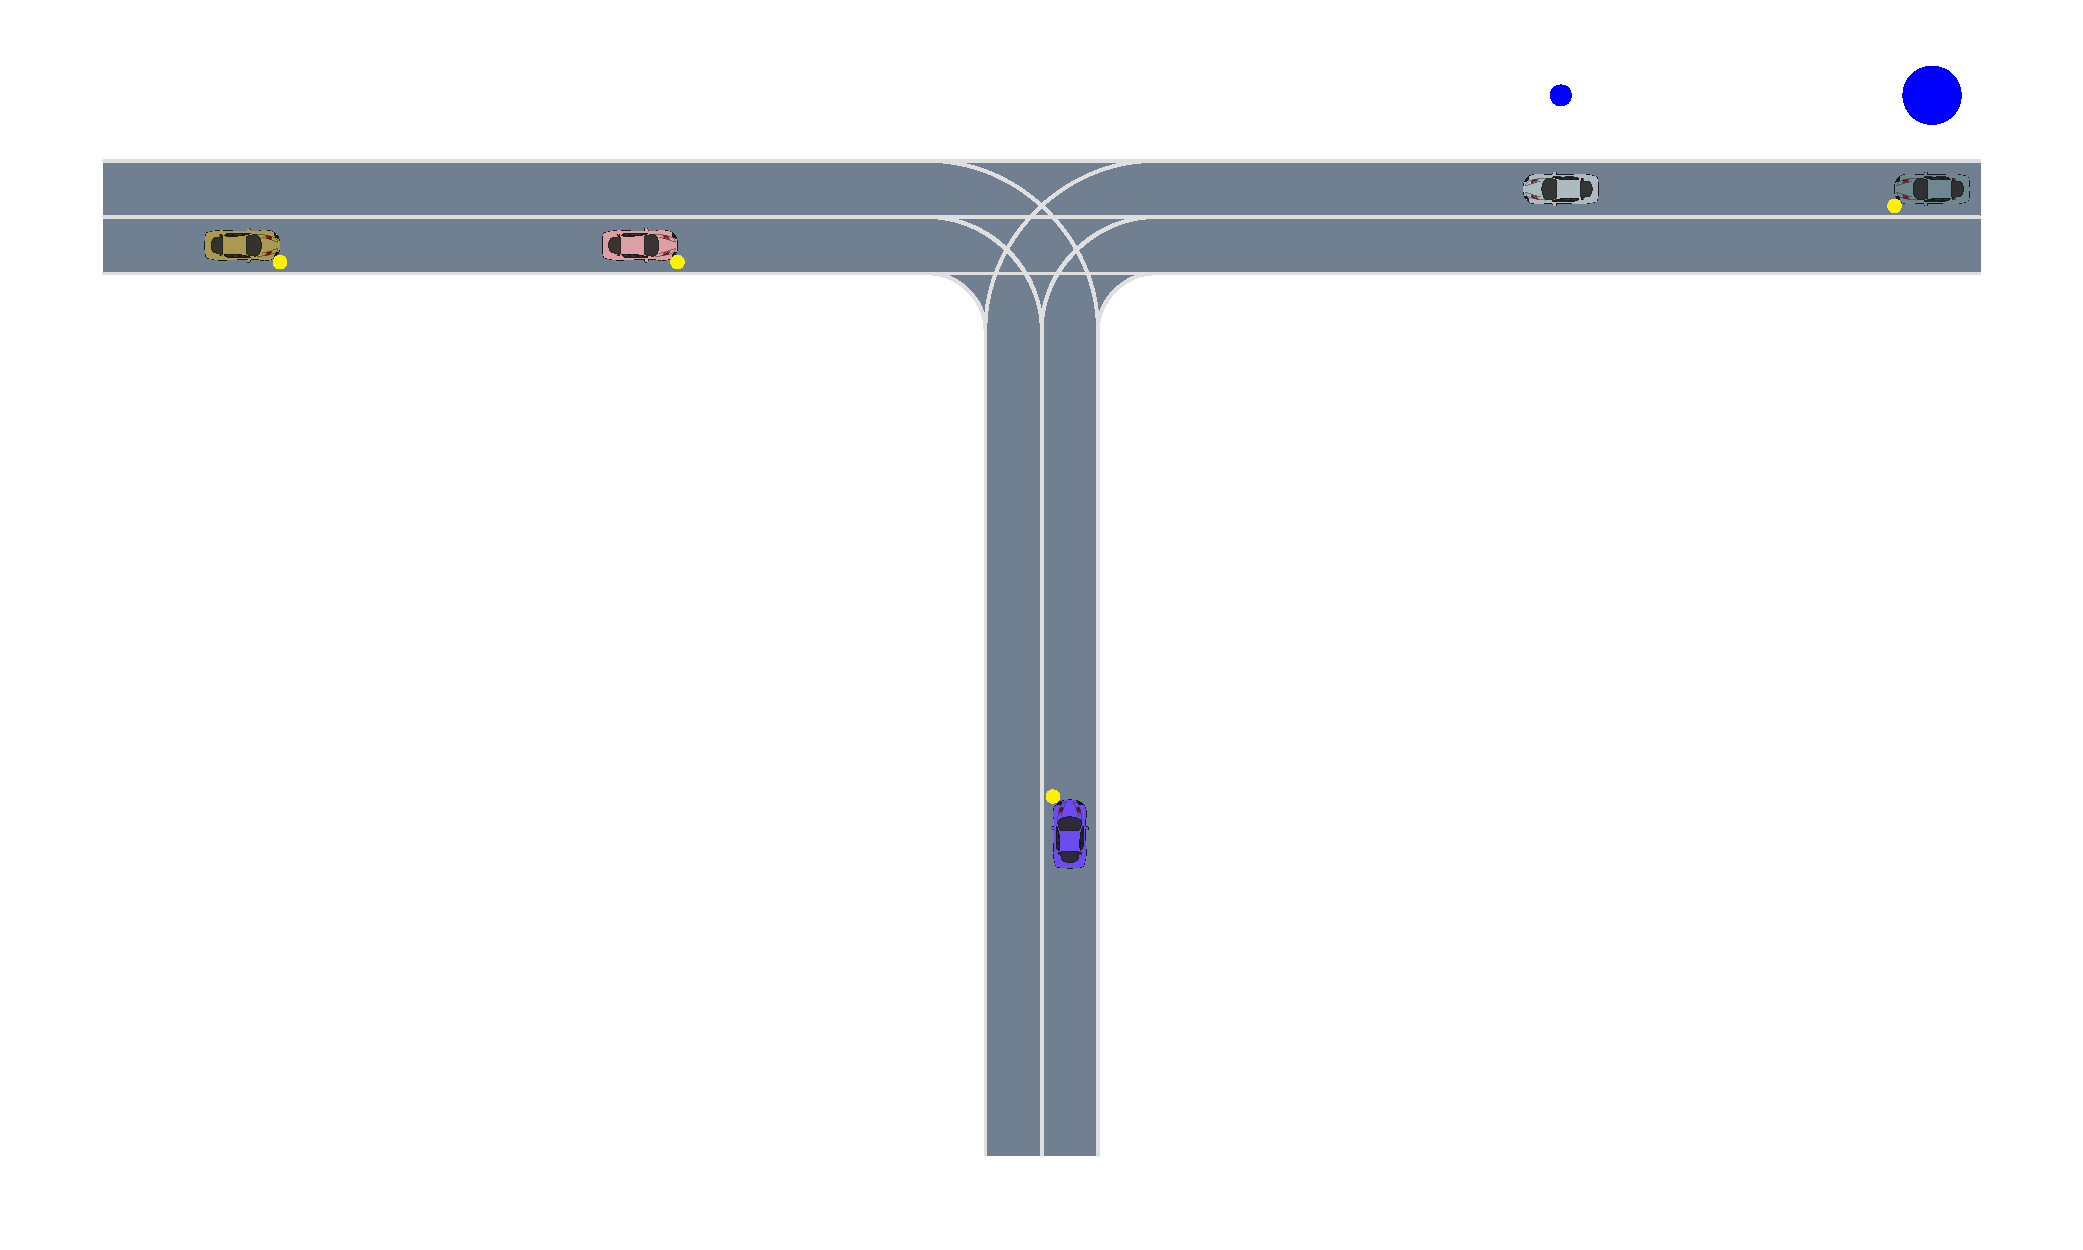
\includegraphics[width=\textwidth, trim={2cm 5cm 1cm 0},clip]{figures/problem_decomposition/f1_1.pdf}
    \end{subfigure}
    \begin{subfigure}[t]{0.7\textwidth}
        \centering
        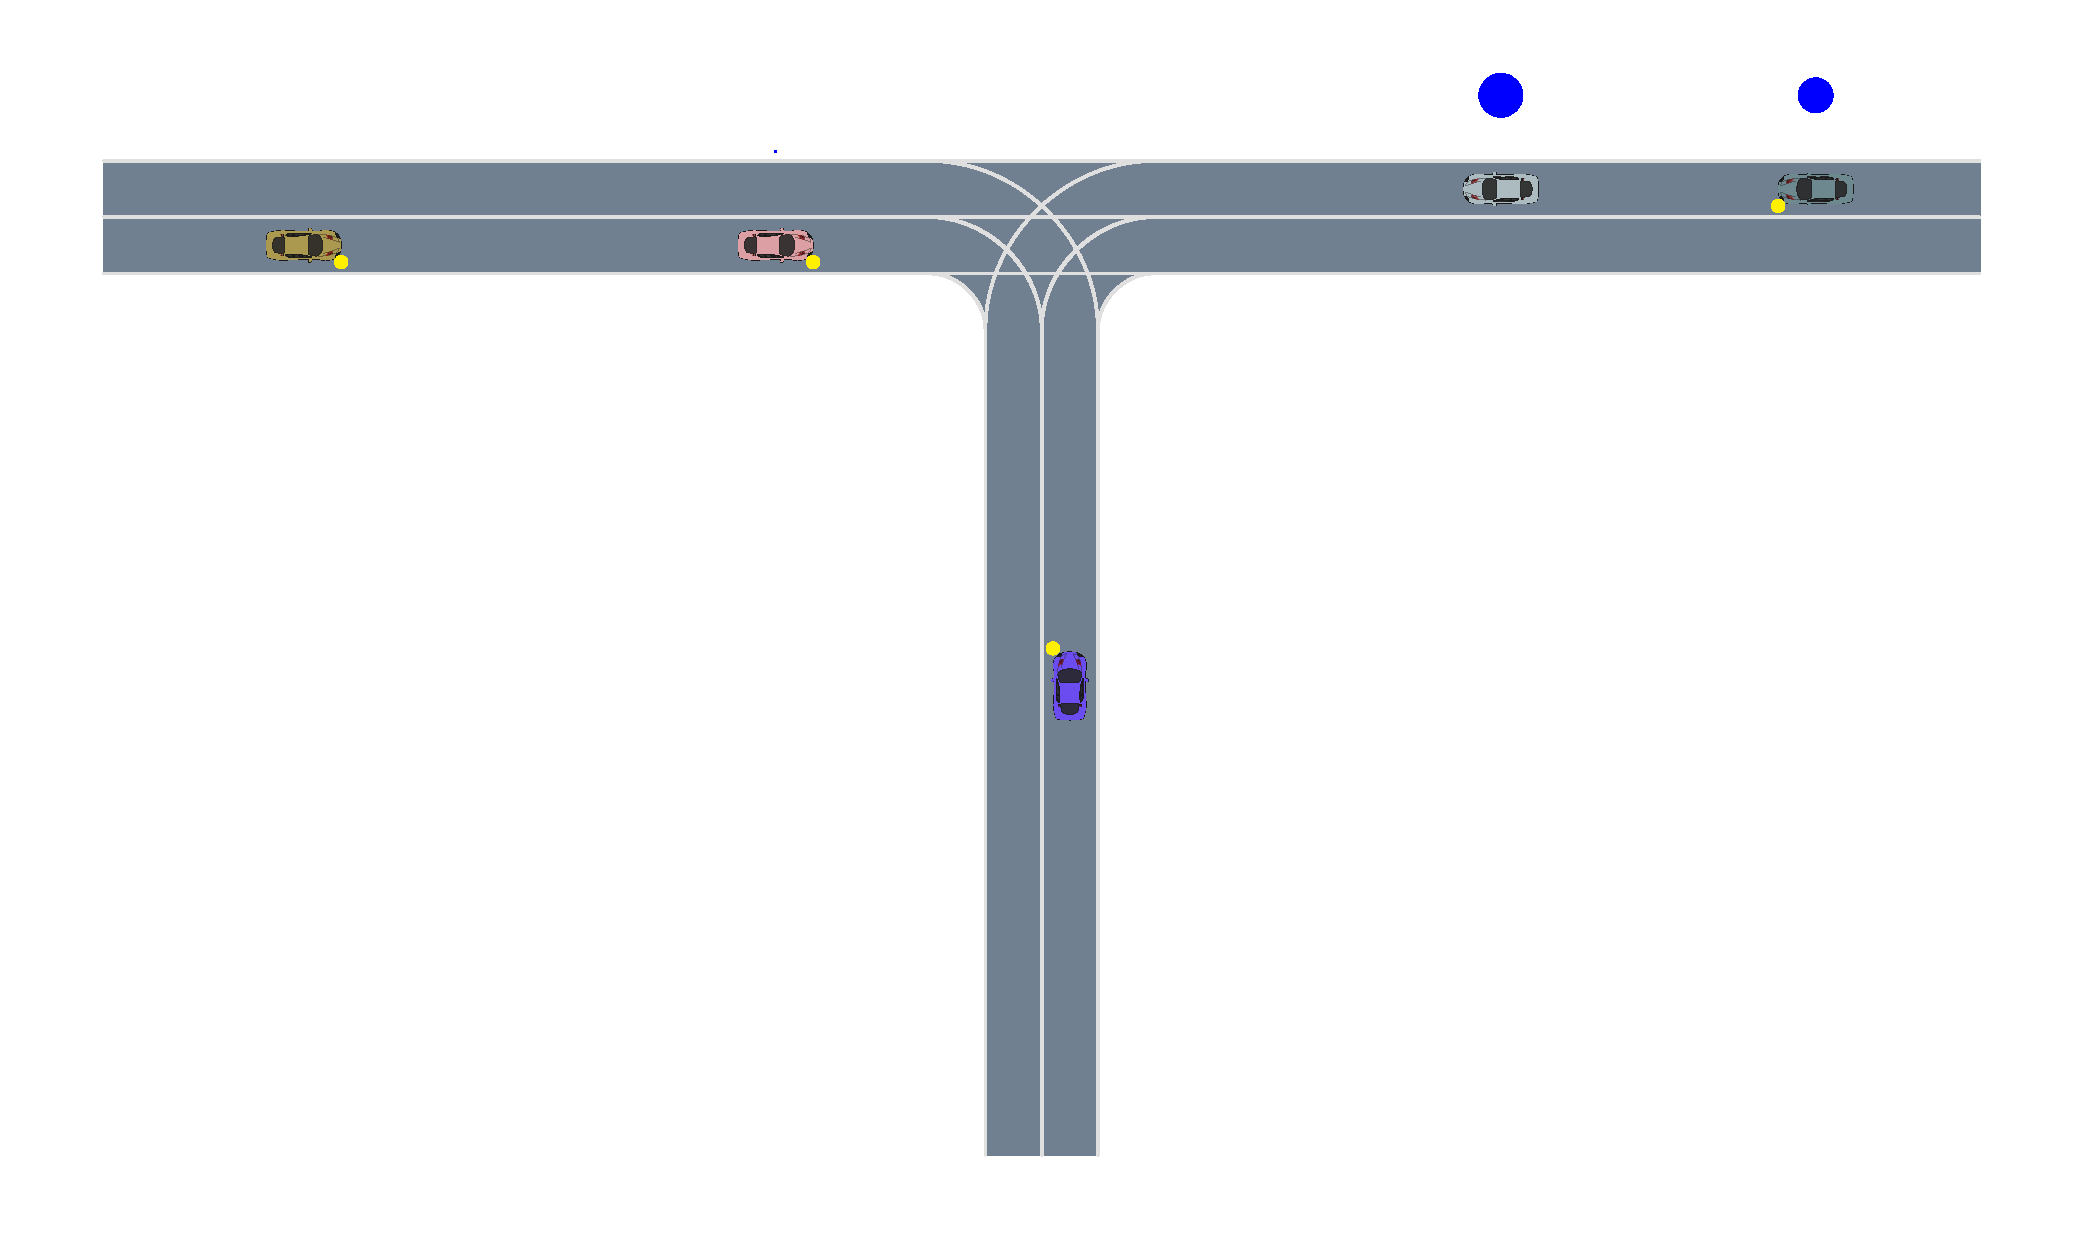
\includegraphics[width=\textwidth, trim={2cm 5cm 1cm 0},clip]{figures/problem_decomposition/f1_4.pdf}
    \end{subfigure}
    \begin{subfigure}[t]{0.7\textwidth}
    \centering
    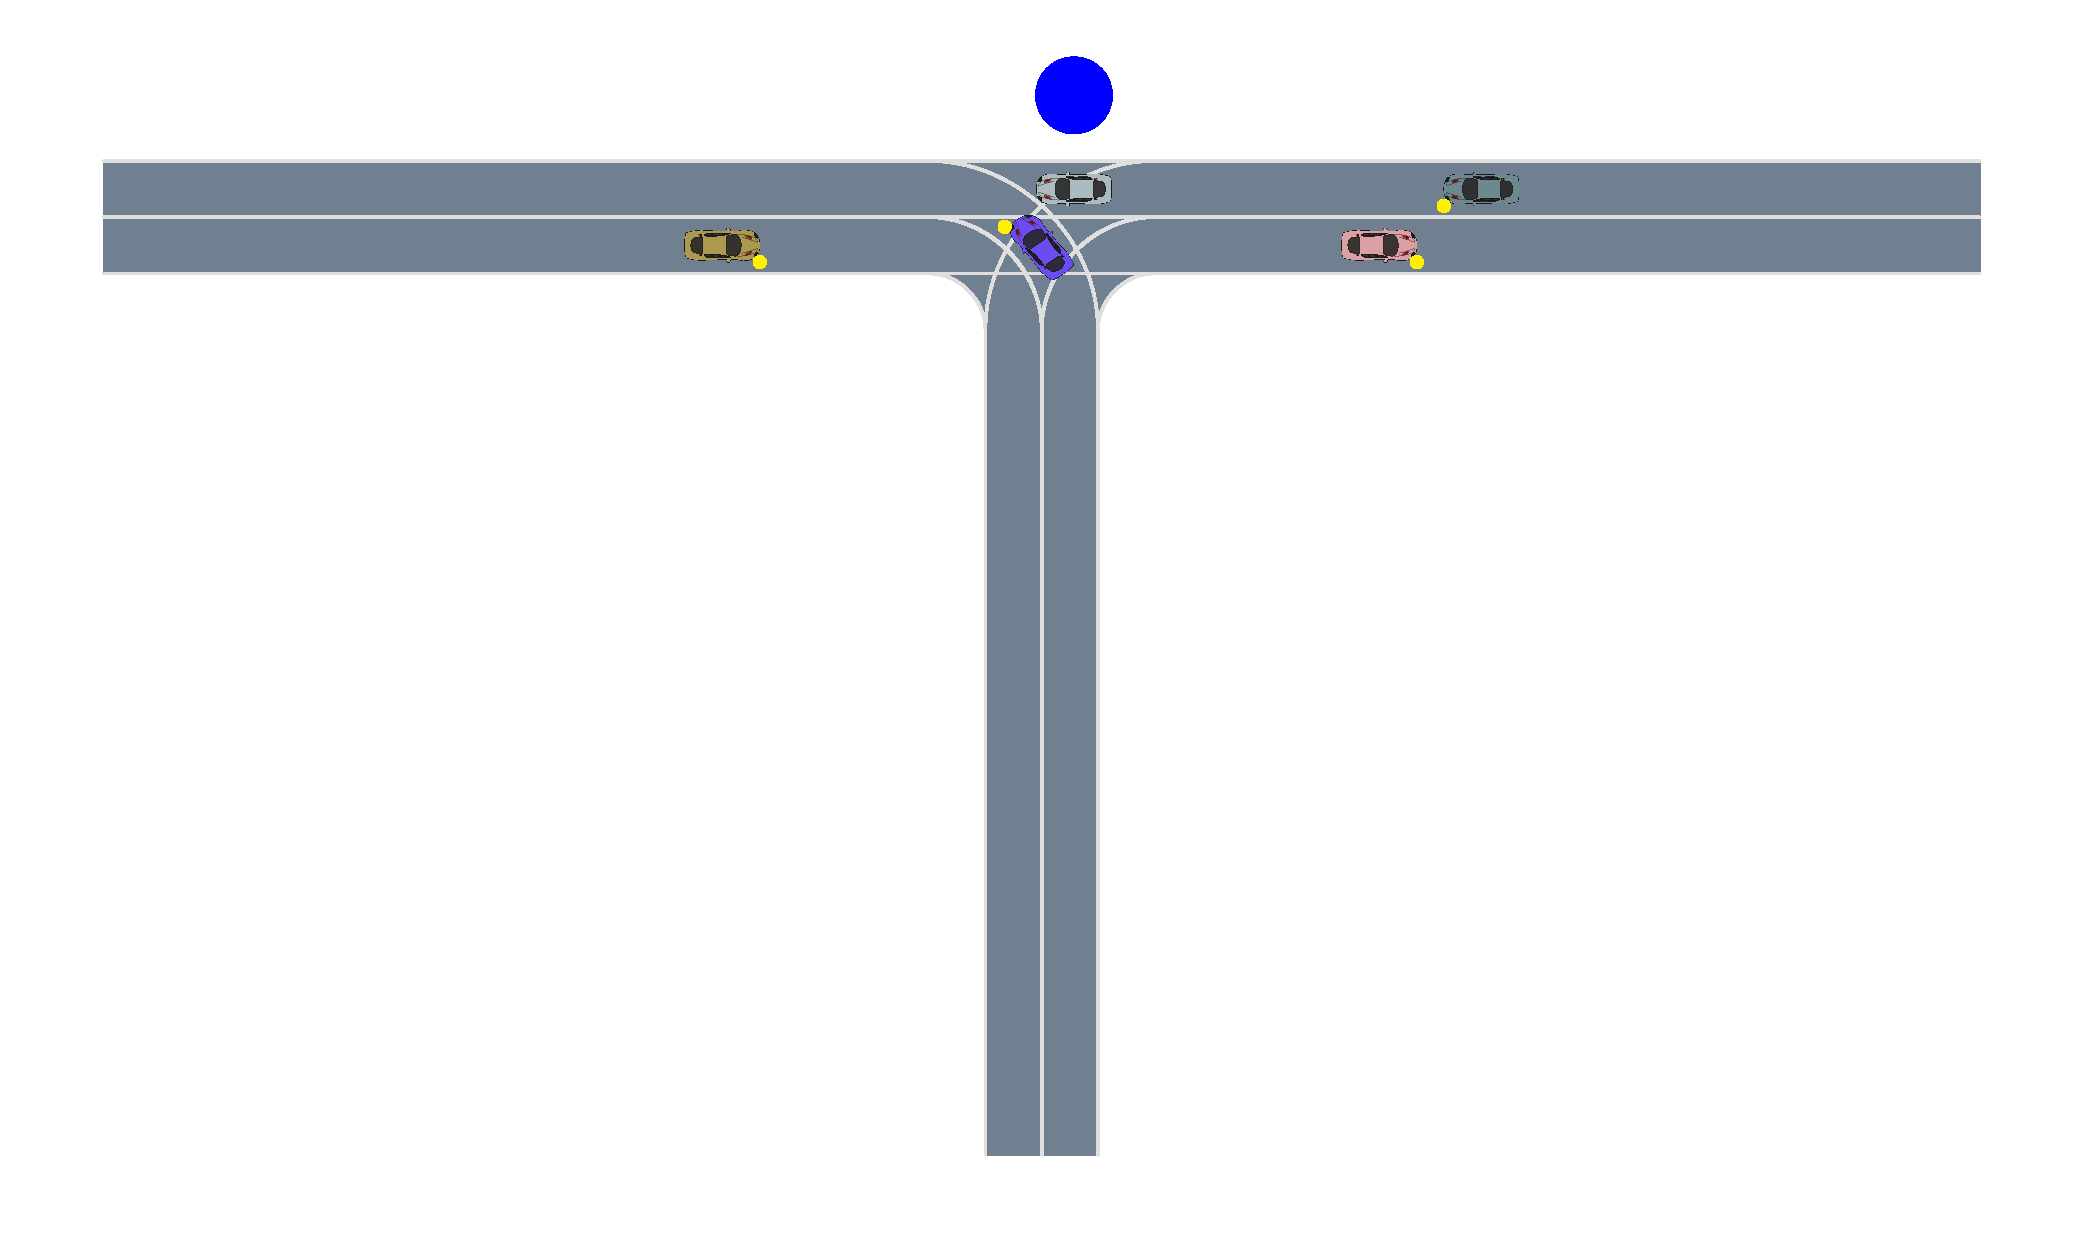
\includegraphics[width=\textwidth, trim={2cm 5cm 1cm 0},clip]{figures/problem_decomposition/f1_18.pdf}
\end{subfigure}
    \caption{Collision in 5-car scenario at timesteps $t=[1,4,18]$.}
    \label{fig:five_car_collision1}
    \vspace{-0.2in}
\end{figure}


\begin{figure}
    \centering
   \begin{subfigure}[t]{0.7\textwidth}
        \centering
        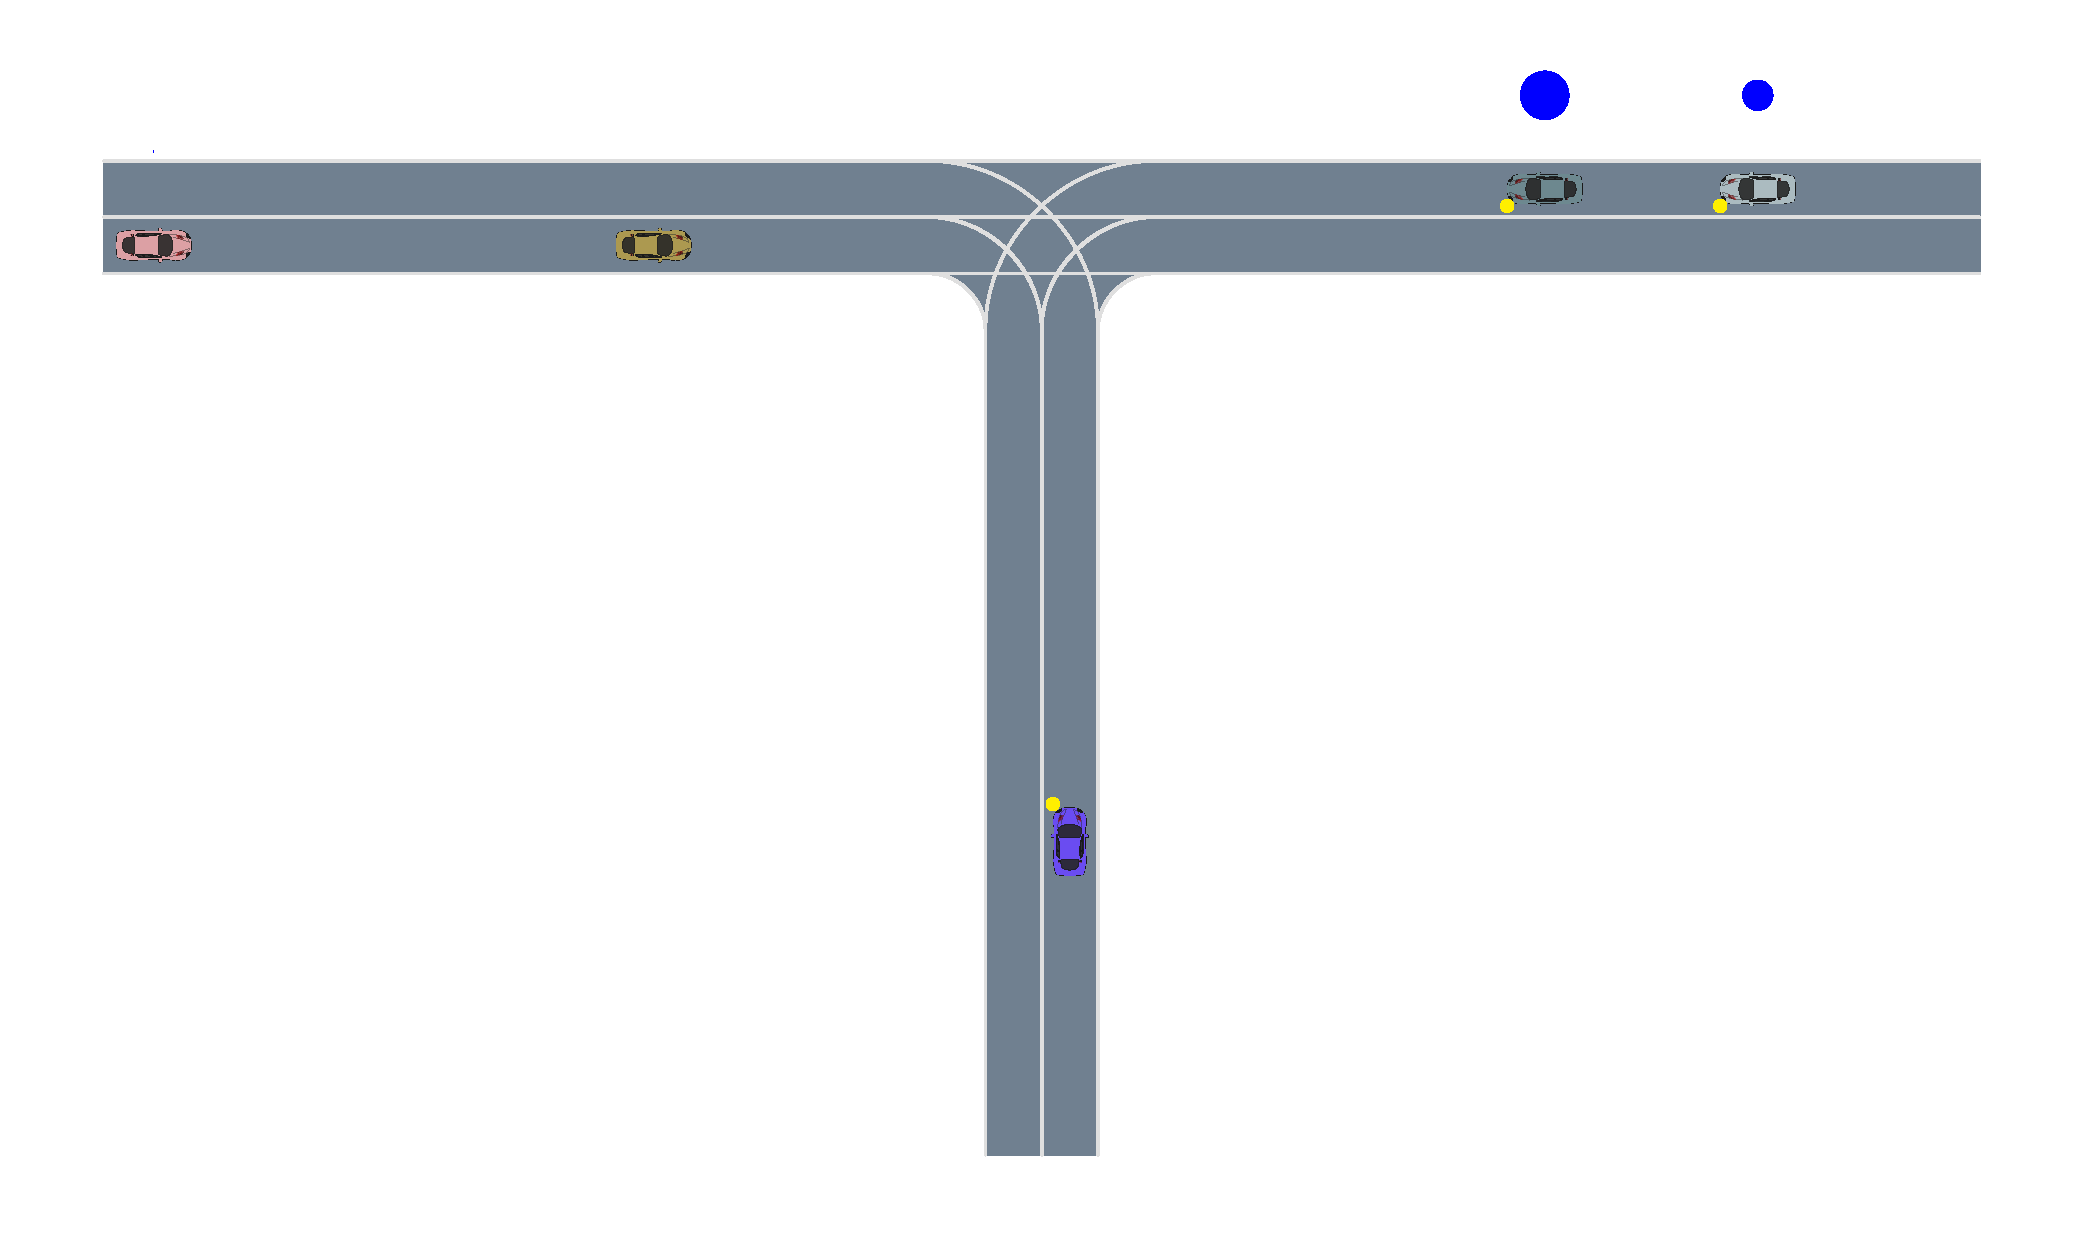
\includegraphics[width=\textwidth, trim={2cm 5cm 1cm 0},clip]{figures/problem_decomposition/f2_1.pdf}
    \end{subfigure}
    \begin{subfigure}[t]{0.7\textwidth}
        \centering
        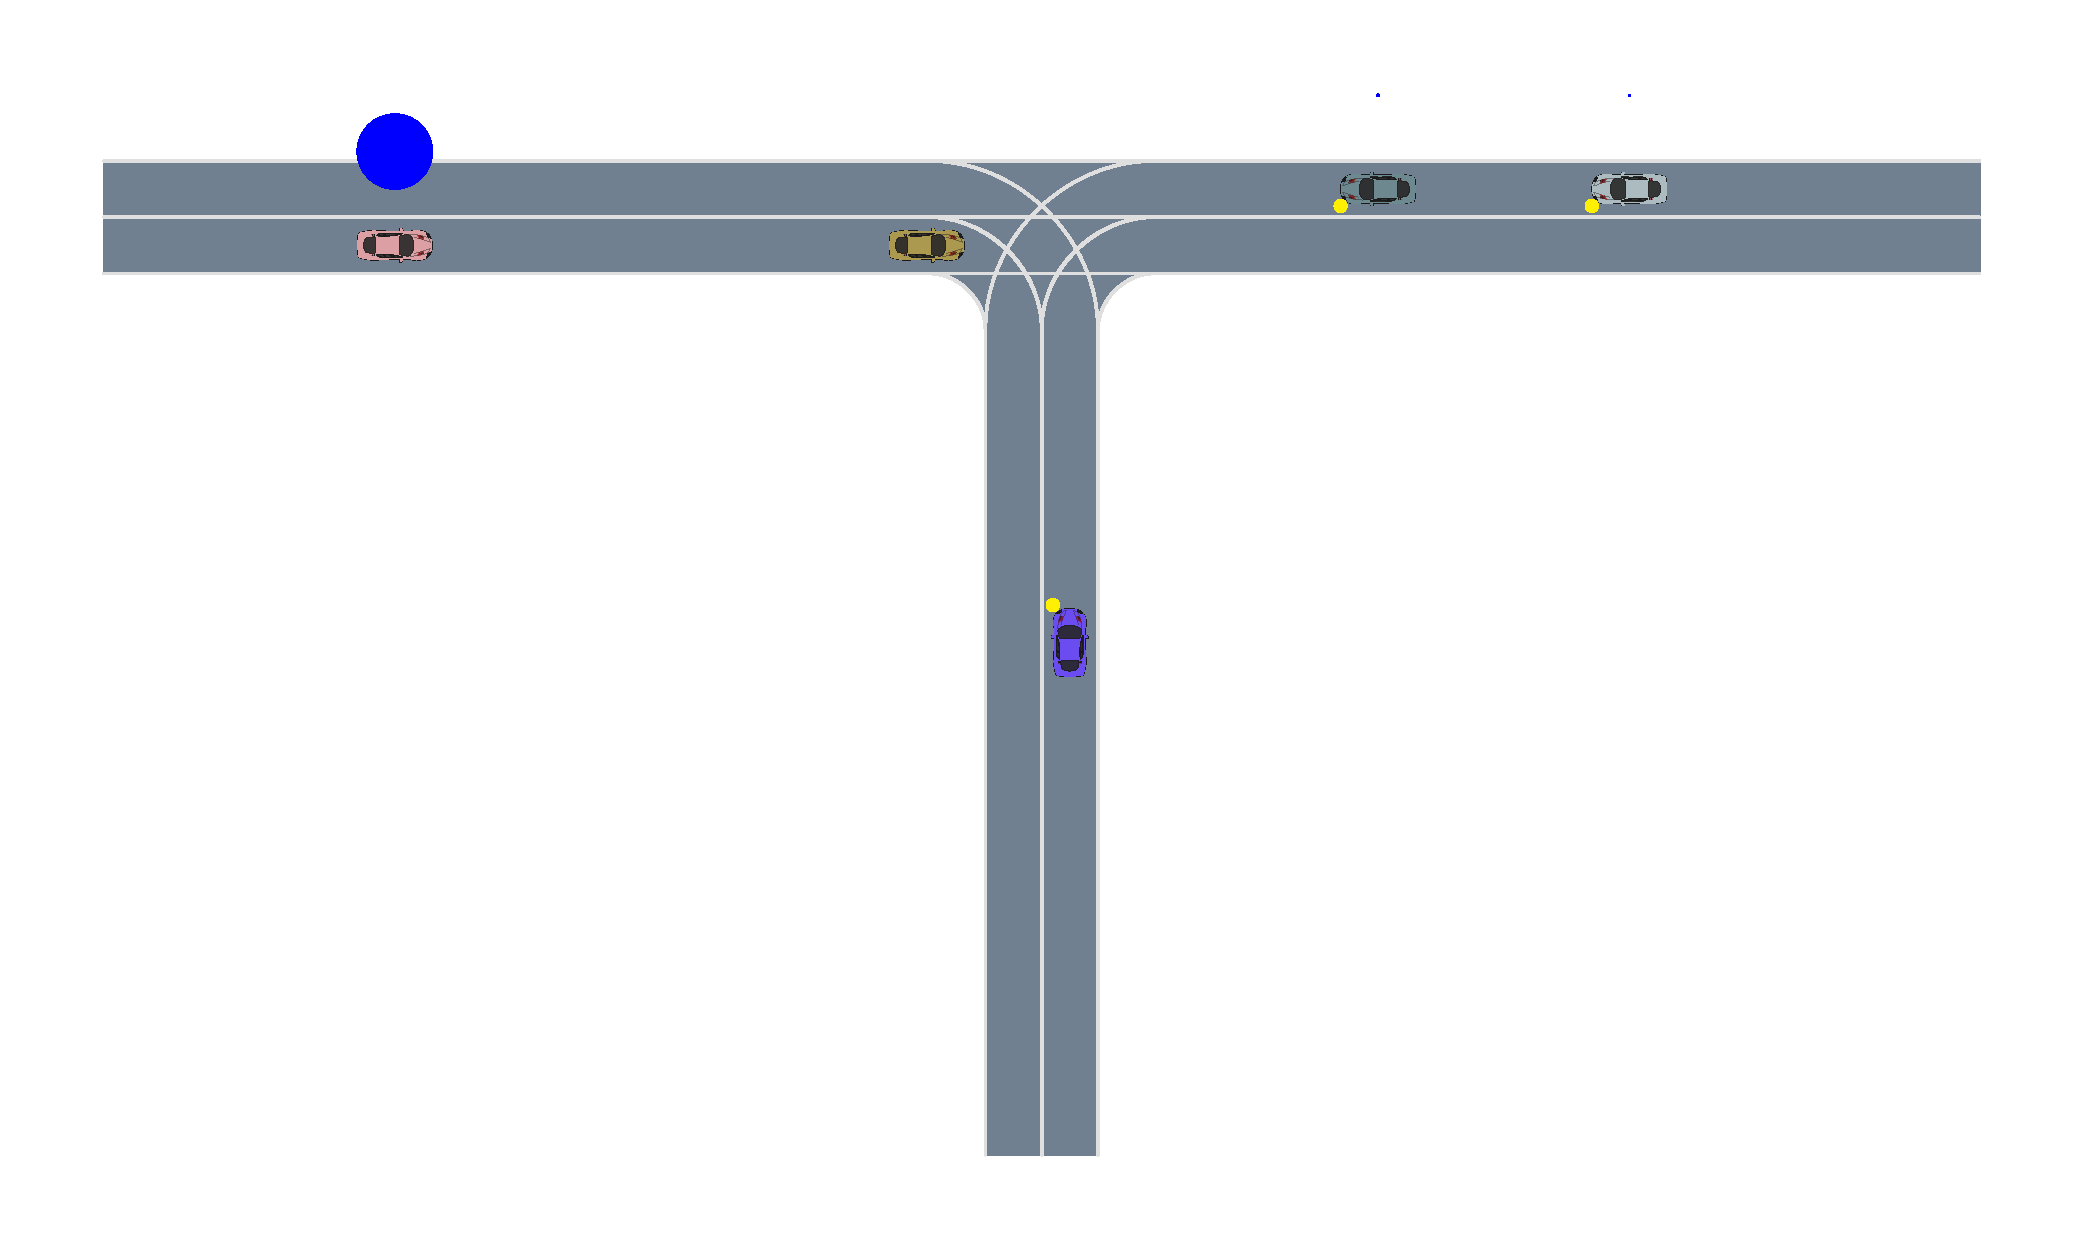
\includegraphics[width=\textwidth, trim={2cm 5cm 1cm 0},clip]{figures/problem_decomposition/f2_8.pdf}
    \end{subfigure}
    \begin{subfigure}[t]{0.7\textwidth}
    \centering
    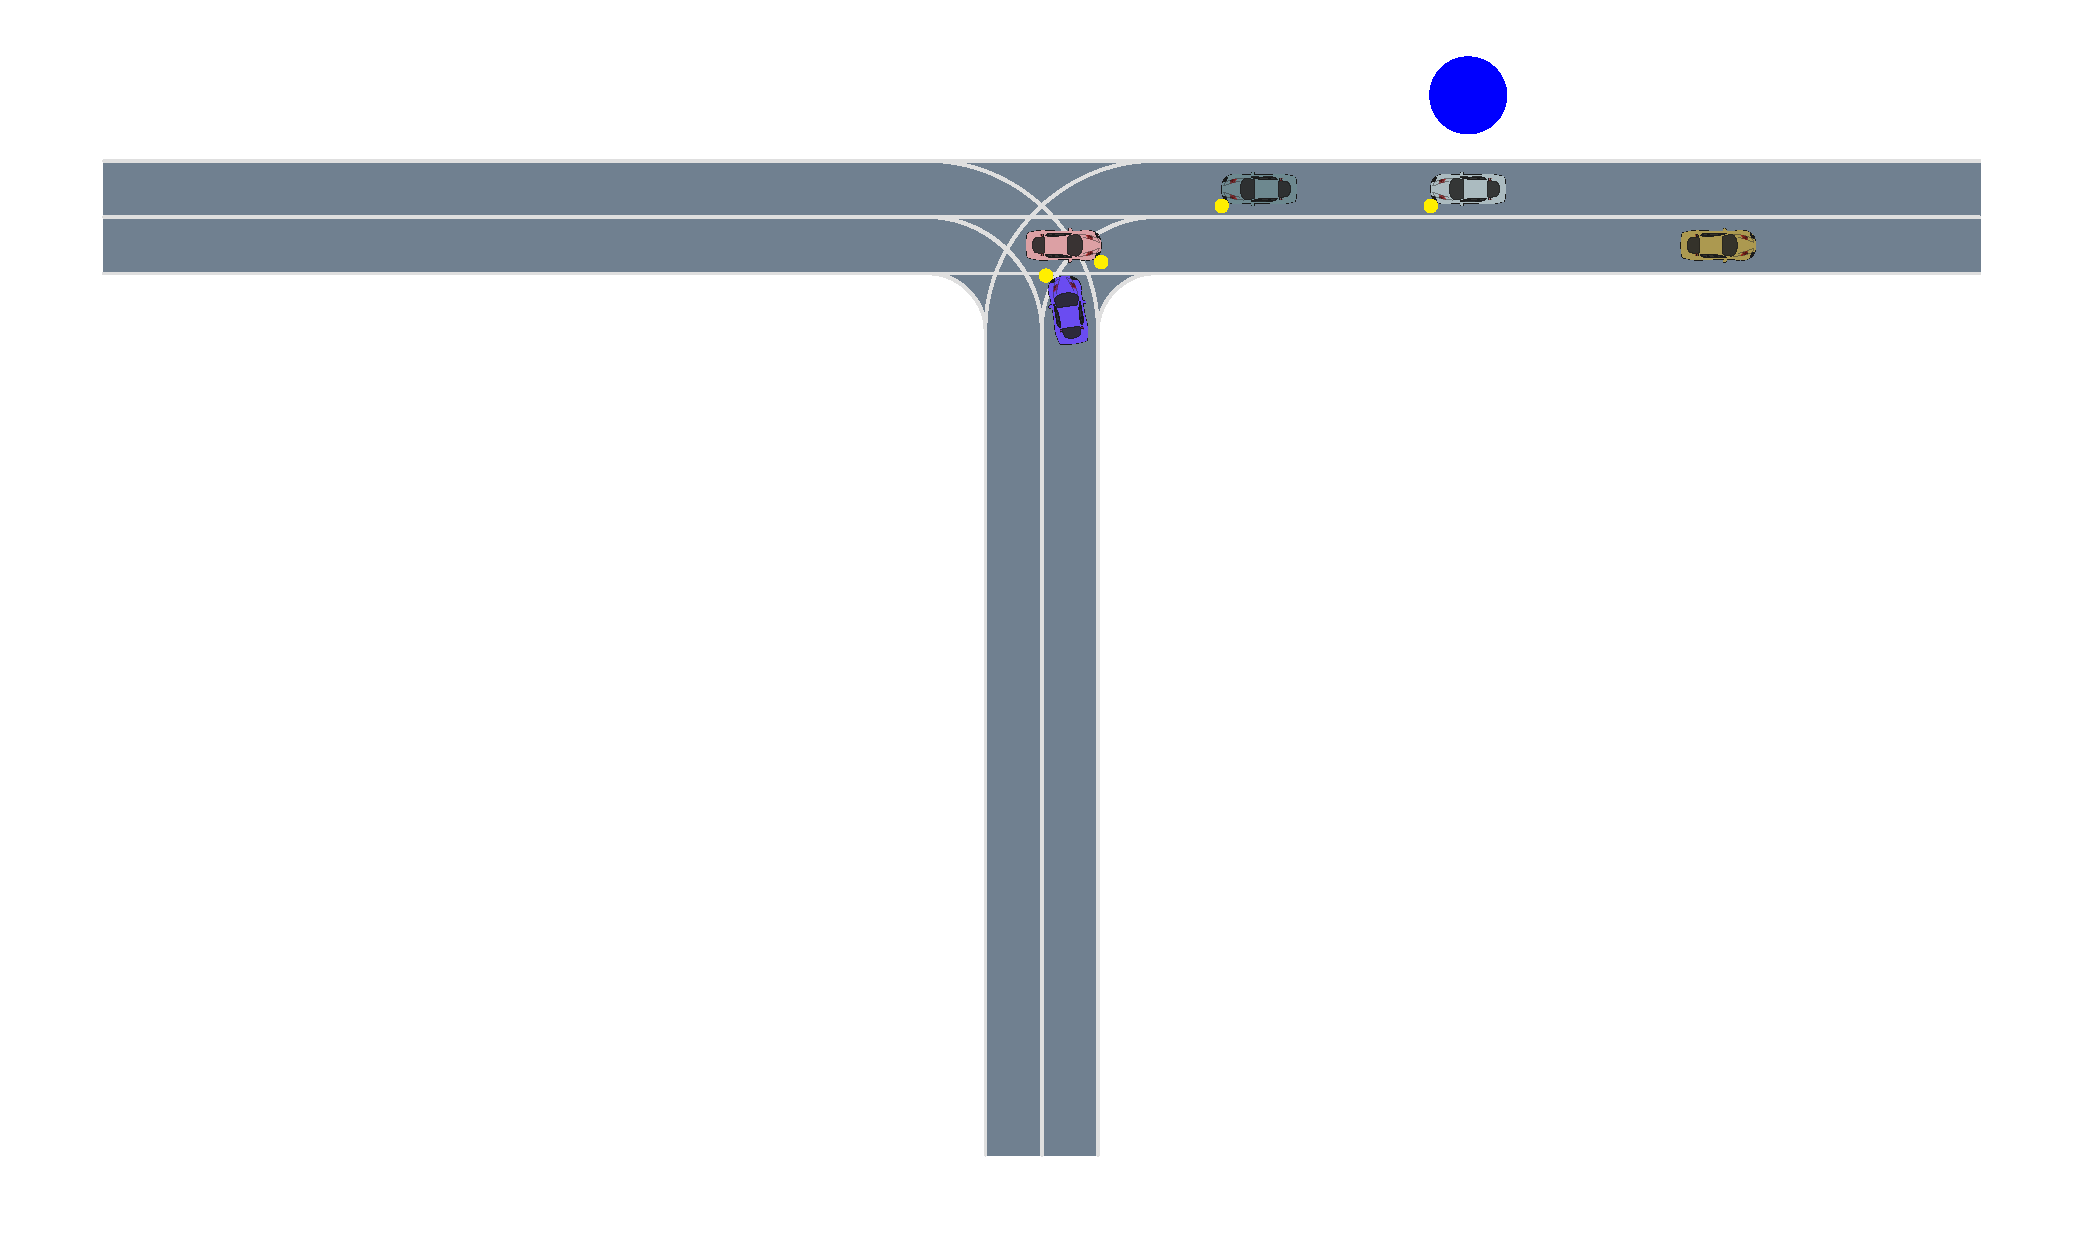
\includegraphics[width=\textwidth, trim={2cm 5cm 1cm 0},clip]{figures/problem_decomposition/f2_27.pdf}
\end{subfigure}
    \caption{Collision in 5-car scenario at timesteps $t=[1,8,27]$.}
    \label{fig:five_car_collision2}
    \vspace{-0.2in}
\end{figure}


\section{Discussion}

% Summary
Multi-agent safety validation problems pose a challenge for safety validation algorithms due to the large state and actions paces. In this chapter we made a step toward the scalability of safety validation algorithms to multi-agent settings by applying problem decomposition. We discussed a technique for decomposing a multi-agent system into tractable subproblems and then combining the solutions using the attend, adapt and transfer architecture. 

Using the ground truth of simple multi-agent gridworld problem, we showed that estimates of the probability of failure of the \num{3}-agent system were improved by referencing the probability of failure of the \num{2}-agent system. We then applied the decomposition approach to the T-intersection scenario with \num{4} adversaries. By decomposing the problem into two unique subproblems and recombining their solutions, we were able to approximate the distribution over failures and outperform baseline approaches. 

In addition to the transfer learning literature, our approach to scene decomposition is also similar to the work of \textcite{bouton2019decomposition}. In that work they perform a similar pairwise decomposition to help train a safe driving policy. Each subproblem was solved for the optimal value function and the results were fused with simple aggregated by taking the max or mean. To account for multi-agent interactions, they learned an additive correction factor parameterized by a deep neural network. The A2T approach is more flexible because the combination of subproblem solutions is learned and state dependent. Unlike training an agent to drive, in the safety validation problem the action space scales with the number of agents, which adds an additional challenge to overcome.

In the next chapter we turn away from solving individual safety validation problems and consider the problem of iterative safety validation. We demonstrate that we can gain significant performance and efficiency improvement by storing and reusing safety validation knowledge across systems. 